% Based on format by Jos� Koiller
% Updated by Daniel Foreman-Mackey

%% Use the first of the following lines during production to
%% easily spot "overfull boxes" in the output. Use the second
%% line for the final version.
% \documentclass[12pt,draft,letterpaper]{report}
\documentclass[12pt,letterpaper]{report}

\newcommand{\thesistitle}{Probabilistic methods for cosmology \\
	using uncertainty-dominated data}
\newcommand{\thesisauthor}{Alex I. Malz}
\newcommand{\thesisadvisor}{Professor David W. Hogg}
\newcommand{\graddate}{May 2019}

%% The following makes chapters and sections, but not subsections,
%% appear in the TOC (table of contents). Increase to 2 or 3 to
%% make subsections or subsubsections appear, respectively. It seems
%% to be usual to use the "1" setting, however.
\setcounter{tocdepth}{1}

%% Sectional units up to subsubsections are numbered. To number
%% subsections, but not subsubsections, decrease this counter to 2.
\setcounter{secnumdepth}{3}

%% Page layout (customized to letter paper and NYU requirements):
\setlength{\oddsidemargin}{0in}
\setlength{\textwidth}{6.5in}
\setlength{\topmargin}{0in}
\setlength{\headheight}{0in}
\setlength{\headsep}{0in}
\setlength{\textheight}{8.3in}
% \setlength{\footskip}{.5in}
\setlength{\skip\footins}{.3in}

\usepackage{setspace}
% \singlespacing{}
\doublespacing{}

%% This inputs your auxiliary file with \usepackage's and \newcommand's:
%% It is assumed that that file is called "definitions.tex".
\RequirePackage[displaymath, mathlines]{lineno}

\usepackage[tbtags]{amsmath}
\usepackage{amssymb}
\usepackage{amsfonts}
\usepackage{amsthm}

\usepackage{color, hyperref}
\definecolor{linkcolor}{rgb}{0,0,0.2}
\hypersetup{colorlinks=true,linkcolor=linkcolor,citecolor=linkcolor,
            filecolor=linkcolor,urlcolor=linkcolor}
\hypersetup{pageanchor=false}

\usepackage{indentfirst}
\usepackage{booktabs}
\usepackage{url}
\usepackage{multirow}
\usepackage{xspace}
\usepackage{enumitem}
\usepackage[final]{graphicx}
\usepackage{wasysym}

\usepackage{footmisc}
\usepackage{soul}

\usepackage{tikz}
\usetikzlibrary{shapes.geometric, arrows}
\usetikzlibrary{fit}

\tikzstyle{hyper} = [circle, text centered, draw=black]
\tikzstyle{param} = [circle, text centered, draw=black]
\tikzstyle{data} = [circle, text centered, draw=black, line width=2pt]
\tikzstyle{arrow} = [thick,->,>=stealth]

% Custom AAS macros:
\usepackage{aas_macros}
\usepackage{lsstdesc_macros}

% Bibliography:
\usepackage{natbib}
\bibliographystyle{apj}

% Algorithms:
\usepackage{algorithmic, algorithm}

% Thesis-specific:
\newcommand{\thesistitle}{Probabilistic analysis methods for cosmology \\
	using uncertainty-dominated photometric data}
\newcommand{\thesisauthor}{Alex I. Malz}
\newcommand{\thesisadvisor}{Professor David W. Hogg}
\newcommand{\graddate}{May 2019}

% Commands:

% General formatting:
\newcommand{\paper}{Chapter}
%\newcommand{\textul}[1]{{\underline{#1}}}
\newcommand{\mathul}[1]{\underline{#1}}
\newcommand{\enquote}[1]{{``{#1}''}}

% Foreign text:
\newcommand{\foreign}[1]{\emph{#1}}
%\newcommand{\etal}{\foreign{et\,al.}}
%\newcommand{\etc}{\foreign{etc.}}

% Project references:
\newcommand{\project}[1]{{\textsc{#1}}}
\newcommand{\lsst}{\project{LSST}}
\newcommand{\desc}{\project{LSST-DESC}}
\newcommand{\coin}{\project{COIN}}
\newcommand{\sdss}{\project{SDSS}}
\newcommand{\des}{\project{DES}}

% Code references:
\newcommand{\repo}[1]{{\texttt{#1}}}
\newcommand{\qp}{\repo{qp}}
\newcommand{\chippr}{\repo{chippr}}

% Tools:
\newcommand{\github}{\href{https://github.com}{GitHub}}
\newcommand{\python}{\textit{Python}}

% LaTeX object referencing:
\newcommand{\chapid}{no chapter}
\renewcommand{\figref}[1]{\ref{\chapid:fig:#1}}
\newcommand{\Fig}[1]{Figure~\figref{#1}}
\newcommand{\fig}[1]{\Fig{#1}}
\newcommand{\figlabel}[1]{\label{\chapid:fig:#1}}

\newcommand{\Tab}[1]{Table~\ref{\chapid:tab:#1}}
\newcommand{\tab}[1]{\Tab{#1}}
\newcommand{\tablabel}[1]{\label{\chapid:tab:#1}}

\renewcommand{\eqref}[1]{\ref{\chapid:eq:#1}}
\newcommand{\Eq}[1]{Equation~(\eqref{#1})}
\newcommand{\eq}[1]{\Eq{#1}}
\newcommand{\eqalt}[1]{Equation~\eqref{#1}}
\newcommand{\eqlabel}[1]{\label{\chapid:eq:#1}}

\newcommand{\sectionname}{Section}
\newcommand{\sectref}[1]{\ref{\chapid:sect:#1}}
\newcommand{\Sect}[1]{\sectionname~\sectref{#1}}
\newcommand{\sect}[1]{\Sect{#1}}
\newcommand{\sectalt}[1]{\sectref{#1}}
\newcommand{\App}[1]{Appendix~\sectref{#1}}
\newcommand{\app}[1]{\App{#1}}
\newcommand{\sectlabel}[1]{\label{\chapid:sect:#1}}

\newcommand{\Algo}[1]{Algorithm~\ref{\chapid:algo:#1}}
\newcommand{\algo}[1]{\Algo{#1}}
\newcommand{\algolabel}[1]{\label{\chapid:algo:#1}}

\newcommand{\chapname}{Chapter}
\newcommand{\Chap}[1]{\chapname~\ref{chap:#1}}
\newcommand{\chap}[1]{\Chap{#1}}
\newcommand{\chapalt}[1]{\ref{chap:#1}}
\newcommand{\chaplabel}[1]{\label{chap:#1}}

\newcommand{\todo}[3]{{\color{#2}\emph{#1}: #3}}
\newcommand{\aim}[1]{\todo{AIM}{red}{#1}}

\newtheorem{theorem}{Theorem}[section]
\newtheorem{proposition}[theorem]{Proposition}
\newtheorem{lemma}[theorem]{Lemma}
\newtheorem{corollary}[theorem]{Corollary}
\newtheorem{conjecture}[theorem]{Conjecture}

\theoremstyle{definition}
\newtheorem{definition}[theorem]{Definition}
\newtheorem{remark}[theorem]{Remark}
\newtheorem{example}[theorem]{Example}

% Math:
%\newcommand{\dd}{\ensuremath{\,\mathrm{d}}}
\newcommand{\bvec}[1]{{\ensuremath{\boldsymbol{#1}}}}% could change to \vec
%\newcommand{\paramvector}[1]{\bvec{#1}}
%\newcommand{\unit}[1]{\mathrm{#1}}
\newcommand{\data}{\ensuremath{\vec{d}}}% could change to bold

% Probabilities:
\newcommand{\perm}[2]{\ensuremath{_{#1}\mathrm{P}_{#2}}}
\newcommand{\comb}[2]{\ensuremath{_{#1}\mathrm{C}_{#2}}}
\newcommand{\like}{\mathscr{L}}
\newcommand{\pr}[1]{\ensuremath{p(#1)}}% could change to Prob or Pr 
\newcommand{\expect}[1]{\left<#1\right>}
\newcommand{\normal}[2]{\mathcal{N} (#1, #2)}
\newcommand{\gvn}{\mid}% could use | or \vert
\newcommand{\integral}[2]{\ensuremath{\int\ #1\ \mathrm{d} #2}}

% misc science
\newcommand{\sz}{spec-$z$}
\newcommand{\Sz}{Spec-$z$}
\newcommand{\pz}{photo-$z$}
\newcommand{\Pz}{Photo-$z$}
\newcommand{\pzpdf}{\pz\ PDF}% could change to posterior
\newcommand{\Pzpdf}{\Pz\ PDF}% could change to posterior
\newcommand{\zpdf}{redshift posterior}% could change to implicit posterior
\newcommand{\pzip}{\pz\ implicit posterior}
\newcommand{\nz}{$n(z)$}
\newcommand{\Nz}{$N(z)$}
\newcommand{\stack}{$\hat{N}(z)$}

\sloppy\sloppypar


\begin{document}

%% Produces a test "layout" page, for "debugging" purposes only.
%% Comment out for final version.
% \layout  % requires package layout (see above, on this same file)

%%%%%% Title page %%%%%%%%%%%
%% Sets page numbering to "roman style" i, ii, iii, iv, etc:
\pagenumbering{roman}
%
%% No numbering in the title page:
\thispagestyle{empty}
%
\begin{center}


    \vspace*{0.5in}
    {\large\textbf{\thesistitle}}
    \vspace{.4in}

    by
    \vspace{.4in}

    \thesisauthor{}
    \vspace{.8in}
    % \vfill

    \begin{doublespace}
        A dissertation submitted in partial fulfillment \\
        of the requirements for the degree of \\
        Doctor of Philosophy \\
        Department of Physics \\
        New York University \\
        \graddate{}
    \end{doublespace}
\end{center}
\vfill

\noindent\makebox[\textwidth]{\hfill\makebox[2.5in]{\hrulefill}}\\
\makebox[\textwidth]{\hfill\makebox[2.5in]{\hfill\thesisadvisor\hfill}}
\newpage

% %%%%%%%%%%%%%% Copyright %%%%%%%%%%%%%%%%%
\vspace*{\fill}
\begin{center}
    Copyright \textcopyright\ 2019 Alex I. Malz \\
    This work is licensed under a Creative Commons Attribution 4.0
    International License.
    \addcontentsline{toc}{section}{Copyright}
\end{center}
\vfill
\newpage

%%%%%%%%%%%%% Blank page %%%%%%%%%%%%%%%%%%
\thispagestyle{empty}
\vspace*{0in}
\newpage

%%%%%%%%%%%%%% Acknowledgements %%%%%%%%%%%%
%% Comment out the following lines if you do not want to acknowledge
%% anyone's help...
\section*{Acknowledgements}\addcontentsline{toc}{section}{Acknowledgements}
%% Write your acknowledgements in this file. If you do not want to acknowledge anyone,
%% you can delete this file and comment out the corresponding part in the "thesis.tex"
%% file.
%
I would like to acknowledge the effort put into this thesis by
myself. This work could not have been done without me.

\newpage

%%%%%%%%%%%%%% Quotation Page %%%%%%%%%%%%
\vspace*{0.2\textheight}
% \noindent\enquote{\itshape }\bigbreak
% \hfill 
\noindent\enquote{\itshape Somewhere, something incredible is waiting to be known.}\\
\hfill Carl Sagan\\

\bigbreak

\noindent\enquote{\itshape If we knew what it was we were doing, it would not be called research, would it?}\\
\hfill Albert Einstein\\
\newpage

%%%% Abstract %%%%%%%%%%%%%%%%%%
\section*{Abstract}\addcontentsline{toc}{section}{Abstract}
The study of exoplanets has been revolutionized in recent years thanks, in
large part, to new data collected by NASA's \emph{Kepler} Mission.
The Mission has enabled the discovery of thousands of planets orbiting stars
throughout the Galaxy.
These discoveries span orders of magnitude in physical parameter space but
many of the most physically interesting questions remain open.
The deepest of these questions is: how common are planetary systems like our
own Solar System?
In this dissertation, I approach this question from several different angles
and make inferences about the frequency and distribution of planets based on
the large, publicly-available datasets from the \emph{Kepler} Mission.

I develop two powerful and practical methods for mining for planetary transit
signals in the hundreds of thousands of stellar light curves measured by
\emph{Kepler}.
The first method is designed to find planets using the data from the
\emph{K2} phase of the Mission where systematics introduced by the instrument
dominate the measurements.
Applying this method to the first publicly available dataset from \emph{K2},
Campaign 1, I published more than thirty new exoplanet candidates.
The second transit search technique is designed to find transits of planets
with orbital periods longer than the four year baseline of the \emph{Kepler}
Mission.
These are interesting planets because they are expected to have the largest
dynamical influence on the formation and evolution of their planetary systems
but, to date, no systematic search for these signals has been published.
I demonstrate that this method is robust and tractable and make predictions
for the planet yields in the \emph{Kepler} dataset.

I derive a general framework for making justified probabilistic inferences
about the population of planets based on noisy and incomplete catalogs of
exoplanet measurements.
Applying this to a previously published catalog of exoplanets orbiting stars
like our Sun, I measure the joint period--radius distribution of these
planets taking into account survey selection effects and the large
measurement uncertainties.
Despite the fact that this catalog includes no true Earth analogs, I use the
detected systems and weak smoothness assumptions about the underlying
distribution to make a probabilistic estimate of the frequency of Earth-like
planets.

\newpage

%%%% Table of Contents %%%%%%%%%%%%
\tableofcontents

%%%%% List of Figures %%%%%%%%%%%%%
%% Comment out the following two lines if your thesis does not
%% contain any figures. The list of figures contains only
%% those figures included withing the "figure" environment.
\newpage\addcontentsline{toc}{section}{List of Figures}
\listoffigures

%%%%% List of Tables %%%%%%%%%%%%%
%% Comment out the following two lines if your thesis does not
%% contain any tables. The list of tables contains only
%% those tables included withing the "table" environment.
\newpage\addcontentsline{toc}{section}{List of Tables}
\listoftables
\newpage

%%%%% Body of thesis starts %%%%%%%%%%%%
\pagenumbering{arabic}

%% Introduction. If your thesis has no introduction, or chapter 1 is
%% meant to be the introduction, then comment out the lines below.
\chapter*{Introduction}\addcontentsline{toc}{chapter}{Introduction}

%[Why do we need redshifts? cosmology problems and galaxy evolution, use as distance proxy via Hubble law]

Photometric redshift (\pz) estimation has been a staple of studies of galaxy evolution, large-scale structure, and cosmology since its conception decades ago \citep{Baum1962}.  
An extremely coarse spectrum in the form of photometry in a handful of broadband filters can be an effective substitute for the time- and photon-intensive process of obtaining a spectroscopic redshift (\sz), a procedure that may only be applied to relatively bright galaxies.  
Once the photometric colors are calibrated against either a library of spectral energy distribution (SED) templates or a data set of spectra for galaxies with known redshifts, a correspondence between photometric colors and redshifts may be constructed, forming a trustworthy basis for \pz\ estimation or testing.

Many more \pz s may be obtained in the time it would take to observe a smaller number of \sz s, and \pz s may be measured for galaxies too dim for accurate \sz\ confirmation, permitting the compilation of large surveys of galaxy redshifts spanning a broad range of redshifts and luminosities.  
\Pz s have thus enabled the era of precision cosmology, heralded by weak gravitational lensing tomography and baryon acoustic oscillation peak measurements.  
Calculations of correlation functions of cosmic shears and galaxy positions require large numbers of high-confidence redshifts of surveyed galaxies.  

However, \pz s are susceptible to inaccuracy and imprecision via a number of effects, particularly their inherent noisiness due to the coarseness of photometric filters, catastrophic errors in which galaxies of one type at one redshift are mistaken for galaxies of another type at a different redshift, and systematics introduced by observational techniques, data reduction processes, and training set limitations.  
The projection of these effects into the space of true and estimated redshifts is discussed extensively in \Chap{pzdc1}, and their impact on cosmological parameter constraints is addressed in \Chap{chippr}, and \Fig{fig:pedagogical_scatter} in particular.
Based on the goals of a photometric galaxy survey, requirements can be placed on the accuracy of \pz\ estimates.
For example, the Large Synoptic Survey Telescope (\lsst) states requirements for the main cosmological sample in the \lsst\ Science Requirements Document (SRD)\footnote{\url{https://docushare.lsstcorp.org/docushare/dsweb/Get/LPM-17}} and reproduced in \Tab{tab:lsst-srd}.

\begin{table}
	\begin{tabular}{ll}
		Number of galaxies & $\sim 10^{7}$\\
		Root-mean-square error & $\sigma_z < 0.02 (1+z)$\\
		$3 \sigma$ catastrophic outlier rate & $< 10\%$\\
		bias & $< 0.003$
	\end{tabular}
\tablabel{tab:lsstsrd}
\caption{\Pz\ requirements for \lsst\ cosmology.}
\end{table}

In addition to these limitations in accuracy, there is also the matter of uncertainty quantification; \pz s are often reported with presumed-Gaussian error bars derived without inclusion of all systematic errors, including the different selection effects between the photometric color- or magnitude-spaces of galaxies for which \pz s are desired and galaxies with \sz s are used to calibrate \pz\ estimators.
An example of the impact of this selection bias in the context of \citep[\project{zCOSMOS}][]{lilly_zcosmos_2009} and \citep[\project{COSMOS}][]{laigle_cosmos2015_2016} is shown in \Fig{fig:selection-bias}.
This lack of support can bias one-point statistics of the affected galaxy populations \citep{moresco_spot_2013}, and elaborate procedures for compensating for such bias have been developed in the context of two-point statistics of galaxy redshifts \citep{mandelbaum_precision_2008}.

\begin{figure*}
	\begin{center}
		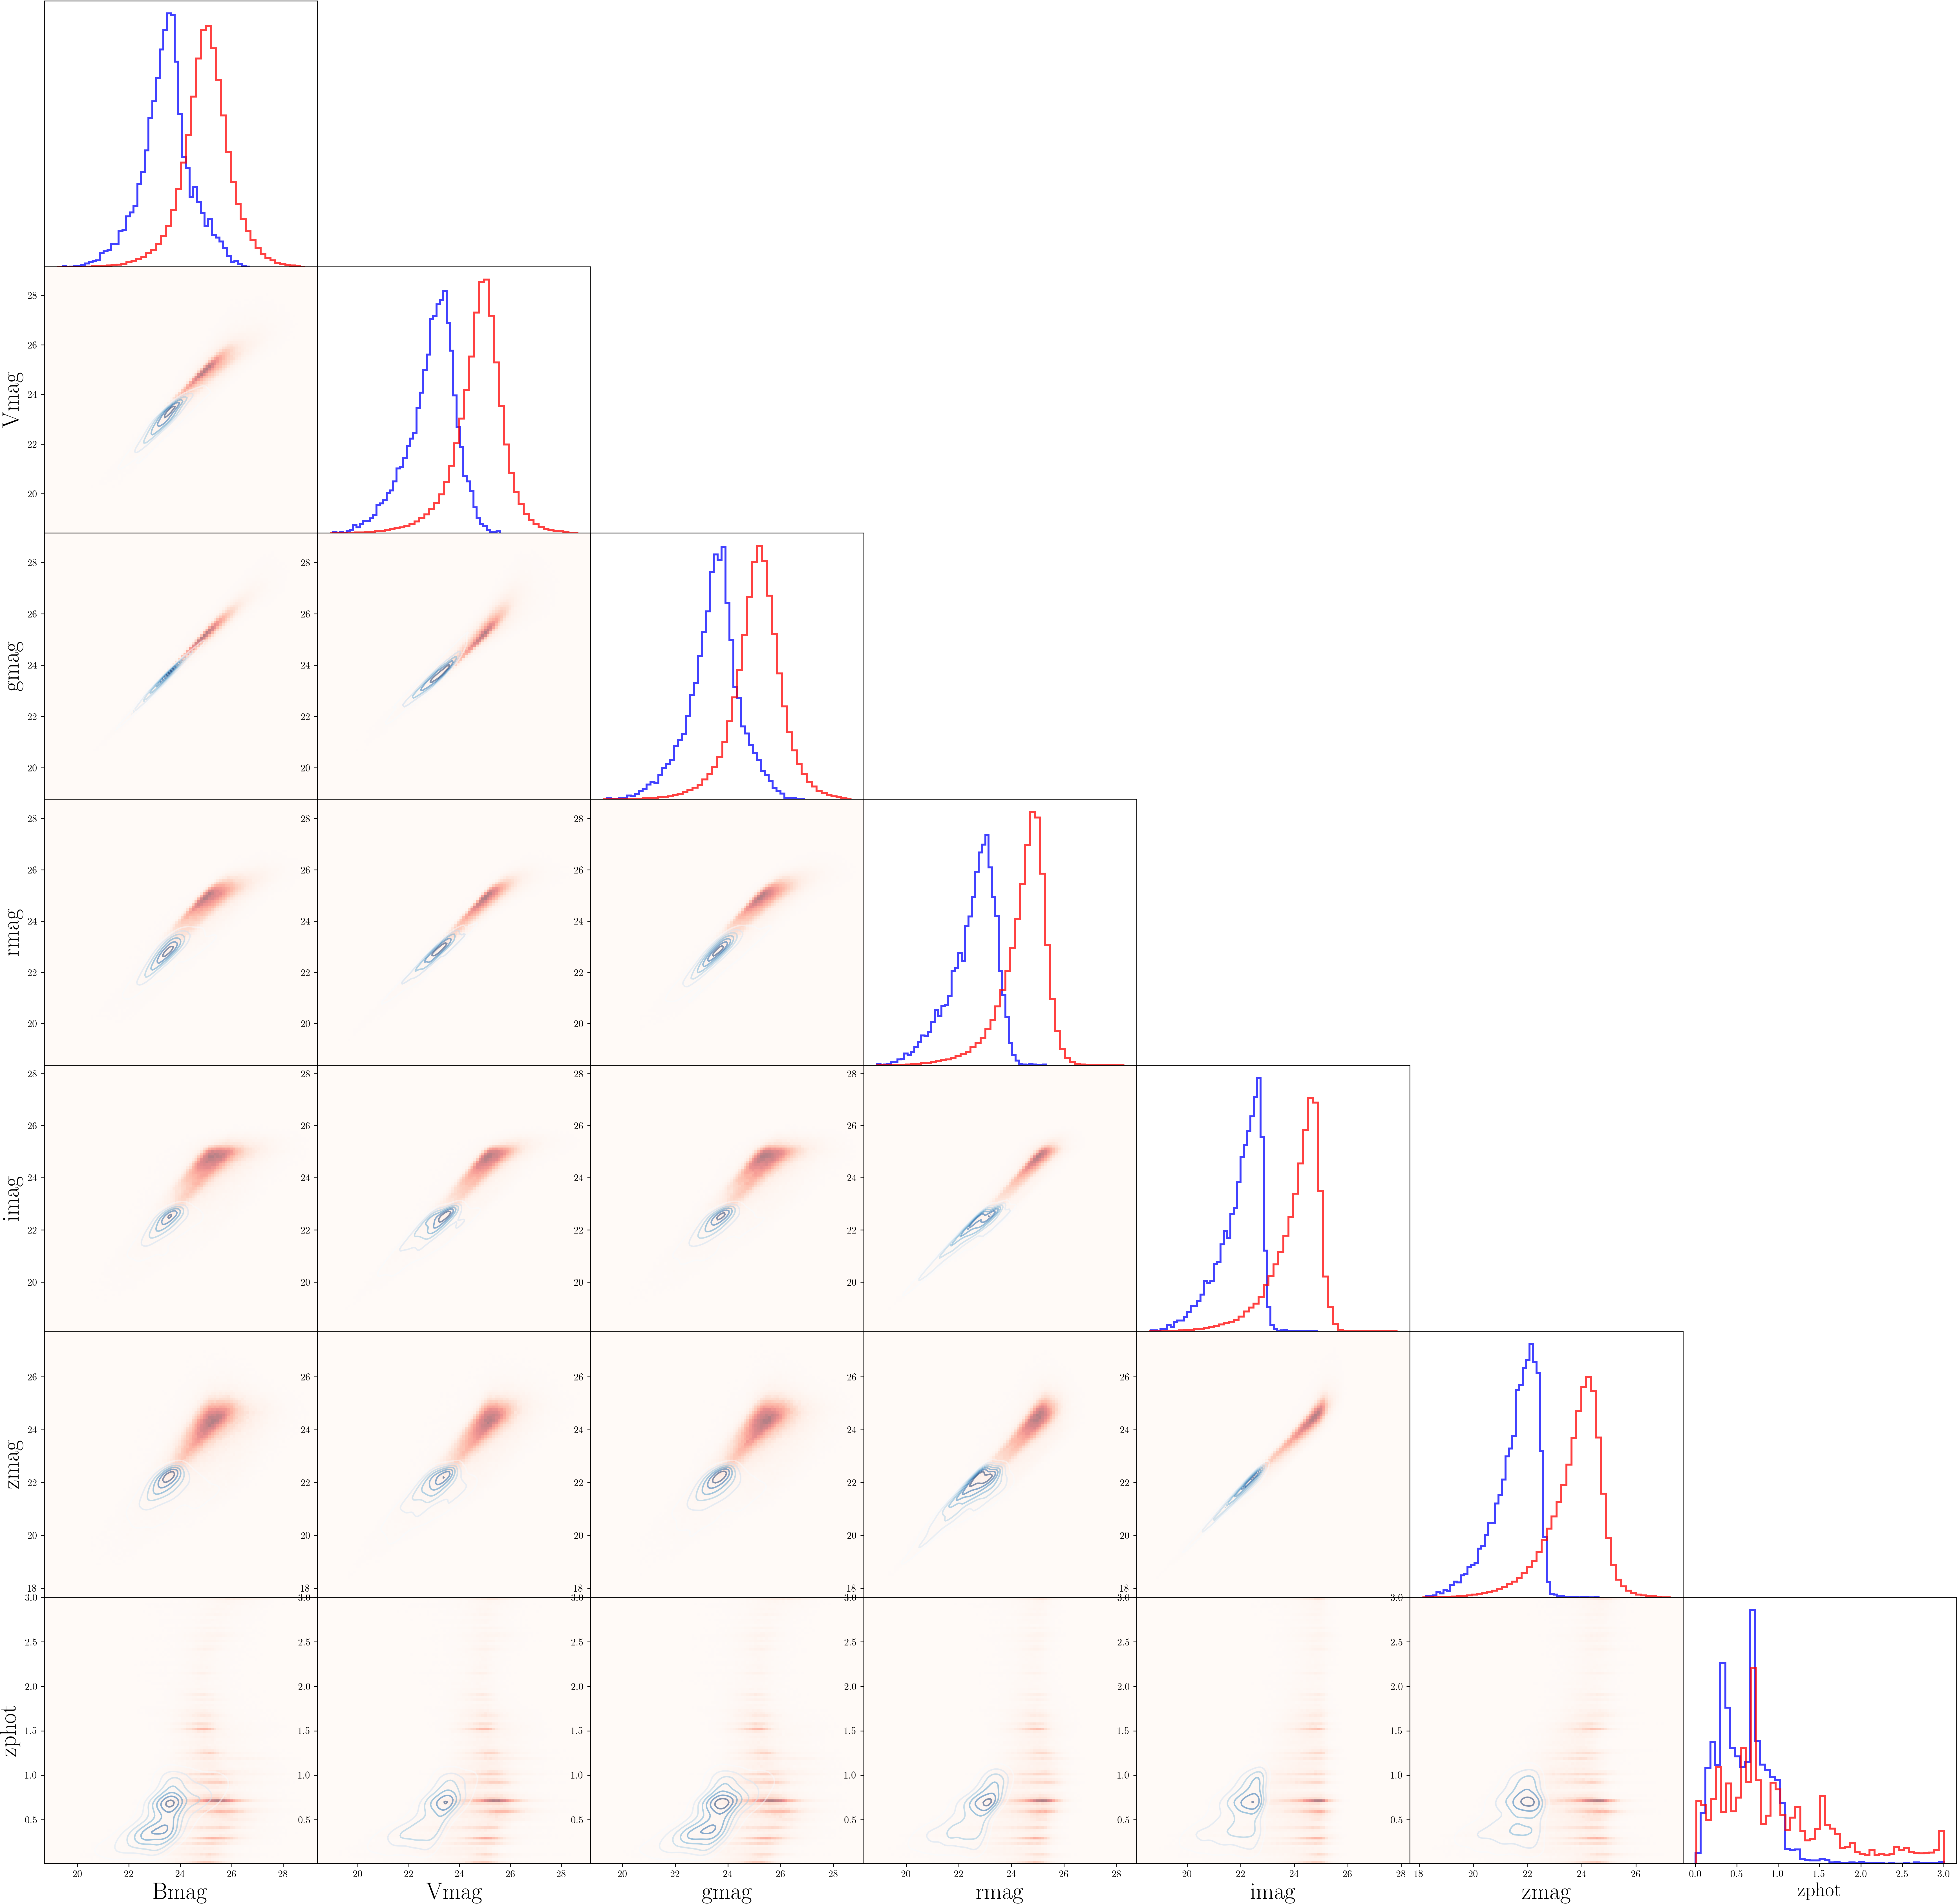
\includegraphics[width=0.99\textwidth]{figures/intro/big_corner_coarse.png}
		\caption{
			The distributions of magnitudes and the provided photometric redshift estimate for the galaxies with complete photometric data in \project{zCOSMOS} ($8,826$ galaxies; blue) and \project{COSMOS} ($395,019$ galaxies; red).
			It is evident that the sample for which spectra were unavailable is not well-supported by the sample for which spectra were obtained, which was used to calibrate the spectroscopically unconfirmed set.
		}
		\figlabel{fig:selection-bias}
	\end{center}
\end{figure*}

%Several factors contribute to photometric redshifts' intrinsic scatter.  
%Distant galaxies are dimmer compared to galaxies of identical luminosity that are closer, driving up photometric errors in flux-limited surveys.  
%The nature of the galaxy sample at higher redshifts also changes, meaning the generation of the photometric redshift posterior based on an a locally-calibrated SED template library or spectroscopically-confirmed training set is more likely to be inappropriate, leading to broader features.  
%In general, the galaxies that could not have been observed spectroscopically will have different and noisier photo-$z$ likelihoods than those that could fall into a spectroscopic training set (or spectroscopically derived template library).  
%This effect may be stronger for high-redshift galaxies.  

Once propagated through the calculations of correlation functions of cosmic shear and galaxy positions, these sources of \pz\ errors are not insignificant contributors to the total uncertainties reported on cosmological parameters.
As other systematic errors have been resolved, the uncertainties associated with \pz s have come to dominate the uncertainties on estimates of cosmological parameters made by current surveys such as \des \citep{hoyle_dark_2017}.

Much effort has been dedicated to improving \pz s, though they are still most commonly obtained by a maximum likelihood estimator (MLE) based on libraries of galaxy SED templates, with conservative approaches to error estimation.  
Recent advances have focused on identifying and removing catastrophic outliers when using \pz s for 
inference \citep{Gorecki2014}.  
Sophisticated Bayesian techniques and cutting-edge machine learning methods have been employed to improve precision \citep{Carliles2010} and accuracy \citep{Sadeh2015}. 

An alternative to point estimation of \pz s is redshift probability distribution function (PDF) estimation that reports the probability $p(z)$ over all possible redshifts for every galaxy rather than an MLE (with or without presumed Gaussian error bars) \citep{Koo1999}.  
This option is favorable because it contains more potentially useful information about the uncertainty on each galaxy's redshift than a point estimate, incorporating notions of precision, accuracy, and systematic errors.
However, denoting \pzpdf s as ``$\pr{z}$'' is an abuse of notation, as it does not adequately convey what information is being used to constrain the redshift $z$; \pzpdf s are \textit{posterior} PDFs, conditioned on the photometric data and prior knowledge, as is covered in detail in \Chap{pedant}, as well as \Chap{chippr} and \Chap{pzdc1}.

\aim{what interesting problems/opportunities are the context for my work?  (drawing conclusions about the universe from vast quantities of uncertainty-dominated, limitations of photometry lead to methodological challenges, what was tried so far and why isn't it good enough)}

\aim{what science can be done with that opportunity? (cosmology, and then some! the interesting problems are in testing LCDM, GR, inflation, also galaxy evolution)}

\Pzpdf s have been produced by completed surveys \citep{Hildebrandt2012, Sheldon2012} and will be produced by ongoing and upcoming surveys \citep{LSSTScienceCollaboration2009, CarrascoKind2014a, Bonnett2015, Masters2015}.  
\Pzpdf s are not without their own weaknesses, however, including the resources necessary to calculate and record them for large galaxy surveys \citep{CarrascoKind2014} and the method used to derive them.  
The most important of these issues, however, is that use of them in the literature is inconsistent at best and incorrect at worst.  
The most common application of \pzpdf s is their use in estimating \Nz, the distribution of redshifts of a sample of galaxies, a quantity essential to the calculation of the power spectra of weak gravitational lensing and large-scale structure that are used to constrain the parameters of cosmological models.
\aim{Provide equations/citations for the use of \Nz\ in cosmology.}

If the true redshifts $\{z_{j'}\}$ were known, the redshift probabilities would be delta functions $\{\delta(z, z'_{j})\}$ centered at the true redshift, and the redshift distribution could be approximated by a histogram or other interpolation of the delta functions $\{\delta(z, z'_{j})\}$.
When \pzpdf s are available instead of true redshifts, the simplest approach reduces them to point estimates of redshift by using $\delta(z, \hat{z}_{j})$ in place of $\delta(z, z'_{j})$, where $\hat{z}_{j}$ may be the mode (maximum) of the \pzpdf, though there are other, more principled options \citep{tanaka_photometric_2018-1}.
However, it is more common at this point to calculate the mathematically invalid but conceptually simple \textit{stacked estimator} of the redshift density function \citep{Lima2008}, 
\begin{align}
\eqlabel{eqn:stack}
\hat{n}(z) &= \frac{1}{\ntot} \sum_{i = 0}^{\ntot} \pr{z_{i}}
\end{align}
for a sample of $\ntot$ galaxies $i$, or, equivalently, the redshift distribution function $\hat{N}(z) = \ntot \hat{n}(z)$.

In \Chap{pedant}, I address the question of how a blatantly incorrect estimator of the redshift distribution could become widely accepted by otherwise clever astrophysicists.
I approach the problem from a mathematically rigorous perspective to identify the assumptions necessary for the stacked estimator to approach the true \Nz and note that because those assumptions will not hold for future surveys, including \lsst, we must use an alternative estimator that self-consistently propagates redshift uncertainty.

I go on to present one such an alternative to stacking, the Cosmological Hierarchical Inference with Probabilistic Photometric Redshifts (\Chippr), in \Chap{chippr}.
\Chippr\ is a probabilistic graphical model (PGM) that encapsulates the causal relationships between the redshift distribution, samples of individual galaxy redshifts, and photometric data.
I also present the \chippr\ code that implements the \Chippr\ model and includes a comprehensive suite of tools for testing arbitrarily realistic mock \pzpdf\ catalogs.

\aim{Hogg says ``I think it would be good to talk a little quantitatively about where people need to know N(z) and other one-point statistics, and how much they will get various things wrong if they don't know these correctly. 
	And situate that discussion within the current context of cosmological parameter estimation and precision cosmology.''}

In order for the approach proposed in \Chap{chippr} to be applied, there must be a \pzpdf\ catalog, yet many techniques to obtain \pzpdf s have been proposed and tested in the literature without clear indications that one is superior to all others.  
An extension of the Bayesian photometric redshift (BPZ) method of \citet{Benitez2000} that produces posterior probability distributions (as opposed to a selection of local maxima) from an SED template library has been employed \citep{Hildebrandt2012, Kelly2014, Lopez-Sanjuan2015}.  
\Pzpdf s have also been obtained by a variety of trustworthy data-driven approaches in the literature: $k$-nearest neighbor algorithms with \citep{Ball2008} and without \citep{Sheldon2012} inclusion of photometric measurement errors, neural networks \citep{Bonnett2015a}, self-organizing maps \citep{CarrascoKind2014a}, and prediction tree and random forest classification techniques \citep{Carliles2010, CarrascoKind2013}.  
(The approaches of fitting to a training set and fitting to a template library are related to one another by \citet{Budavari2009}.)  
Hierarchical inference has also been applied to calculate \pzpdf s simultaneously with the overall redshift distribution function \citep{Leistedt2016}.  
Of course, this brief review does not cover all ways to obtain \pzpdf s; many more may be found in the literature, along with comparisons thereof \citep{Hildebrandt2010, Dahlen2013, Sanchez2013, Bonnett2015}.
Some current work aims to vet \pzpdf\ generation methods \citep{Wittman2016}.
\aim{Also cite the HSC comparison of \pzpdf\ methods, and maybe the DES one even though it only compares two.}
\Chap{pzdc1} details the comparative study of Schmidt, Malz, and Soo, et al. (in review) but goes beyond the scope of previous attempts to identify the best \pzpdf\ technique by critiquing the evaluation criteria themselves from a mathematically rigorous perspective.
\aim{Make this a real citation with a link to the paper.}

In the absence of an obvious best choice for the method used to derive \pzpdf s, \lsst\ has planned to provide \pzpdf s obtained by a number of promising methods rather than choosing one, effectively hedging their bets on which may ultimately prevail.
This goal of storing multiple \pzpdf s, however, must be accomplished without exceeding the available data storage capacity of the survey nor compromising the integrity of subsequent science applications due to loss of information in the compression and reconstruction schemes.
\Chap{qp} approaches the problem of choosing how best to store \pzpdf s such that the results of multiple \pzpdf\ techniques may be available to the scientific community, focusing in particular on the number of stored parameters under different possible parameterizations of stored \pzpdf s.

\aim{Update this paragraph for the existence of \Chap{pedant}.}
\Chap{chippr} presents a mathematically rigorous methodology for inferring \Nz\ from a catalog of \pzpdf s, including the effect of incorrectly inferred \Nz\ on cosmological parameter estimates.
\Chap{pzdc1} contains a comprehensive comparison of twelve approaches to probabilistic photometric redshift estimation, presenting novel discoveries of the impact of the assumptions implicit to the method by which the redshift probabilities are derived and the limitations of established performance metrics of such probabilistic data products in assessing the quality of the procedures for deriving them.
I also address in \Chap{qp} a practical concern regarding how redshift probabilities are to actually be used, answering the question of how probabilistic data products should be stored and delivered to users in order to ensure that scientific progress can be made, as well as how to go about answering that question for a generic science application.

\aim{did I produce anything of value? if there's a product, maybe cite it here?}

\chapname~\chapalt{chippr} has been presented at numerous conferences but remains an unpublished, public draft accompanied by a public code.
\chapname~\chapalt{pzdc1} is currently under \desc\ internal review, with intended submission to MNRAS.
\chapname~\chapalt{qp} has been refereed and published in AJ, with code published on Zenodo.
Here, I describe my specific contributions to each \chapname and acknowledge the contributions of my co-authors:
\begin{enumerate}

{\item For \chap{chippr}, I led the development, implementation, and validation of CHIPPR initially under the supervision of David Hogg (NYU) and later continued to work on all three aspects of the project under the supervision of Phil Marshall (SLAC).
	I developed the mathematical formalism in consultation with Phil Marshall (SLAC).}

{\item For \chap{pzdc1}, I led the choice, evaluation, and interpretation of the comparison metrics, and I devised and implemented the \texttt{trainZ} technique of \pzpdf\ estimation.
	I wrote the paper in collaboration with Sam Schmidt (UC Davis), John Soo (U. of Science Malaysia), and the \Pz\ Working Group of the \desc.  
	The mock data was produced and validated by Alex Abate (Dia\&Co), Sam Schmidt (UC Davis), Eve Kovacs (Argonne), Joe DeRose (Stanford), Risa Wechsler (Stanford), Tina Peters (Toronto).
	The experimental design was chosen by Ofer Lahav (UCL), Jeff Newman (Pitt), Sam Schmidt (UC Davis), and Tony Tyson (UC Davis).
	I chose the metrics to test with input from Jeff Newman (Pitt) and Ann Lee (CMU).
	I worked together with Rongpu Zhou (Pitt), Bryce Kalmbach (UW), Kartik Iyer (Rutgers), Sam Schmidt (UC Davis), and Chris Morrison (UW) to implement the comparison metrics and run them on the results of different \pzpdf\ codes.
	The \pzpdf\ codes themselves were written and/or run by Ibrahim Almosallam (King Abdulaziz City for Science and Technology), Massimo Brescia (INAF-Capodimonte), Stefano Cavuoti (University Federico II), Johann Cohen-Tanugi (Universit\'e de Montpellier),  Andy Connolly (UW), Peter Freeman (CMU), Melissa Graham (UW), Rafael Izbicki (Federal University of Sao Carlos), Matt Jarvis (Oxford; University of the Western Cape), Ann Lee (CMU), Giuseppe Longo (University Federico II), Erfan Nourbakhsh (UC Davis), Eric Nuss (Universit\'e de Montpellier), Taylor Pospisil (CMU), Cecile Roucelle (U Clermont-Ferrand), and Hugo Tranin (Universit\'e de Montpellier).
	The paper is intended for submission to MNRAS but is still under internal review by \desc\ members Mike Troxel (Duke), Markus Michael Rau (CMU), and Daniel Gruen (Stanford).}

{\item For \chap{qp}, I devised the idea for the project, conducted the investigation, wrote and validated the \texttt{qp} code, and wrote the paper under the supervision of Phil Marshall (SLAC), with contributions to the mock data production by Sam Schmidt (UC Davis), Melissa Graham (UW), Joe DeRose (Stanford), and Risa Wechsler (Stanford).
	The paper was internally reviewed by \desc\ members Chad Schafer (CMU), Boris Leistedt (NYU), and Chris Morrison (UW).}

\end{enumerate}


%\renewcommand{\chapid}{chapter}

% Chapter specific commands:
\newcommand{\thisplain}{[insert repo name]}
\newcommand{\this}{\project{\thisplain}}
\newcommand{\license}{MIT License}
\newcommand{\Python}{\project{Python}}
\newcommand{\numpy}{\project{numpy}}
\newcommand{\Ubuntu}{\project{Ubuntu}}
\newcommand{\github}{\project{GitHub}}
\newcommand{\pip}{\project{pip}}
\newcommand{\acor}{\project{acor}}
\defcitealias{Goodman:2010}{GW10}

% Math:
\newcommand{\model}{\ensuremath{\vector{\Theta}}}
\newcommand{\data}{\ensuremath{\vector{D}}}
\newcommand{\nuisance}{\ensuremath{\vector{\alpha}}}
\newcommand{\link}{\ensuremath{X}}
\newcommand{\ensemble}{S}
\newcommand{\colorens}[1]{\ensemble^{(#1)}}
\newcommand{\red}{\colorens{0}}
\newcommand{\blue}{\colorens{1}}
\renewcommand{\vector}[1]{#1}
\renewcommand{\matrix}[1]{#1}

\chapter{[Title of Chapter]\chaplabel{chapter}}

This \paper\ represents joint work with [people] published in [place] as [citation].

\section{Chapter abstract}

[probably the paper abstract]

\section{Introduction}

[probably the paper intro, and then all the other sections from the paper]

\section{[Sections]}

[expand those sections into subsections to give all the thorough background content that belongs in a thesis but not in a paper]

\section{Chapter acknowledgements}

It is a pleasure to thank
[helpful people here]
for helpful contributions to the ideas and code presented here.

\renewcommand{\chapid}{chippr}

% Chapter specific commands:
\newcommand{\cosmolike}{\repo{CosmoLike}}
\newcommand{\emcee}{\repo{emcee}}
\newcommand{\boss}{\project{BOSS}}
\newcommand{\mmle}{marginalized maximum likelihood estimate}% really marginalized maximum a posteriori estimate, may still change this

% rules for my math notation, in case I get confused
% galaxies i, redshifts j, combinations k
% N galaxies out of N_tot galaxies
% dagger for "truth", tilde for interim, prime for proposed/different
% prior info I_[informative subscript]

\chapter{ How to obtain the redshift distribution from probabilistic redshift estimates \chaplabel{chippr} }

This \paper\ was incubated with David Hogg (NYU) during the summer and fall of 2015 and has been publicly available on \github\footnote{\url{https://github.com/aimalz/chippr}} since its inception.
I further developed the code and refined the scope with Phil Marshall (SLAC) in the spring and fall of 2017.

\section*{Chapter abstract}

A trustworthy estimate of the redshift distribution \nz\ is crucial for using galaxy catalogs to study cosmology via weak gravitational lensing and large-scale structure.
Spectroscopic redshifts for the dim and numerous galaxies of weak-lensing surveys are expected to be inaccessible, making photometric redshifts (photo-$z$s) the next-best alternative.
The nontrivial systematics affecting photo-$z$ estimation have motivated the weak-lensing community to favor photo-$z$ probability density functions (PDFs) as a more comprehensive alternative to photo-$z$ point estimates.
However, analytic methods for utilizing these new data products in cosmological inference are still evolving.
The ubiquitous methodology known as stacking produces a systematically biased estimator of $n(z)$ that worsens with decreasing signal-to-noise, the very regime where photo-$z$ PDFs are most necessary.
We introduce a mathematically rigorous probabilistic graphical model (PGM) of hierarchical inference of $n(z)$, which is provably the only self-consistent way to combine photo-$z$ PDFs to produce an estimator of $n(z)$.
The novel Cosmological Hierarchical Inference with Probabilistic Photometric Redshifts (\Chippr) model yields a more accurate characterization of $n(z)$ by correctly propagating the redshift uncertainty information beyond the best-fit estimator produced by traditional procedures.
We conclude by propagating these effects to constraints in the space of cosmological parameters.

\section{Introduction}
\sectlabel{sec:intro}

Though their potential to improve estimates of physical parameters is tremendous, \pzpdf s have been applied only to a limited extent.  
They have been used to form selection criteria of samples from galaxy surveys without propagation 
through the calculations of physical parameters \citep{VanBreukelen2009,Viironen2015}.  
Probability cuts on Bayesian quantities are not uncommon \citep{Leung2015, DiPompeo2015a}, but that procedure does not fully take advantage of all information contained in a probability distribution for parameter inference.  

Despite the growing prevalence of \pzpdf\ production, no implementation of inference using \pzpdf s has yet been presented with a mathematically consistent methodology.  
I present and validate a hierarchical Bayesian technique for the use of \pzpdf\ in inference of arbitrary statistics relevant to cosmology, large-scale structure, and galaxy evolution.  
For simplicity, we consider only one-point statistics, though future work will extend this methodology to higher-order statistics.

The \textit{redshift distribution function \Nz}, or, almost interchangably, its normalized cousin the \textit{redshift density function \nz}, serves as an ideal statistic upon which to demonstrate this novel approach.  
\Nz\ is necessary for calculations of two-point correlation functions of weak gravitational lensing and counting statistics that are used to probe dark energy \citep{Masters2015}.  
The observed \Nz\ also been used to validate survey selection functions used in generation of realistic, multi-purpose mock catalogs \citep{Norberg2002}.  
Additionally, \Nz\ has been the subject of inference using \pzpdf s before \citep{Sheldon2012, Hildebrandt2012, Kelly2014, Benjamin2013, Bonnett2015a, Viironen2015, Asorey2016, Leistedt2016}, so comparisons to the literature may easily be made. 

The prevailing way to estimate \nz\ for a sample of $N_{tot}$ galaxies $i$ is to ``stack'' \pzpdf s according to
\begin{align}
\eqlabel{eqn:stack}
\hat{n}(z) &= \frac{1}{\ntot} \sum_{i = 0}^{\ntot} \pr{z_{i}} .
\end{align}
The stacked estimator of the redshift density function is effectively an average of the \pzpdf\ catalog and, as I will show in this \paper, not in general mathematically valid.
Stacking is considered the preferred method for obtaining \Nz\ from a dataset of interim photo-$z$ posteriors \citep{Sheldon2012, Kelly2014, Benjamin2013, Bonnett2015a, Viironen2015, Asorey2016}.  
However, it must be noted here that \Eq{eqn:stack} is not in general mathematically valid.  
(See \citet{Hogg2012} for a complete discussion.)  
The estimator produced by stacking shall henceforth be referred to as the ``stacked'' estimator.

\aim{Motivate how well we need to know \Nz\ and why it matters.
	New paragraph here: Say what precision is needed for \Nz\ for future weak lensing surveys. 
	Say what precision the mass function is needed (in, say cluster studies) for precision cosmology.}

I aim to develop a clear methodology guiding the use of \pzpdf s in inference so they may be utilized effectively by the cosmology community.

In \Sect{sec:meth}, I present the \Chippr\ model and \chippr\ implementation for characterizing the full posterior probability landscape of \Nz\ using \pzpdf s. 
In \Sect{sec:alldata}, I describe the experimental design for testing the fully probabilistic approach to mock and real datasets, the results of which are found in \Sect{sec:results}.
In \Sect{sec:results}, I stress-test the \Chippr\ model against stacking and its other competitors in the context of cosmology.

\section{Method}
\sectlabel{sec:meth}

\aim{Q: How can we improve the effectiveness of using \pzpdf s in inference?\\
	A: Hierarchical inference is the only self-consistent way.}

Consider a survey of $J$ galaxies $j$, each with photometric data $\data_{j}$; thus the entire survey over some solid angle produces the ensemble of photometric magnitudes (or colors) and their associated observational errors $\{\data_{j}\}$.  
Each galaxy $j$ has a redshift $z_{j}$ that we would like to learn; redshift is a parameter in this case.  
The distribution of the ensemble of redshifts $\{z_{j}\}$ may be described by the hyperparameters defining the redshift distribution function \nz\ that we would like to quantify.  
This situation may be considered to be a probabilistic generative model, illustrated by the directed acyclic graph of \Fig{fig:pgm}.  

The redshift distribution function \nz\ is the number of galaxies per unit redshift, effectively defining the evolution in the number of galaxies \citep{Menard2013}.  
In the following sections, I present and compare methods for estimating \nz\ from \pzpdf s.  
\Sect{sec:prob} contains the mathematical derivation of a probabilistic model for $n(z)$ dependent on photo-$z$ probability distribution functions, and \Sect{sec:sheldon} contrasts the probabilistic model with alternative methods.

\subsection{Forward Model}
\sectlabel{sec:forward}

We begin by reframing the redshift distribution \nz\ from a probabilistic perspective.
Here we define a redshift density \nz\ as the normalized probability density
\begin{equation}
\eqlabel{eqn:nz}
\int_{-\infty}^{\infty}\ n(z)\ dz\ \equiv\ \frac{1}{J}\ \int_{-\infty}^{\infty}\ \sum_{j=1}^{J}\ \delta(z_{j},\ z)\ dz = 1
\end{equation}
of finding a galaxy $j$ in a catalog of $J$ galaxies having a redshift $z$.
\aim{Fix font or limits in \Eq{eqn:nz}.}
We believe that galaxy redshifts are indeed drawn from \nz, making it a probability density over redshift; this fact can also be confirmed by dimensional analysis of \Eq{eqn:nz}.
\aim{Cite Hogg's probability calculus for inference document.}

We may without loss of generality impose a parameterization
\begin{equation}
\eqlabel{eqn:fz}
f(z; \ndphi)\ \equiv\ n(z)
\end{equation}
in terms of some parameter vector $\ndphi$.
At this point, the parameter vector is quite general and may represent coefficients in a high-order polynomial as a function of redshift, a set of means and variances defining Gaussians that sum to the desired distribution, a set of histogram heights that describe a binned version of the redshift distribution function, etc.
Upon doing so, we may rewrite \Eq{eqn:fz} as 
\begin{equation}
\eqlabel{eqn:pz}
z_{j}\ \sim\ \pr{z \gvn \ndphi}\ \equiv\ f(z; \ndphi),
\end{equation}
a probability density over redshift conditioned on the parameters $\ndphi$ specifying \nz.
Note that $z_{j}$ does not depend on the redshift $z_{j'}$ of some other galaxy $j' \neq j$, a statement of the causal independence of galaxy redshifts from one another.

In addition to believing \nz\ is a PDF from which redshifts are drawn, we also believe that there is some higher dimensional probability space $\pr{z, \data}$ of redshift and photometric data vectors $\data$, which may be any combination of fluxes, magnitudes, colors, and their observational errors.
In that sense \nz\ is equivalent to an integral
\begin{equation}
\eqlabel{eqn:integral}
n(z)\ =\ \integral{\pr{z, \data}}{\data}
\end{equation}
over the dimension of data in that joint probability space.
Note that galaxies may have different observational data despite sharing the same redshift, and that galaxies at different redshifts may have identical photometry; the space $\pr{z, \data}$ need not be one-to-one.
We assume a stronger version of statistical independence here, that draws $(z_{j}, \data_{j})$ are independent of draws $(z_{j'}, \data_{j'})$ in this space; the data and redshift of each galaxy are independent of those of other galaxies.

However, this problem has additional causal structure that we can acknowledge.
The photometry results from the redshifts, not the other way around.
This is the fundamental assumption upon which \pz\ estimation is based.
The forward model corresponds to first drawing redshifts according to \Eq{eqn:pz} and then drawing data from the likelihood
\begin{equation}
\eqlabel{eqn:pzpdf}
\data_{j}\ \sim\ \pr{\data \gvn z_{j}}
\end{equation}
of photometry conditioned on redshift, illustrated in \Fig{fig:pedagogical_scatter}.
\aim{Describe joint space of true and ``observed'' redshift as a special nonlinear projection of the data}
The likelihoods can be thought of as cuts through the joint probability space of redshift and photometry, evaluated at the true redshifts.

\begin{figure*}
	\begin{center}
		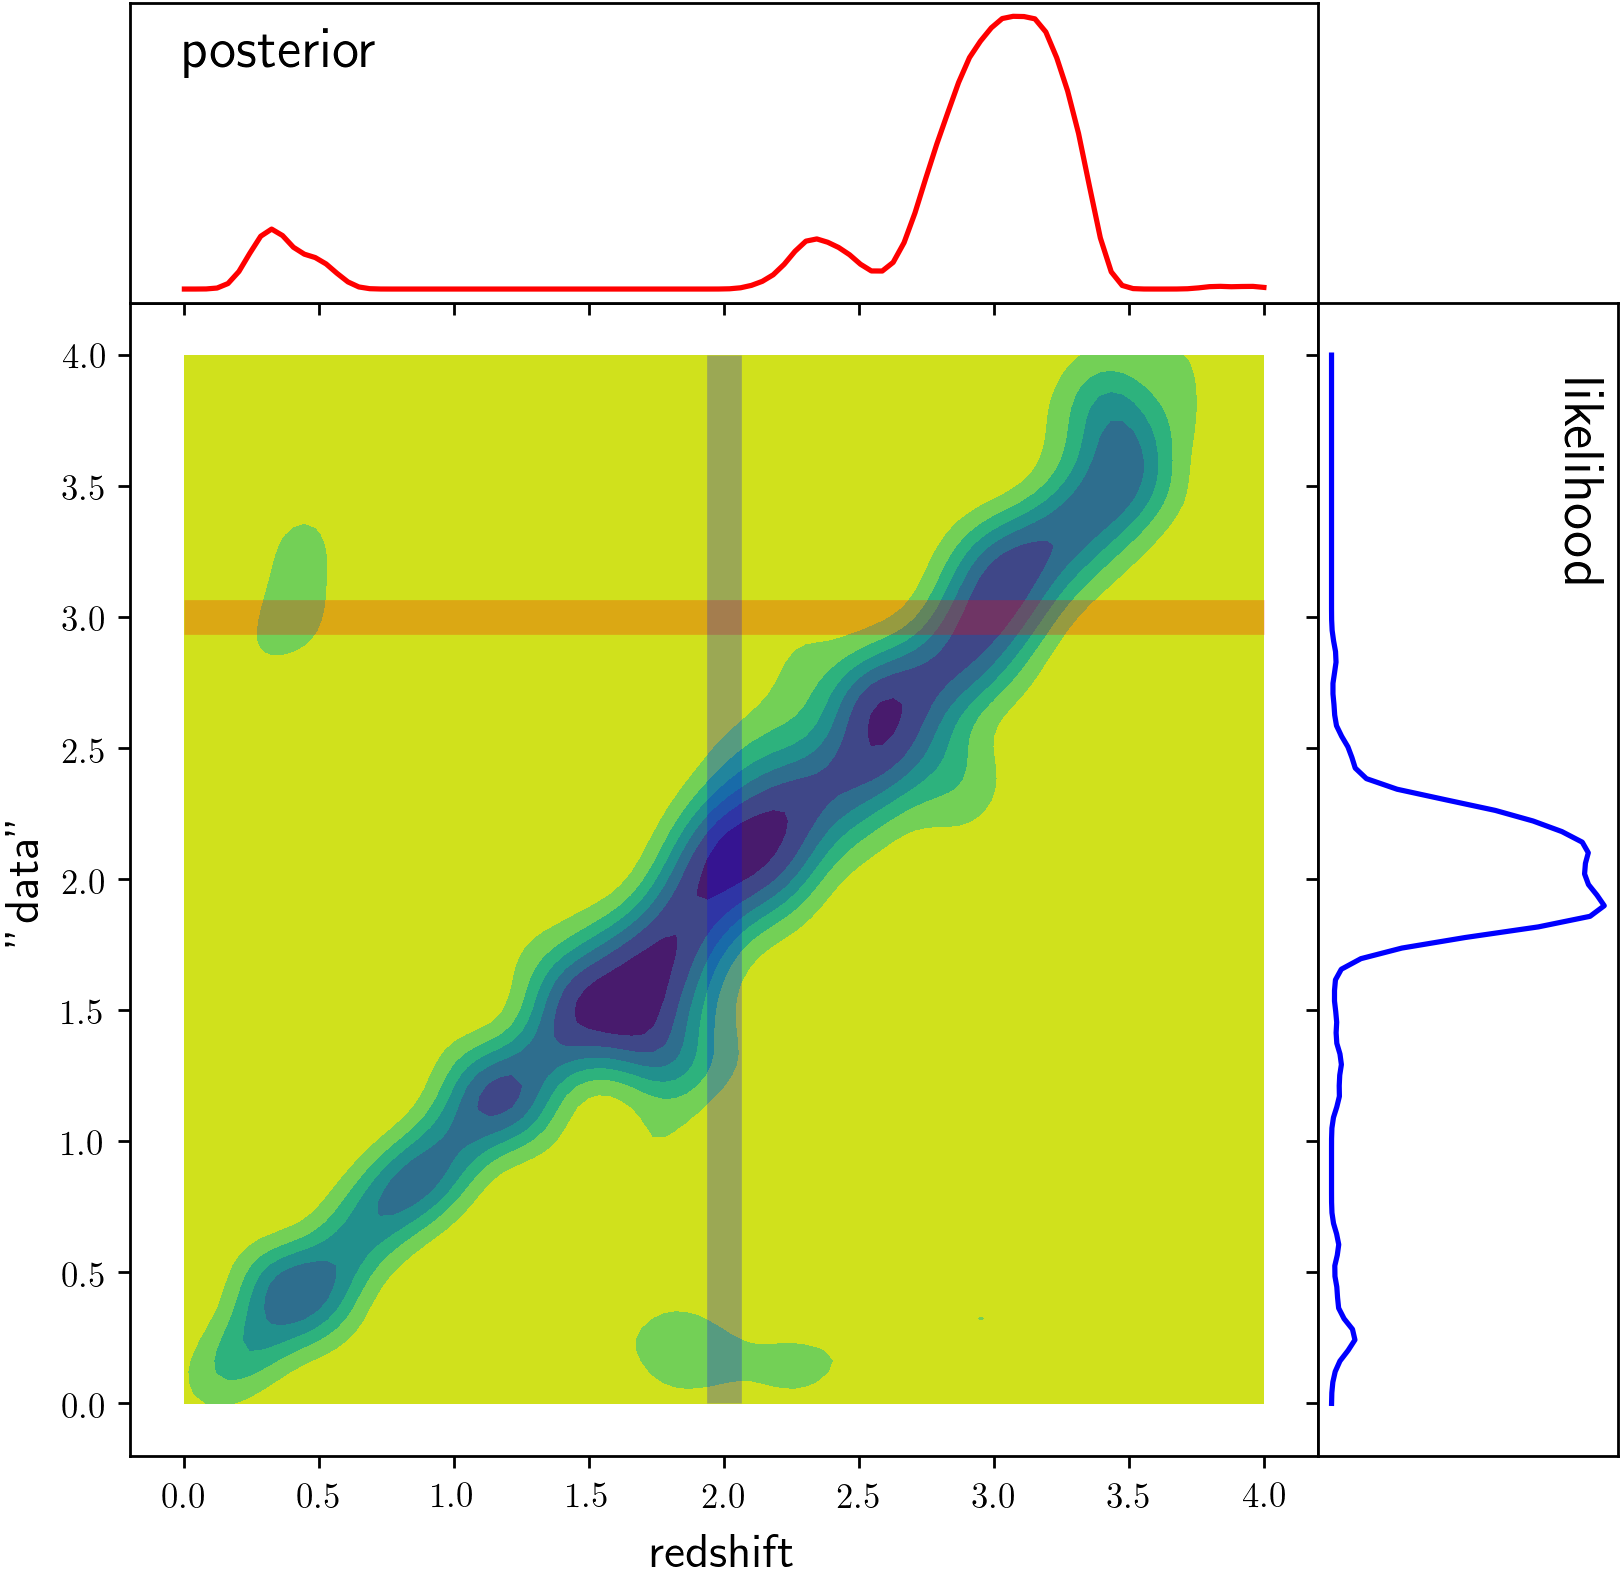
\includegraphics[width=\textwidth]{figures/chippr/jain05.png}
		\caption{
			\aim{Cite Jain+05, WebPlotDigitizer for inspiring this figure.}
			A generic probability space of redshift (x-axis) and data (y-axis), projected into a single dimension, with vertical cuts and marginals (cyan) indicating the construction of likelihoods and horizontal cuts and marginals (magenta) indicating the construction of posteriors.
			\aim{Choose better colors?}
		}
		\figlabel{fig:pedagogical_scatter}
	\end{center}
\end{figure*}

This description of the physical system corresponds to a forward model by which we actually believe photometry is generated:
\begin{enumerate}
	\item There exists a redshift distribution \nz\ with parameters $\ndphi$.
	\item Galaxy redshifts $\{z_{j}\}$ are independent draws from $\pr{z \gvn \ndphi}$.
	\item Galaxy photometry $\data_{j}$ is drawn from the likelihoods $\pr{\data_{j} \gvn z}$.
\end{enumerate}

\subsection{Probabilistic Model}
\sectlabel{sec:prob}

A forward model such as that of \Sect{sec:forward} corresponds to a probabilistic graphical model (PGM), represented by a directed acyclic graph (DAG) as in \Fig{fig:pgm}.
A DAG conveys the causal relationships between physical parameters and, like a Feynman diagram in the context of particle physics, is a shorthand for mathematical relationships between variables.
The photometric data $\data_{j}$ of a galaxy is drawn from some function of its redshift $z_{j}$, independent of other galaxies' data and redshift.
Both data and redshift are random variables, but data is the one that we observe and redshift is not directly observable.
In this problem, we don't care about further constraining the redshifts of individual galaxies, only the redshift distribution, so we consider redshift to be a \textit{latent variable}.
Because the parameters $\ndphi$ that we seek are causally separated from the data by the latent variable of redshift, we call them \textit{hyperparameters}.
\aim{I'm not explaining the distinction between hyperparameters and parameters adequately.}

\begin{figure}
	\begin{center}
		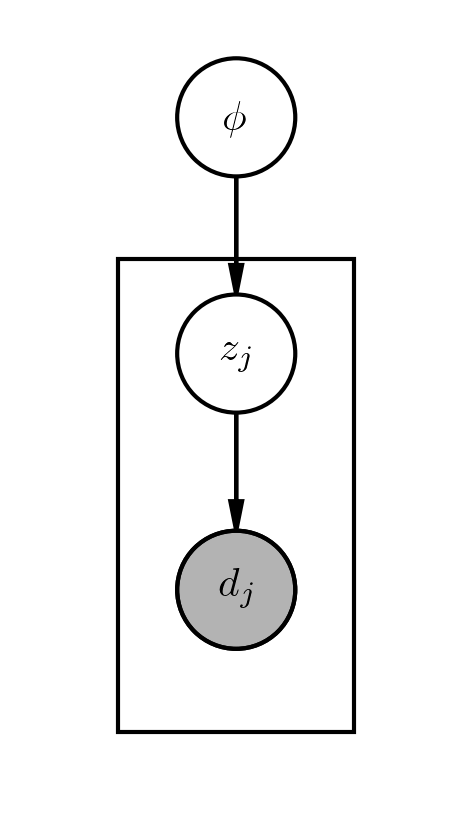
\includegraphics[width=0.25\textwidth]{figures/chippr/pgm.png}
		\caption{The directed acyclic graph of the CHIPPR model, where circles indicate random variables and arrows indicate causal relationships.
			The redshift distribution function parameterized by hyperparameters $\ndphi$ exists independent of the survey of $J$ galaxies, indicated as a box.  
			The redshifts $\{z_{j}\}$ of all galaxies in the survey are latent variables independently drawn from the redshift distribution, which is a function of $\ndphi$. 
			The photometric data $\data_{j}$ for each galaxy is drawn from a function of its redshift $z_{j}$ and observed, indicated by a shaded circle.}
		\figlabel{fig:pgm}
	\end{center}
\end{figure}

The problem facing cosmologists is to determine the true value of $\ndphi$ from observing the photometry $\{\data_{j}\}$ of a large sample of $J$ galaxies $j$.
To self-consistently propagate the uncertainty in the redshifts, however, it is more appropriate to estimate the posterior $\pr{\ndphi \gvn \{\data_{j}\}}$ over all possible values of $\ndphi$ conditioned on all the observed data $\{\data_{j}\}$ available in a generic catalog.
In order to use the DAG of \Fig{fig:pgm} to derive an expression for $\pr{\ndphi \gvn \{\data_{j}\}}$ in terms of \pzpdf s, we must introduce two more concepts, confusingly named the implicit prior and the prior probability density.

When we constrain the redshift of a galaxy using its observed photometric data $\data_{j}$, we are effectively estimating a posterior $\pr{z \gvn \data_{j}}$.
However, to do this, we must have a model for the general relationship between redshifts and photometry, whether empirical, as is the case for machine learning \pzpdf\ methods, or analytic, as is the case for template-based \pzpdf\ methods.
Such a relationship is defined in the space of probability density over redshift, so it must be able to be parameterized by the same functional form $f(z; \ndphi)$ as \nz .
It is thus natural to write it as $\pr{z \gvn \ndphi^{*}}$, where $\ndphi^{*}$ is the parameters for this relationship under some generic \pzpdf\ method.
We call $\pr{z \gvn \ndphi^{*}}$ the \textit{implicit prior}, as it is rarely explicitly known nor chosen by the researcher; for template-based methods where it can be chosen to be ``realistic,'' it may be appropriate to call it an \textit{interim prior}.
Because the implicit prior is unavoidable, the \pzpdf s reported by any method are really \textit{implicit-weighted posteriors} $\pr{z \gvn \data, \ndphi^{*}}$.

%Posteriors differ from likelihoods by way of a prior distribution, so we cannot simply assume that the available data products are \pz\ posteriors $\pr{z \gvn \data_{j}}$.  
%Rather, we have a catalog of implicit-prior weighted \pz\ posteriors $\pr{z \gvn \data_{j}, \ndphi^{*}}$.  
%There must have been some interim prior probability distribution $p(z|\vec{\theta}^{*})$ defined in terms of the interim prior parameter values (hereafter the interim prior) $\vec{\theta}^{*}$ explicitly chosen or implicitly made to perform the calculation of the probabilistic photo-$z$s.  
%If it is implicit, it may not be representable in the parametrization we have chosen, and furthermore it may not be known at all; a method that produces interim photo-$z$ posteriors of this kind is not suitable for inference.  
%However, so long as the implicit prior is known, hierarchical inference is possible. 

The implicit prior $\ndphi^{*}$ may be thought of as an initial guess for the parameters contained in $\ndphi$, inspired by the generative model for photometry from the redshift distribution functions and including some parameters defining intrinsic galaxy spectra and instrumental effects. 
(See \citealt{Benitez2000} for more detail.)  
For statistical purposes, we would like any interim prior to be uninformative, but this is rarely achievable.  
In the case of estimating \nz\ photometrically, it is common to use $\ndphi^{*}$ corresponding to \nz\ derived from some different, spectroscopically confirmed sample or from a cosmological simulation.

The prior probability density $\pr{\ndphi}$ is a more familiar concept in astronomy; to progress, we will have to choose a prior probability density over all possible parameters $\ndphi$.
This prior need not be excessively proscriptive; for example, it may be chosen to enforce smoothness at physically motivated scales in redshift without imposing any particular region as over- or under-dense.

With these definitions, we obtain the desired expression for $\pr{\ndphi \gvn \{\data_{j}\}}$,
\begin{align}
\begin{split}
\eqlabel{eqn:fullpost}
\pr{\ndphi \gvn \{\data_{j}\}} & \propto \pr{\ndphi}\left[\integral{\prod_{j=1}^{J} \left(\pr{z \gvn \data_{j}, \ndphi^{*}}\pr{z \gvn \ndphi}(\pr{z \gvn \ndphi^{*}})^{-1}\right)}{z}\right] ,
\end{split}
\end{align}
the heart of \Chippr.
The derivation is provided below in \Sect{app:math}.

\subsubsection{Derivation}
\sectlabel{app:math}

%We begin by parametrizing $N(z)$ in terms of $\vec{\theta}$, comprising some set of hyperparameters that define the form $N(z)$ may take in whatever basis we choose.  
%We define a function $f_{\vec{\theta}}(z)=N(z)$ that transforms these hyperparameters into the redshift distribution function $N(z)$.  
%Because 
%\begin{equation}
%\eqlabel{eq:definition}
%N(z) \propto p(z \gvn \vec{\theta}),
%\end{equation}
%we may discontinue discussion of $N(z)$ in favor of the likelihood $p(z|\vec{\theta})$.

In this \paper, we work exclusively with log-probabilities.  
What we wish to estimate is then the full log-posterior probability distribution (hereafter the full log-posterior) of the hyperparameters $\ndphi$ given the catalog of photometry $\{\data_{j}\}$.

By Bayes' Rule, the full log-posterior
\begin{equation}
\eqlabel{eqn:basicbayes}
\ln[\pr{\ndphi \gvn \{\data_{j}\}}] = \ln[\pr{\{\data_{j}\} \gvn \ndphi}] + \ln[\pr{\ndphi}] - \ln[\pr{\{\data_{j}\}}]
\end{equation}
may be expressed in terms of the full log-likelihood probability distribution (hereafter the full log-likelihood) $\ln[\pr{\{\data_{j}\} \gvn \ndphi}]$ by way of a hyperprior log-probability distribution (hereafter the hyperprior) $\ln[\pr{\ndphi}]$ over the hyperparameters and the log-evidence probability of the data $\ln[\pr{\{\data_{j}\}}]$.
However, the evidence is rarely known, so we probe the full log-posterior modulo an unknown constant of proportionality.

The full log-likelihood may be expanded in terms of a marginalization over the redshifts as parameters, as in 
\begin{equation}
\eqlabel{eqn:marginalize}
\ln[\pr{\{\data_{j}\} \gvn \ndphi}] = \ln\left[\integral{\pr{\{\data_{j}\} \gvn \{z_{j}\}} \pr{\{z_{j}\} \gvn \ndphi}}{\{z_{j}\}}\right].
\end{equation}

We shall make two assumptions of independence in order to make the problem tractable; their limitations are be discussed below.  
First, we take $\ln[\pr{\{\data_{j}\} \gvn \{z_{j}\}}]$ to be the sum of $J$ individual log-likelihood distribution functions $\ln[\pr{\data_{j} \gvn z_{j}}]$, as in 
\begin{equation}
\eqlabel{eqn:indiedat}
\ln[\pr{\{\data_{j}\} \gvn \{z_{j}\}}] = \sum_{j=1}^{J}\ \ln[\pr{\data_{j} \gvn z_{j}}],
\end{equation}
a result of the definition of probabilistic independence encoded by the box in \Fig{fig:pgm}.
Second, we shall assume the true redshifts $\{z_{j}\}$ are $J$ independent draws from the true $\pr{z \gvn \ndphi}$.  
Additionally, $J$ itself is a Poisson random variable.  
The combination of these assumptions is given by 
\begin{equation}
\eqlabel{eqn:indie}
\ln[\pr{\{z_{j}\} \gvn \ndphi}] = -\integral{f(z; \ndphi)}{z} + \sum_{j=1}^{J}\ \ln[\pr{z_{j} \gvn \ndphi}].
\end{equation}
%It is important to note that the integral $\integral{n(z)}{z} N(z)\ dz$ is not constrained to equal the variable defining the Poisson distribution but instead $J$ by \Eq{eq:definition}, which can be thought of as another parameter.  
The derivation differs when $J$ is not known, say, when we want to learn about a distribution in nature rather than a distribution specific to data in hand, but for a photometric galaxy catalog where the desired quantity is $n(z)$ for the galaxies entering a larger cosmology calculation, it is a fixed quantity.
A detailed discussion of this matter may be found in \citet{Foreman-Mackey2014}.  
Applying Bayes' Rule, we may combine terms to obtain 
\begin{equation}
\eqlabel{eqn:posterior}
\ln[\pr{\ndphi \gvn \{\data_{j}\}}] \propto \ln[\pr{\ndphi}] - \integral{f(z; \ndphi)}{z} + \sum_{j=1}^{J}\ln\left[\integral{\pr{\data_{j} \gvn z} \pr{z \gvn \ndphi}}{z}\right].
\end{equation}

%\Eq{eq:posterior} contains two quantities that merit further discussion, the prior distribution $p(\vec{\theta})$ discussed further in \Sect{sec:exp} and the photo-$z$ log-likelihoods $\ln[p(\vec{d}_{j}|z_{j})]$ that have not been mentioned since \Eq{eq:marginalize}.  
%Though photo-$z$ log-likelihoods would be desirable for use in these equations, they are not generally the product of either empirical and data-driven methods for obtaining photo-$z$ probability distributions.  
%Though probabilistic photo-$z$s are typically reported as generic probability distributions $p(z_{j})$, the methods that produce them may be understood to always yield posteriors, probability distributions conditioned on the data we believe to be true.  
%If they were not based in this assumption, they would require a sum over an infinite space of possible datasets.

Since we only have access to implicit \pz\ posteriors, we must be able to write the full log-posterior in terms of implicit \pz\ log-posteriors rather than the log-likelihoods of \Eq{eqn:posterior}.
To do so, we will need an explicit statement of this implicit prior $\ndphi^{*}$ for whatever method is chosen to produce the implicit \pz\ posteriors.  

To perform the necessary transformation from likelihoods to posteriors, we follow the reasoning of \citet{Foreman-Mackey2014}.  
Let us consider the probability of the parameters conditioned on the data and an interim prior and rewrite the problematic likelihood of \Eq{eqn:posterior} as 
\begin{equation}
\eqlabel{eqn:trick}
\ln[\pr{\data_{j} \gvn z}] = \ln[\pr{\data_{j} \gvn z}] + \ln[\pr{z \gvn \data_{j}, \ndphi^{*}}] - \ln[\pr{z \gvn \data_{j}, \ndphi^{*}}].
\end{equation}

Once the implicit prior $\ndphi^{*}$ is explicitly introduced, we may expand the last term in \Eq{eqn:trick} according to Bayes' Rule to get 
\begin{equation}
\eqlabel{eqn:expand}
\ln[\pr{\data_{j} \gvn z}] = \ln[\pr{\data_{j} \gvn z}] + \ln[\pr{z \gvn \data_{j}, \ndphi^{*}}] + \ln[\pr{\data_{j} \gvn \ndphi^{*}}] - \ln[\pr{z \gvn \ndphi^{*}}] - \ln[\pr{\data_{j} \gvn z, \ndphi^{*}}].
\end{equation}
Because there is no direct dependence of the data upon the hyperparameters, we may again expand the term $\ln[\pr{\data_{j} \gvn z, \ndphi^{*}}]$ to obtain 
\begin{equation}
\eqlabel{eqn:indterm}
\ln[\pr{\vec{d}_{j} \gvn z}] = \ln[\pr{\data_{j} \gvn z}] + \ln[\pr{z \gvn \data_{j}, \ndphi^{*}}] + \ln[\pr{\data_{j} \gvn \ndphi^{*}}] - \ln[\pr{z \gvn \ndphi^{*}}] - \ln[\pr{\data_{j} \gvn z}] - \ln[\pr{\data_{j} \gvn \ndphi^{*}}].
\end{equation}
Canceling the undesirable terms for the inaccessible likelihood $\ln[\pr{\data_{j} \gvn z}]$ and trivial $\ln[\pr{\data_{j} \gvn \ndphi^{*}}]$ yields
\begin{equation}
\eqlabel{eqn:cancel}
\ln[\pr{\data_{j} \gvn z}] = \ln[\pr{z \gvn \data_{j}, \ndphi^{*}}]  - \ln[\pr{z \gvn \ndphi^{*}}].
\end{equation}
We put this all together to get the full log-posterior probability distribution of 
\begin{equation}
\eqlabel{eqn:final}
\ln[\pr{\ndphi \gvn \{\data_{j}\}}] \propto \ln[\pr{\ndphi}] + \ln \left[\integral{\exp \left[\sum_{j=1}^{J} \left(\ln[\pr{z \gvn \data_{j}, \ndphi^{*}}] + \ln[\pr{z \gvn \ndphi}] - \ln[\pr{z \gvn \ndphi^{*}}]\right)\right]}{z}\right] ,
\end{equation}

The argument of the integral in the log-posterior of \Eq{eqn:final} depends solely on knowable quantities (and those we must explicitly assume) and can be calculated for a given sample of \pz\ log-posteriors $\{\ln[\pr{z \gvn \data_{j}, \ndphi^{*}}]\}$ and the implicit prior $\pr{z \gvn \ndphi^{*}}$ with which they were obtained, noting the relation of 
\begin{equation}
\eqlabel{eqn:params}
\pr{z \gvn \ndphi} = \frac{f(z; \ndphi)}{\integral{f(z; \ndphi)}{z}}.
\end{equation}
Since we cannot know constant of proportionality, we sample the desired full log-posterior $\ln[\pr{\ndphi \gvn \{\data_{j}\}}]$ using Monte Carlo-Markov chain (MCMC) methods.  
The method outlined here is valid regardless of how the implicit \pz\ log-posteriors are obtained so the many approaches to producing \pzpdf s will not be rehashed; though the matter is outside the scope of this \paper, reviews of various methods have been presented in the literature \citep{Sheldon2012, Ball2008, CarrascoKind2013, CarrascoKind2014a}, and will be briefly reviewed in \Chap{pzdc1}.
%
%\begin{align}
%\begin{split}
%\eqlabel{eqn:fullpost}
%\ln[\pr{\ndphi \gvn \{\data_{j}\}}] & \propto \ln[\pr{\ndphi}] + \ln \left[\integral{\exp \left[\sum_{j=1}^{J} \left(\ln[\pr{z \gvn \data_{j}, \ndphi^{*}}] + \ln[\pr{z \gvn \ndphi}] - \ln[\pr{z \gvn \ndphi^{*}}]\right)\right]}{z}\right] ,
%\end{split}
%\end{align}

\subsubsection{Model Limitations}
\sectlabel{sec:limitations}

Finally, we explicitly review the assumptions made by this approach, which are as follows:

\begin{enumerate}
	\item Photometric measurements of galaxies are statistically independent Poisson draws from the set of all galaxies such that \Eq{eqn:indiedat} and \Eq{eqn:indie} hold.
	\item We take the reported \pzip s to be accurate, free of model misspecification; draws thereof must not be inconsistent with the distribution of photometry and redshifts.
	Furthermore, we must be given the implicit prior $\ndphi^{*}$ used to produce the \pzip s.
	\item We must assume a hyperprior distribution $\pr{\ndphi}$ constraining the underlying probability distribution of the hyperparameters, which is informed by our prior beliefs about the true redshift distribution function.
\end{enumerate}

These assumptions have known limitations.  
First, the photometric data are not a set of independent measurements; the data are correlated not only by the conditions of the experiment under which they were observed (instrument and observing conditions) but also by redshift covariances resulting from physical processes governing underlying galaxy spectra and their relation to the redshift distribution function.
Second, the reported \pzip s may not be trustworthy; there is not yet agreement on the best technique to obtain \pzpdf s, and the implicit prior may not be appropriate or even known to us as consumers of \pzip s.  
Third, the hyperprior may be quite arbitrary and poorly motivated if the underlying physics is complex, and it can only be appropriate if our prior beliefs about \nz\ are accurate.

%\clearpage
\subsection{Implementation}
\sectlabel{sec:exp}

I implemented the \Chippr\ model in code in order to perform tests of its validity and to compare its performance to that of traditional alternatives.
In \Sect{sec:mcmc}, I describe the publicly available \chippr\ library.
In \Sect{sec:acorr}, I outline how \chippr\ can be used to sample the full log-posterior distribution $\ln[\pr{\ndphi \gvn \{\data_{j}\}}]$.

%\clearpage
\subsubsection{Code}
\sectlabel{sec:mcmc}

\chippr\ is a \python\ 2 library that includes an implementation of the \Chippr\ model as well as an extensive suite of tools for comparing \Chippr\ to other approaches.
\aim{Cite GitHub here.}

Though there are plans for future expansion to more flexible parameterizations, the current version of \chippr\ uses a log-space piecewise constant parameterization
\begin{equation}
\eqlabel{eqn:logstepfunc}
f(z; \ndphi) = \exp[\phi^{k}]\ \mathrm{if}\ z^{k} < z < z^{k+1}
\end{equation}
for \nz\ and every \pzpdf, satisfying
\begin{equation}
\eqlabel{eqn:logstepfuncnorm}
\sum_{k=1}^{K} \exp[\phi^{k}] \delta z^{k} = 1
\end{equation}
with $K$ bins of width $\delta z^{1}, \dots, \delta z^{K}$ defined by endpoints $z^{0}, \dots, z^{K}$.
\aim{Maybe include an equation for a general piecewise constant function here (which is currently in \Chap{qp})?}
Thus each $\pr{z \gvn \data_{j}} = f(z; \ndphi_{j})$ has parameters $\ndphi_{j}$ that are defined in the same basis as those of \nz.
To infer the full log-posterior distribution $\ln[\pr{\ndphi \gvn \{\data_{j}\}}]$, one must provide a plaintext file with $K+1$ redshift bin endpoints $\{z_{k}\}$, the parameters $\ndphi^{*}$ of the implicit log-prior, and the parameters $\{\ndphi_{j}\}$ of the log-posteriors $\ln[\pr{z \gvn \data_{j}, \ndphi^{*})}$.

The \emcee \citep{Foreman-Mackey2013} implementation of ensemble sampling is used to sample the full log-posterior of \Eq{eqn:final}. 
\chippr\ accepts a configuration file of user-specified parameters, among them the number $W$ of walkers.
At each iteration $i$ and for each walker, a proposal distribution $\hat{\ndphi}_{i}$ is drawn from the log-prior distribution and evaluated for acceptance to or rejection from the full log-posterior distribution.

Two threshold conditions are defined, one designating all previous samples to be ignored as as products of a "burn-in" phase and another indicating when a sufficient number of "post-burn" samples have been accepted.  
In this case, the first threshold (described in \Sect{sec:acorr}) is defined in terms of sub-runs of $10^{3}$ accepted samples, and the second is defined as an accumulation of $10^{4}$ samples.

Though previous versions used \texttt{HDF5} for the primary I/O format due to its efficiency for large quantities of data, it was abandoned in favor of \texttt{pickle} in the working release due to the instability of the \python\ implementation of the format on high-performance computing systems.  
The resulting output is a set of $I$ ordered \texttt{hickle} files enumerated by $\rho$ containing the state information after each sub-run.  
The state information includes $\frac{I_{0}}{s}$ actual samples $\ndphi_{i}$ for a pre-specified chain thinning factor $s$ and their full posterior probabilities $\pr{\ndphi_{i} \gvn \{\data_{j}\}}$ as well as the autocorrelation times and acceptance fractions calculated for each element of $\ndphi$ over the entire sub-run.  

%\clearpage
\subsubsection{Convergence Criteria}
\sectlabel{sec:acorr}

In addition to qualitative visual inspection of the chains, two quantities that probe the convergence of the sampler are used in this study, the autocorrelation time and the Gelman-Rubin convergence criterion.  
%\Fig{fig:chains} shows the %evolution of the values of one parameter of one walker over the course of all %iterations of the sampler.

%\begin{figure}
%%\includegraphics[width=0.5\textwidth]{figs/null/chain0.pdf}
%\caption{This figure shows the evolution of one walker's parameter values for 
%one element of the parameter vector $\vec{\theta}$ as a function of iteration 
%number, demonstrating the completion of the burn-in phase.}
%\label{fig:chains}
%\end{figure}

The autocorrelation time is effectively a measure of the efficiency of the method and can be described as the expected number of iterations necessary to accept a new sample independent of the current accepted sample.  
A sampler that converges faster will have a smaller autocorrelation time, and smaller autocorrelation times are preferable because it means fewer iterations are wasted on non-independent samples when independent samples are desired.  
See \citet{Foreman-Mackey2013} for a more complete exploration of the autocorrelation time.  
In all tests discussed here, autocorrelation times across walkers and parameters were approximately 20, meaning two samples 20 or more iterations apart were independent, a satisfactory level of efficiency.  
Low autocorrelation times are a necessary but not always sufficient convergence condition, as the autocorrelation times calculated for tests in this paper were constant across all sub-runs, even those that were obviously burning in.  

The Gelman-Rubin statistic
\begin{equation}
\eqlabel{eqn:gr}
R_{k} = \sqrt{\frac{(1 - \frac{2}{I_{0}}) w_{k} + \frac{2}{I_{0}} b_{k}}{w_{k}}},
\end{equation}
a weighted sum of the mean $w_{k}$ of the variances within individual walkers' chains and the variance $b_{k}$ between chains of different walkers $m$, is calculated over each sub-run $i$ to determine the duration of the burn-in period.  
Convergence is achieved when the statistic approaches unity.  

\subsection{Comparison with Alternative Approaches}
\sectlabel{sec:sheldon}

In this study, we compare the results of \Eq{eqn:fullpost} to those of the two most common approaches to estimating \nz\ from a catalog of \pzpdf s: the distribution $n(z_{\mathrm{max}})$ of the redshifts at maximum posterior probability
\begin{equation}
\eqlabel{eqn:mmap}
f^{MMAP}(z; \hat{\ndphi}) = \sum_{j=1}^{J}\ \delta(z, \mathrm{mode}[\pr{z \gvn \data_{j}, \ndphi^{*}}])
\end{equation}
(i.e. the distribution of modes of the \pzpdf s) and the stacked estimator of \Eq{eqn:stacked}, which can be rewritten as 
\begin{equation}
\eqlabel{eqn:stacked}
f^{stack}(z; \hat{\ndphi}) = \sum_{j=1}^{J}\ \pr{z \gvn \data_{j}, \ndphi^{*}}
\end{equation}
in terms of the implicit \pz\ posteriors we have.
These two approaches have been compared to one another by \citet{Hildebrandt2012}, \citet{Benjamin2013}, and \citet{Asorey2016} in the past but not to \Chippr.

Point estimation converts the interim photo-$z$ posteriors $\pr{z \gvn \data_{j}, \ndphi^{*}}$ into delta functions with all probability at a single estimated redshift.  
Some variants of point estimation choose this single redshift to be that of maximum a posteriori probability $\mathrm{mode}[\pr{z \gvn \data_{j}, \ndphi^{*}}]$ or the expected value of redshift $\langle z \rangle = \integral{z \pr{z \gvn \data_{j}, \ndphi^{*}}}{z}$.
\aim{Cite Mineo here and mention more comprehensive point estimator.}  
Stacking these modified \pzpdf s leads to the marginalized maximum a posteriori (MMAP) estimator and the marginalized expected value (MExp) estimator, though only the former is included in this study since the latter has fallen out of favor in recent years.

It is worth discussing the relationship between point estimation and stacking.  
When the point estimator of redshift is equal to the true redshift, stacking delta function \pzpdf s will indeed lead to an accurate recovery of the true redshift distribution function.  
However, stacking is in general applied indiscriminately to broader \pzpdf s and imperfect point estimators of redshift.  
It is for these reasons that alternatives are considered here.

A final estimator of the hyperparameters is the maximum marginalized likelihood estimator (MMLE), the value of $\ndphi$ maximizing the log posterior given by \Eq{eqn:final} using any optimization code.  
To compare with sampling, the MMLE also depends on the choice of the hyperprior distribution, and it does not produce a full posterior probability distribution over the parameters of interest, only point estimators.  
It must be noted that computation of the MMLE may be unstable depending on the strengths and weaknesses of the optimizer.  
In general, derivatives will not be available for the full posterior distribution, restricting optimization methods used.
%\begin{equation}
%\label{eq:mmle}
%\ln[p(\{\vec{d}_{j}\}|\vec{\theta})] \propto -\int\ f_{\vec{\theta}}(z)\ 
%dz+\sum_{j=1}^{J}\ln\left[\int\ 
%\exp\left[\ln[p(z_{j}|\vec{d}_{j},\vec{\theta}^{*})]+\ln[f_{\vec{\theta}}(z)]-\l
%n[f_{\vec{\theta}^{*}}(z)]\right]\ dz\right],
%\end{equation}
%accessible with any optimization code.

In \Sect{sec:diag} we outline the measures used to evaluate the performance of the method.

%\clearpage
\subsubsection{Comparison metrics}
\sectlabel{sec:diag}

The results of the computation described in \Sect{sec:mcmc} are evaluated for accuracy on the basis of some quantitative measures.  
Beyond visual inspection of samples, we calculate summary statistics to quantitatively compare different estimators' precision and accuracy.  
Since MCMC samples of hyperparameters are Gaussian distributions, we can quantify the breadth of the distribution for each hyperparameter using the standard deviation regardless of whether the true values are known.  

In simulated cases where the true parameter values are known, we calculate the Kullback-Leibler divergence (KLD), given by 
\begin{equation}
\eqlabel{eqn:kl}
KL_{\dagger,\ddagger} = \integral{\pr{z \gvn \ndphi^{\dagger}} \ln \left[ \frac{\pr{z \gvn \ndphi^{\dagger}}}{\pr{z \gvn \ndphi^{\ddagger}}} \right]}{z} ,
\end{equation}
which measures a distance between from parameter values $\ndphi^{\ddagger}$ to parameter values $\ndphi^{\dagger}$, which is invariant under changes of variables.  
We note that $KL_{\dagger,\ddagger} \neq KL_{\ddagger,\dagger}$ and is only interpretable when there is a notion that the former is closer to the truth than the latter.
In simulated tests, $\ndphi^{\dagger}$ is the true value and $\ndphi^{\ddagger}$ is the value produced by one of the methods in question.  
\aim{Triple check that this isn't backwards of what I did.}

\section{Validation}
\sectlabel{sec:alldata}

We compare the results of \Chippr\ to those of stacking and the histogram of \pzpdf\ maxima (modes) on mock data in the form of catalogs of emulated \pzpdf s generated via the forward model discussed in \Sect{sec:forward}.
\Fig{fig:flowchart} illustrates the implementation of this forward model used in this \paper.

\begin{figure*}
	\begin{center}
		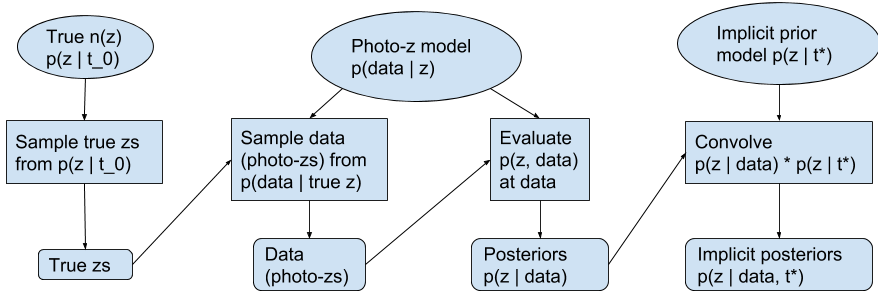
\includegraphics[width=\textwidth]{figures/chippr/flowchart.png}
		\caption{A flow chart illustrating the forward model used to generate mock data in the validation of \Chippr, as described in \Sect{sec:forward}.
		Ovals indicate a quantity I choose in order to generate the data, rectangles indicate an operation I perform, and rounded rectangles indicate a quantity created by the forward model.
		Arrows indicate the inputs and outputs of each operation performed to simulate mock \pzpdf\ catalogs.}
		\figlabel{fig:flowchart}
	\end{center}
\end{figure*}

The true redshift distribution used in these tests is a particular instance of the gamma function
\begin{equation}
\eqlabel{eqn:gamma}
n^{\dagger}(z) = \frac{1}{2 c_{z}} \left(\frac{z}{c_{z}}\right)^{2}\ \exp\left[-\frac{z}{c_{z}}\right]
\end{equation}
with $c_{z} = 0.3$, because it has been used in forecasting studies for \des\ and \lsst.
\aim{I learned this from talking to people and don't know of a published source that talks about the nitty gritty of the internal validation tests performed before there was data.}

The mock data emulates the three sources of error of highest concern to the \pz\ community: intrinsic scatter, catastrophic outliers, and systematic bias.
\Fig{fig:mega_scatter} illustrates these three effects individually at twice the tolerance of \lsst.
\begin{figure}
	\begin{center}
		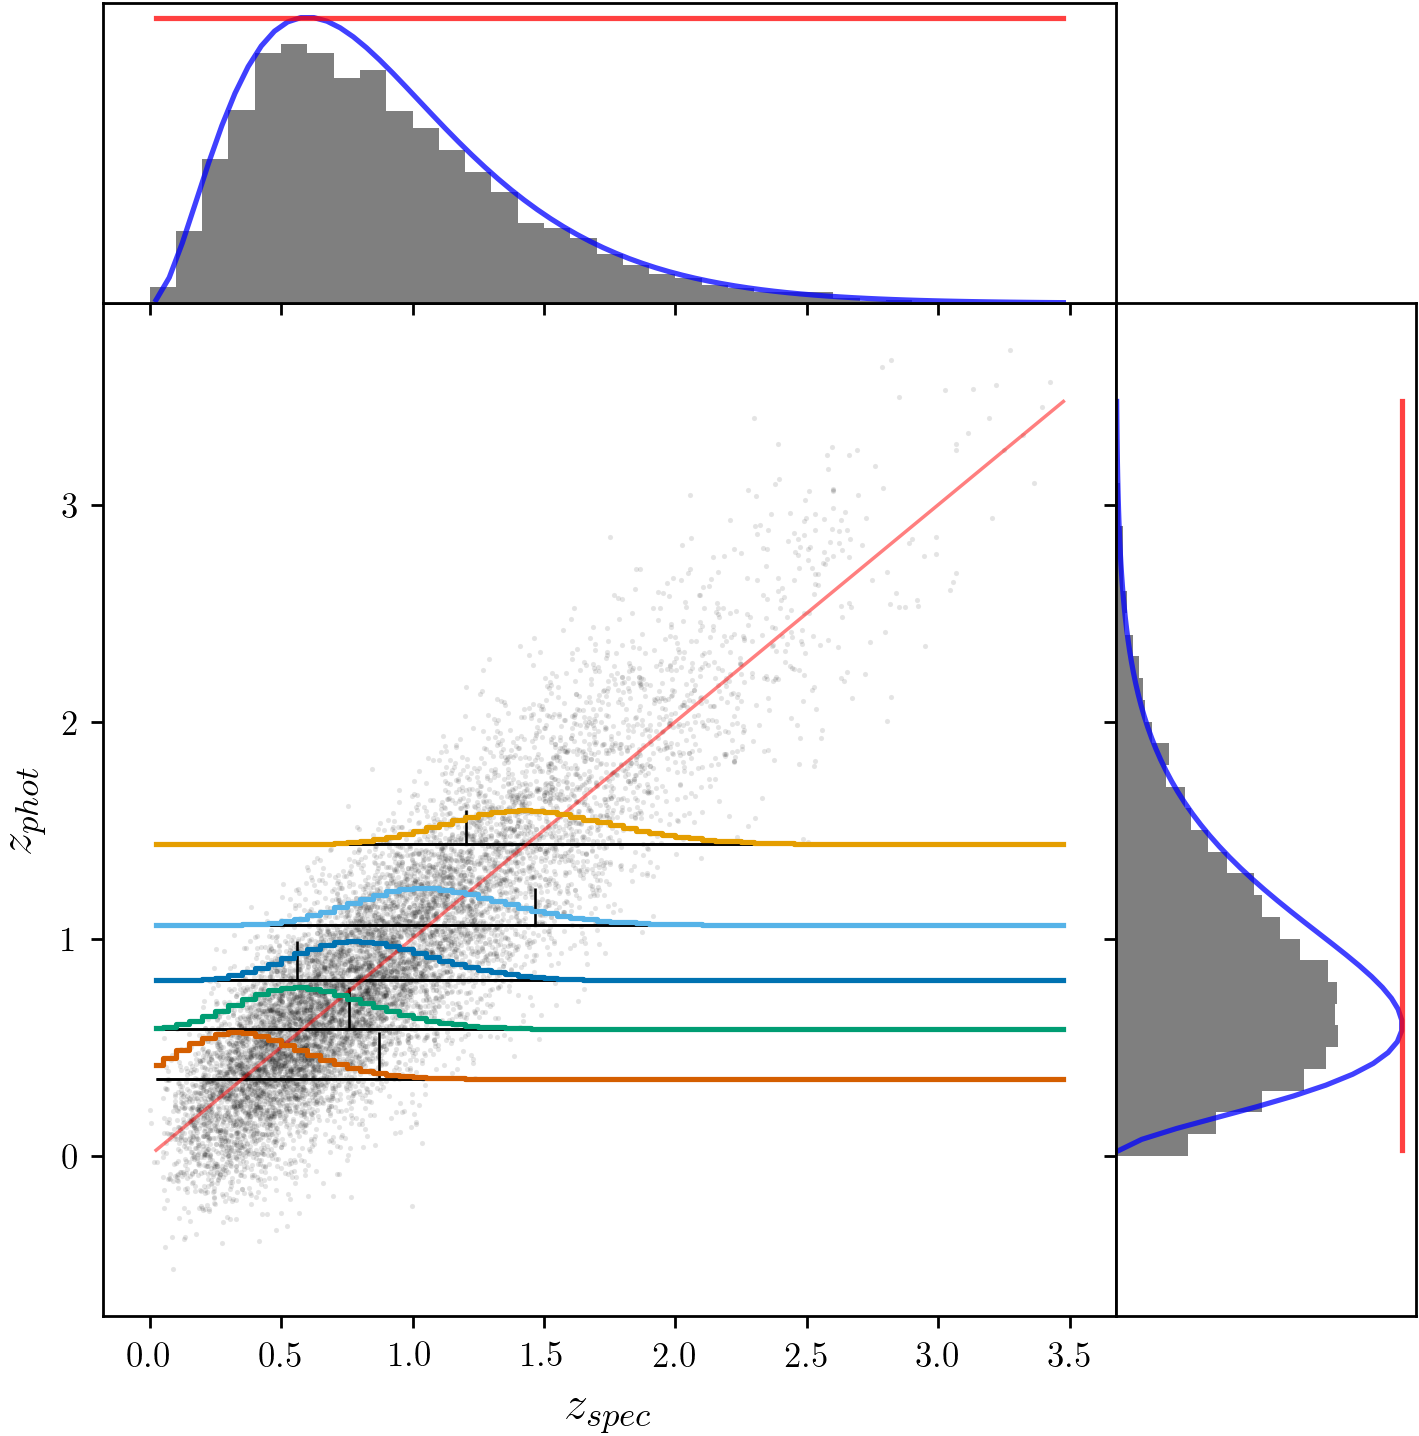
\includegraphics[width=0.3\textwidth]{figures/chippr/scatter_scatplot.png}
		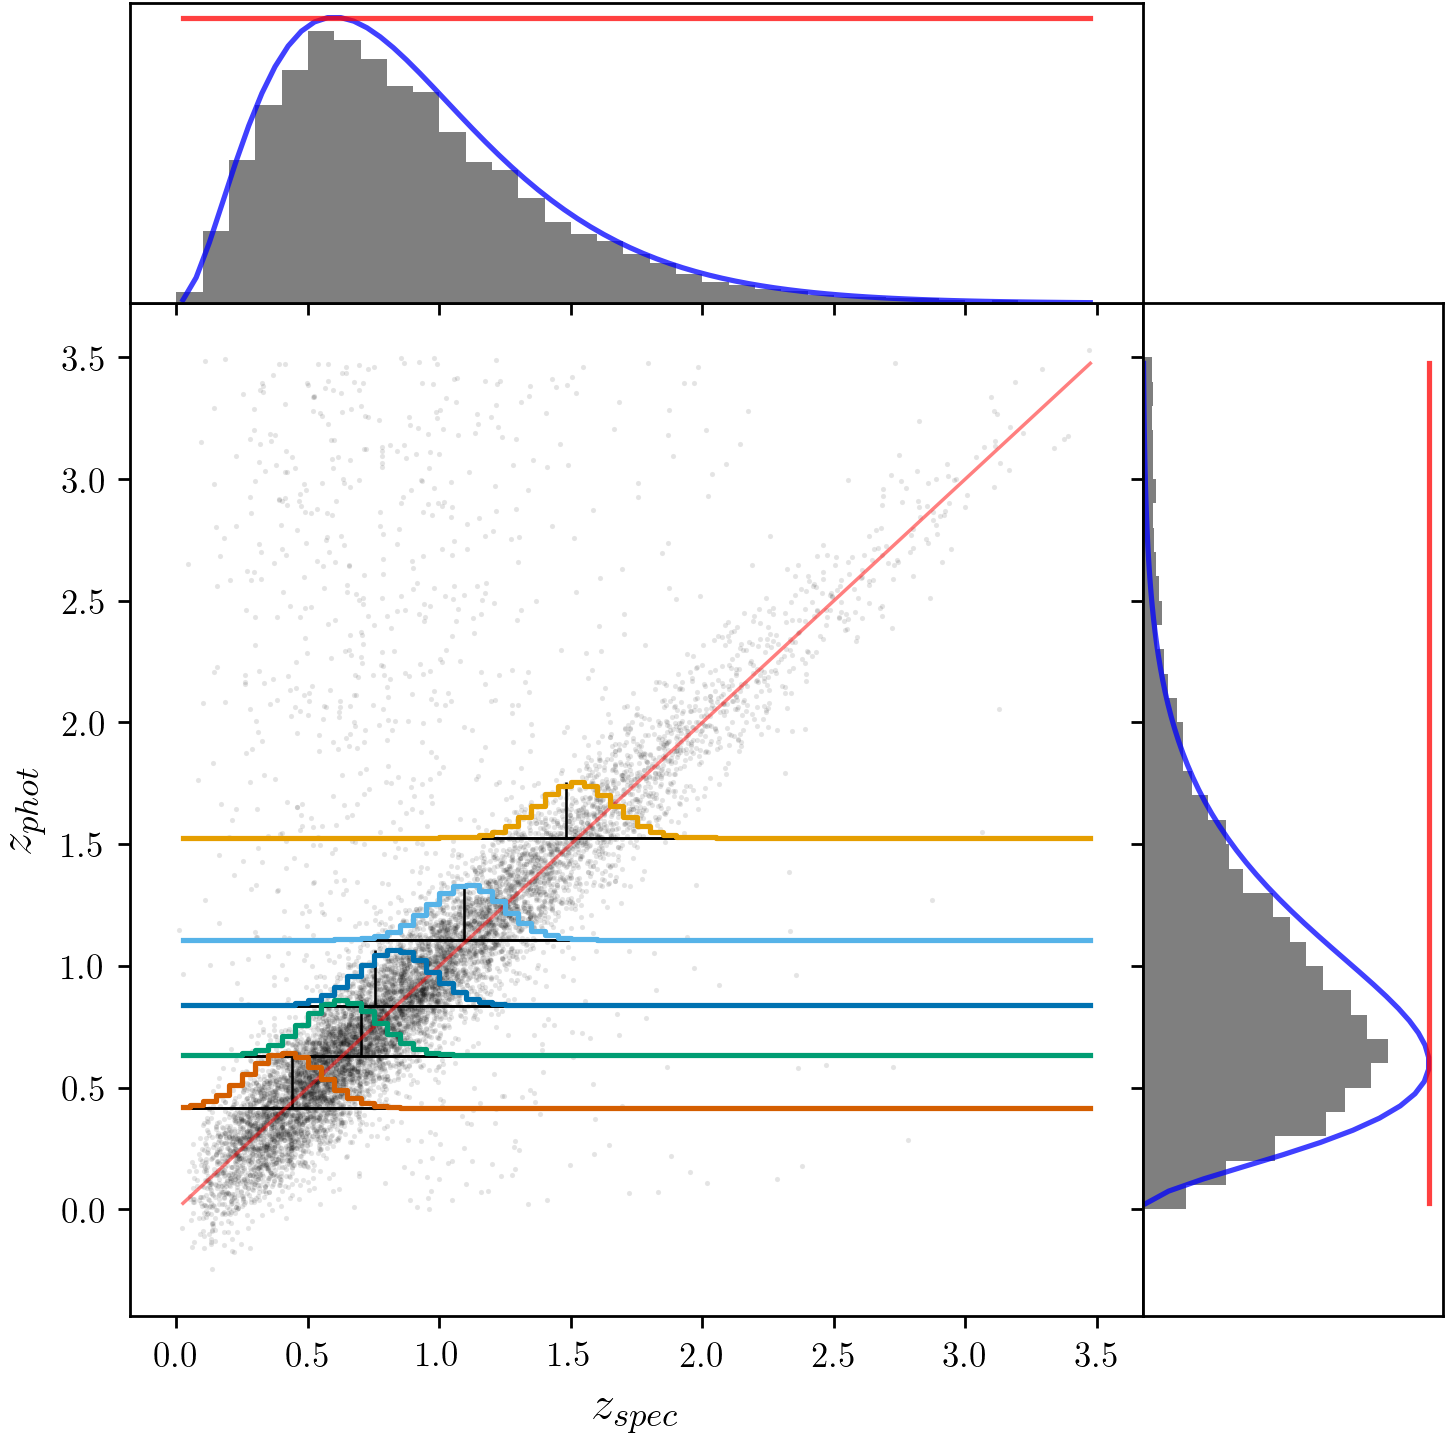
\includegraphics[width=0.3\textwidth]{figures/chippr/outlier_scatplot.png}
		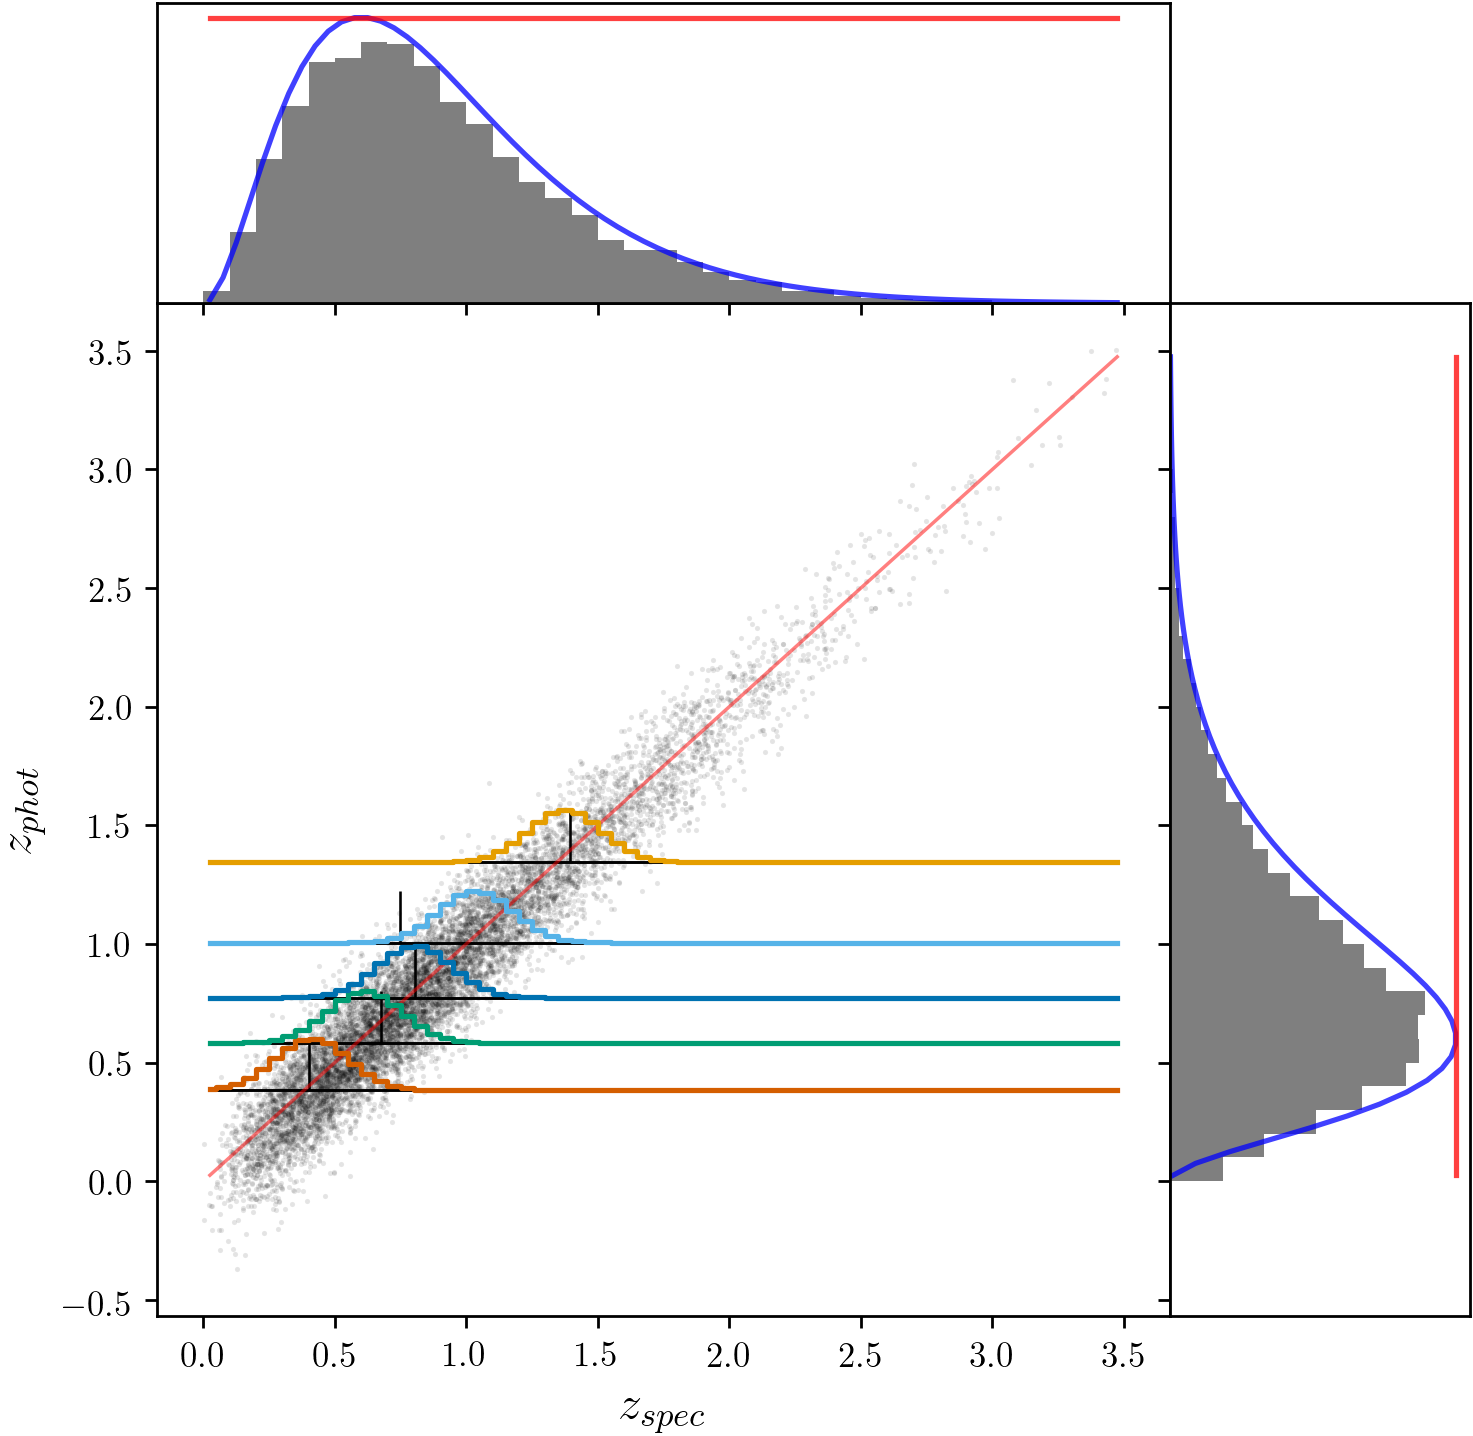
\includegraphics[width=0.3\textwidth]{figures/chippr/bias_scatplot.png}
		\caption{The joint probability space of true and estimated redshift for the three concerning \pz\ systematics: intrinsic scatter (left), uniform outliers (center), bias (right).
			The points indicate samples in the space of mock data and redshift, akin to the standard scatterplots of true and estimated redshift.
			Colored lines indicate posterior probabilities evaluated at the given estimated redshift.
			The insets show marginal histograms (gray) in each dimension, that can be compared with the true \nz\ used to make the figure (blue curve) to see the effect of the isolated systematic.
			\aim{Make the labels bigger if there's time for it.
			Also, fix the scaling on the insets.}
		}
		\figlabel{fig:mega_scatter}
	\end{center}
\end{figure}
Tests including all three effects at the tolerance levels of \lsst\ are presented in \Sect{sec:results}.
%In \Sect{sec:alldata} I describe the method by which mock \pzpdf s $\{\ln[\pr{z \gvn \data_{j}}]\}$ are synthesized as well as the real datasets considered for comparison.  

%The fiducial experiment of \Sect{sec:mock} is outlined first. 
%Seven other cases in \Sect{sec:imprecision} and \Sect{sec:inaccuracy} vary the \pzpdf s via the space of redshift and projected photometry.
%\Sect{sec:fake-data} considers unexpected true redshift density functions, and \Sect{sec:interim-data} considers nontrivial implicit priors.  
%Two additional cases with \sdss-III BOSS DR10 data are also considered in \Sect{sec:data}.
%The test cases included here are summarized in \Tab{tab:key}.
%
%\begin{table}
%	\begin{tabular}{llll}
%		\textul{Title} & \textul{True $n(z)$} & \textul{Implicit Prior} & 
%		\textul{Probability space}\\
%		Fiducial & Physically motivated, & Uniform & Single Gaussians\\
%		& featured $N(z)$ &&\\
%		Precise & Physically motivated, & Uniform & Single, Narrow Gaussians\\
%		& featured $N(z)$ &&\\
%		Imprecise & Physically motivated, & Uniform & Single, Broad Gaussians\\
%		& featured $N(z)$ &&\\
%		Trending & Physically motivated, & Uniform & Single Gaussians\\
%		& featured $N(z)$ && with $\sigma_{j}\sim z^{*}_{j}$\\
%		Multimodal & Physically motivated, & Uniform & Multiple Gaussians\\
%		& featured $N(z)$ &&\\
%		Sampled & Physically motivated, & Uniform & Sampled, Single Gaussian\\
%		& featured $N(z)$ &&\\
%		Featured & Single, Narrow Gaussian & Uniform & Single, Broad Gaussians\\
%		Unimodal $\vec{\theta}_{0}$ & Physically motivated, & Low-$z$ Favoring & 
%		Single, Broad Gaussians\\
%		& featured $N(z)$ &&\\
%		Bimodal $\vec{\theta}_{0}$& Physically motivated, & Mid-$z$ Disfavoring & 
%		Single, Broad Gaussians\\
%		& featured $N(z)$ &&\\
%		Surveyed & Unknown & \citet{Sheldon2012} & pseudo-random sample of BOSS DR10\\
%		Biased & Unknown & \citet{Sheldon2012} & brightest 50\% of BOSS test
%	\end{tabular}
%	\caption{Summary of the mock data validation tests using the shorthand names by which the tests are referenced.}
%	\tablabel{tab:key}
%\end{table}

The hyperprior distribution chosen here is a multivariate normal distribution with mean $\vec{\mu}$ equal to the implicit prior $\ndphi^{*}$ and covariance
\begin{equation}
\eqlabel{eqn:priorcov}
\Sigma_{k,k'} = q\ \exp[-\frac{e}{2}\ (\bar{z}_{k}-\bar{z}_{k'})^{2}]\ +\ t\delta(k,k')
\end{equation}
inspired by one used in Gaussian processes, where $k$ and $k'$ are indices ranging from $1$ to $K$ and $q=1.0$, $e=100.0$, and $t=q\cdot10^{-5}$ are constants chosen to permit draws from this prior distribution to produce shapes similar to that of a true $\tilde{\ndphi}$.  
We adapt the full log-posterior of \Eq{eqn:final} to the chosen binning of redshift space.
An example of such samples from the prior are shown in \Fig{fig:prior}.

\begin{figure}
%	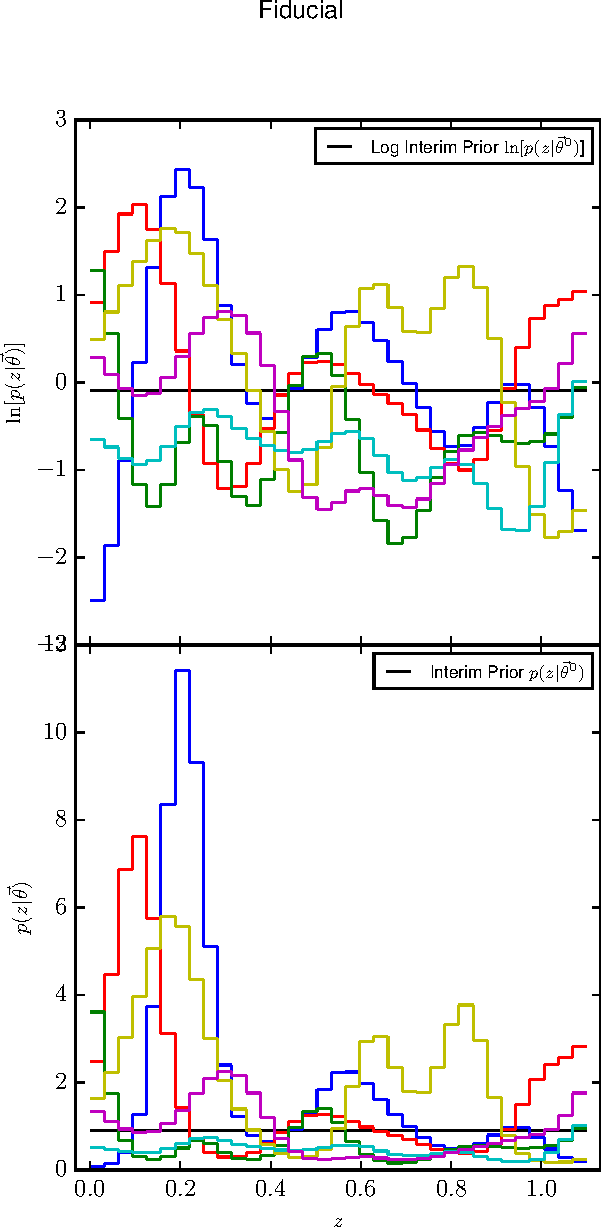
\includegraphics[width=0.5\textwidth]{figures/chippr/null_priorsamps.pdf}
	\caption{\aim{I need to remake this one because it uses the wrong notation and I stopped making it automatically a while ago.}
		Samples (colored lines) of $\pr{z \gvn \ndphi}$ where each $\ndphi$ is drawn from the hyperprior distribution $\pr{\ndphi}$ given in \Eq{eqn:priorcov}.}
	\figlabel{fig:prior}
\end{figure}

The sampler is initialized with $W=100$ walkers each with a value chosen from a Gaussian distribution of identity covariance around a sample from the hyperprior distribution.  

%\Sect{sec:fake-data} considers a delta function true redshift distribution, but the other sections consider only this physically motivated true \nz.
%\aim{Discuss why it perhaps shouldn't be considered physically motivated -- might not have decided that's what the real thing looks like if we hadn't been stacking all along}

%\subsection{Toy Model}
%\sectlabel{sec:fake-data}
%
%\aim{Commented out but may add back in later.}

%We test the sampler in a case of a highly unrealistic but strongly featured true $N(z)$, that of the lower panel of \Fig{fig:physpz}.  
%This is done to show that the sampler works even in extreme and unanticipated conditions.  
%Instead of sampling the physically motivated true distribution $p(z|\vec{\theta}')$ as in \Sect{sec:mock}, we as

%\Fig{fig:toy-comp} compares the mean of the posterior samples to the results of stacking and marginalized likelihood maximization.  
%It can be seen that the marginalized maximum likelihood estimator is best at recovering the true distribution approaching a delta function due to the nature of the optimizer, which considers each component of the hyperparameter vector to be independent of all others.  
%Other estimators predict a broader distribution than the truth, with stacking broadening it the most and the mean of the samples broadening it the least.  
%Though the sampler does not consider components of the hyperparameter vector to be independent, it is flexible enough to provide good constraints on the true $N(z)$.
%
%\begin{figure}
%	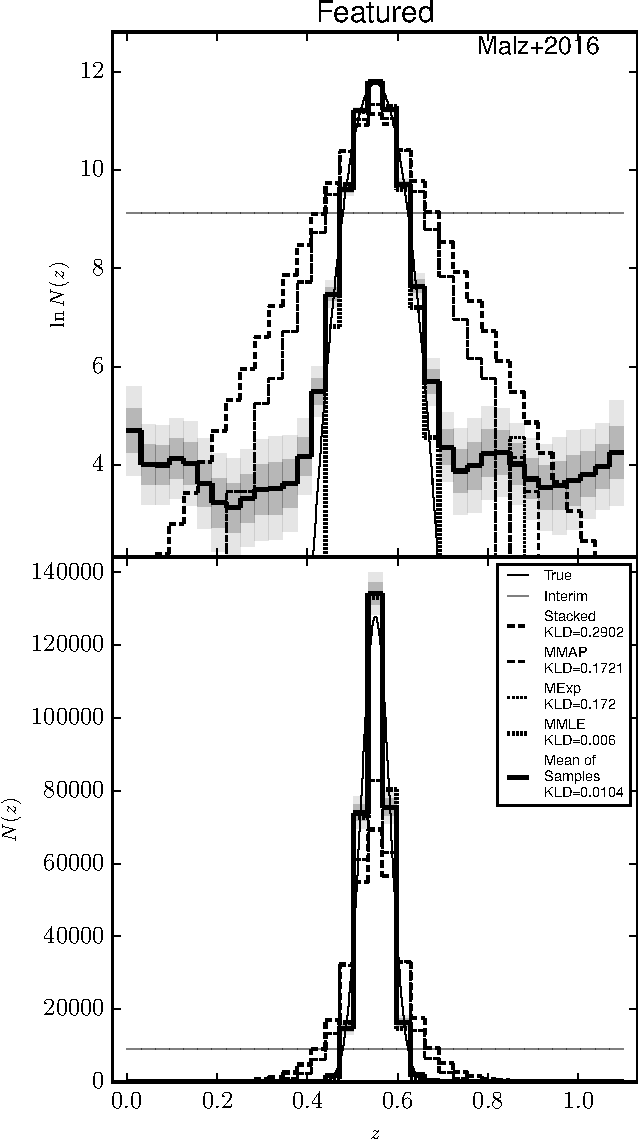
\includegraphics[width=0.5\textwidth]{figures/chippr/delt_comps.pdf}
%	\caption{In this case, the marginalized maximum likelihood estimator (thick, dotted line) recovers the true $N(z)$ (thin, solid line) better than the mean of posterior samples (thick, solid line), though the error bars ($1\sigma$ in dark gray, $2\sigma$ in light gray) do include the true values of the hyperparameters. 
%		The stacked estimator (thick, dashed line) is the worst estimator of the true redshift distribution function, while the marginalized maximum a posteriori estimator (thin, dashed line) and marginalized expected value estimator (thin, dotted line) are not quite as broad.}
%	\figlabel{fig:toy-comp}
%\end{figure}

\subsection{Intrinsic Scatter}
\sectlabel{sec:scatter}

\Fig{fig:pzs-scatter} shows some examples of \pzpdf s generated with only the systematic of intrinsic scatter.
One can see that the histogram of redshift estimates is broader than that of true redshifts, and that the effect is substantially more pronounced by just doubling the intrinsic scatter from the level of the \lsst\ requirements.

\begin{figure}
	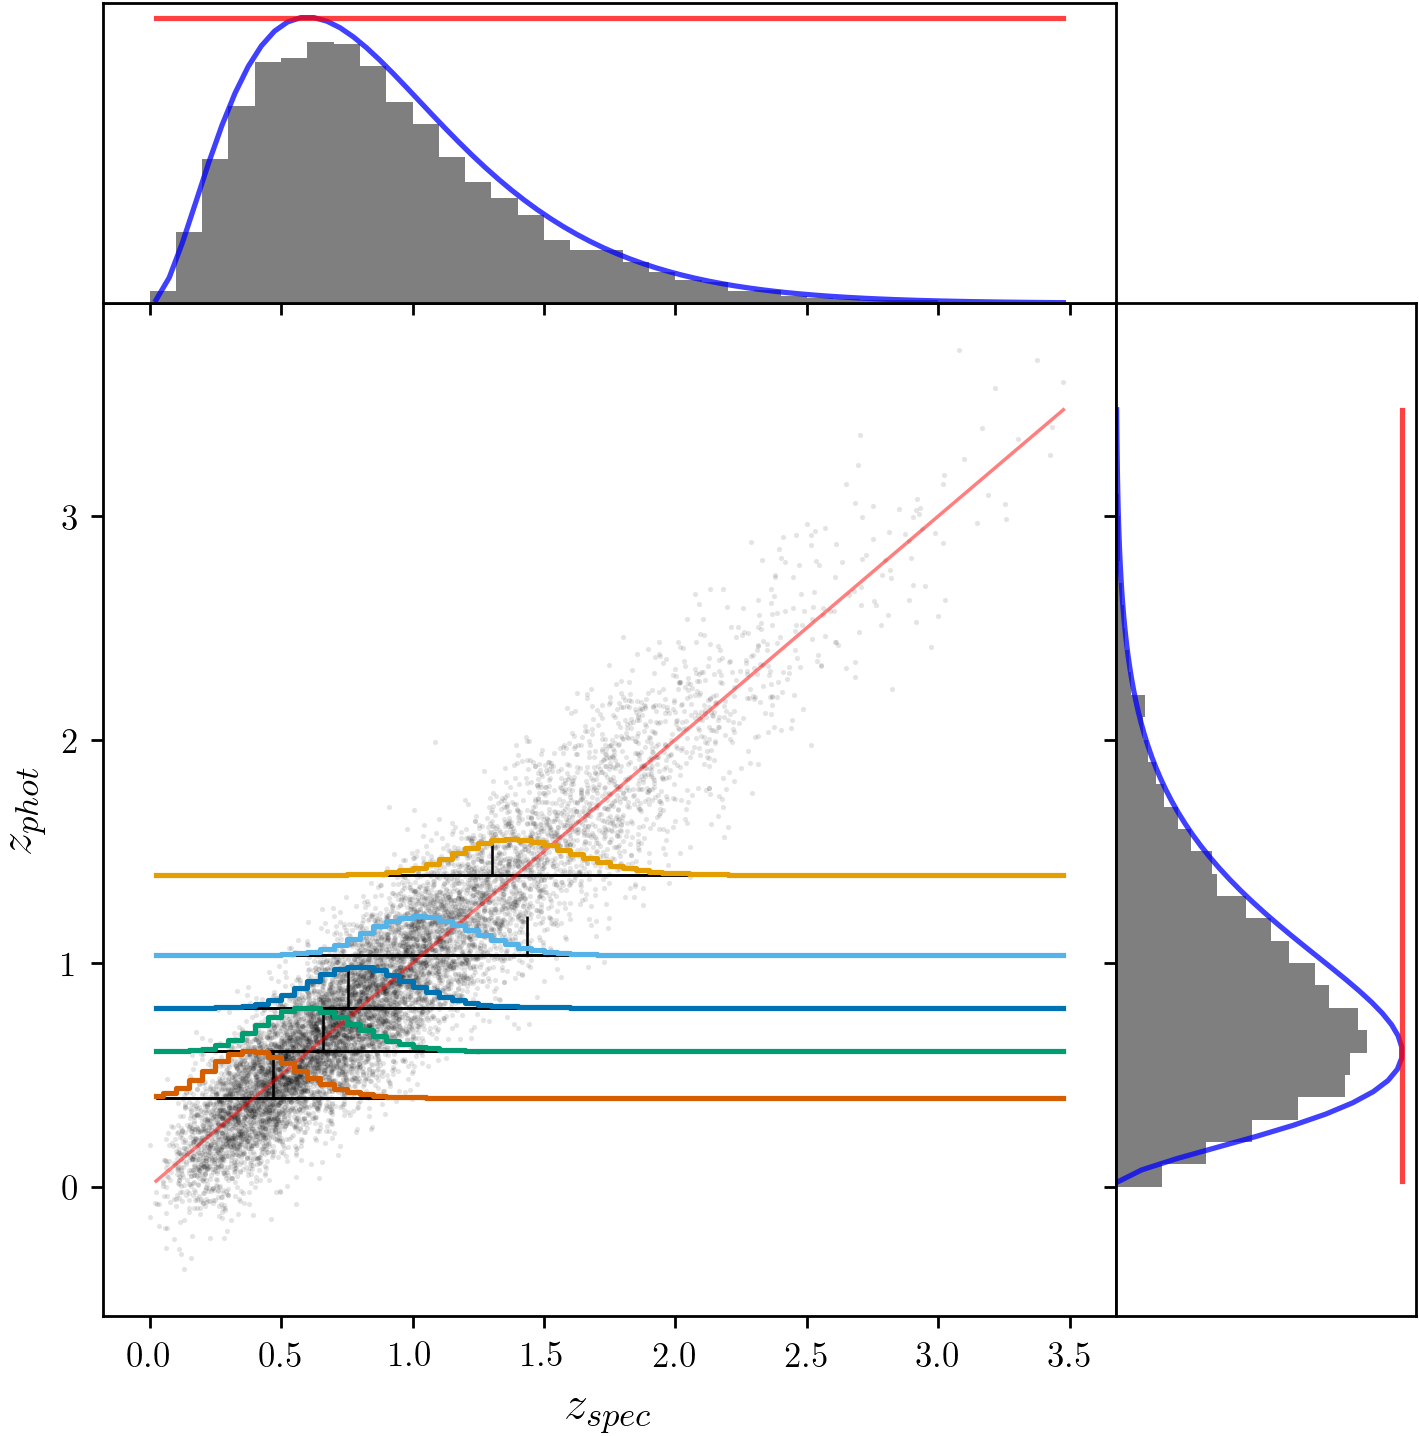
\includegraphics[width=0.5\textwidth]{figures/chippr/samplepzs_scatter1.png}
	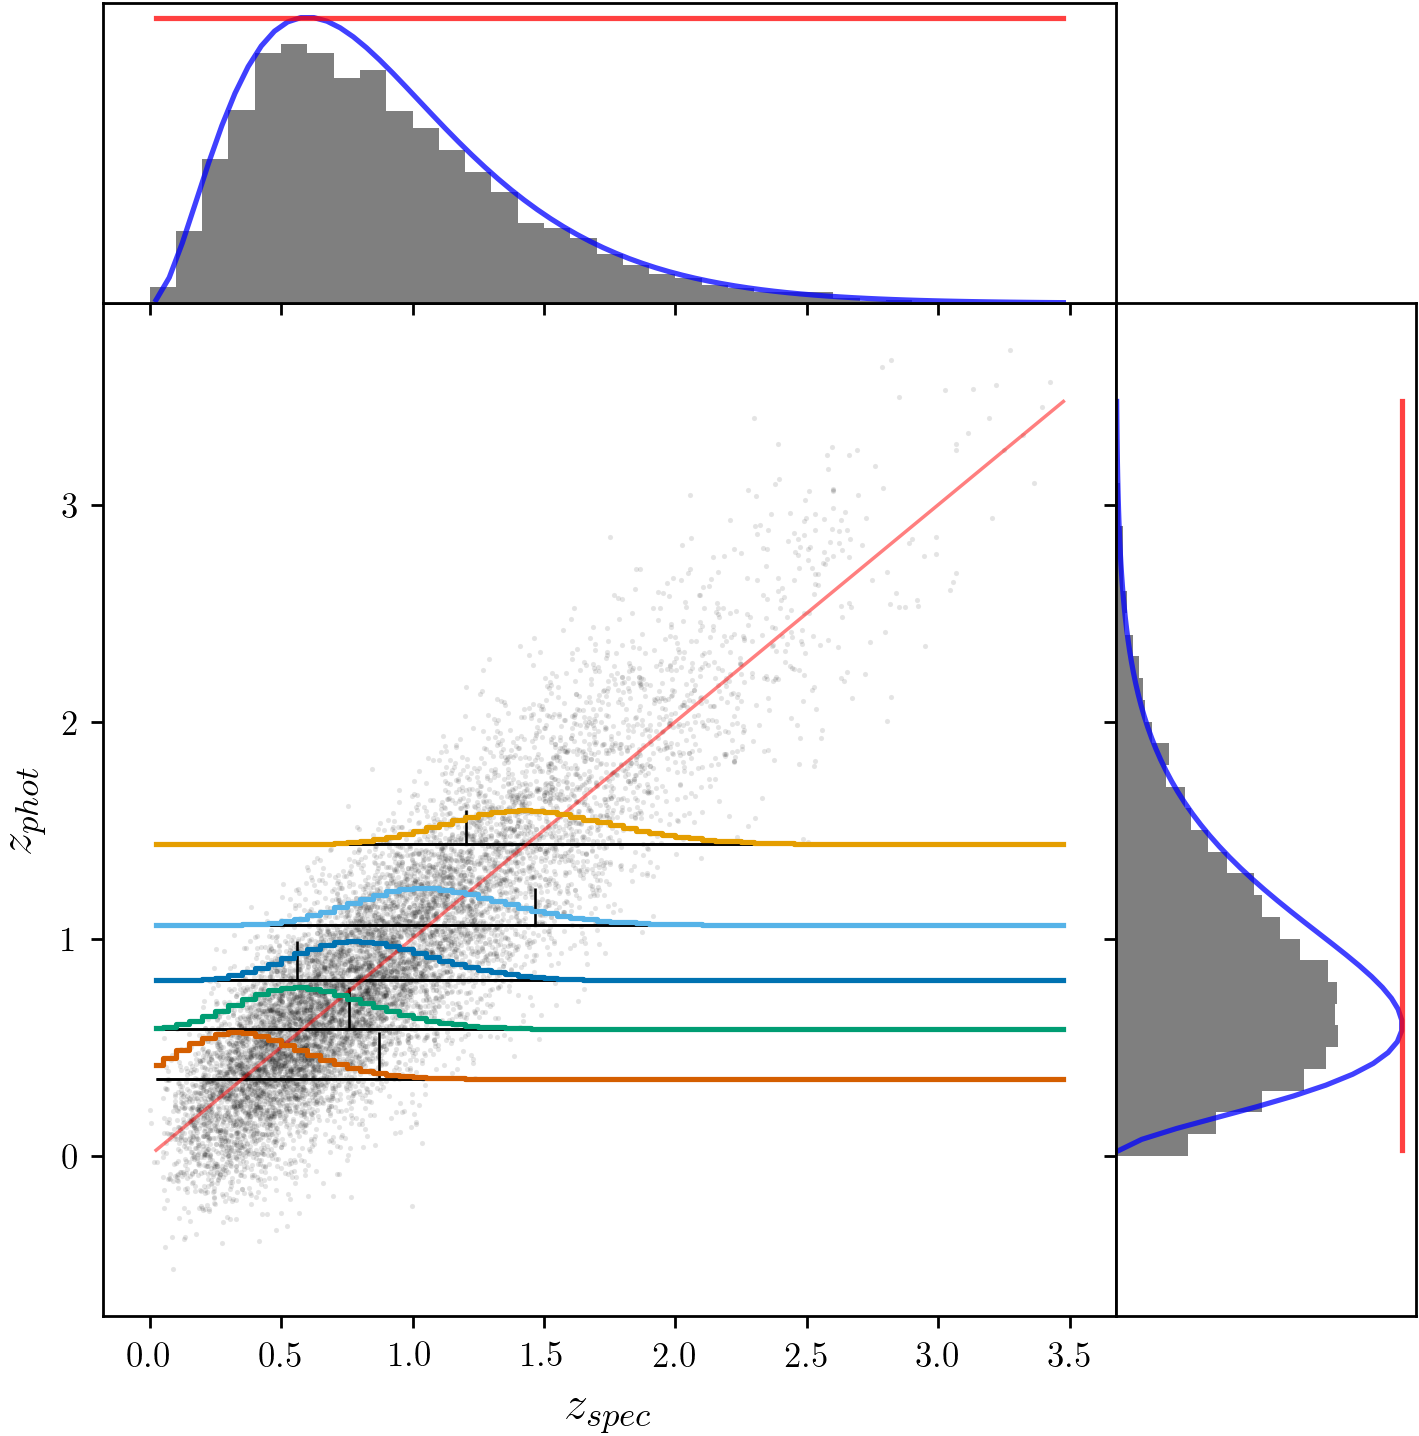
\includegraphics[width=0.5\textwidth]{figures/chippr/samplepzs_scatter2.png}
	\caption{
		Examples of mock \pzpdf s (colored lines) generated with intrinsic scatter at the \lsst\ requirements (left) and twice the \lsst\ requirements (right), including samples from the probability space of true and observed redshift (black points), \pzpdf s (colored lines), the true redshifts of the example \pzpdf s (black vertical lines).
		A histogram (gray) of points in each dimension is shown in the respective inset, with the true redshift distribution (blue curve) and implicit prior (red curve).
	}
	\figlabel{fig:pzs-scatter}
\end{figure}

\Fig{fig:results-scatter} shows the results of \Chippr\ and the alternative approaches.
As expected, the estimates of \nz\ based on the modes of the \pzpdf s and stacking are broader than the marginalized maximum likelihood estimator from \chippr.
Though the marginalized maximum likelihood estimator is unaffected, the \Chippr\ posterior distribution on the redshift distribution is itself broader for the higher intrinsic scatter case than for the \lsst\ requirements.
A broader posterior on \nz\ is an expected consequence of any increase in uncertainty of the \pzpdf s, but the invariance of the marginalized maximum likelihood estimator .

\begin{figure}
	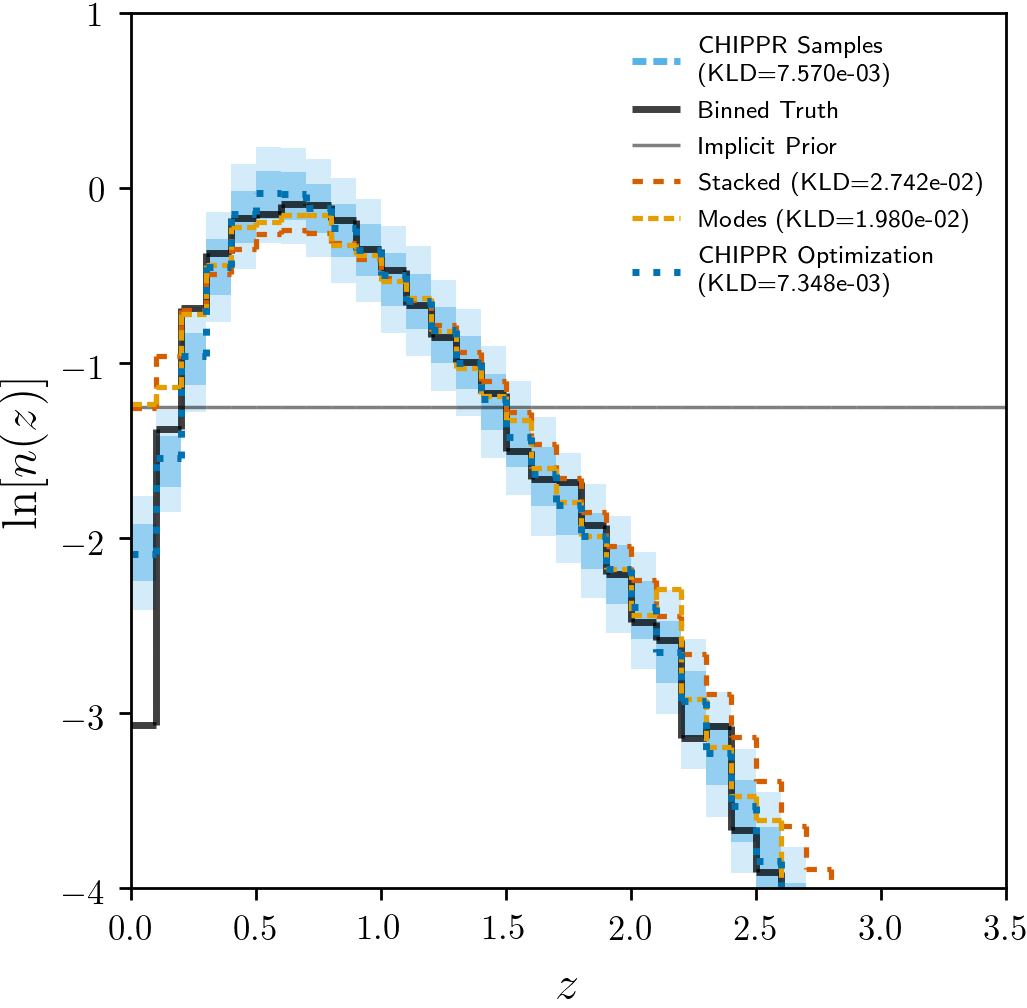
\includegraphics[width=0.5\textwidth]{figures/chippr/results_scatter1.png}
	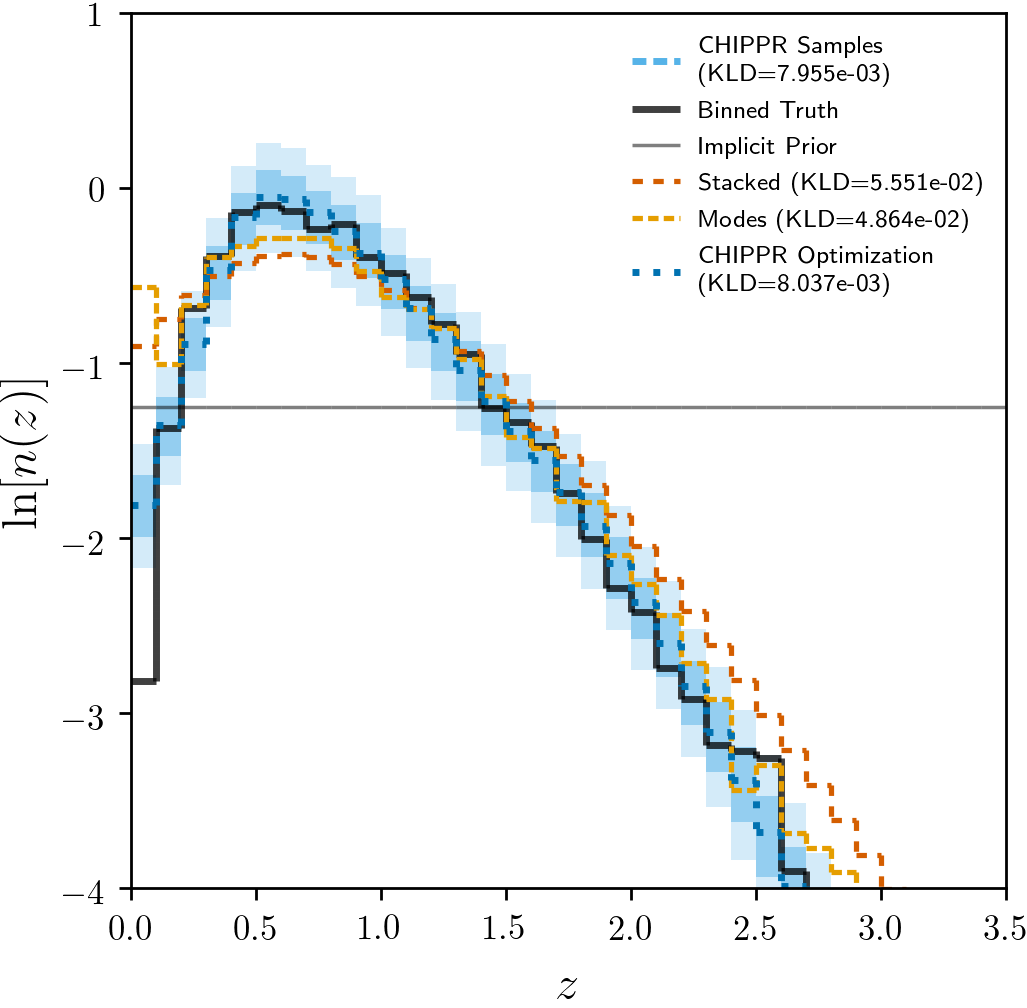
\includegraphics[width=0.5\textwidth]{figures/chippr/results_scatter2.png}
	\caption{
		The results of \Chippr\ (samples in light blue and optimization in dark blue) and the alternative approaches (the stacked estimator in red and the histogram of modes in yellow) on \pzpdf s with intrinsic scatter of the \lsst\ requirements (left) and twice that (right), with the true redshift density (black curve) and implicit prior (gray curve).
		\Chippr\ is robust to intrinsic scatter, but the alternatives suffer from overly broad \nz\ estimates that worsen with increasing intrinsic scatter.
	}
	\figlabel{fig:results-scatter}
\end{figure}

\subsection{Catastrophic Outliers}
\sectlabel{sec:outliers}

As was covered in the Introduction \aim{add an internal reference}, catastrophic outliers tend to be distributed non-uniformly across the space of observed and true redshift.
However, the \lsst\ requirements do not specify details for a distribution of outliers to which they were tuned, and it is still instructive to examine the impact of uniform outliers on the inference of \nz.
More realistic outlier populations will be covered in \Sect{sec:results}.

A uniformly distributed population of outliers was simulated by giving every sample in true redshift a $10\%$ chance of having an observed redshift drawn from a uniform distribution rather than the Gaussian about the true redshift.
Though this results in slightly less than the $10\%$ catastrophic outlier rate, it can be done independently of the definition of the standard deviation so was implemented for demonstrative purposes.
\Fig{fig:uniform-outliers} shows examples of \pzpdf s from a uniformly distributed outlier population at the level of the \lsst\ requirements as well as the results of \Chippr\ and other \nz\ estimation methods.
The alternative estimators are overly broad, whereas \Chippr\ yields an unbiased estimate of \nz.

\begin{figure}
	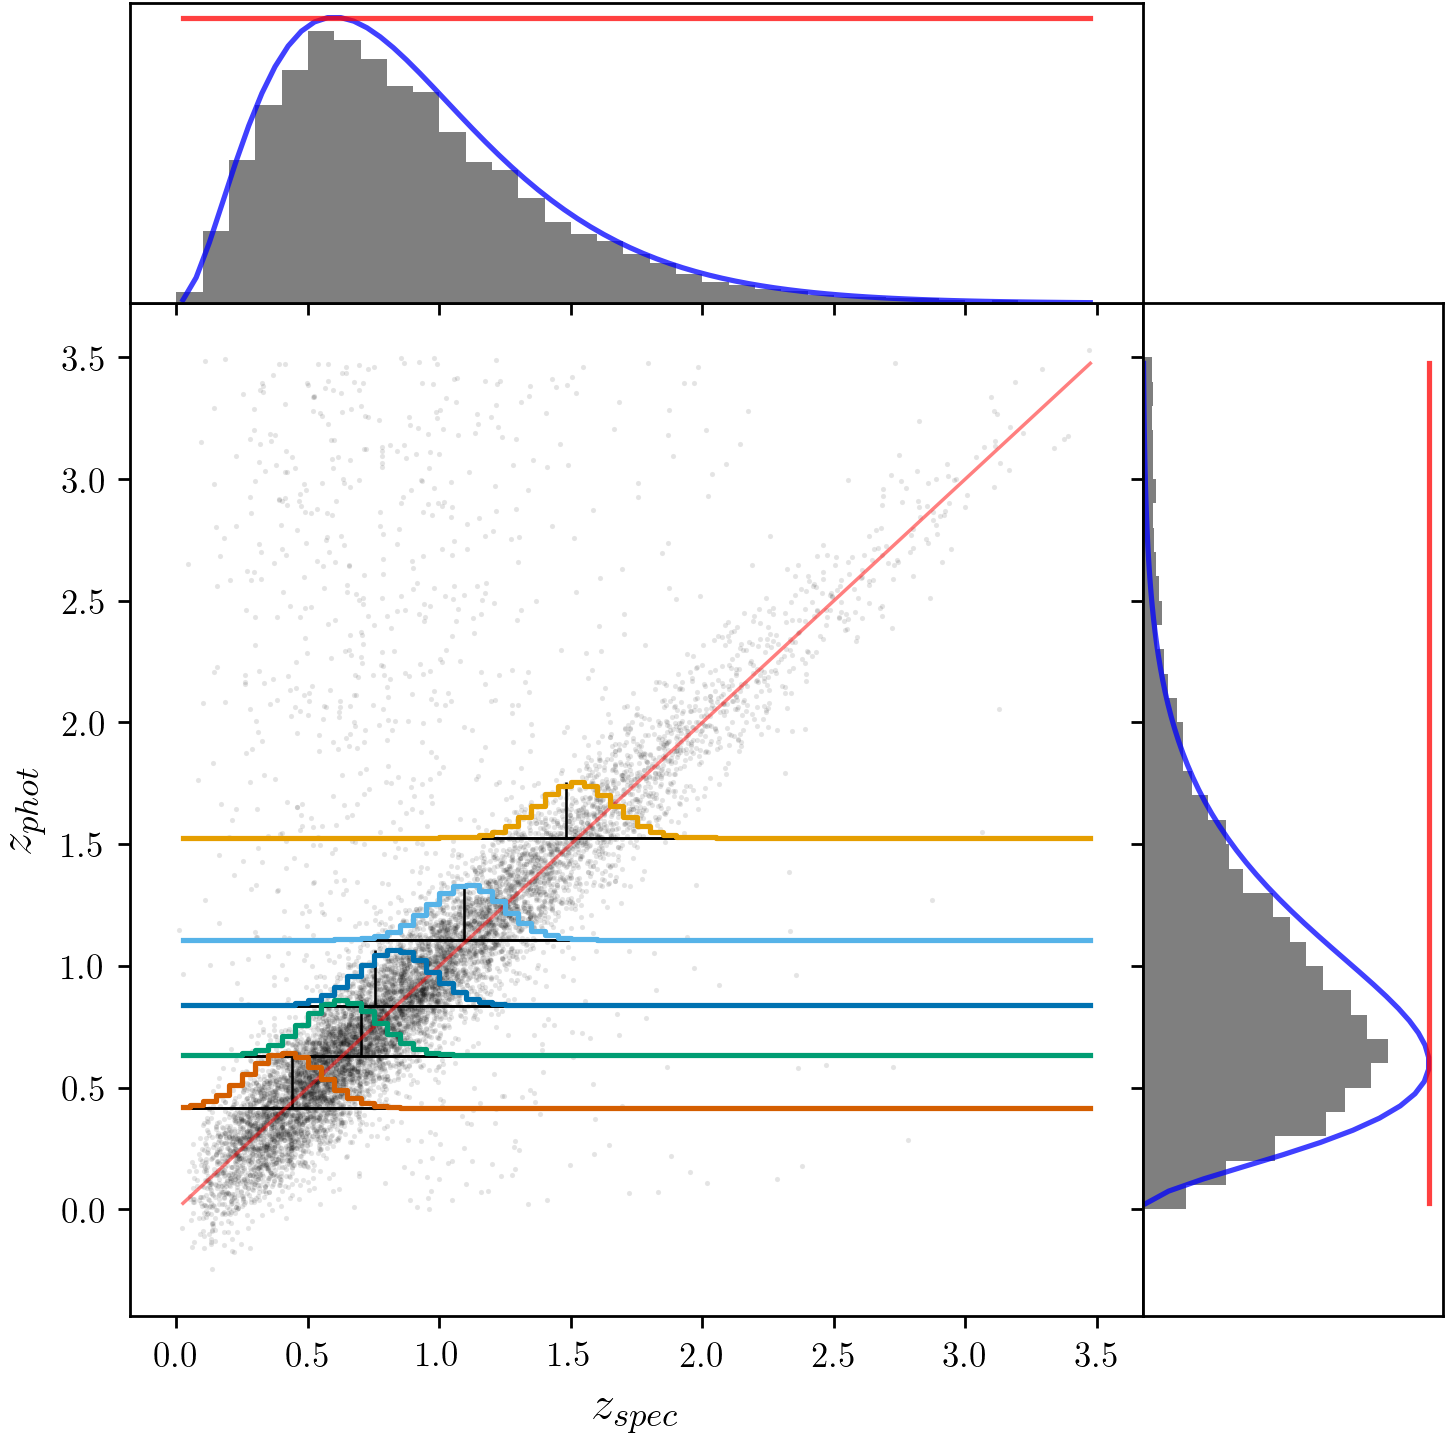
\includegraphics[width=0.5\textwidth]{figures/chippr/single_uout_mega_scatter.png}
	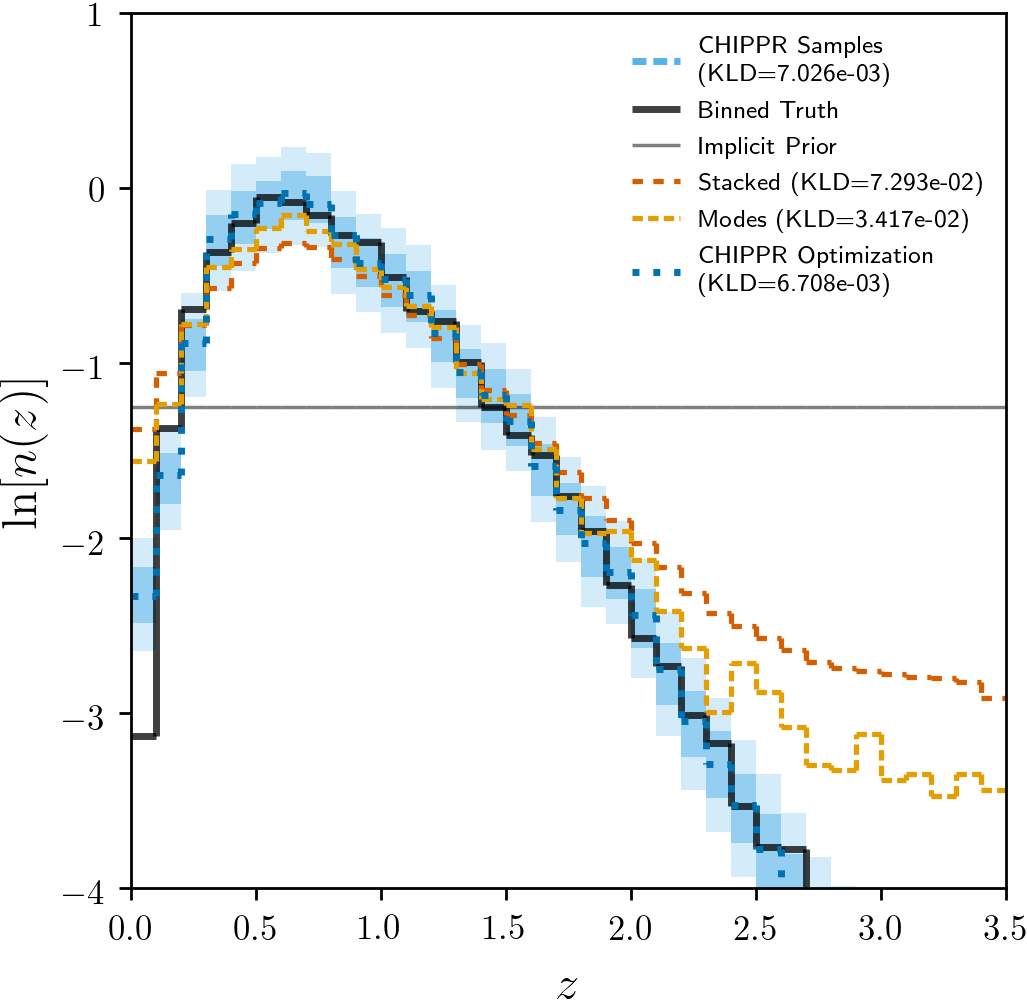
\includegraphics[width=0.5\textwidth]{figures/chippr/single_uout_log_estimators.png}
	\caption{
		Left: Examples of \pzpdf s with a uniform catastrophic outlier population at the level of the \lsst\ requirements, including samples from the probability space of true and observed redshift (black points), \pzpdf s (colored curves), and the true redshifts of the example \pzpdf s (black vertical lines), with marginal histograms (gray) for each dimension with the true redshift distribution (blue curve) and implicit prior (red curve) in the insets.
		Right: The results of \Chippr\ (samples in light blue, optimization in dark blue) and the alternative approaches (the stacked estimator in red, the histogram of modes in yellow) on \pzpdf s with uniformly distributed catastrophic outliers, with the true redshift density (black curve) and implicit prior (gray curve).
		The presence of the catastrophic outlier population broadens the histogram of modes and stacked estimator of the redshift distribution, but the result of \Chippr\ is unbiased.
	}
	\figlabel{fig:uniform-outliers}
\end{figure}

When one thinks of the \pzpdf s of catastrophic outliers, however, what comes to mind is multimodal \pzpdf s, wherein reducing \pzpdf s to point estimates to make a standard scatterplot of the true and observed redshifts leads to substantial probability density off the diagonal.
These coordinated catastrophic outliers may be emulated in the joint probability space of true and estimated redshifts by using a mixture of the unbiased diagonal defined by the intrinsic scatter and an additional Gaussian in one dimension, with constant observed redshift for a template-fitting code and constant true redshift for a machine learning code.
In the case of a catastrophic outlier population like that anticipated of template-fitting codes, $10\%$ of all galaxies have their observed redshift at a particular value unrelated to their true redshift, illustrated in the left panel of \Fig{fig:nonuniform-outliers-data}.
This case is subject to the same caveat as the uniformly distributed outliers when it comes to the \lsst\ requirement.

It is less straightforward to emulate catastrophic outliers like those anticipated of a machine learning code.
The test here gives $10\%$ of galaxies at the redshift affected by outliers an observed redshift that is uniformly distributed relative to the true redshift, illustrated in the right panel of \Fig{fig:nonuniform-outliers-data}.
This means that far fewer than $10\%$ of all galaxies in the sample are catastrophic outliers.
\aim{Probably won't have time to change code to address this inconsistency}
This second variety of outliers is the only kind that can lead to multimodal \pzpdf s under the forward model.
\aim{Interpret this in terms of whether BPZ, etc. are yielding likelihoods and how it relates to the standard true vs. estimated redshift plot presented in the introduction.}

\begin{figure}
	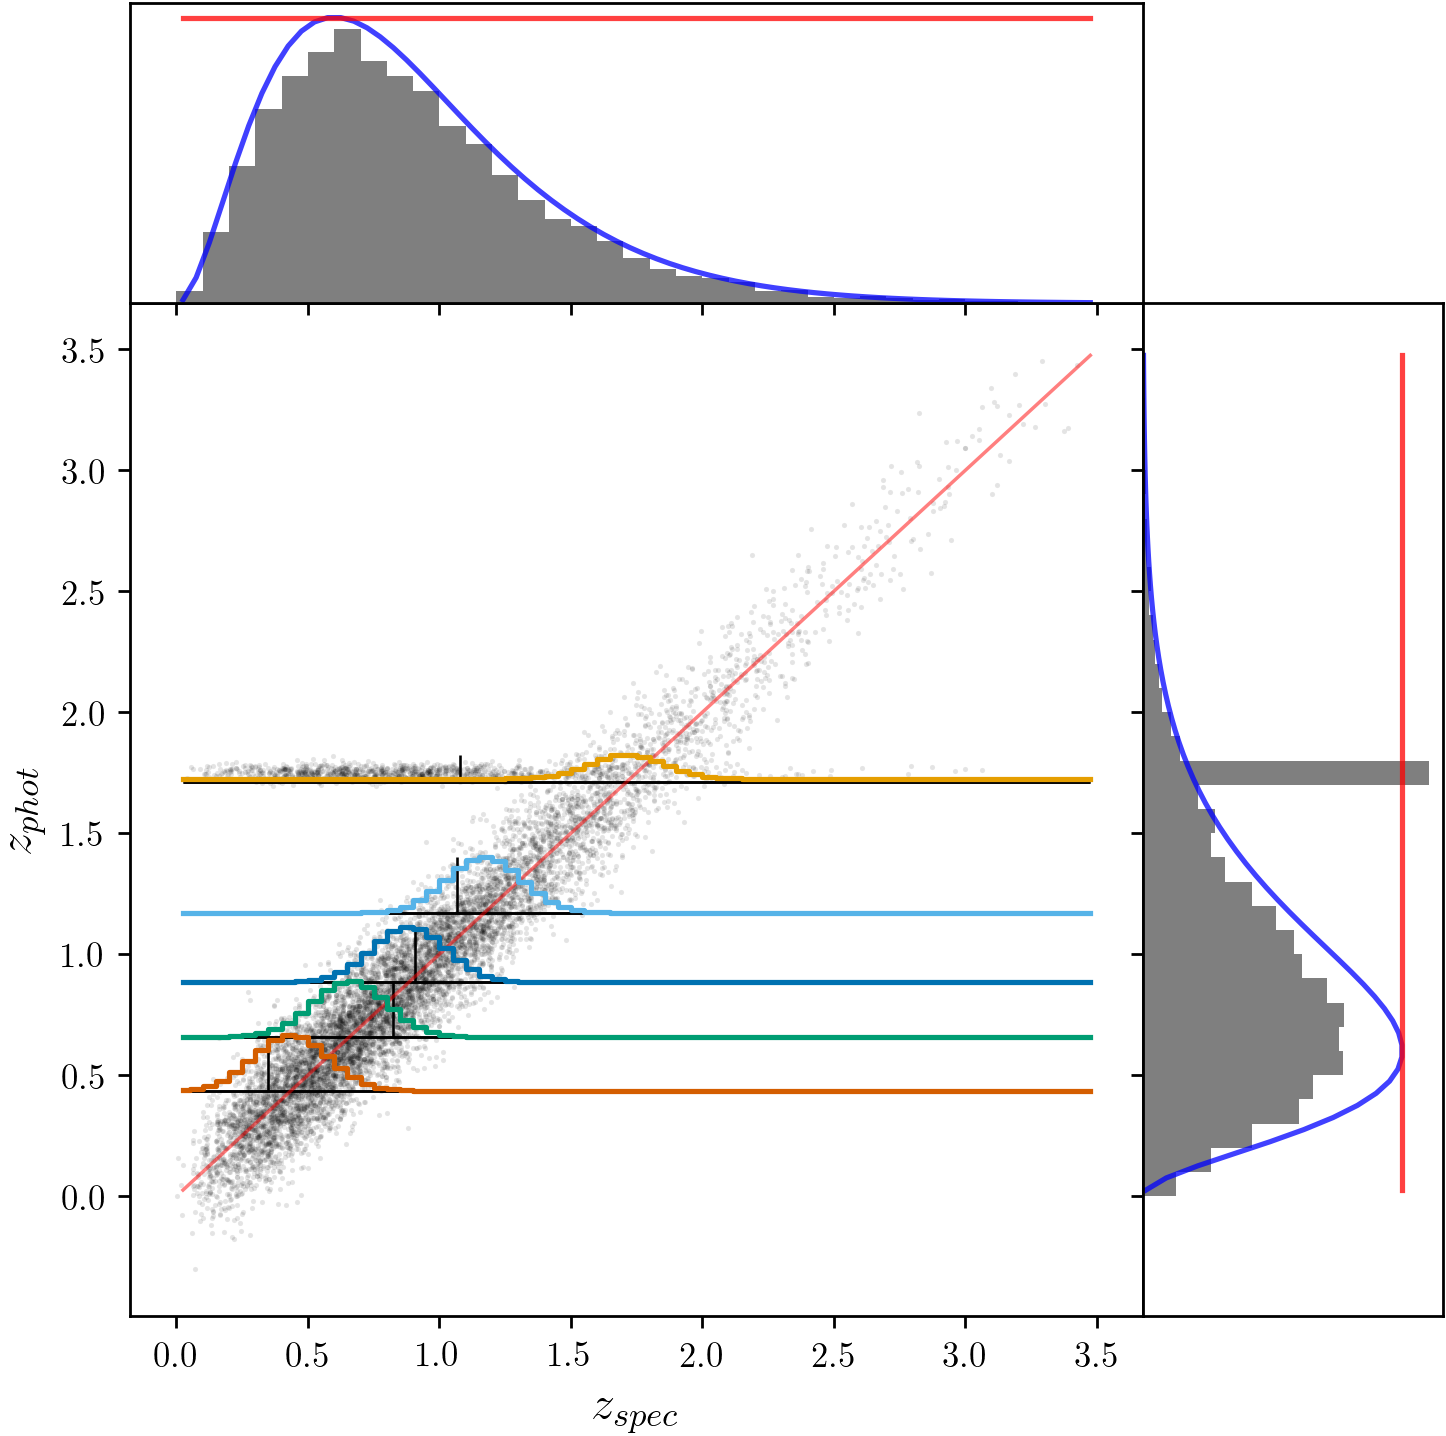
\includegraphics[width=0.5\textwidth]{figures/chippr/thesis_eout_mega_scatter.png}
	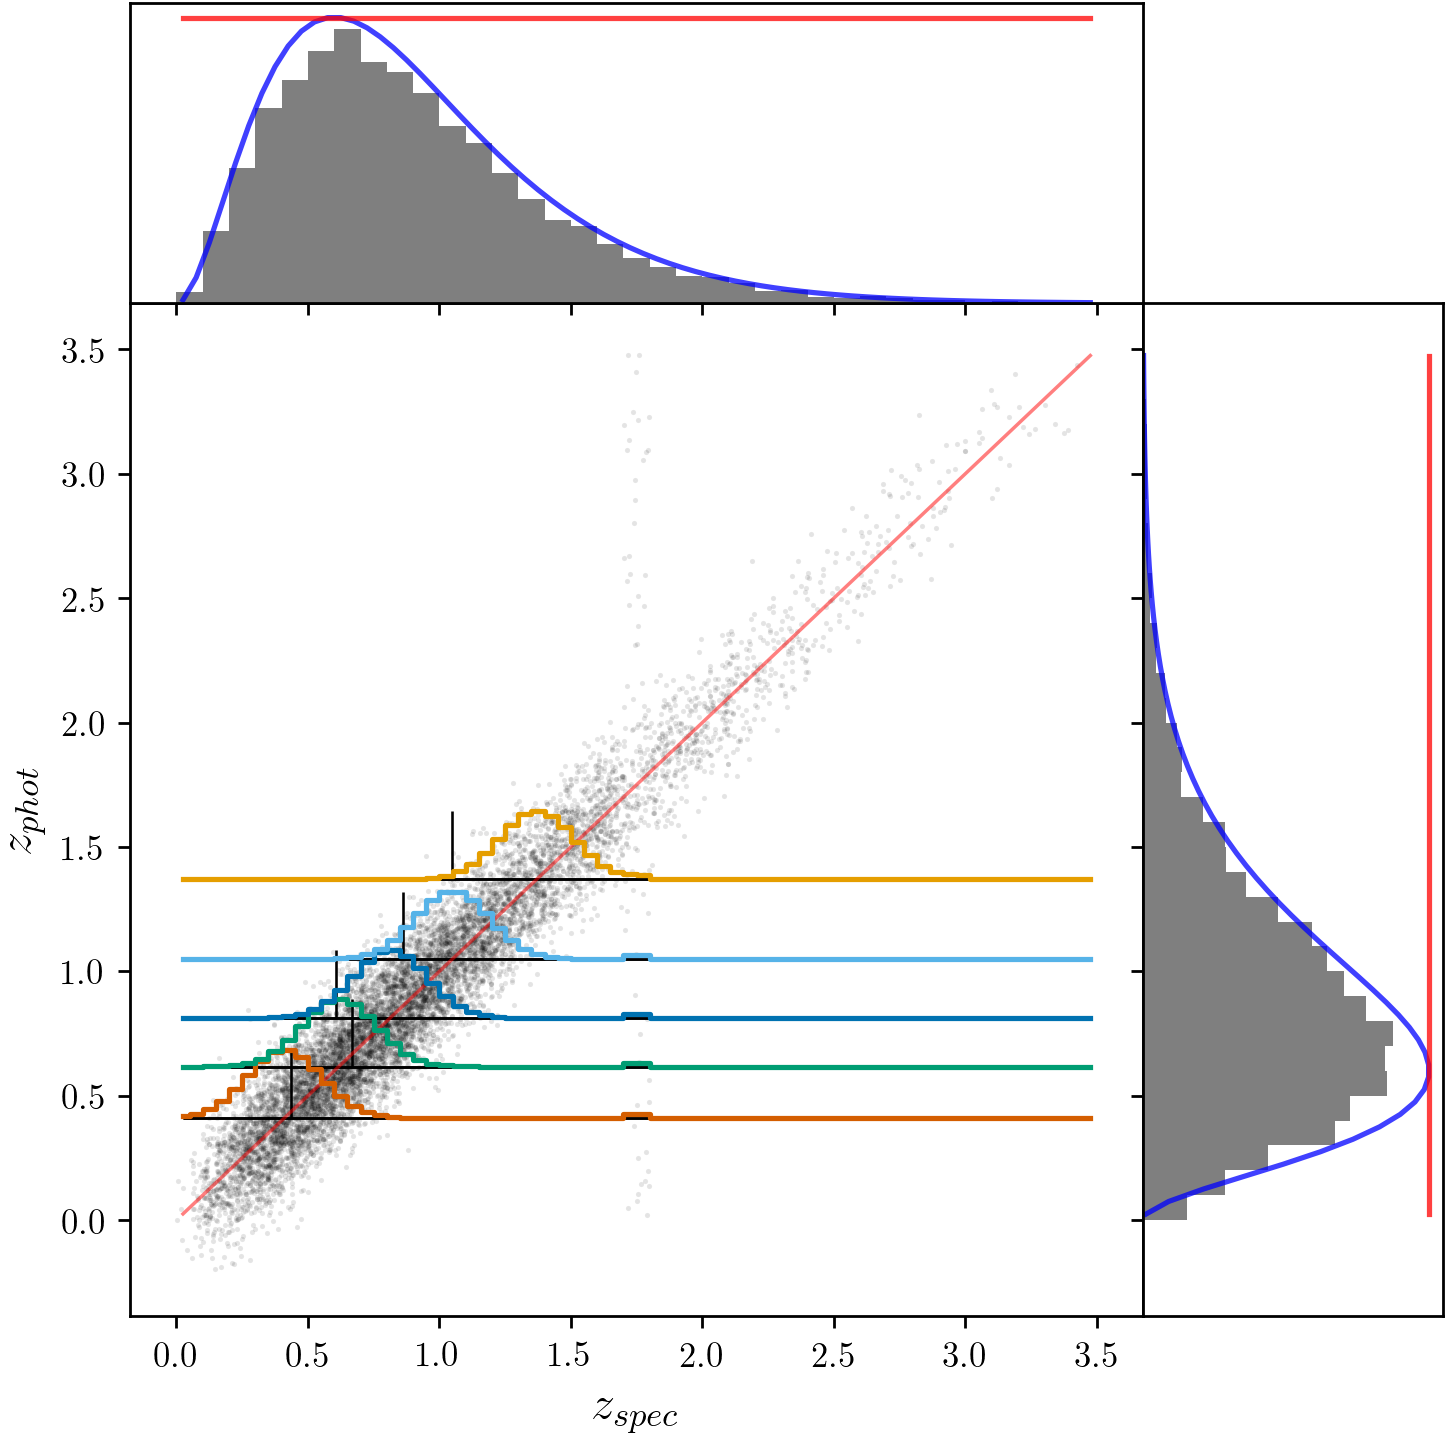
\includegraphics[width=0.5\textwidth]{figures/chippr/thesis_rout_mega_scatter.png}
	\caption{
		Examples of \pzpdf s with a catastrophic outlier population like that seen in template-fitting \pzpdf\ codes (left) and machine learning \pzpdf\ codes (right), including samples from the probability space of true and observed redshift (black points), \pzpdf s (colored curves), and the true redshifts of the example \pzpdf s (black vertical lines), with marginal histograms (gray) for each dimension with the true redshift distribution (blue curve) and implicit prior (red curve) in the insets.
	}
	\figlabel{fig:nonuniform-outliers-data}
\end{figure}

The results of \Chippr\ and the alternative estimators of \nz\ are presented in \Fig{fig:nonuniform-outliers-results}.
The most striking feature is that the histogram of modes is highly sensitive to the outlier populations, producing a severe overestimate in the case of an outlier population like those seen in template-fitting codes and a severe underestimate in the case of an outlier population like those seen in machine learning codes.
The effect on the stacked estimator of \nz\ is more subtle though still concerning.
In the case of outliers like those resulting from template-fitting, the estimator is overly broad, and in the case of outliers like those resulting from machine learning, the estimator features an overestimate at the redshift affected by the outlier population.
The \Chippr\ \mmle, however, appears unbiased and withstands these effects.

\begin{figure}
	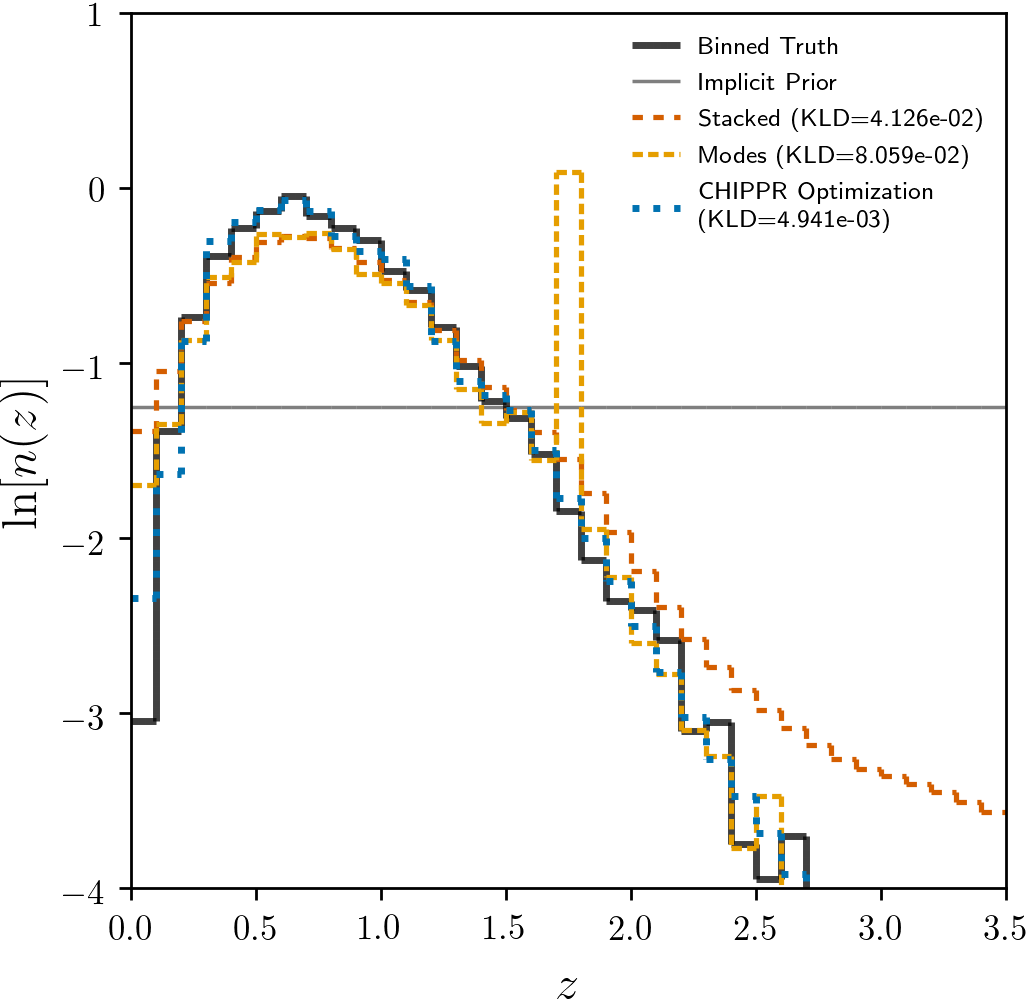
\includegraphics[width=0.5\textwidth]{figures/chippr/thesis_eout_log_estimators.png}
	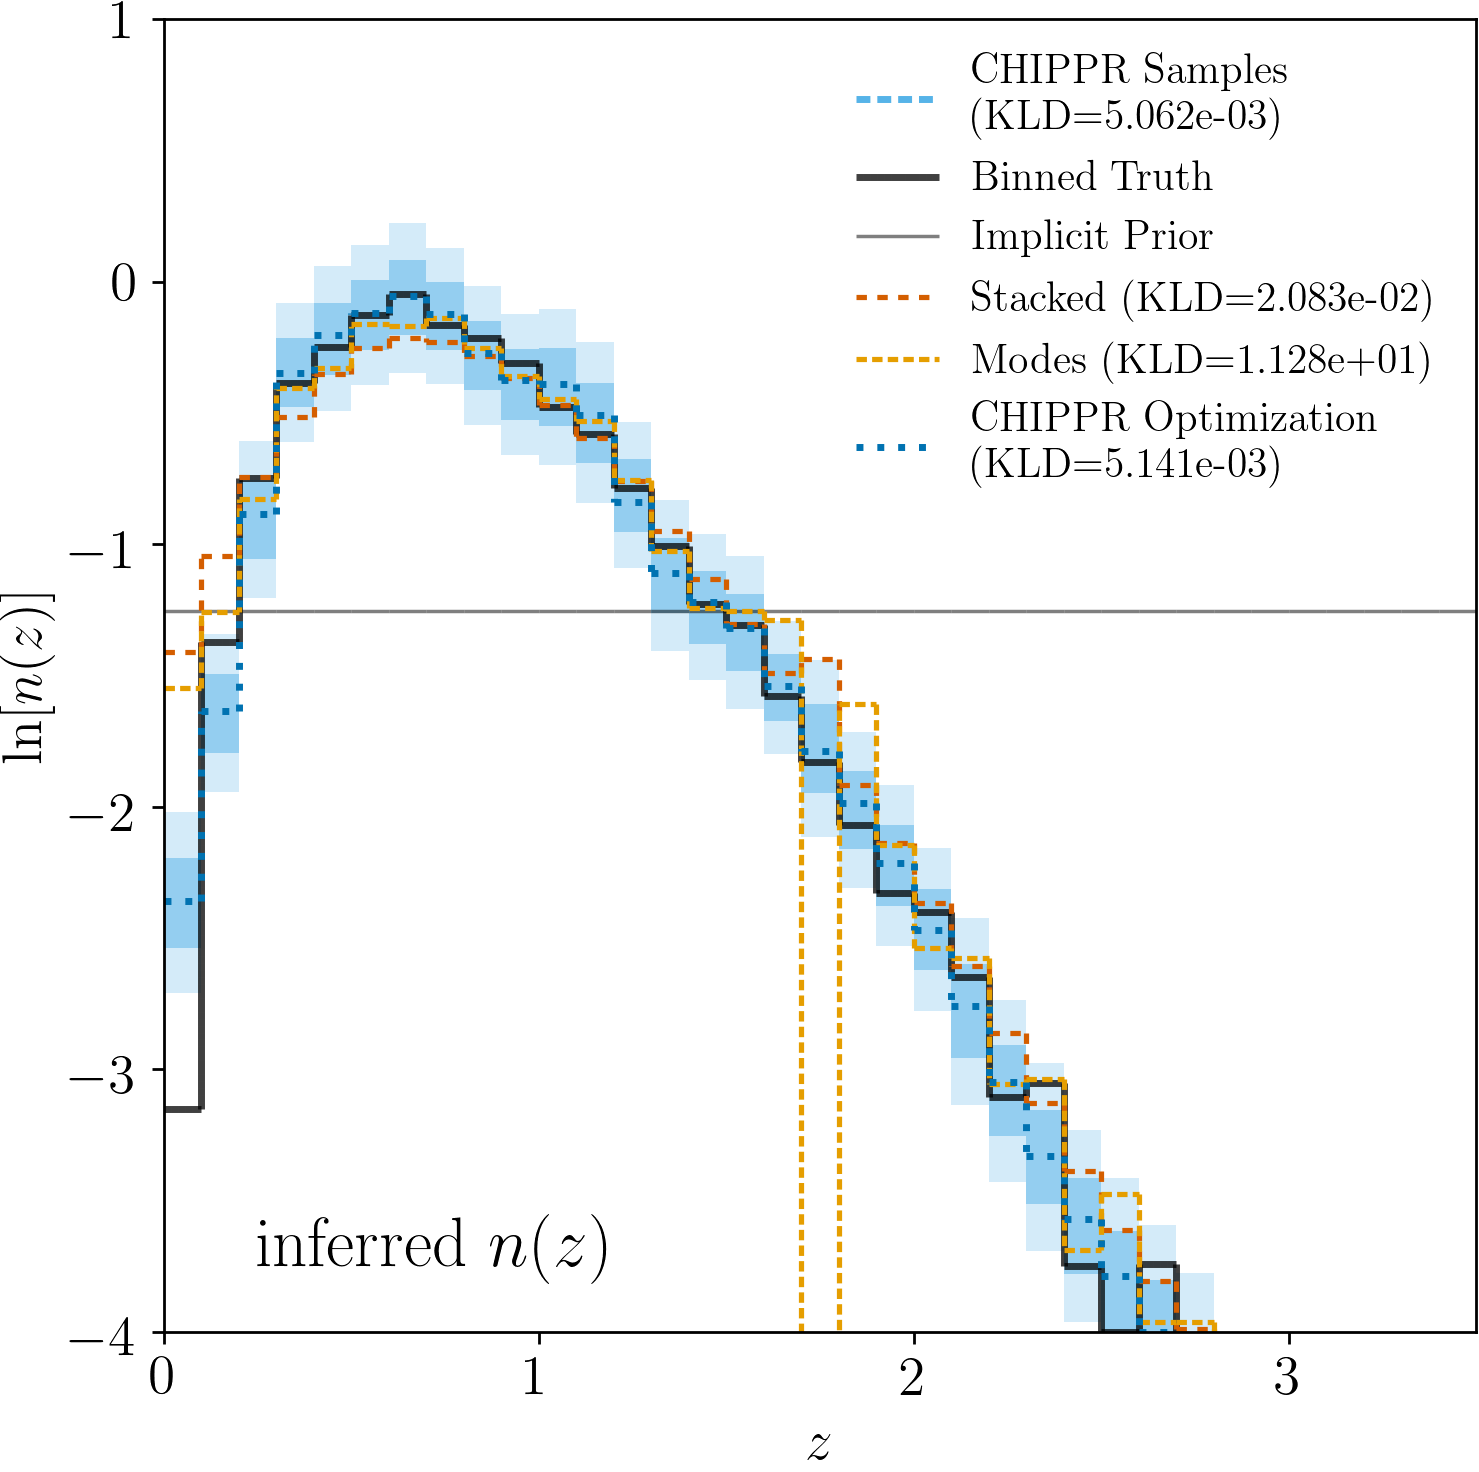
\includegraphics[width=0.5\textwidth]{figures/chippr/thesis_rout_log_estimators.png}
	\caption{
		The results of \Chippr\ (samples in light blue and optimization in dark blue) and the alternative approaches (the stacked estimator in red, the histogram of modes in yellow) on \pzpdf s with catastrophic outliers like those seen in template-fitting \pzpdf\ codes (left) and machine learning \pzpdf\ codes (right) to the \lsst\ requirements, with the true redshift density (black curve) and implicit prior (gray curve).
		Though the histogram of modes is most sensitive to a catastrophic outlier population, the stacked estimator also overestimates \nz\ under (machine learning-like outliers) and beyond (template fitting-like outliers).
	}
	\figlabel{fig:nonuniform-outliers-results}
\end{figure}

\subsection{Bias}
\sectlabel{sec:bias}

The notion of redshift bias is a form of model misspecification.

\aim{Include the tests here?
They're trivial but might be worth explaining.}

\subsection{Nontrivial implicit prior}
\sectlabel{sec:interim}

\Chippr\ can handle any implicit prior with support over the redshift range where \nz is defined, but some archetypes of implicit prior are more likely to be encountered in the wilds of \pzpdf\ codes.
Ideally, an uninformative implicit prior would be used, although it may be complicated to compute from the covariances of the raw data.  
Template-fitting codes have an explicit prior input formed by redshifting a small number of templates, leading to a highly nonuniform but physically-motivated interim prior.
%Another potential method for selecting an interim prior with support over the entire redshift range expected of the photometric survey is to sum two or more $N(z)$ distributions obtained from reliable photometric surveys in the past.  
%This is just as problematic as using a biased spectroscopically derived $N(z)$ as the interim prior because the sum of redshift distributions for two or more surveys does not reflect our beliefs about the true distribution for a single survey even though it provides support over the same redshift range.  
%To simulate this case, we choose an interim prior with more weight at high and low redshifts than for mid-range redshifts.  
Machine learning approaches tend to be trained on previously observed data sets that are biased towards low redshift, which biases the implicit prior towards low redshift.
Some efforts have been made to modify an observationally informed implicit prior so that it is more representative of the photometric data for which redshifts are desired \citep{Sheldon2012}, but, unless it is equal to the true \nz, it will propagate to the results of traditional \nz\ estimation methods.  
%Because low-redshift galaxies are more likely to be bright enough to be observed by such a survey, $N(z)$ determined from that sample may be heavily biased to low redshift galaxies.  
%By contrast, the galaxies that were unobserved in such a survey are more likely be dimmer, making them more likely to be at higher redshifts.  
%Since the interim prior is not compatible with our beliefs about the true redshift distribution, the resulting interim redshift posteriors will be inappropriate.  

\Fig{fig:pzs-priors} shows examples of \pzpdf s with a low-redshift favoring implicit prior emulating that of a machine learning approach to \pz\ estimation and a more complex interim prior emulating that of a template-fitting \pz\ method.
One can see that the \pzpdf s take different shapes from one another even though the marginal histograms are identical.

\begin{figure}
	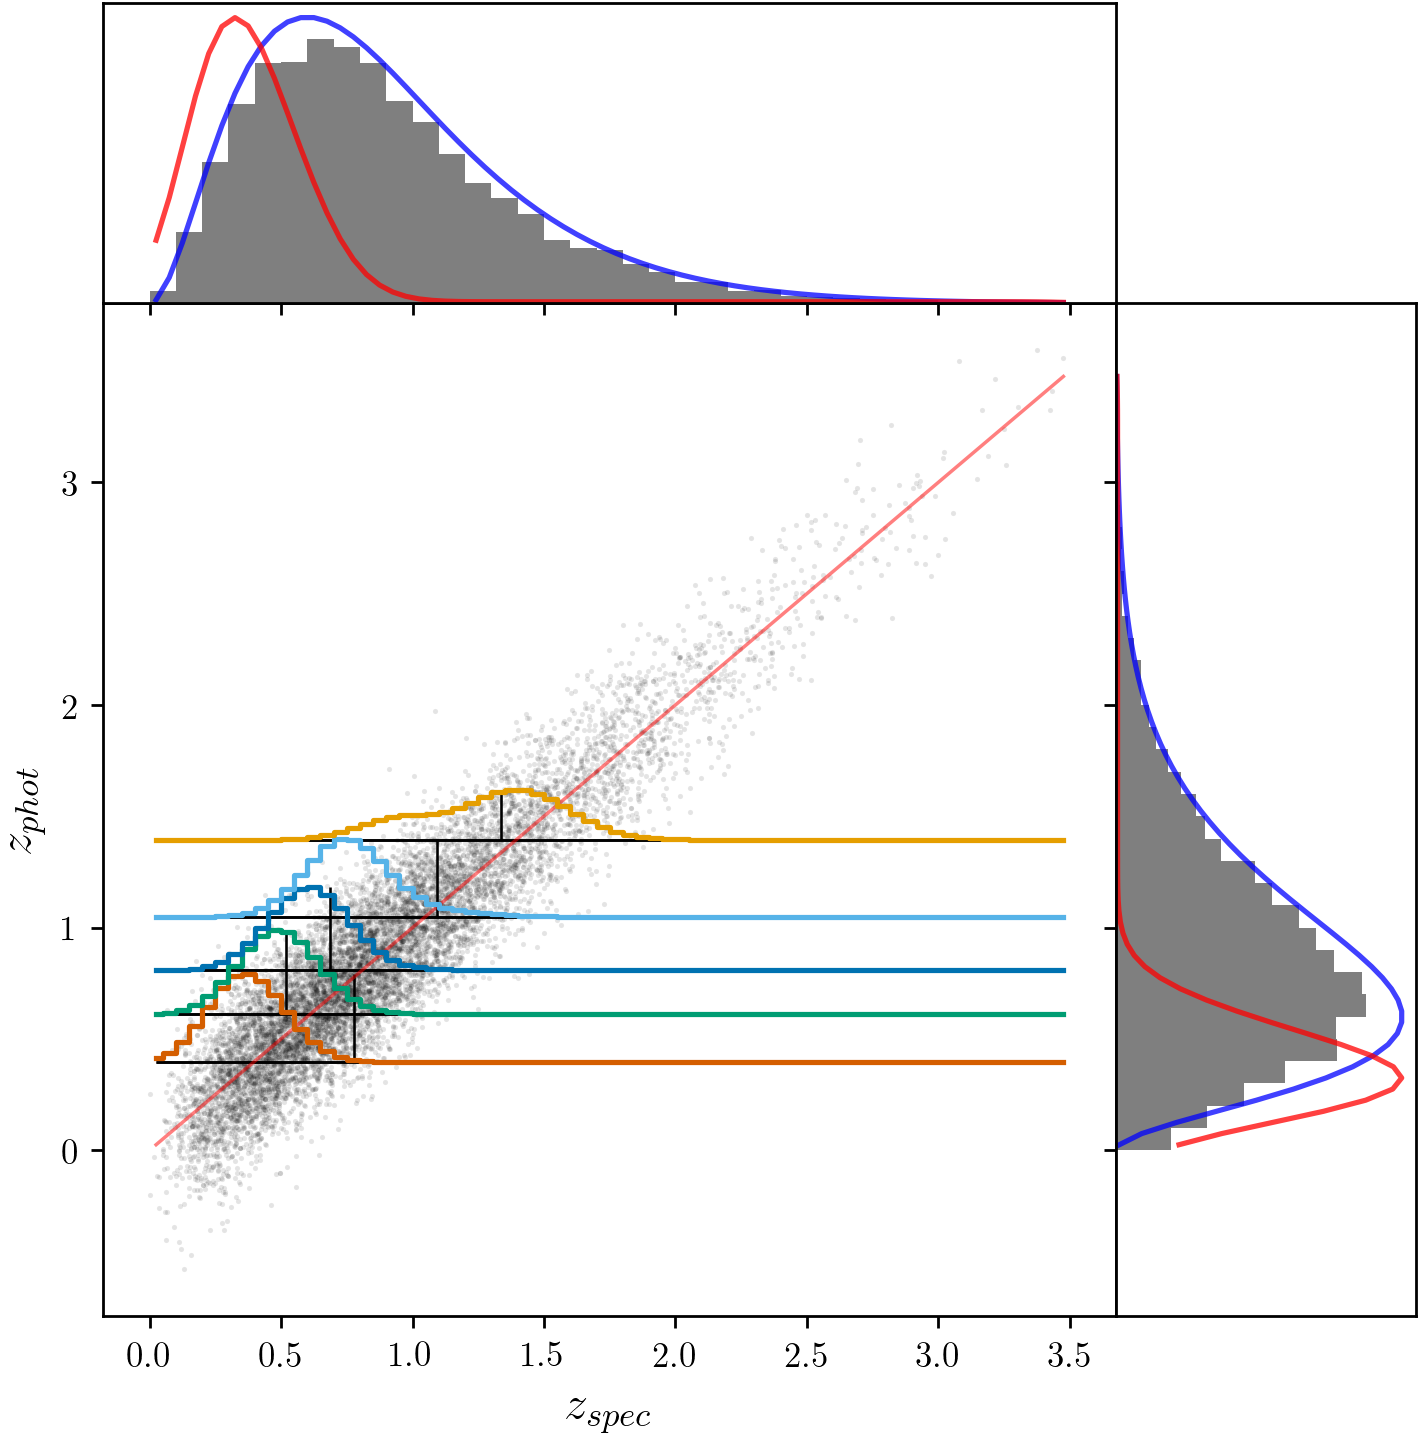
\includegraphics[width=0.5\textwidth]{figures/chippr/samplepzs_trpr.png}
	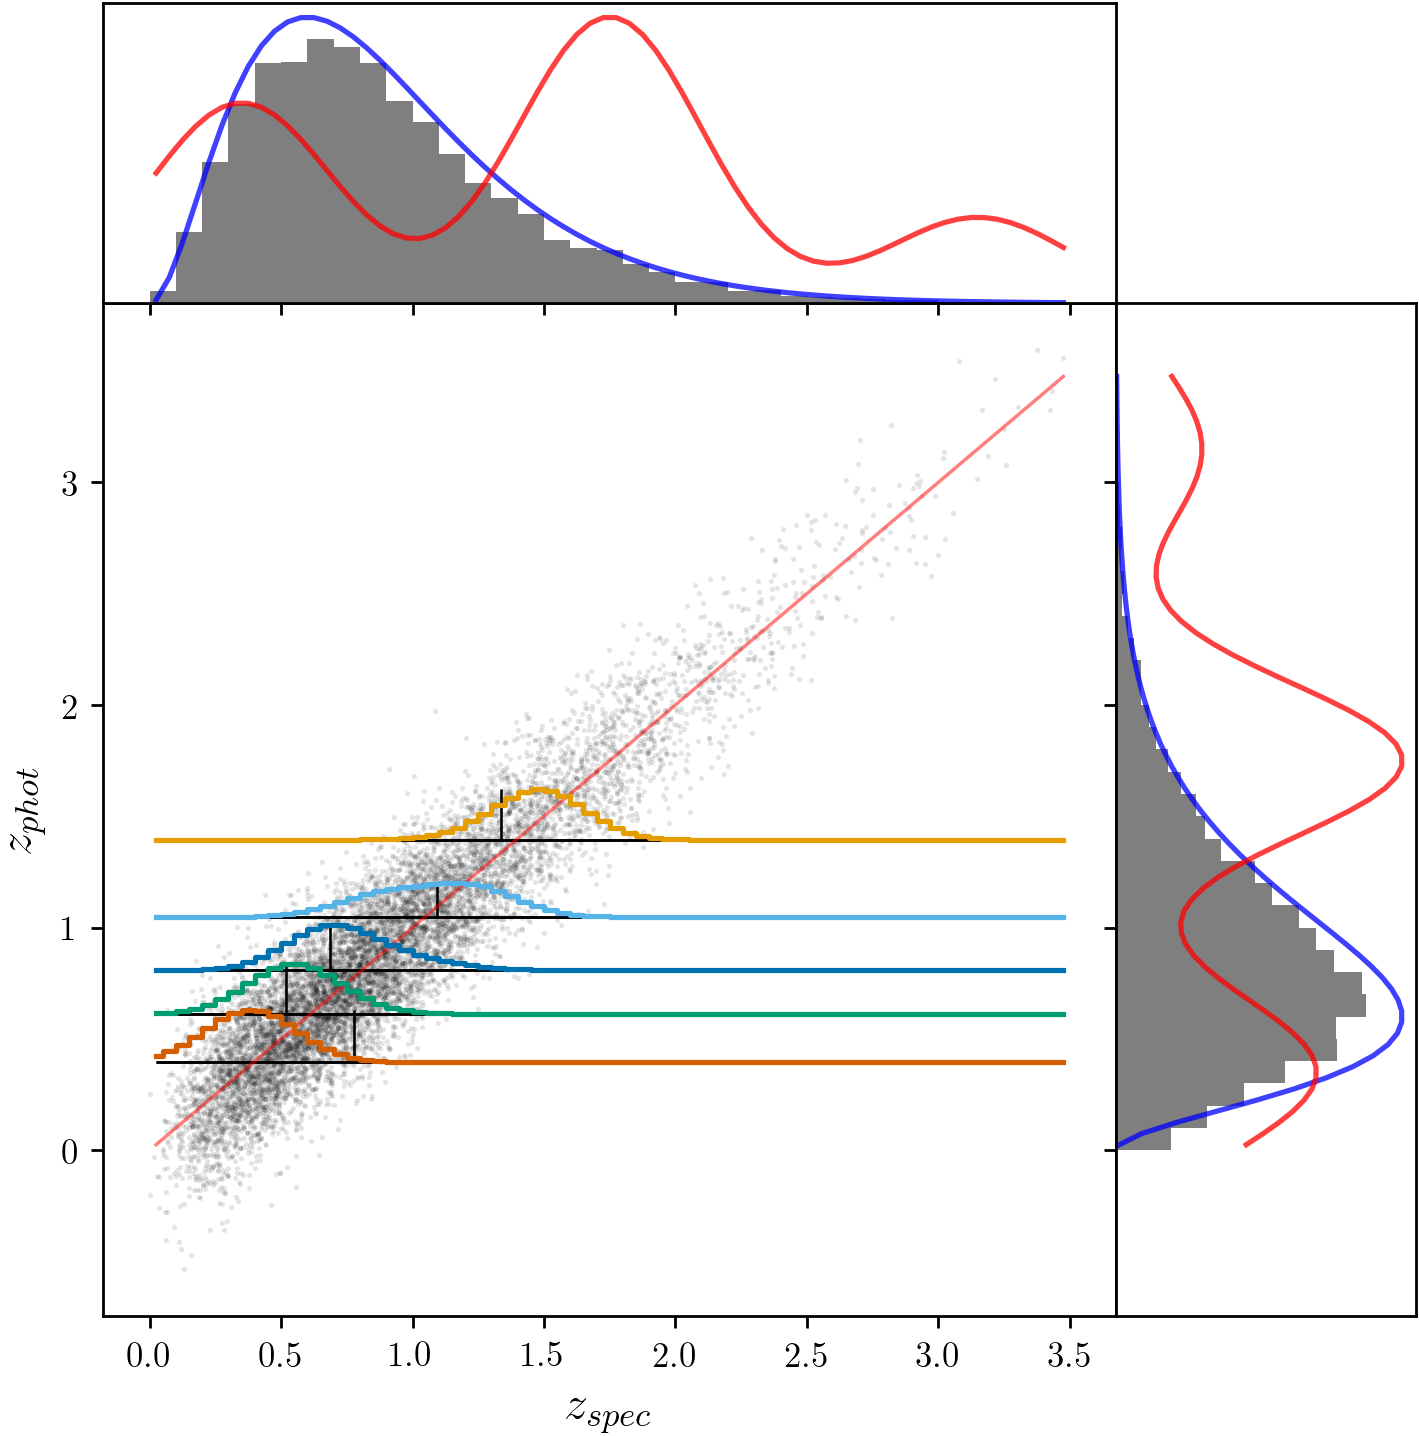
\includegraphics[width=0.5\textwidth]{figures/chippr/samplepzs_tmpr.png}
	\caption{
		Examples of mock \pzpdf s (colored lines) generated with a machine learning-like implicit prior (left) and a template-fitting-like implicit prior (right), including samples from the probability space of true and observed redshift (black points), \pzpdf s (colored lines), the true redshifts of the example \pzpdf s (black vertical lines).
		A histogram (gray) of points in each dimension is shown in the respective inset, with the true redshift distribution (blue curve) and implicit prior (red curve).
	}
	\figlabel{fig:pzs-priors}
\end{figure}

\Fig{fig:results-priors} shows the performance of \Chippr\ and the traditional methods on \pzpdf s generated with nontrivial implicit priors.
In both cases, the \Chippr\ \mmle\ effectively recovers the true redshift distribution.
The alternatives, however, are biased by the implicit prior except where it is flat, in the case of high redshifts for the machine learning-like implicit prior.
\aim{Show that this gets worse for higher intrinsic scatter as well?}

\begin{figure}
	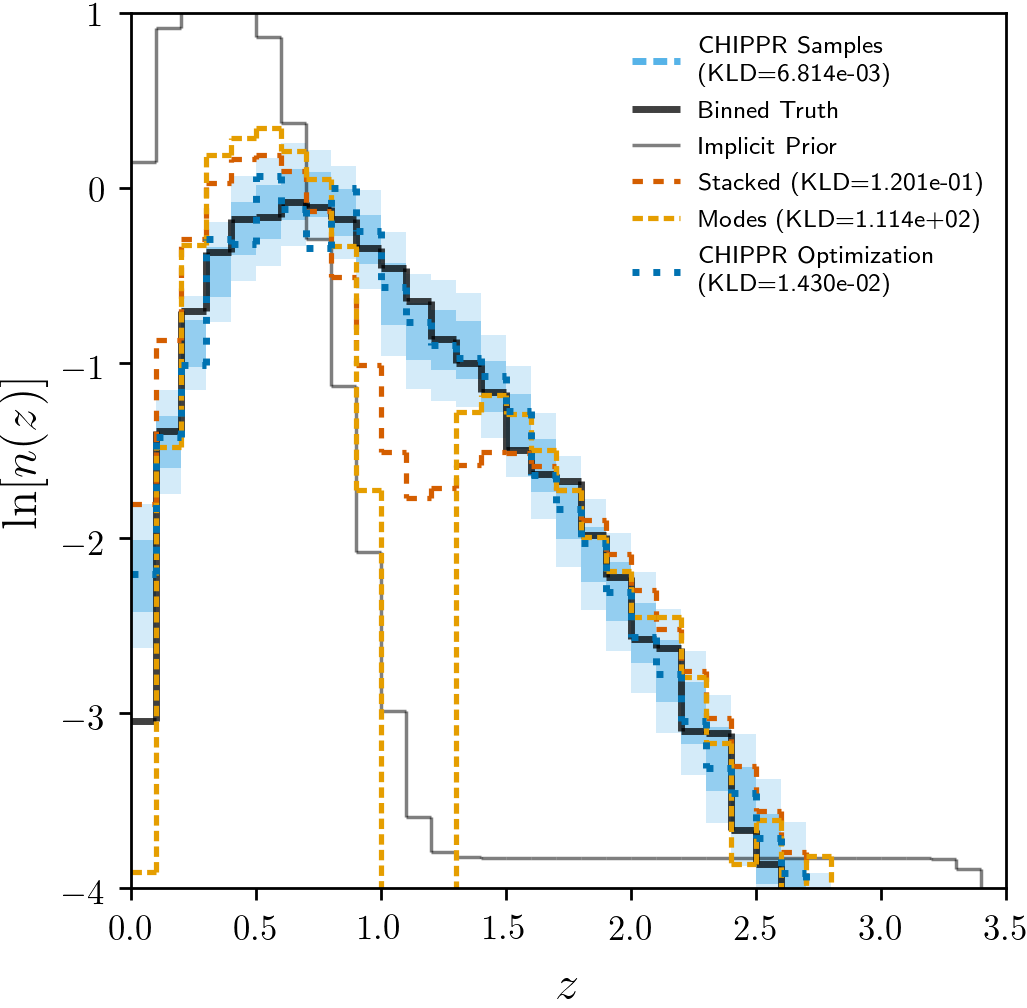
\includegraphics[width=0.5\textwidth]{figures/chippr/results_trpr.png}
	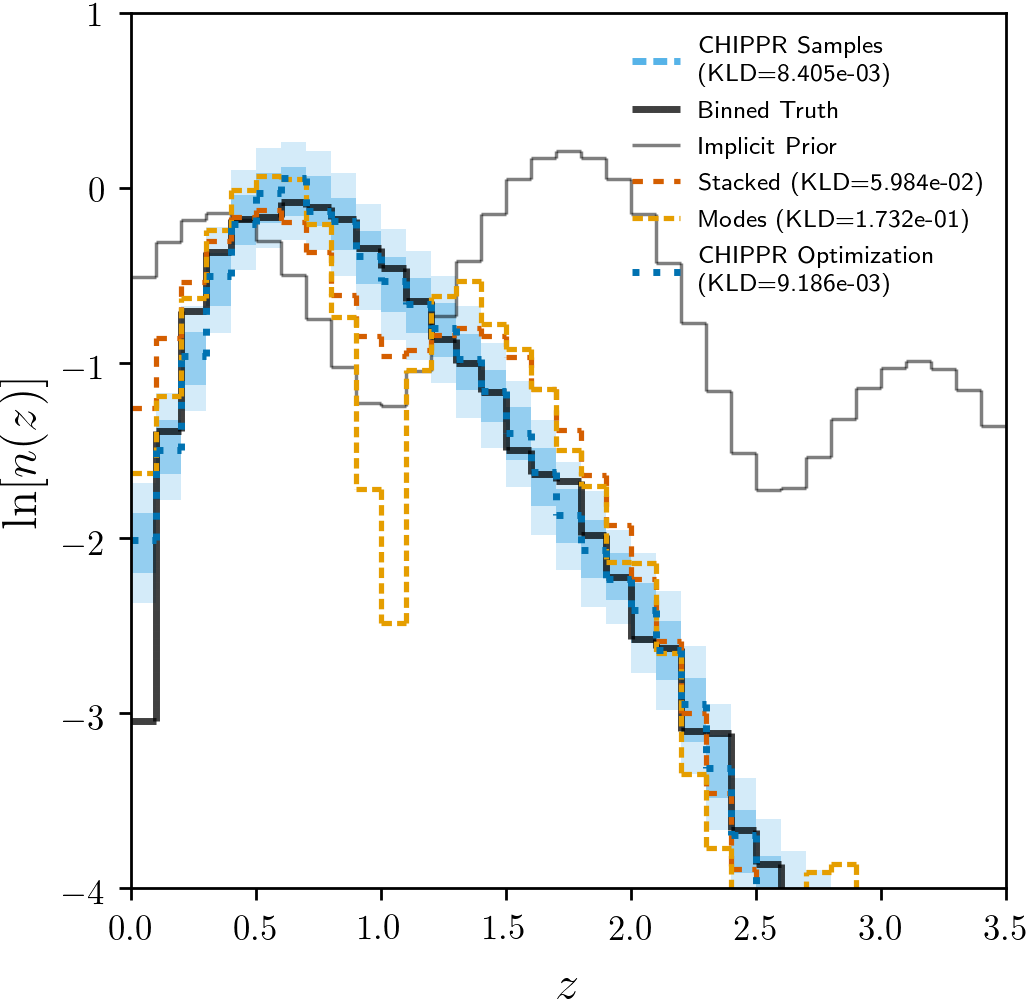
\includegraphics[width=0.5\textwidth]{figures/chippr/results_tmpr.png}
	\caption{
		The results of \Chippr\ (samples in light blue and optimization in dark blue) and the alternative approaches (the stacked estimator in red and the histogram of modes in yellow) on \pzpdf s with an implicit prior like that of machine learning \pzpdf\ approaches (left) and an implicit prior like that of template-fitting \pzpdf\ codes (right), with the true redshift density (black curve) and implicit prior (gray curve).
		\Chippr\ is robust to a nontrivial implicit prior, but the alternatives are biased toward the implicit prior.
	}
	\figlabel{fig:results-priors}
\end{figure}

\section{Discussion}
\sectlabel{sec:results}

\aim{I still need to write the intro to the big LSST-like forecast and incorrect implicit prior sections.}

\aim{Q: How does the result of \chippr\ compare to established estimators in terms of the accuracy of $n(z)$?\\
	A: \chippr\ yields the best possible $n(z)$, conditional on the accuracy of the photo-$z$ PDFs used.}

\aim{Include quantitative results on KLD of \Nz\ and cosmological parameter space.}

\subsection{LSST Requirements}
\sectlabel{sec:lsstdemo}

The \lsst\ Science Requirements Document (SRD)\footnote{\url{https://docushare.lsstcorp.org/docushare/dsweb/Get/LPM-17}} states that the main cosmological sample of $\sim 10^{7}$ galaxies must have \pz s satisfying root-mean-square error $\sigma_z < 0.02 (1+z)$, $3 \sigma$ catastrophic outlier rate $< 10\%$, and bias $< 0.003$.
To test the impact of these uncertainties, we simulated mock data with all three effects and did a Fisher matrix forecast using \cosmolike.
\aim{Cite CosmoLike.}

Using 35 evenly spaced tomographic bins $0.0101 < z < 3.4101$,  

\begin{figure*}
	\begin{center}
		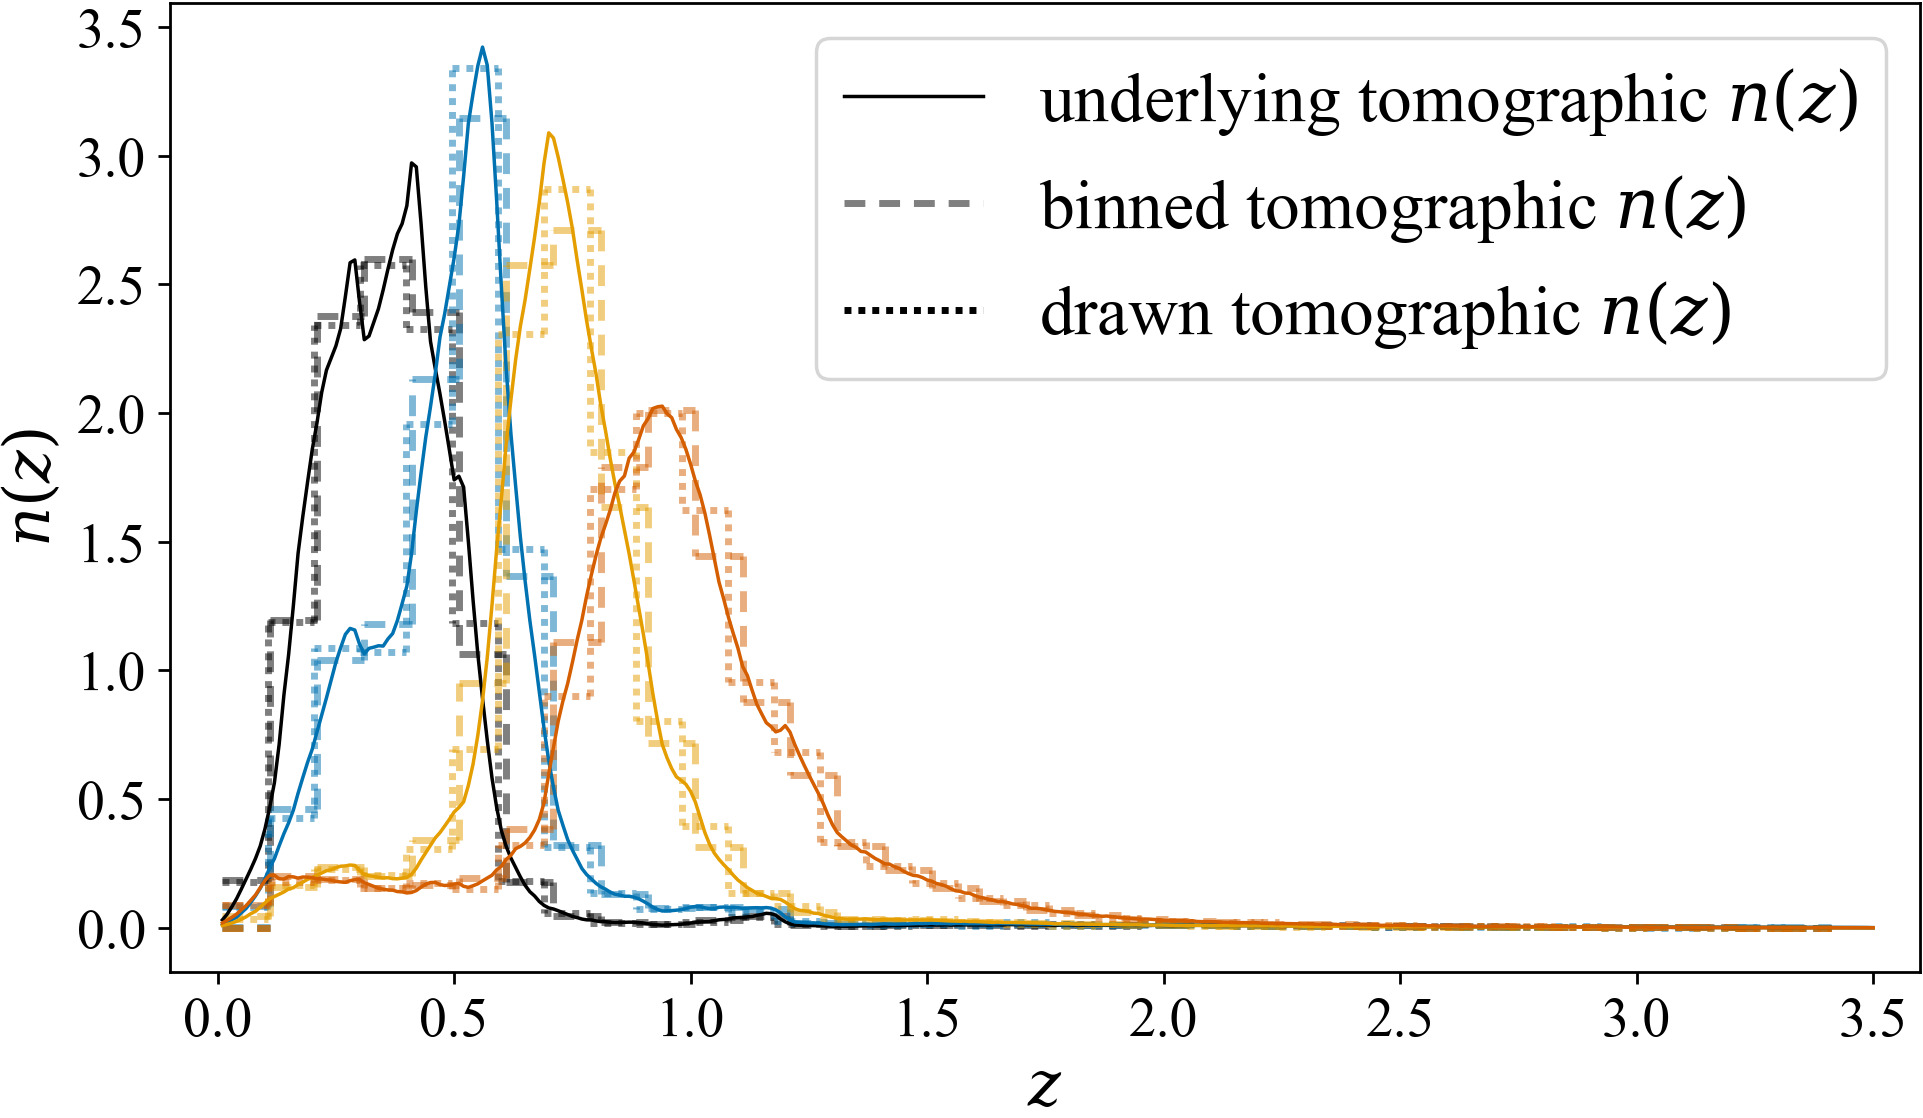
\includegraphics[width=\textwidth]{figures/chippr/cosmolike_inputs.png}
		\caption{The underlying, drawn, and binned, \nz\ for the four tomographic bins.}
		\figlabel{fig:lsstdemo}
	\end{center}
\end{figure*}

\begin{figure*}
	\begin{center}
		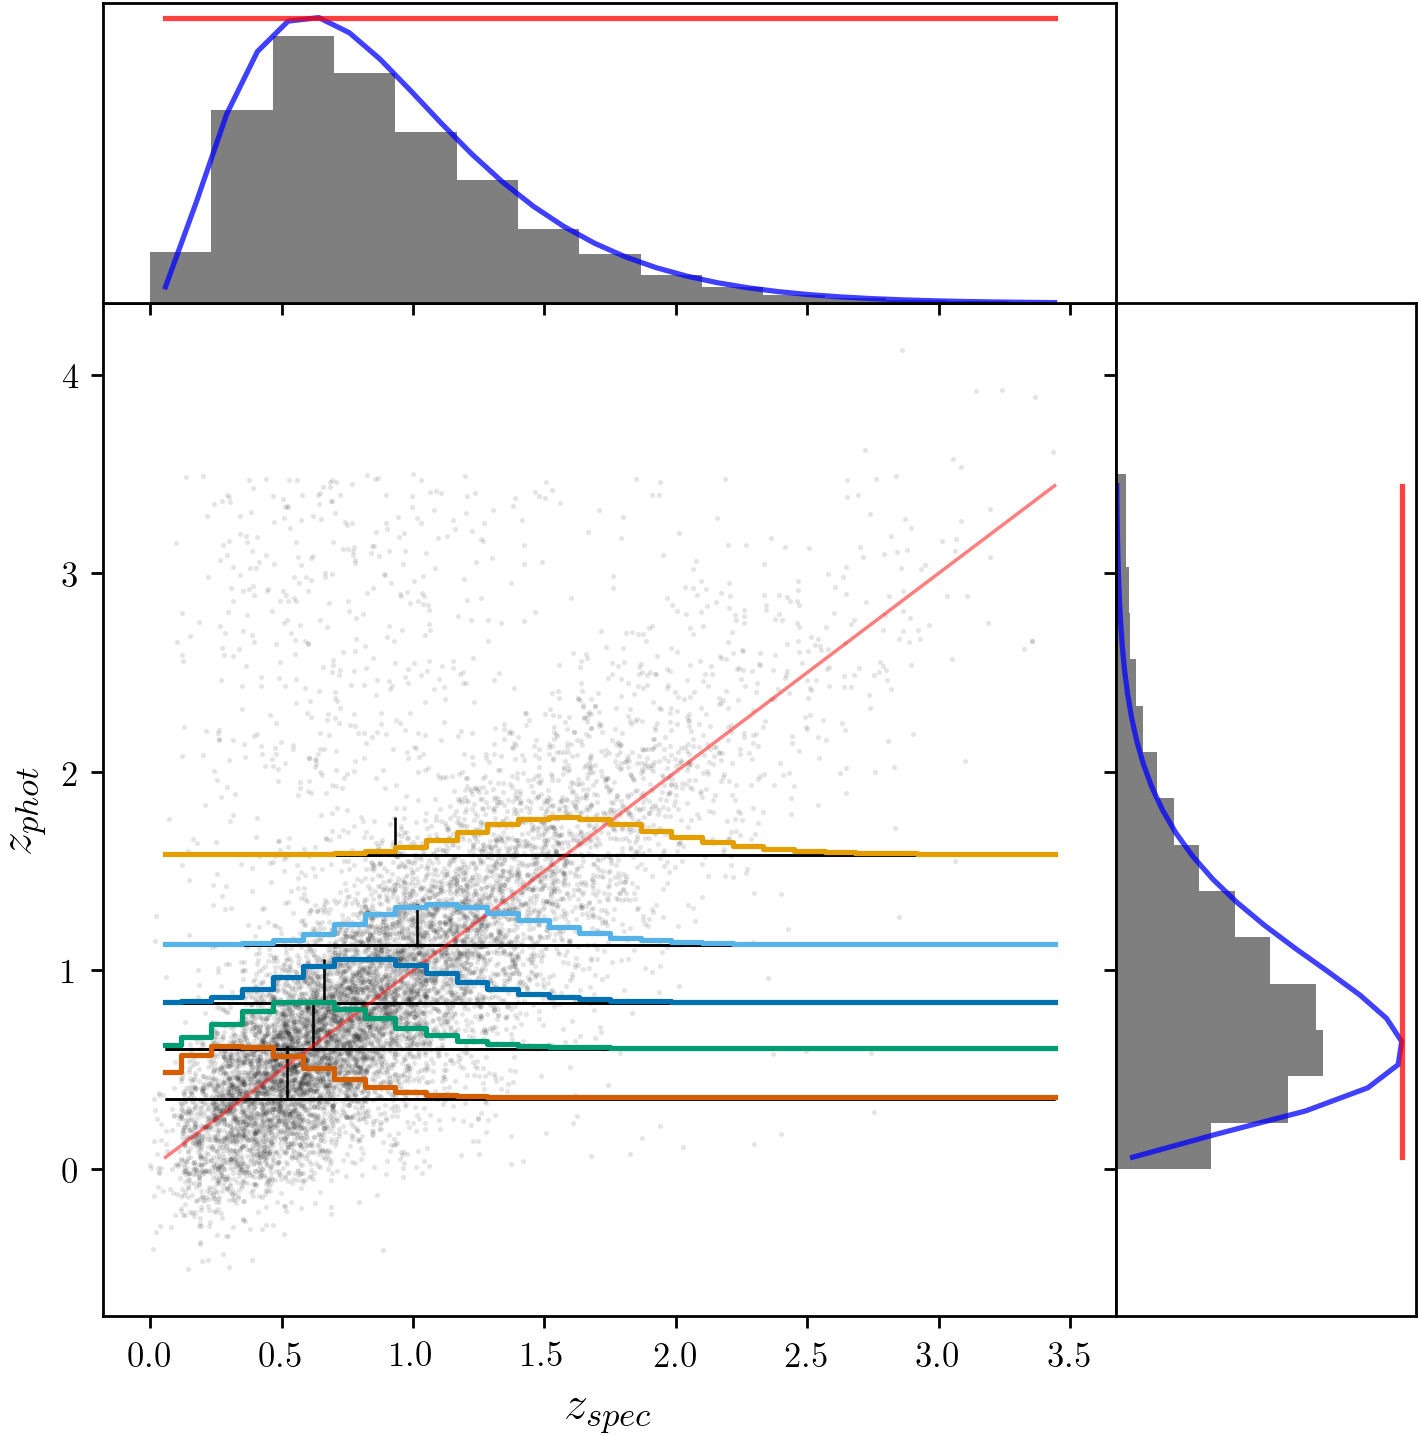
\includegraphics[width=0.45\textwidth]{figures/chippr/lsst_scatter.png}
		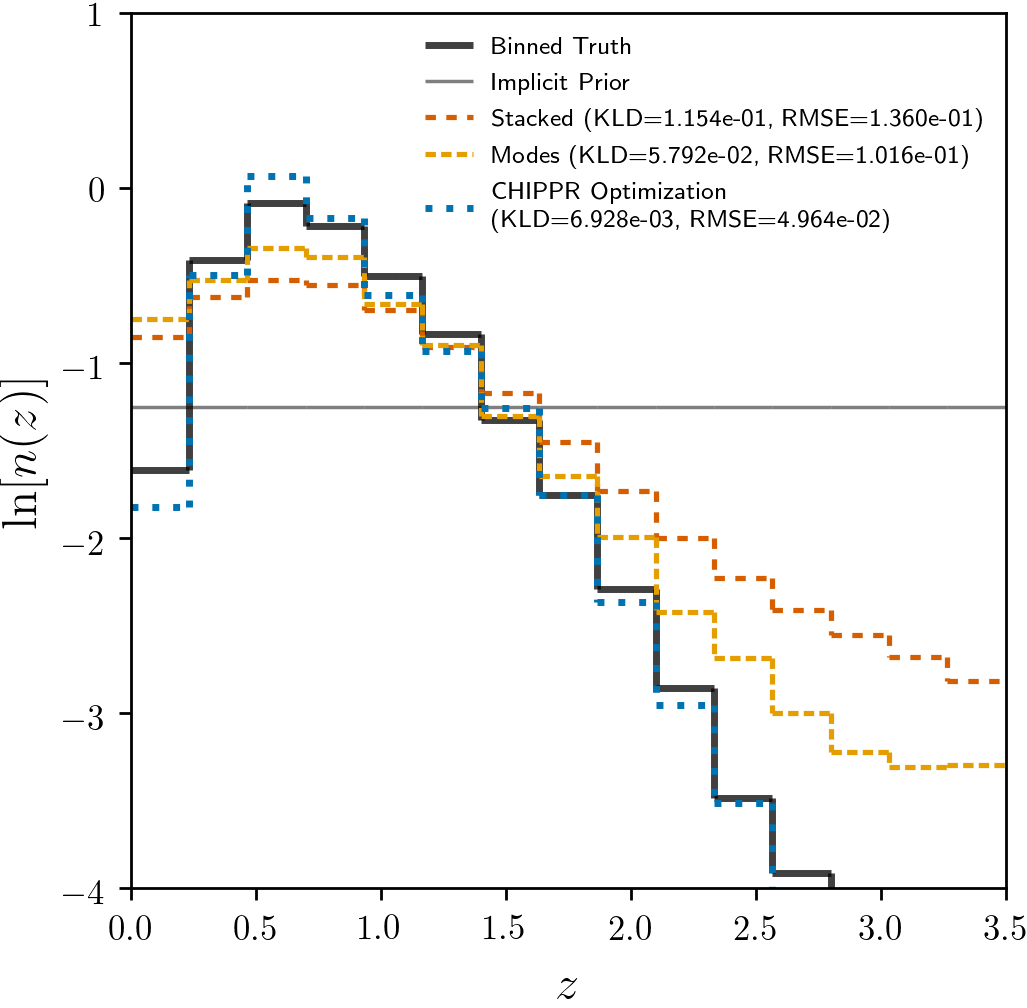
\includegraphics[width=0.45\textwidth]{figures/chippr/lsst_log_estimators.png}
		\caption{T
		\aim{Rerun this with 35 bins and sampling to match other figures.}}
		\figlabel{fig:lsstdemo}
	\end{center}
\end{figure*}

It is of interest to explore the impact of incorrectly estimated \nz\ on the inference of the cosmological parameters to answer the question of how wrong we will be in our understanding of the universe if we don't perform a valid inference.
To find an answer, I considered a set of tomographically binned \nz\ and cosmological parameter covariance matrices used for \desc\ forecasting, for which the true \nz\ in each pre-defined bin is already provided in the form of an evaluation of a function on a fine grid of $350$ redshifts $0.0101 < z < 3.5001$.
First, I binned them down to a piecewise constant parameterization with a manageable $35$ parameters for \chippr's sampling capabilities.
Next, I drew $10^{4}$ true redshifts from the binned true \nz\ for each tomographic bin.
The original, binned, and drawn \nz\ are shown in \Fig{fig:tomobins}

\begin{figure*}
	\begin{center}
		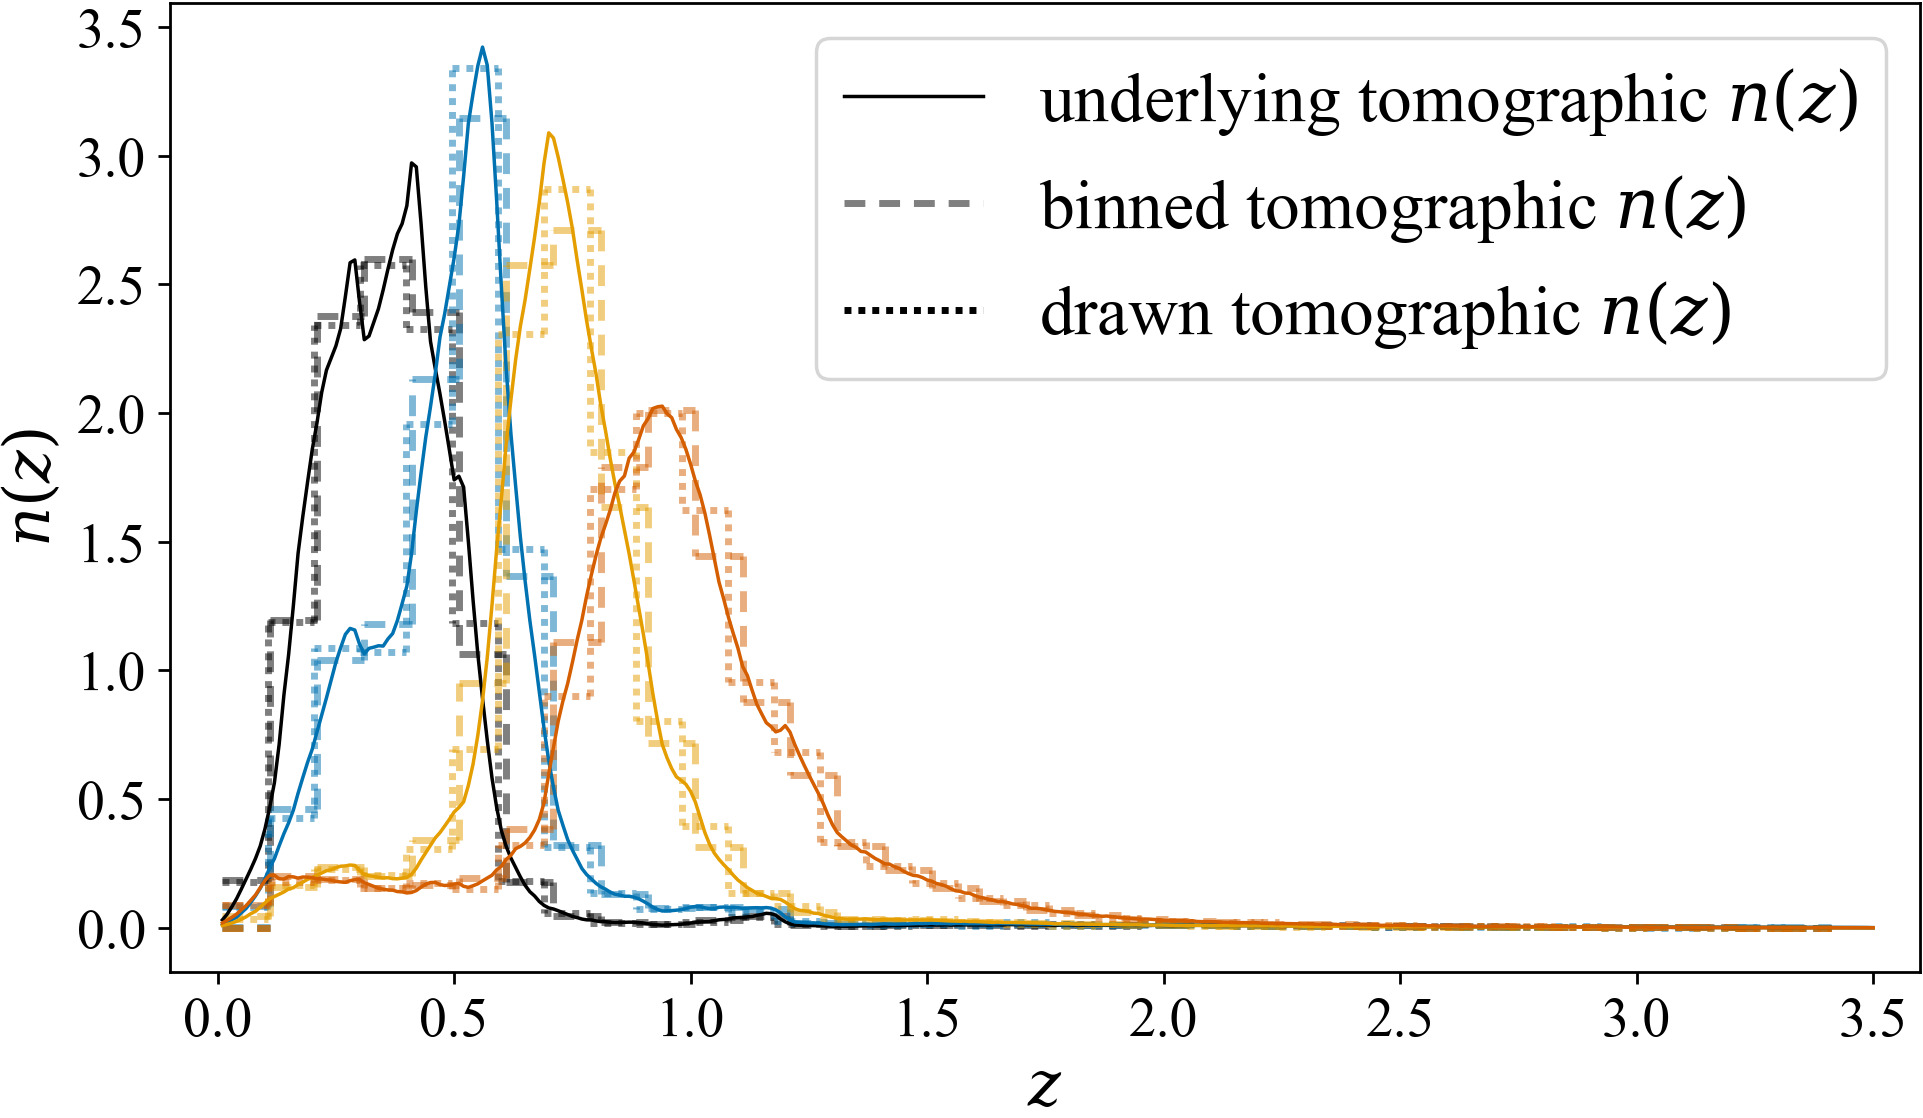
\includegraphics[width=0.99\textwidth]{figures/chippr/cosmolike_inputs.png}
		\caption{The \lsst-like tomographic binning and true redshift distribution, where the truth (solid) is a PDF evaluated on a fine grid of $350$ redshifts $0.0101 < z < 3.5001$, and the binned (dashed) and drawn (dotted) \nz\ are piecewise constant functions evaluated in $35$ evenly spaced bins.
		}
		\figlabel{fig:tomobins}
	\end{center}
\end{figure*}

Using the \lsst\ \pz\ requirements given in \Sect{sec:lsstdemo}, I emulated \pzpdf s corresponding to the $10^{4}$ true redshifts drawn from the true \nz\ in each bin using the procedure of \Fig{fig:flowchart}.
I then ran \chippr\ as well as the two other \nz\ estimation methods on the \pzpdf\ catalog for each tomographic bin.
The estimates are given in \Fig{fig:per-bin-ests}.
One can see that the excessive breadth of the stacked estimator and the histogram of the modes of the \pzpdf s.

\begin{figure*}
	\begin{center}
		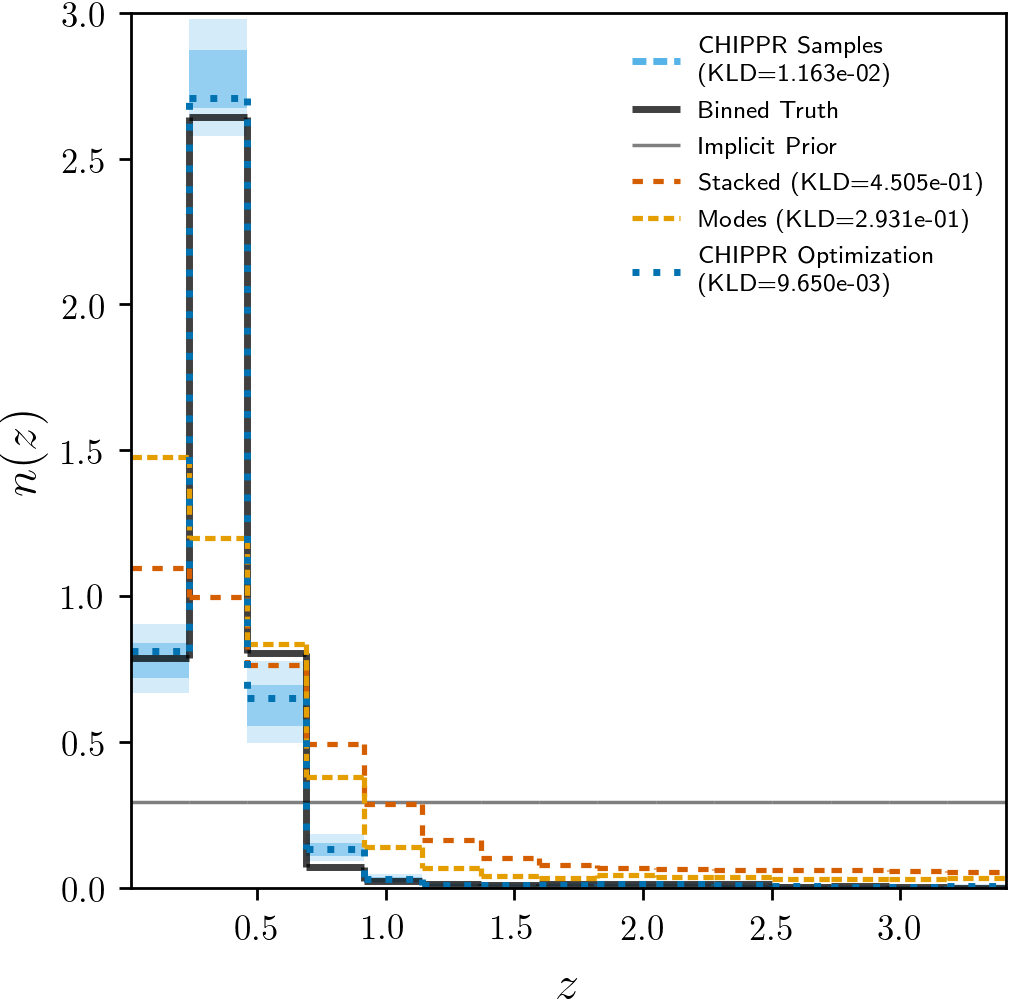
\includegraphics[width=0.24\textwidth]{figures/chippr/0single_lsst_lin_estimators.png}
		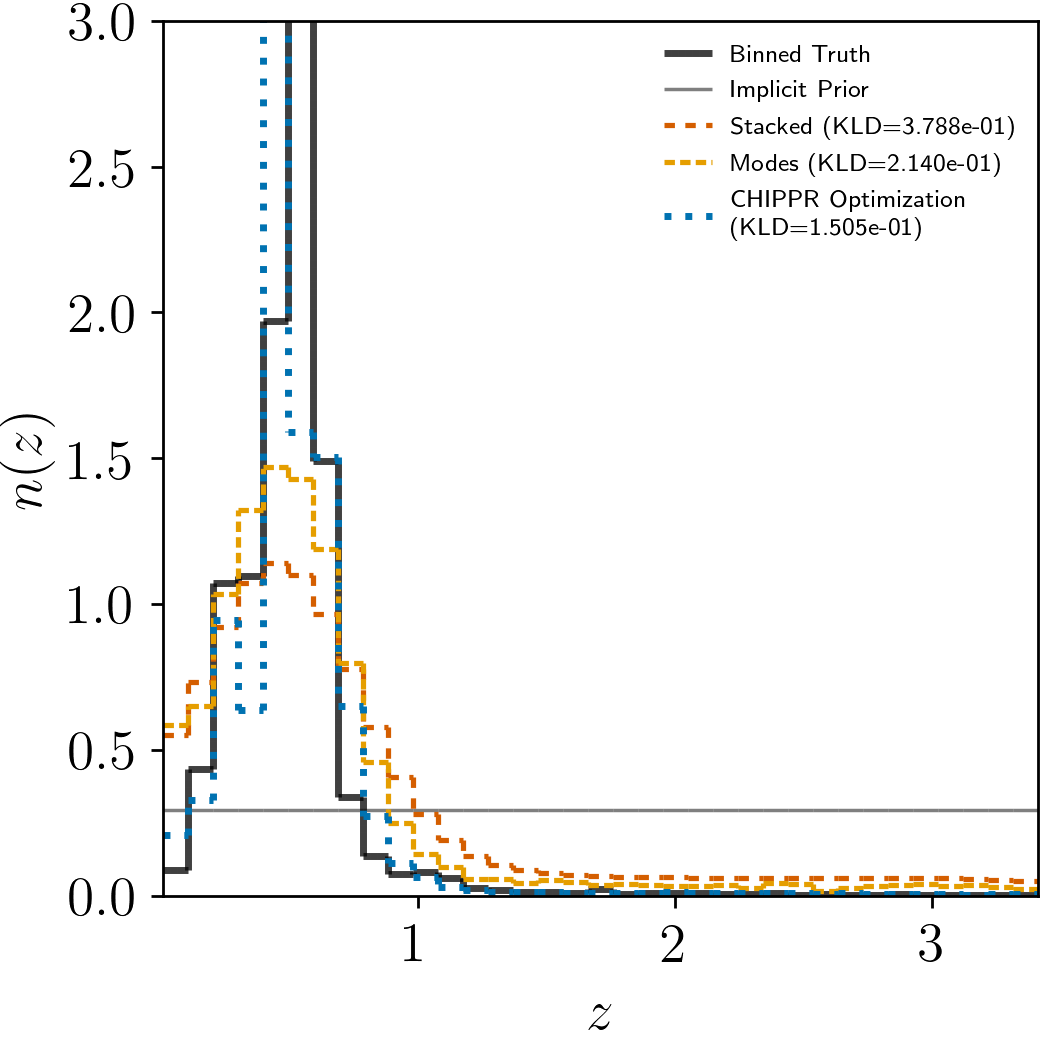
\includegraphics[width=0.24\textwidth]{figures/chippr/1single_lsst_lin_estimators.png}		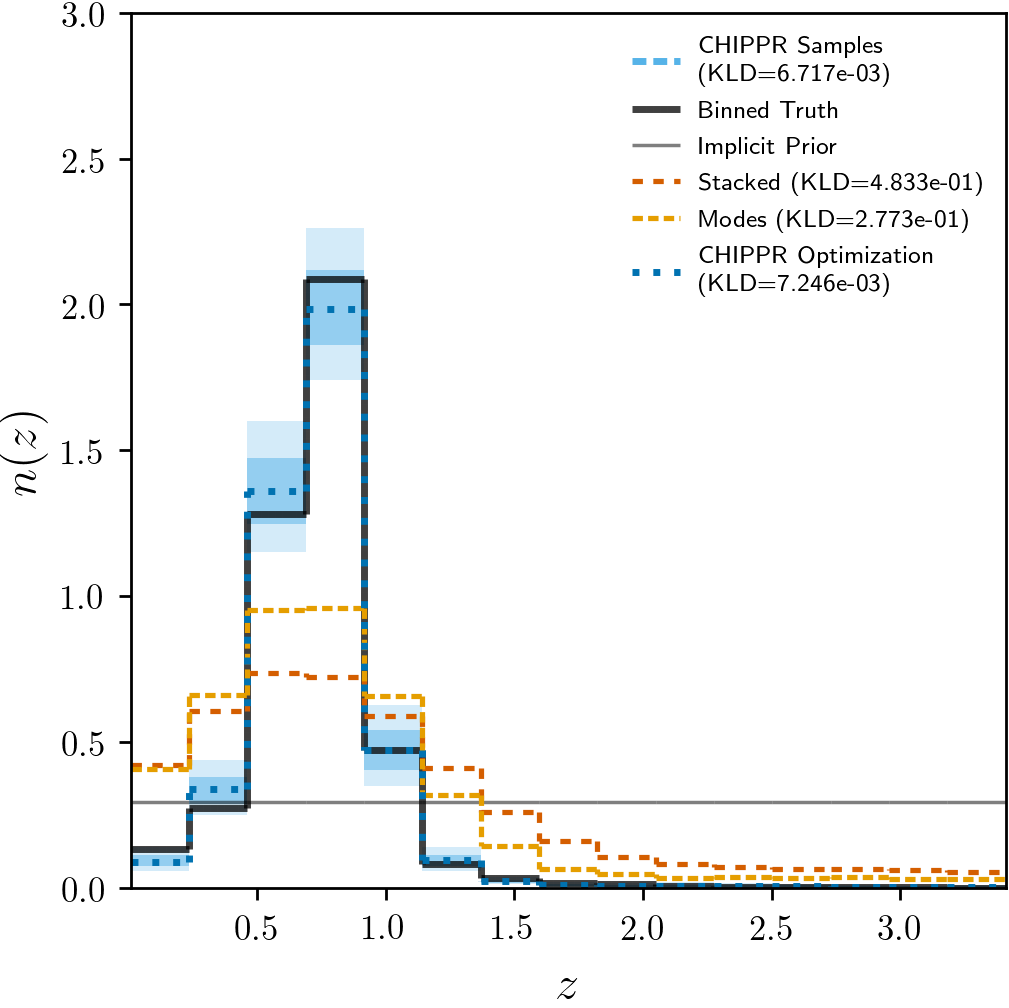
\includegraphics[width=0.24\textwidth]{figures/chippr/2single_lsst_lin_estimators.png}
		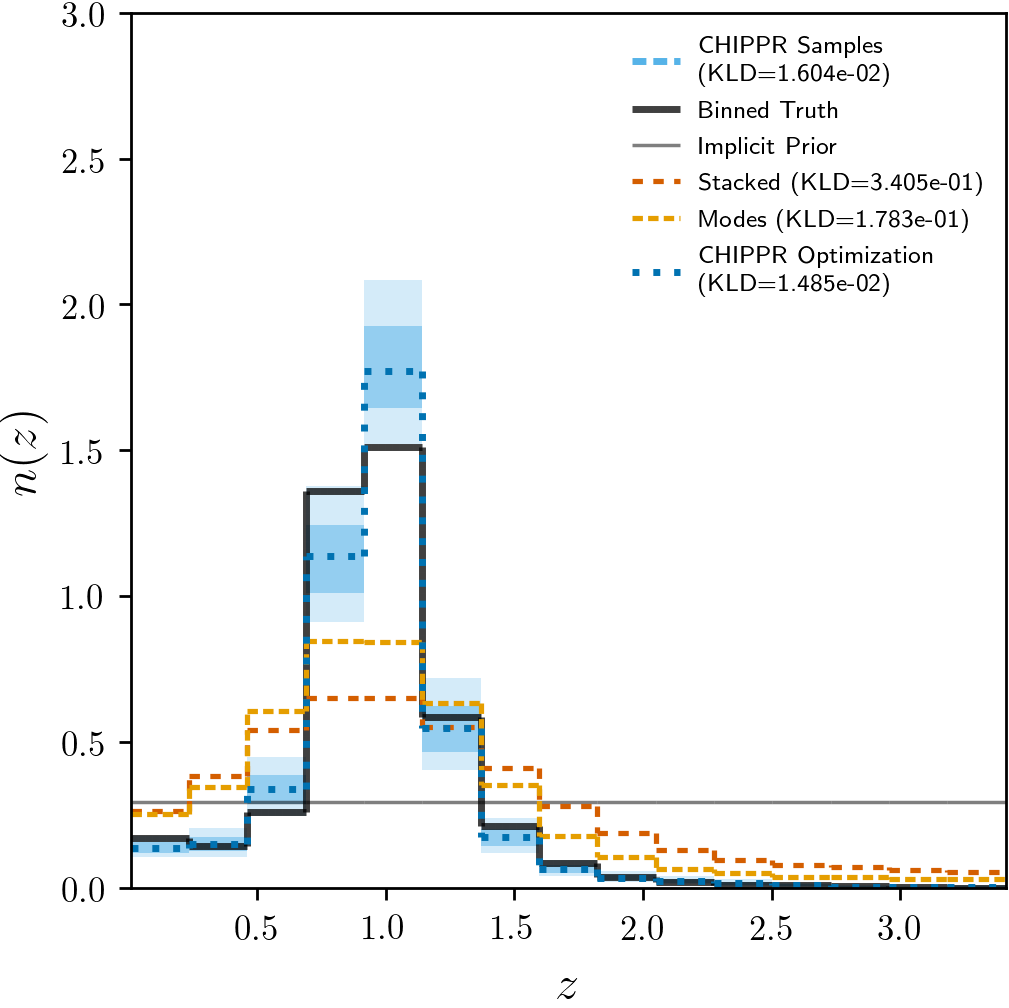
\includegraphics[width=0.24\textwidth]{figures/chippr/3single_lsst_lin_estimators.png}
		\caption{The \chippr-derived and other estimators of \nz\ in each tomographic bin.
		\aim{Make this one big plot instead of four little ones to eliminate repeated axis labels and legend.}}
		\figlabel{fig:per-bin-ests}
	\end{center}
\end{figure*}

I then used the different estimators of \nz\ in a cosmological forecasting procedure with \cosmolike.
\aim{Cite Krause here.}

\begin{figure*}
	\begin{center}
		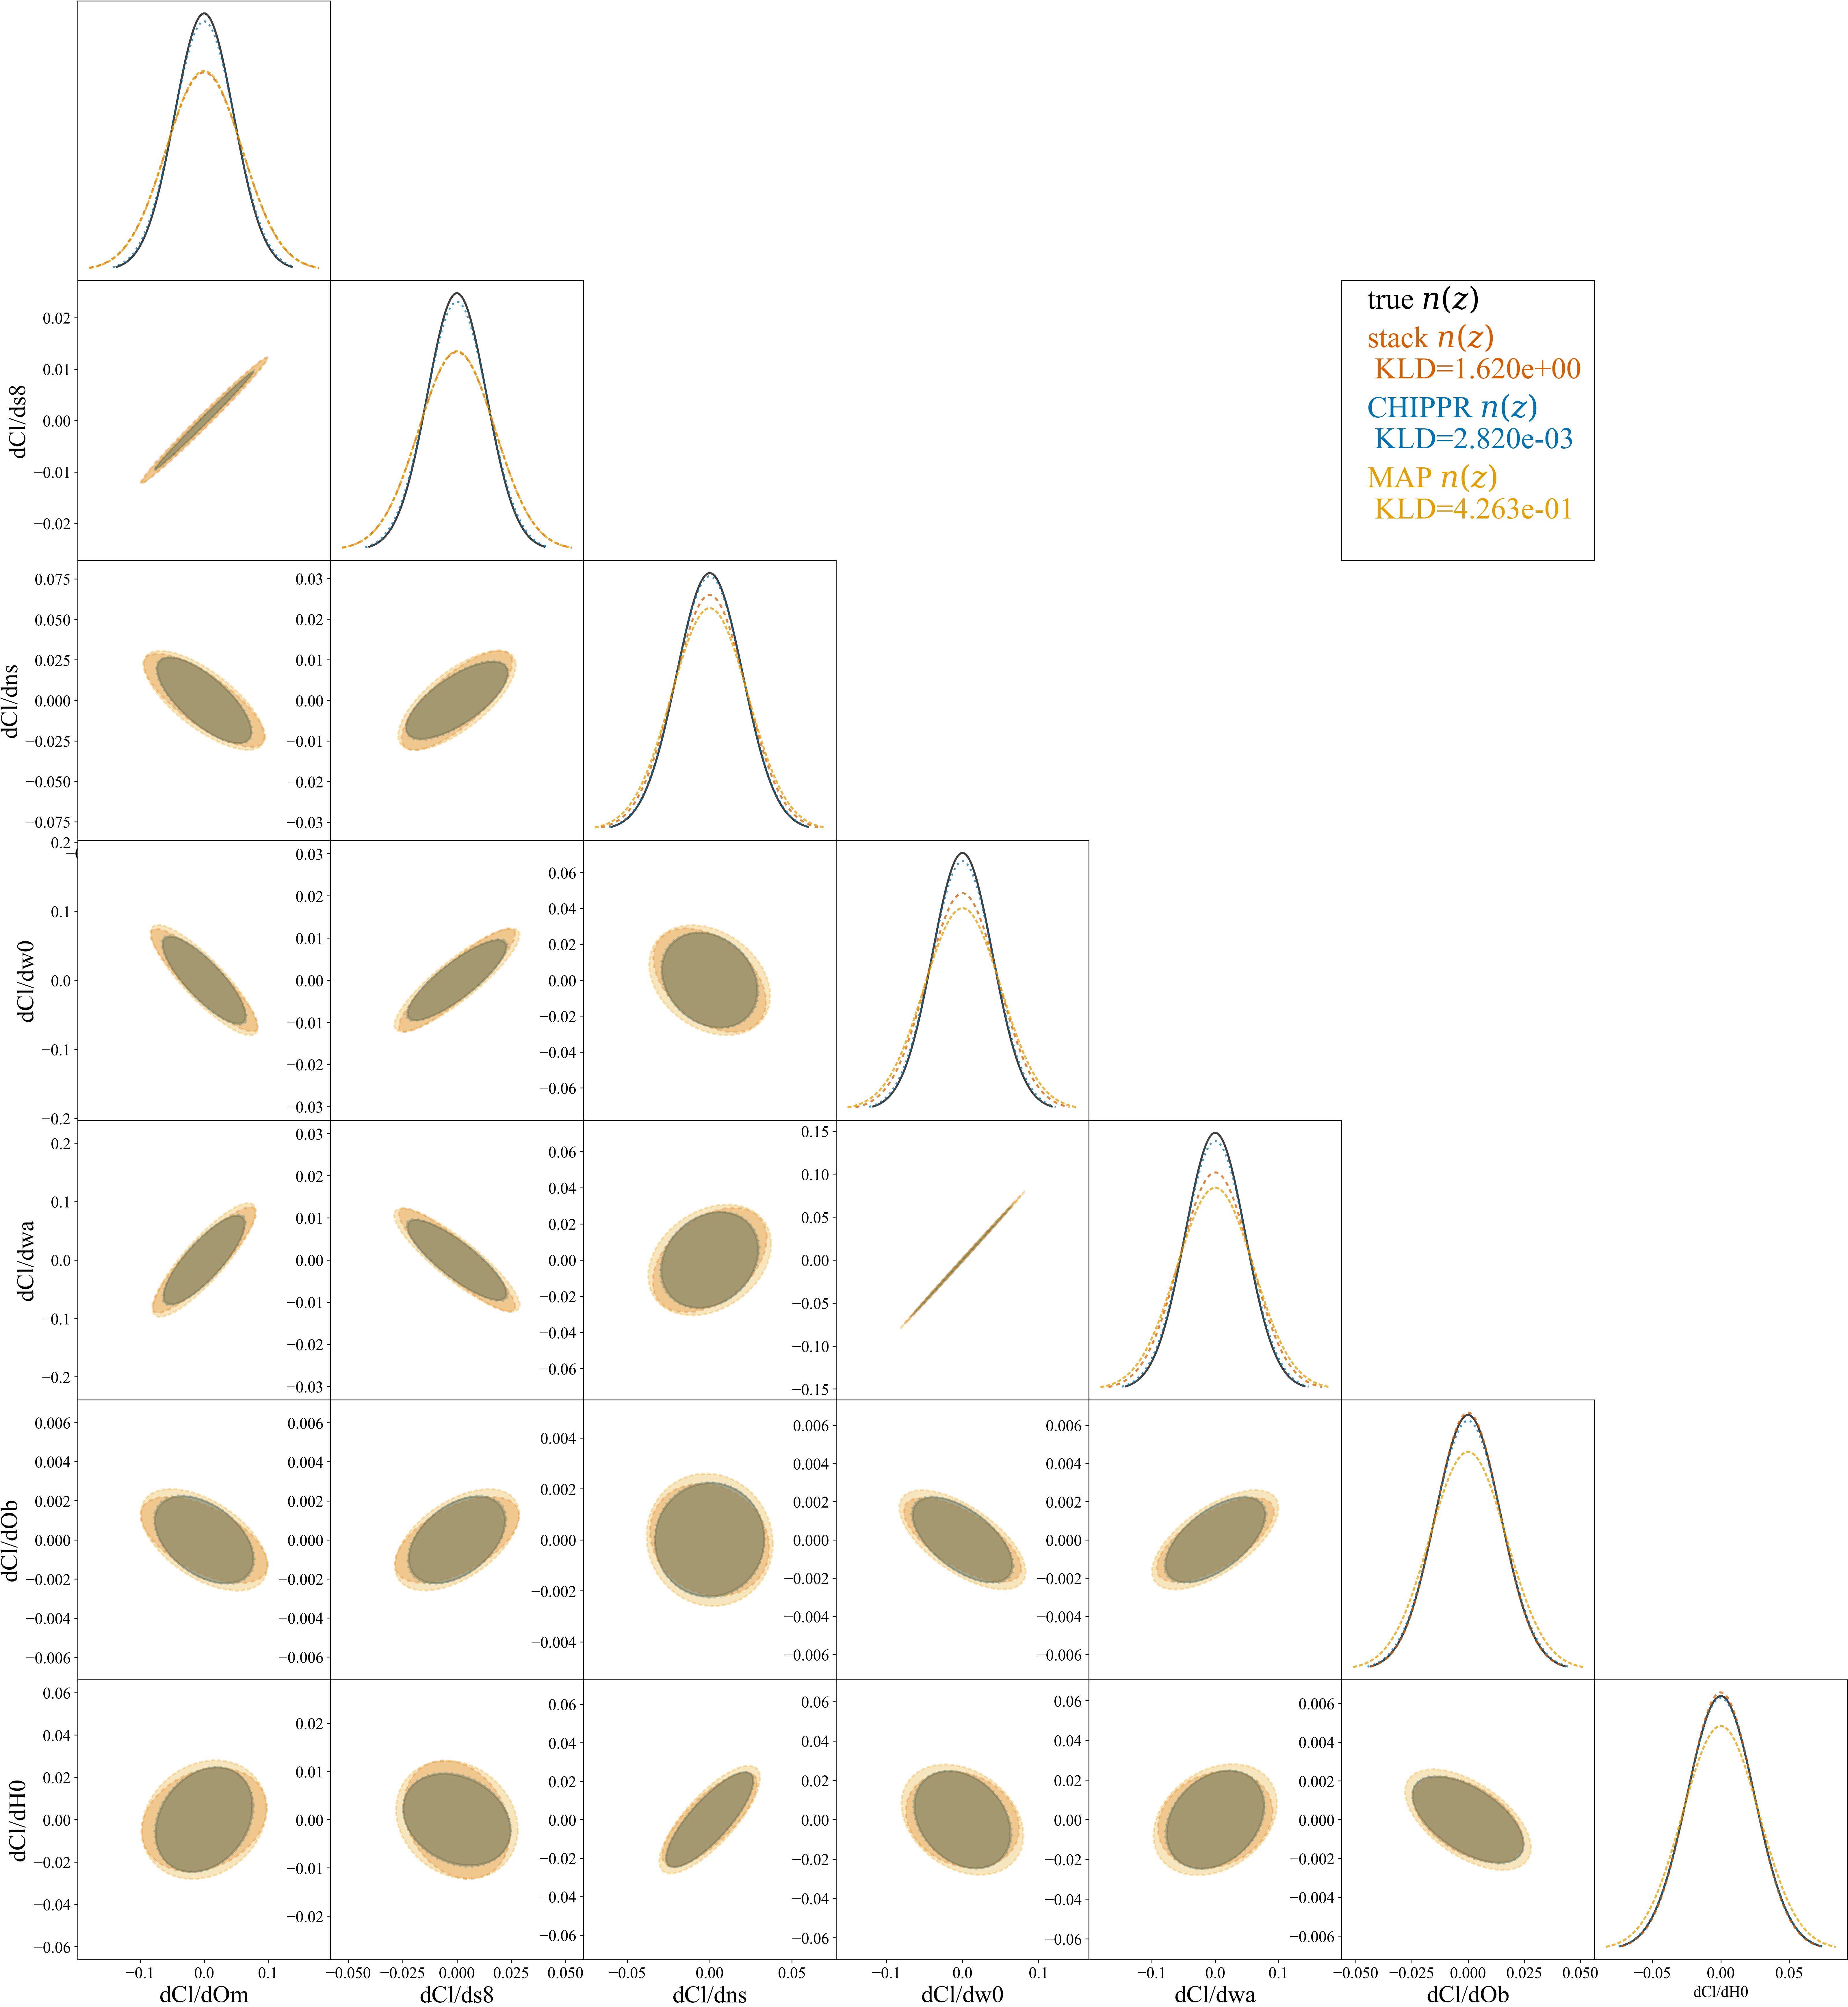
\includegraphics[width=0.99\textwidth]{figures/chippr/final_plot.png}
		\caption{The result of propagating the estimators of \nz\ of \Fig{fig:per-bin-ests} to a subset of cosmological parameters.}
		\figlabel{fig:cornerplot}
	\end{center}
\end{figure*}


\aim{Discuss these results here!}

\aim{Hogg says ``I think it would be good to talk a little quantitatively about where people need to know N(z) and other one-point statistics, and how much they will get various things wrong if they don't know these correctly. 
	And situate that discussion within the current context of cosmological parameter estimation and precision cosmology.''}

\aim{Caveats: I don't believe in tomographic binning because it's non-physical, and we won't have the true redshifts so there will be additional errors if tomography is used.}

\subsection{Violations of the model}
\sectlabel{sec:violations}

In these tests, the \pzip s are made to the \lsst\ requirements but the implicit prior used for the inference is not the same as the implicit prior used for generating the data.

\begin{figure*}
	\begin{center}
		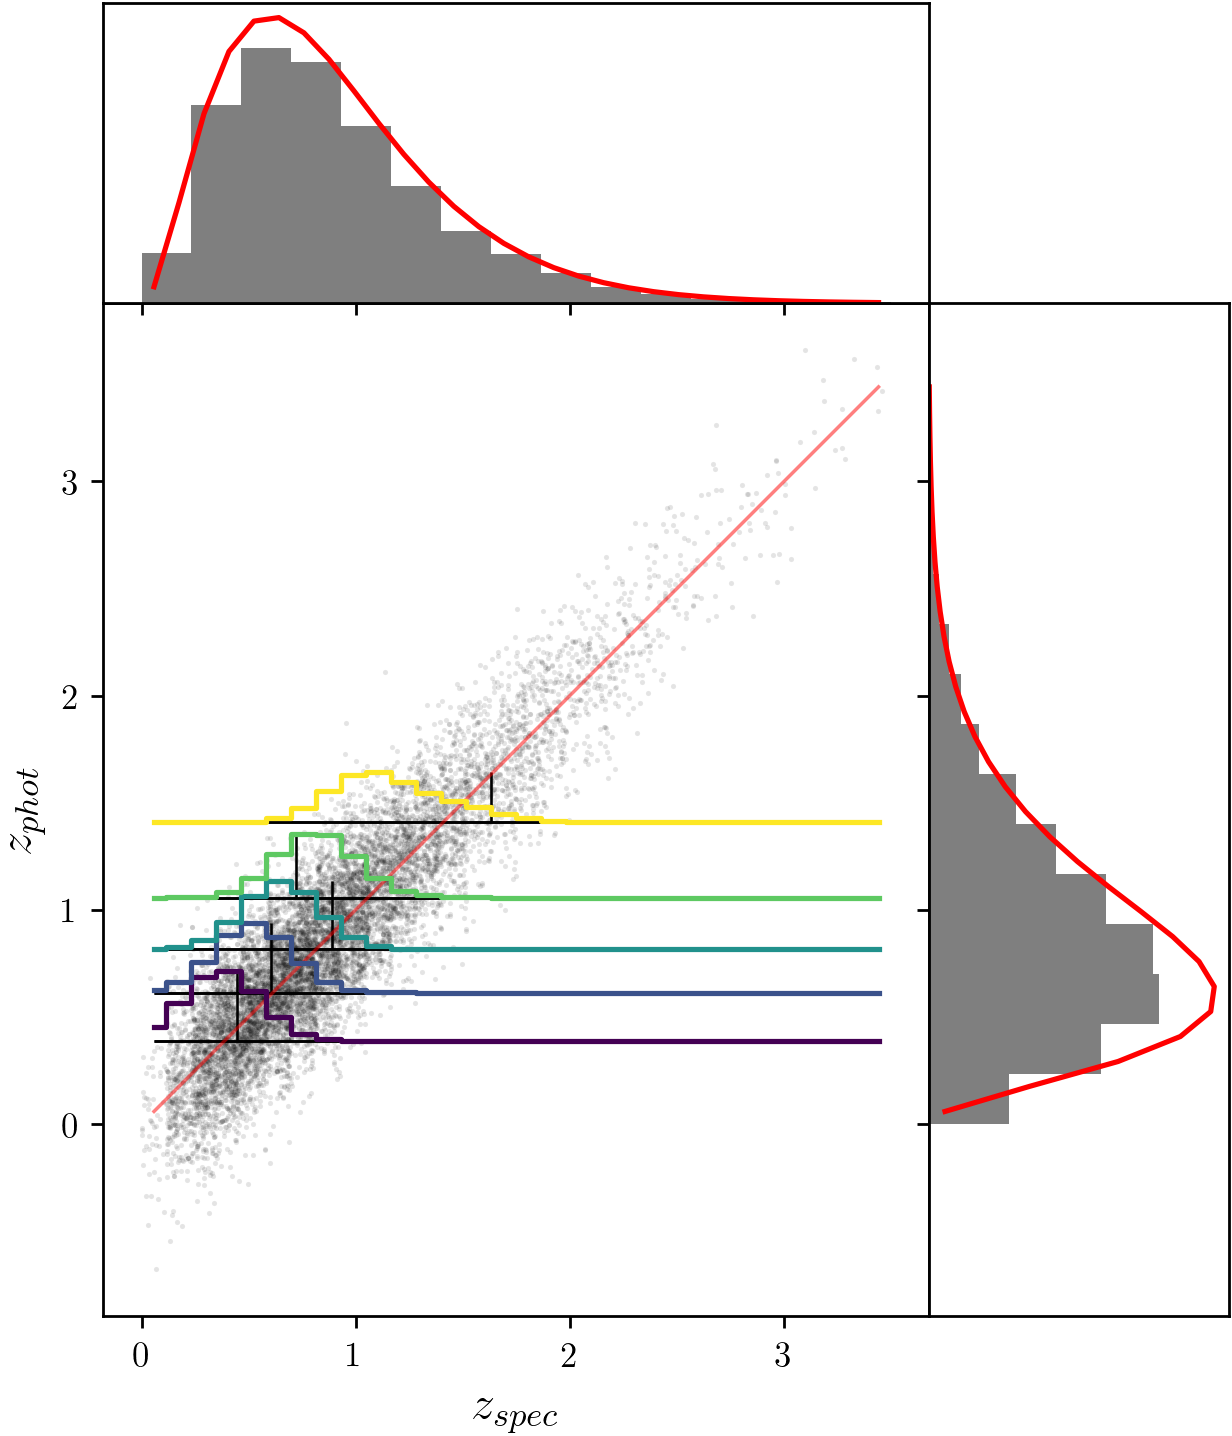
\includegraphics[width=0.45\textwidth]{figures/chippr/wrong_scatter.png}
		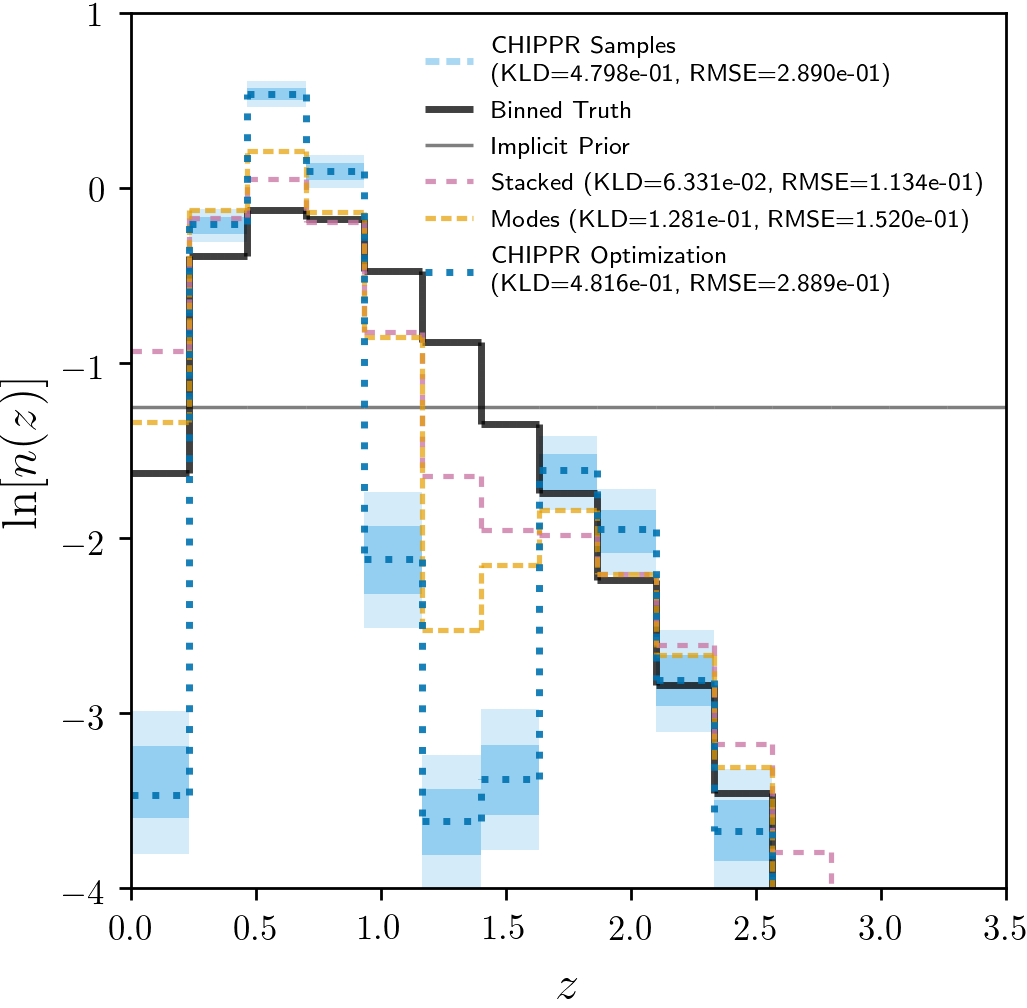
\includegraphics[width=0.45\textwidth]{figures/chippr/wrong_log_estimators.png}
		\caption{\aim{Update the figures for this to use the same conditions as \Sect{sec:lsstdemo} but one of the implicit priors from \Sect{sec:interim} for generating the data and the other for the inference.}}
		\figlabel{fig:mischaracterized}
	\end{center}
\end{figure*}

%\subsection{Real Data}
%\sectlabel{sec:boss}
%
%\aim{Commented out but may add back in later.}

%We also test this method on subsets of the published \pzpdf s of \sdss\ III DR 10. 
%A sampling of the provided interim photo-$z$ posteriors of dimension $K=35$ for $z_{min}=0.3$ and $z_{max}=1.4$ is shown in the top panel of \Fig{fig:datapzs}.  
%
%All tests in this paper will be conducted with $z_{0}=0.0$, $z_{K}=1.1$, and $K=35$, the endpoints and dimensionality of the published BOSS DR8 photo-$z$ interim posteriors \citet{Sheldon2012}.  
%We also define $\bar{z}_{k}\equiv(z_{k}+z_{k-1})/2$.
%The brightest half of this pseudo-random sampling are selected for another test, with photo-$z$ interim posterior samples shown in the bottom panel of \Fig{fig:datapzs}.  
%The interim prior used for this set of interim photo-$z$ posteriors is the reweighted estimator of $N(z)$ of \citet{Sheldon2012}.  
%In these cases the true $N(z)$ is not known, but the fully probabilistic method presented here may still be compared to what is obtained by alternative approaches.
%
%\begin{figure}
%	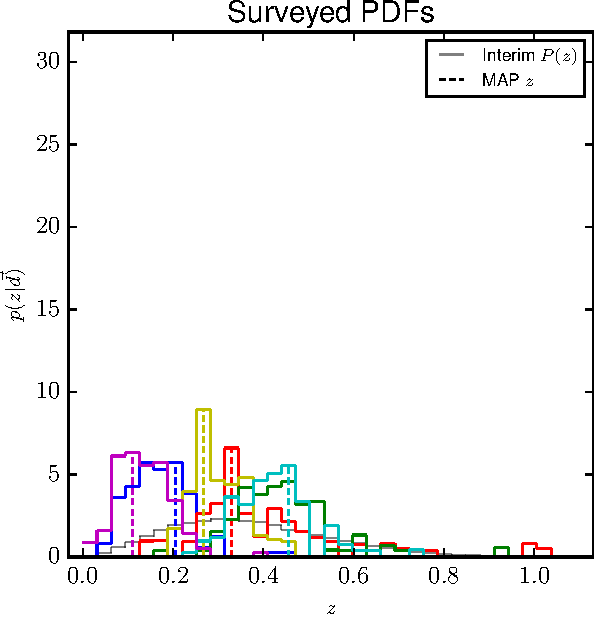
\includegraphics[width=0.5\textwidth]{figures/chippr/boss_samplepzs.pdf}\\
%	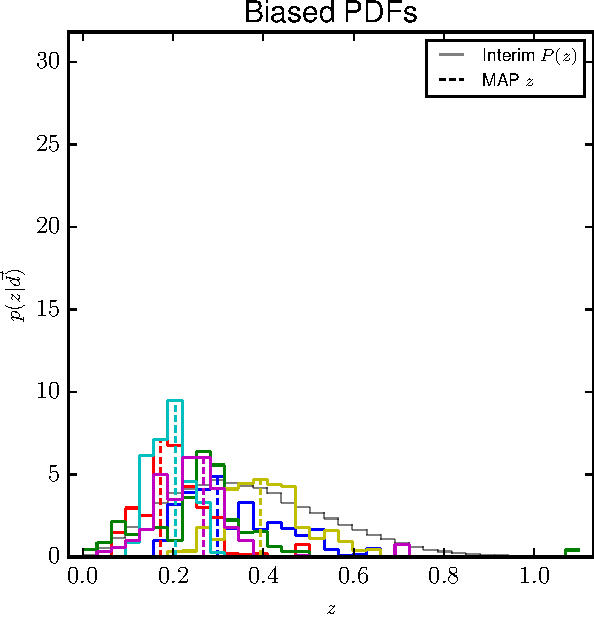
\includegraphics[width=0.5\textwidth]{figures/chippr/bias_samplepzs.pdf}
%	\caption{Same as \Fig{fig:nullpzs} but for real data.  
%		A pseudo-random sampling of BOSS DR 10 photo-$z$ posteriors produced by \citet{Sheldon2012} (top panel) are clearly much noisier than those of the fiducial case.  
%		A random sampling of the brightest half of the pseudo-random BOSS DR10 sample (bottom panel) corresponds to much cleaner photo-$z$ posteriors.}
%	\figlabel{fig:datapzs}
%\end{figure}

%The results of the inference of the redshift distribution function from a pseudo-random sample of BOSS DR10 data described in \Sect{sec:data} are shown in \Fig{fig:dataparam} and \Fig{fig:datacomp}.  
%
%The most striking feature of \Fig{fig:dataparam} aside from the stark difference between the mean of the samples and the interim prior is the major systematic in the samples from the posterior distribution is observed at high redshift.  
%Because the data itself exhibits high uncertainty at high $z$ in the form of local maxima of the photo-$z$ interim posteriors, a reflection of the inherent degeneracies that give rise to catastrophic photo-$z$ errors, it is natural that there be large errors in that region.  
%
%\begin{figure}
%	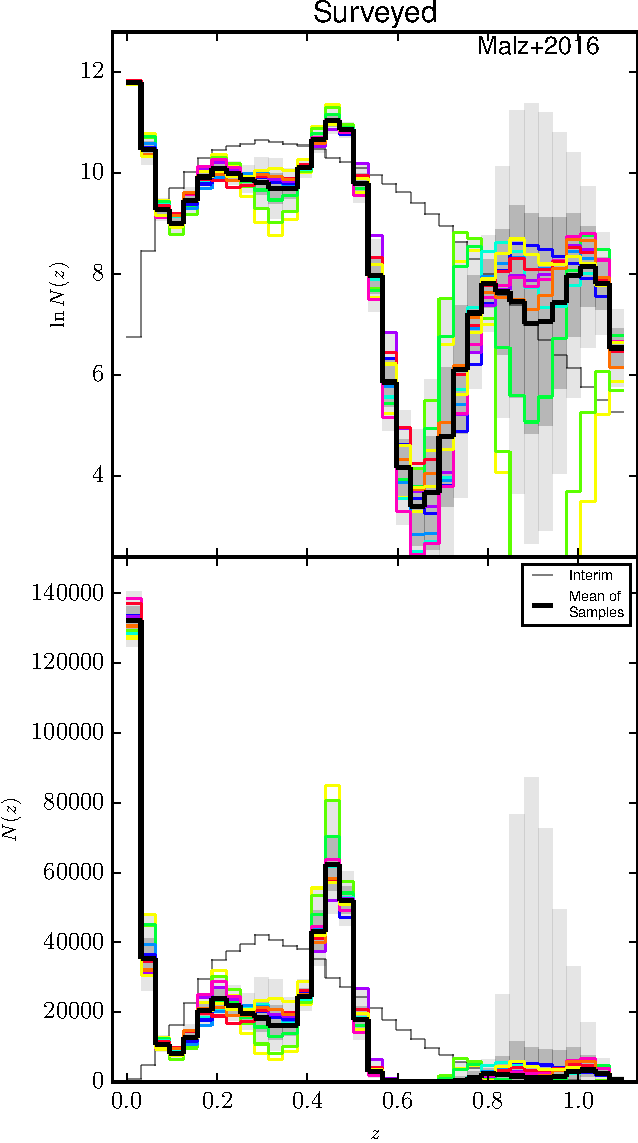
\includegraphics[width=0.5\textwidth]{figures/chippr/boss_samps.pdf}
%	\caption{Samples from the full posterior (colored lines) of the subsample differ substantially from the interim prior (gray).  
%		The mean of samples (thick, black line) and associated error bars ($1\sigma$ in dark gray, $2\sigma$ in light gray) are in line with the sampled values.}
%	\figlabel{fig:dataparam}
%\end{figure}
%
%\Fig{fig:datacomp} also shows the broader error bars in a small region of high redshift, but it has the additional information of how other estimators perform.  
%The results of stacking and reduction of interim photo-$z$ posteriors to point estimators are strongly biased toward the interim prior, especially stacking.  
%Given that stacking has been validated by the results' similarity to the interim prior, it is especially grave that it trivially reproduce it; if the interim prior is inappropriate, stacking is guaranteed to fail because it do not account for the effect of the interim prior on the interim photo-$z$ posteriors, permitting it to dominate over the underling likelihoods.  
%The result of marginalized maximum likelihood estimation is also shown to be numerically unstable, a possible effect of the extreme multimodality of the data.  
%
%\begin{figure}
%	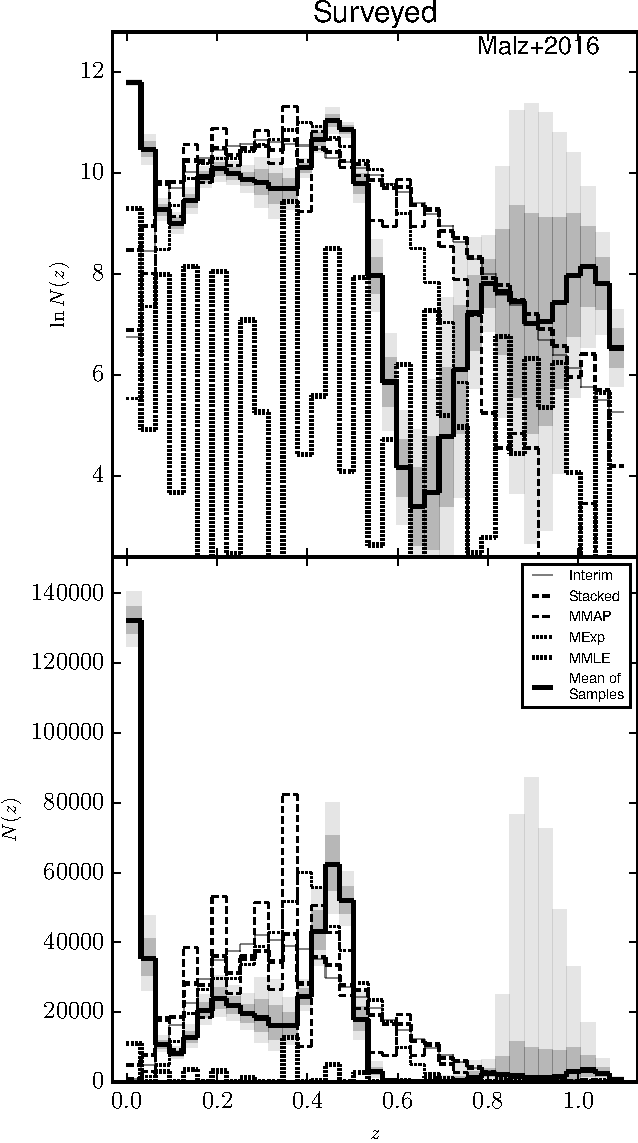
\includegraphics[width=0.5\textwidth]{figures/chippr/boss_comps.pdf}
%	\caption{It can be seen that the stacked estimator (thick, dashed line) almost perfectly reproduces the interim prior (gray line), while the marginalized maximum a posteriori estimator (thin, dashed line) and marginalized expected value estimator (thin, dotted line) do so with some instability.  
%		The marginalized maximum likelihood estimator (thick, dotted line) is most unstable, while the mean of the posterior samples (thick, solid line) predicts a very different redshift distribution function than the interim prior, with a peculiar feature in the error bars ($1\sigma$ in dark gray, $2\sigma$ in light gray) at high redshift.}
%	\figlabel{fig:datacomp}
%\end{figure}
%
%The BOSS subsample is further subsampled by imposing a cut in $r$-band magnitude (at the median magnitude) to approximate the behavior of a heavily biased galaxy survey with a magnitude limit.  
%This is motivated by the question of what data is behind the feature in the posterior distribution's error bars at high redshift.  
%Recall that samples of photo-$z$ interim posteriors are shown in the lower panel of \Fig{fig:datapzs}.  
%The results of the inference are shown in \Fig{fig:biasparam} and \Fig{fig:biascomp}.  
%
%\begin{figure}
%	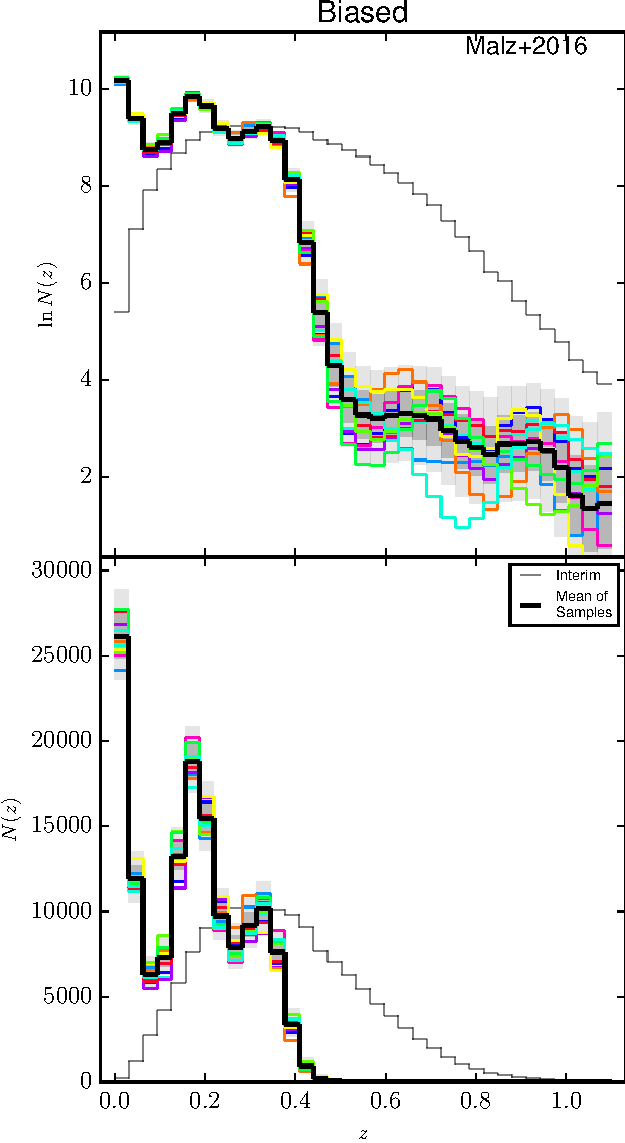
\includegraphics[width=0.5\textwidth]{figures/chippr/bias_samps.pdf}
%	\caption{Samples from the full posterior (colored lines) of the biased subsample still differ substantially from the interim prior (gray).  
%		The mean of samples (thick, black line) and associated error bars ($1\sigma$ in dark gray, $2\sigma$ in light gray) are in line with the sampled values.}
%	\figlabel{fig:biasparam}
%\end{figure}
%
%\begin{figure}
%	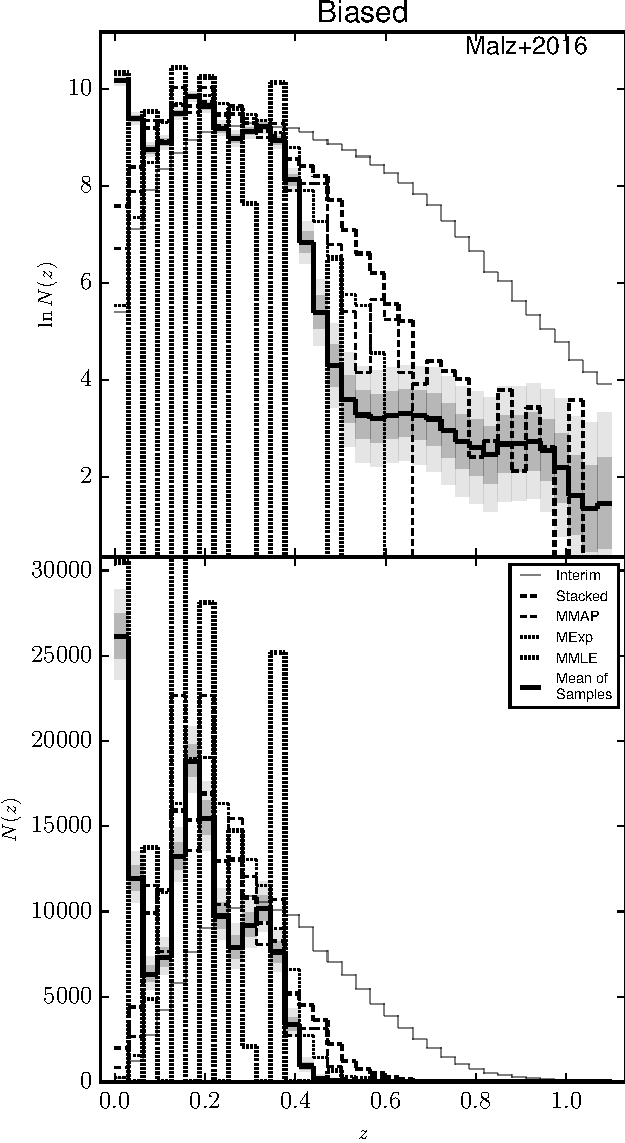
\includegraphics[width=0.5\textwidth]{figures/chippr/bias_comps.pdf}
%	\caption{The mean of posterior samples (thick, solid line) differs from the interim prior (gray line) more than the alternative estimators, exhibiting some features at low redshift.  
%		It can be seen that the stacked estimator (thick, dashed line) is most biased towards the interim prior, though the effect is also seen in the marginalized maximum a posteriori estimator (thin, dashed line) and marginalized expectation value estimator (thin, dotted line).  
%		The marginalized MLE (thick, dotted line) is still highly unstable.  
%		The error bars ($1\sigma$ in dark gray, $2\sigma$ in light gray) do not exhibit the same behavior as in the unbiased subsample.}
%	\figlabel{fig:biascomp}
%\end{figure}
%
%There are two notable differences between the unbiased and biased subsamples of the BOSS DR10 pseudo-random subsample.  
%First, the stacked and point estimators are less biased toward the interim prior.  
%This may be due to the way the interim prior was chosen, such that it was influenced strongly by the dimmest galaxies.  
%Second, the high-redshift feature in the error bars is not present once a magnitude cut is imposed.  
%From this one can conclude that the signal and associated error bars in that region were caused by the sampler's assignment high redshifts to poorly constrained interim photo-$z$ posteriors corresponding to the dimmest galaxies. 

\section{Conclusion}
\sectlabel{sec:con}

\aim{I still need to update the language in this section for consistency with the rest of \Chap{chippr}.}

This study derives and demonstrates a mathematically consistent implementation of inference of a one-point statistic based on implicit \pzpdf s.  
The fully Bayesian method, based in the fundamental laws of probability, begins with a graphical model corresponding to equations for the full posterior.  
The technique developed in this paper is applied to the example of the redshift density function \nz\ with promising results on mock data; not only is this the only mathematically correct approach to the problem, it also recovers the true parameter values better than popular alternatives.  

In the tests on simulated data performed here, the full posterior distribution over the hyperparameters defining $N(z)$ derived by this method is consistent with the true redshift distribution function, making the mean of sampled values an excellent point estimator of $N(z)$.  
The information contained in the full posterior distribution's shape convey the traditional error bar information without having to explicitly propagate any error estimates.  
\aim{Refer to quantitative results on KLD of \Nz\ and cosmological parameter space.}
%The results of those tests is summarized below and in \Tab{tab:kld}, where lower values indicate a closer match between the true $N(z)$ and the estimator.  
%Tests were also performed on subsets of BOSS DR10 data with results consistent with those of simulations.

The following conclusions and recommendations can be made with confidence:

\begin{enumerate}
	\item Both the marginalized maximum likelihood estimator and the mean of the samples are good point estimators of the redshift distribution function; the error bars on the posterior distribution over hyperparameters are generally reliable and easier to derive than error bars from traditional point estimators of the redshift distribution function.
	\item Even in the case of precise data, traditional methods fail, and they do even worse with imprecise data; the error bars of the mean of posterior samples, however, are accurate.  When data quality worsens with redshift, all estimators are affected, but the inaccuracy is quantified by the full distribution of the posterior samples whereas the alternative estimators require separate error propagation.  
	\item When data suffers from inaccuracies, as in the case of multimodal interim photo-$z$ posteriors, the marginalized maximum likelihood estimator performs comparably to the mean of the posterior samples
	\item The marginalized maximum likelihood estimator is an excellent estimator for strongly featured redshift distribution function with simple, clean photo-$z$ posteriors; stacking smooths features more than sampling and photo-$z$ point estimation.
	\item When the interim prior is known to be a poor approximation to the data, only the marginalized MLE and mean of sampled values are satisfactory estimators of the redshift distribution function because they are the only methods that can account for the bias introduced into the photo-$z$ posteriors; this is the most compelling case for the sampler because of the ubiquity of inappropriate interim priors.
\end{enumerate}

%\begin{table}
%	\begin{tabular}{lccccc}
%				& Mean of 		& Marginalized 	& Stacked 		& Marginalized 	& Marginalized\\
%				& Samples 		& MLE 			& Estimator 	& MAP 			& Expected Value\\
%	Fiducial 	&\textbf{0.0041}&0.0057			&0.0139			&0.0098			&0.0072\\
%	Precise 	&\textbf{0.0035}&0.0065			&0.0176			&0.0112			&0.0102\\
%	Imprecise 	&\textbf{0.0068}&0.0155			&0.1014			&0.1207			&0.1028\\
%	Trending 	&\textbf{0.0199}&0.0262			&0.1057			&0.1288			&0.0813\\
%	Multimodal 	&\textbf{0.0052}&0.0054			&0.0508			&0.0385			&0.0250\\
%	Sampled 	&0.0189			&\textbf{0.0026}&0.0475			&0.0446			&0.0230\\
%	Featured 	&0.0104			&\textbf{0.0060}&0.2902			&0.1721			&0.1720\\
%	Unimodal 	&\textbf{0.0030}&0.0046			&0.0150			&0.0128			&0.0127\\
%	Bimodal 	&\textbf{0.0037}&0.0056			&0.0143			&0.0122			&0.0141
%	\end{tabular}
%	\caption{The KLD values for all estimators in each simulated test are provided here.
%		The best-fit estimator in each case is bolded.}
%	\tablabel{tab:kld}
%\end{table}

By showing that this method is effective in recovering the true redshift distribution function and posterior distributions on its parameters from catalogs of \pzpdf s, this work supports the production of \pzpdf s by upcoming photometric surveys such as \lsst\ so that more accurate inference of physical parameters may be accessible to the scientific community.  
We discourage researchers from co-adding \pzpdf s or converting them into point estimates of redshift and instead recommend the use of Bayesian probability to guide the usage of \pzpdf s in science.  
We emphasize to those who produce \pzpdf s from data that it is essential to release the implicit prior used in generating this data product in order for proper inference to be conducted by consumers of this information.

The technique herein developed is applicable with minimal modification to other one-point statistics of redshift to which we will apply this method in the future, such as the redshift-dependent luminosity function and weak lensing mean distance ratio.  
Future work will also include the extension of this fully probabilistic approach to higher-order statistics of redshift such as the two-point correlation function.

\aim{What else should I be putting here?  
	Is this a good place to put the discussion of how different estimators of \Nz\ affect different estimators of the weak lensing power spectrum?  
	That analysis is currently in \Sect{sec:lsstdemo}.}

\section*{Chapter acknowledgements}

I thank Elisabeth Krause for assistance with the \texttt{CosmoLike} code, Mohammadjavad Vakili for statistical insights, Geoffrey Ryan for programming advice, and Boris Leistedt for other helpful comments in the development of \Chippr.

\renewcommand{\chapid}{pzdc1}

% Chapter specific commands:

% Math:

% projects
\newcommand{\kids}{\project{KiDS}}
\newcommand{\hsc}{\project{HSC}}
\newcommand{\wfirst}{\project{WFIRST}}
\newcommand{\buzz}{\project{Buzzard}}
\newcommand{\pzwg}{\textit{PZWG}}

% can easily change these to specify posterior throughout, etc
\newcommand{\chisq}{$\chi^{2}$}

% codes
\newcommand{\annz}{\pzcode{ANNz2}}
\newcommand{\bpz}{\pzcode{BPz}}
\newcommand{\cmnn}{\pzcode{CMNN}}
\newcommand{\delight}{\pzcode{Delight}}
\newcommand{\eazy}{\pzcode{EAZY}}
\newcommand{\flexzboost}{\pzcode{FlexZBoost}}
\newcommand{\gpz}{\pzcode{GPz}}
\newcommand{\lephare}{\pzcode{LePhare}}
\newcommand{\metaphor}{\pzcode{METAPhoR}}
\newcommand{\skynet}{\pzcode{SkyNet}}
\newcommand{\tpz}{\pzcode{TPZ}}
\def\X{{\mathbf{X}}}
\def\x{{\mathbf{x}}}
\def\E{{\mathbb{E}}}

\chapter{ Evaluation of probabilistic photometric redshift estimation approaches \chaplabel{pzdc1} }

This \paper\ represents joint work with Sam Schmidt (UC Davis) and the entire Photo-Z Working Group (\pzwg) of the \desc, which is intended for submission to MNRAS and whose public draft\footnote{\url{{https://github.com/LSSTDESC/PZDC1paper}}} is currently in \desc\ internal review.
The words of the paper were written by the entire \pzwg\ over the course of three years, though the bulk of the writing was executed by myself, Sam Schmidt (UC Davis), and John Soo (U. of Science Malaysia).
The detailed contributions of over twenty co-authors are provided at the end of this \paper\ but I describe the work for which I was responsible and acknowledge those who helped directly with those aspects of the \paper\ here.

My role was to choose, implement, and interpret the metrics by which the \pzpdf\ codes would be evaluated, an important aspect of experimental design that had not been addressed already.
I chose the metrics with input from Jeff Newman (Pitt) and Ann Lee (CMU), as well as discussions with the entire \pzwg\ from late 2016 through early 2018.
In summer and fall 2017, I implemented the metrics in code and ran them on the results of the \pzpdf\ codes with the assistance of Rongpu Zhou (Pitt), Bryce Kalmbach (UW), Kartheik Iyer (Rutgers), Sam Schmidt (UC Davis), and Chris Morrison (UW).
The interpretation of the metrics, culminating in both of the major discoveries of the paper, those of the isolation of the implicit prior and the flaws of traditional metrics, was mine alone, though the presentation of these points benefited from input from Sam Schmidt (UC Davis) and Chris Morrison (UW) througout 2018.
I devised and implemented \trainz\ in the process of choosing and interpreting the metrics as a demonstration of the limitations of all metrics previously used for \pzpdf s.

%\aim{Change the British spelling back to American for thesis.}

\section*{Chapter abstract}

Many scientific investigations of photometric galaxy surveys require redshift estimates, whose uncertainty properties are best encapsulated by photometric redshift (photo-$z$) posterior probability distribution functions (PDFs).
A plethora of photo-$z$ PDF estimation methodologies abound, producing discrepant results with no consensus on a preferred approach.
We present the results of a comprehensive experiment comparing twelve photo-$z$ algorithms on mock data produced for the Large Synoptic Survey Telescope (\textsc{LSST}) Dark Energy Science Collaboration (\textsc{DESC}).
By supplying perfect prior information, in the form of the complete template library and a representative training set as inputs to each code, we demonstrate the impact of the assumptions underlying each technique on the output photo-$z$ PDFs.
In the absence of a notion of true, unbiased photo-$z$ PDFs, we evaluate and interpret multiple metrics of the ensemble properties of the derived photo-$z$ PDFs as well as traditional reductions to photo-$z$ point estimates.
We report systematic biases and overall over/under-breadth of the photo-$z$ PDFs of many popular codes, which may indicate avenues for improvement in the algorithms or implementations.
Furthermore, we raise attention to the limitations of established metrics for assessing photo-$z$ PDF accuracy; though we identify the conditional density estimate (CDE) loss as a promising metric of photo-$z$ PDF performance in the case where true redshifts are available but true photo-$z$ PDFs are not, we emphasize the need for science-specific performance metrics.

\section{Introduction}

The current and next generations of large-scale galaxy surveys, including the Dark Energy Survey \citep[\des,][]{Abbott:05}, the Kilo-Degree Survey \citep[\kids,][]{de_Jong:13}, Hyper Suprime-Cam Survey \citep[\hsc,][]{Aihara:2018a,Aihara:2018b}, Large Synoptic Survey Telescope \citep[\lsst,][]{Abell:09}, Euclid \citep{Laureijs:11}, and Wide-Field Infrared Survey Telescope \citep[\wfirst,][]{Green:12}, present a paradigm shift from spectroscopic to photometric galaxy catalogues of substantially larger size at a cost of lacking complete spectroscopically confirmed redshifts ($z$).

Effective astrophysical inference using the catalogues resulting from these ongoing and upcoming missions, however, necessitates accurate and precise photometric redshift (\pz) estimation methodologies.
As an example, in order for \pz\ systematics to not dominate the statistical noise floor of \lsst's main cosmological sample of $\sim 10^{7}$ galaxies, the \lsst\ Science Requirements Document (SRD)\footnote{available at \url{https://docushare.lsstcorp.org/docushare/dsweb/Get/LPM-17}} specifies that individual galaxy \pz s must have root-mean-square error $\sigma_z < 0.02 (1+z)$, $3 \sigma$ catastrophic outlier rate below $10\%$, and bias below $0.003$.
Specific science cases may have their own requirements on \pz\ performance that exceed those of the survey as a whole.
In that vein, the \lsst\ Dark Energy Science Collaboration (\desc) developed a separate SRD \citep{Mandelbaum:2018} that conservatively forecasts the constraining power of five cosmological probes, leading to even more stringent requirements on \pz\ performance, including those defined in terms of tomographically binned subsamples populations rather than individual galaxies.

% MOVE TO WHERE \nz\ IS INTRODUCED AS A METRIC
% For cosmological measurements, certain science cases require redshift information on individual objects, e.~g.~identification of host galaxy redshift for supernova classification, or identifying potential cluster membership.
% Other science cases seem to need only ensemble redshift information; for instance many current cosmic shear techniques require only the overall redshift distribution $N(z)$ for tomographic redshift samples.
% However,  even such cases require individual object redshift estimates for portions of the analysis, for example in determining galaxy intrinsic alignments in weak lensing samples.
% In addition, recent data-driven techniques employing hierarchical Bayesian or Gaussian Process methods have emerged that calibrate redshift distributions using individual $p(z)$ estimates \citep[e.~g.~][]{Sanchez:2018}.
% Techniques for using \pzpdf s have lagged behind the development of codes to produce them, however, all existing approaches assume that the \pzpdf\ for each galaxy is an accurate PDF, with failures when the assumption is violated.
% Thus, even methods that seem to need only ensemble $N(z)$ may actually require accurate $p(z)$ in order to meet stringent survey requirements.
% Large photometric surveys such as LSST must develop algorithms that simultaneously meet the needs of all science cases.
% In order to meet these ambitious goals for photo-$z$ accuracy, every aspect of photo-$z$ estimation will have to be optimized: the algorithms employed, both template and machine-learning based (both in design and implementation); the spectroscopic data used as a training set for machine learning algorithms or to estimate template sets and train Bayesian priors; and probabilistic catalogue compression schemes that balance information retention against limited storage resources.

Though the standard has long been for each galaxy in a photometric catalogue to have a \pz\ point estimate and Gaussian error bar, the nontrivial mapping between broad band fluxes and redshift renders this simplistic summary inadequate to quantify the uncertainty landscape by neglecting degenerate redshift solutions.
Far from a hypothetical situation, this degeneracy is a real consequence of the same deep imaging that enables larger galaxy catalogue sizes.
The lower luminosity and higher redshift populations captured by deeper imaging introduce major physical systematics to \pz s, among them the Lyman break/Balmer break degeneracy, that did not affect shallower large area surveys like the Sloan Digital Sky Survey \citep[\textsc{SDSS},][]{York:00} and Two Micron All Sky Survey \citep[\textsc{2MASS},][]{Skrutskie:06}.

To fully characterize such physical degeneracies, photometric galaxy catalogue data releases from \citep{mandelbaum_precision_2008} to \citep{de_Jong:17}, provided a more informative \pz\ data product, the \pz\ probability density function (PDF), that describes the redshift probability, commonly denoted as $p(z)$, as a function of a galaxy's redshift, conditioned on the observed photometry.
Early template-based methods such as \citet{Fernandezsoto:99} approximated the likelihood of photometry conditioned on redshift with the relative \chisq\ values of template spectra.
Not long after, Bayesian adaptations of template-based approaches such as \citet{benitez_bayesian_2000} combined the estimated likelihoods with a prior to yield a posterior PDF of redshift conditioned on photometry.
While the first data-driven \pz\ algorithms yielded a point estimate, \citet{Firth:03} estimated a \pzpdf\ using a neural net with realizations scattered within the photometric errors.

There are numerous techniques for deriving \pzpdf s, yet no one method has yet been established as clearly superior.
Quantitative comparisons of \pz\ methods have been made before.
The \Pz\ Accuracy And Testing \citep[\textsc{PHAT},][]{Hildebrandt:10} effort focused on \pz\ point estimates derived from many photometric bands.
\citet{Rau:2015} introduced a new method for improving \pzpdf s using an ordinal classification algorithm.
\textsc{DES} compared several codes for \pz\ point estimates and a subset with \pzpdf\ information \citep{Sanchez:14} and examined summary statistics of \pzpdf s for tomographically binned galaxy subsamples \citep{bonnett_redshift_2016}.

This paper is distinguished by its focus on the evaluation criteria for \pzpdf s and interpretation thereof, as a key project of the Photometric Redshifts working group of the \desc\ that aims to perform a comprehensive sensitivity analysis of \pzpdf\ techniques in order to ultimately select those that will become part of the \lsst\ pipelines, as laid out in the Science Road Map (SRM)\footnote{Available at: \url{http://lsst-desc.org/sites/default/files/DESC_SRM_V1_1.pdf}\label{lsstdesc_srm}}.
In this initial study, we focus on evaluating the performance of \pzpdf\ codes using PDF-specific performance metrics in a controlled experiment with complete and representative prior information (template libraries and training sets) to set a baseline for subsequent investigations.
This approach probes how each code considered exploits the information content of the data versus prior information from template libraries and training sets.

The outline of the paper is as follows: in \Sect{sec:sims} we present the simulated data set; in \Sect{sec:pzcodes} we describe the current generation codes employed in the paper; in \Sect{sec:metrics} we discuss the interpretation of photo-$z$ PDFs in terms of metrics of accuracy; in \Sect{sec:results} we show our results and compare the performance of the codes; in \Sect{sec:discussion} we offer our conclusions and discuss future extensions of this work.

\section{Data}
\sectlabel{sec:sims}

In order to test the current generation of \pzpdf\ codes, we employ an existing simulated galaxy catalogue, described in detail in \Sect{sec:buzzard}.
The experimental conditions shared among all codes are motivated by the \lsst\ SRD requirements and implemented for machine learning and template-based \pzpdf\ codes according to the procedures of \Sect{sec:buzztraining} and \Sect{sec:buzztemplates} respectively.

\subsection{The \textsc{Buzzard-v1.0} simulation}
\sectlabel{sec:buzzard}

Our mock catalogue is derived from the \textsc{Buzzard}-highres-v1.0  of De Rose et al., in prep, Wechsler et al., in prep) catalogue.
% UPDATE THIS CITATION NOW THAT THE PAPER IS OUT
\textsc{Buzzard} is built on a dark matter-only N-body simulation of $2048^{3}$ particles in a $400$ Mpc h$^{-1}$ box.
The lightcone was constructed from smoothing and interpolation between a set of time snapshots.
Dark matter halos were identified using the \texttt{Rockstar} software package \citep{Behroozi:13} and then populated with galaxies with a stellar mass and absolute $r$-band magnitude in the \sdss\ system determined using a sub-halo abundance matching model constrained to match both projected two-point galaxy clustering statistics and an observed conditional stellar mass function \citep{Reddick:13}.

To assign a spectrum to each galaxy, the Adding Density Dependent Spectral Energy Distributions (SEDs) procedure (\texttt{ADDSEDS}, deRose in prep.)\footnote{\url{https://github.com/vipasu/addseds}} was used.
\texttt{ADDSEDS} uses a sample of $\sim 5\times 10^{5}$ galaxies from the magnitude-limited \sdss\ Data Release 6 Value Added Galaxy Catalogue \citep{Blanton:05} to train an empirical relation between absolute $r$-band magnitude, local galaxy density, and SED.
Each \sdss\ spectrum is parameterized by five weights corresponding to a weighted sum of five basis SED components using the \texttt{k-correct v4\_3} software package\footnote{\url{http://kcorrect.org}} \citep{Blanton:07}.

Correlations between SED and galaxy environment were included so as to preserve the colour-density relation of galaxy environment.
The distance to the spatially projected fifth-nearest neighbour was used as a proxy for local density in the \sdss\ training sample.
For each simulated galaxy, a galaxy with similar absolute $r$-band magnitude and local galaxy density was chosen from the training set, and that training galaxy's SED was assigned to the simulated galaxy.
In \Sect{sec:buzzlimitations}, we critique the realism of this mock data.

\subsubsection{Caveats}
\sectlabel{sec:buzzlimitations}

By necessity, \textsc{Buzzard} does not contain all of the complicating factors present in real data, and here we discuss the most pertinent ways that this limitation affects our experiment.
% In several cases, the simplification is done with a purpose, with potentially confounding effects excluded in order to better isolate the differences between current-generation photo-$z$ codes and their causes.
\textsc{Buzzard} includes only galaxies, not stars of AGN.
The catalogue-based construction excludes image-level effects, such as deblending errors, photometric measurement issues, contamination from sky background (Zodiacal light, scattered light, etc.), lensing magnification, and Galactic reddening.

The SEDs are five-component linear combinations of $\sim 5 \times 10^{5}$ \sdss\ galaxies, so the sample contains only galaxies that resemble linear combinations of those for which \sdss\ obtained spectra.
The linear combination SEDs also restrict the properties of the galaxy population to linear combinations of the properties corresponding to five basis templates, precluding the modeling of non-linear features such as the full range of emission line fluxes relative to the continuum.
The only form of intrinsic dust reddening comes from what is already present in the five basis SEDs via the training set used to create the basis templates, and linear combinations thereof do not span the full range of realistic dust extinction observed in galaxy populations.

While these idealized conditions limit the realism of our mock data, they are irrelevant to the controlled experimental conditions of this study, if anything assuring that differentiation in the performance of the \pzpdf\ codes is due to the inferential techniques rather than nuances in the data.

\subsection{\lsst-like mock observations}
\sectlabel{sec:observations}

Given the SED, absolute $r$-band magnitude, and redshift, we computed apparent magnitudes in the six \lsst\ filter passbands, $ugrizy$.
We assigned magnitude errors in the six bands using the simple model of \citet{Ivezic:08}, assuming achievement of the full 10-year depth, with a modification of fiducial \lsst\ total numbers of 30-second visits for photometric error generation: we assume 60 visits in $u$-band, 80 visits in $g$-band, 180 visits in $r$-band, 180 visits in $i$-band, 160 visits in $z$-band, and 160 visits in $y$-band.
%numbers taken from Alex Abate's photErrorModel.py script in PhotoZDC1 repository, which was used with nYrObs=10.

As a consequence of adding Gaussian-distributed photometric errors, 2.0\% of our galaxies exhibit a negative flux in one or more bands, the vast majority of which are in the $u$-band.
We deem such negative fluxes \textit{non-detections} and assign a placholder magnitude of 99.0 in the catalogue to indicate to the \pzpdf\ codes that such galaxies would be ``looked at but not seen'' in multi-band forced photometry.

The full dataset thus covers $400$ square degrees and contains $238$ million galaxies of redshift $0 < z \leq 8.7$ down to $r = 29$.
Systematic inconsistencies with galaxy colors at $z > 2$ were observed, so the catalogue was limited to $0 < z \leq 2.0$.
To obtain a catalogue matching the \lsst\ Gold Sample, we imposed an cut of $i < 25.3$, which gives a signal-to-noise ratio $\sim 30$ for most galaxies.
In order for statistical errors to be subdominant to the systematic errors we aim to probe, we further reduced the sample size to $<10^{7}$ galaxies by isolating $\sim 16.8$ square degrees selected from five separate spatial regions of the simulation.
We refer to this final set of galaxies as DC1, for the first \desc\ Data Challenge.

\subsection{Shared prior information}
\sectlabel{sec:controlled}

% NOW MOTIVATE THE SHARED PRIOR INFORMATION
For the purpose of performing a controlled experiment that compares \pzpdf\ codes on equal footing as a baseline for a future sensitivity analysis, we take care to provide each with maximally optimistic prior information.
Redshift estimation approaches built upon physical modeling and machine learning alike have a notion of prior information considered beyond the photometry of the data for which redshift is to be constrained: that information is derived from a template library for a model-based code and a training set for a data-driven code.
In this initial study, we seek to set a baseline for a later comparison of the performance of \pzpdf\ codes under incomplete and non-representative prior information that will propagate differently in the space of data-driven and model-based algorithms.
However, for the baseline case of perfect prior information, physical modeling and machine learning codes can indeed be put on truly equal footing.
We outline the equivalent ways of providing all codes perfect prior information below.

\subsubsection{Training and test set division}
\sectlabel{sec:buzztraining}

Following the findings of \citet{Bernstein:10}, \citet{Masters:2017} that only $~10^{4}$ spectra are necessary to calibrate \pz s to Stage IV requirements, we aimed to set aside a randomly selected training set of $3-5\times 10^{4}$ galaxies, $\sim 10\%$ of the full sample.
After all cuts described above, we designated the \textit{DC1 training set} of $44\,404$ galaxies for which observed photometry, true SEDs, and true redshifts would be provided to all codes codes and the blinded \textit{DC1 test set} of $399\,356$ galaxies for which photometry alone would be provided to all codes and \pzpdf s would be requested.
%The resulting catalogues contain $111\,171$ training galaxies and $1\,000\,883$ test galaxies.
The \lsst\ photometric filter transmission curves were also considered public information that could be used by any code.

\subsubsection{Template library construction}
\sectlabel{sec:buzztemplates}

We aimed to provide template-fitting codes with complete yet manageable library of templates spanning the space of SEDs of the DC1 galaxies.
We constructed $K=100$ representative templates from the $\sim 5 \times 10^{5}$ SEDs of the \sdss\ DR6 NYU-VAGC by using the five-dimensional vectors of SED weight coefficients described above.
After regularizing the SED weight coefficients $\in [0, 1]$, we ran a simple K-means clustering algorithm on the five-dimensional space of regularized SED weight coefficients of the \sdss\ galaxy sample.
The resulting clusters were used to define Voronoi cells in the space of weight coefficients, with centre positions corresponding to weights for the \texttt{k-correct} SED components, yielding the 100 \textit{DC1 template set} to be provided to all template-based codes.
We did not, however, exclude from consideration template-based codes that made modifications in their use of these templates due to architecture limitations (as opposed to knowledge of the experimental conditions that could artificially boost the code's apparent performance), with deviations noted in \Sect/{sec:pzcodes}.

\section{Methods}
\sectlabel{sec:pzcodes}

Here we summarize the twelve \pzpdf\ codes compared in this study, summarized in \Tab{tab:list_of_codes}, which include both established and emerging approaches in template fitting and machine learning.
Though not exhaustive, this sample represents codes for which there was sufficient expertise within the \desc\ Photometric Redshifts Working Group; the authors welcome interest from those outside \desc\ to have their codes assessed in future investigations that build upon this one.

\begin{table*}  %%% DATA TABLE %%%
	\caption{List of \pzpdf\ codes featured in this study} \tablabel{tab:list_of_codes}\resizebox{\textwidth}{!}{
		\begin{tabular}{lll}
			\hline
			\bf Published code & \bf Type & \bf Public source code \\
			\hline
			\lephare~\citep{Arnouts:99}	   & template fitting	& \url{http://www.cfht.hawaii.edu/~arnouts/lephare.html} \\
			\bpz~\citep{benitez_bayesian_2000} 		   & template fitting	& \url{http://www.stsci.edu/~dcoe/BPZ/} \\
			\eazy~\citep{Brammer:08}		   & template fitting & \url{https://github.com/gbrammer/eazy-photoz} \\
			\annz~\citep{sadeh_annz2:_2016}		     & machine learning	& \url{https://github.com/IftachSadeh/ANNZ} \\
			\flexzboost~\citep{Izbicki:17} & machine learning & \url{https://github.com/tpospisi/flexcode}; \url{https://github.com/rizbicki/FlexCoDE}\\
			%\textsc{Frankenz} 	& ML 	& \citet{Speagle:frankenz}	& \url{https://github.com/joshspeagle/frankenz} \\
			\gpz~\citep{Almosallam:15b}	   & machine learning	& \url{https://github.com/OxfordML/GPz} \\
			\metaphor~\citep{Cavuoti:17}   & machine learning	& \url{http://dame.dsf.unina.it}\\
			\cmnn~\citep{Graham:17}        & machine learning & N/A \\
			\skynet~\citep{Graff:14}       & machine learning & \url{http://ccpforge.cse.rl.ac.uk/gf/project/skynet/} \\
			\tpz~\citep{Carrasco_Kind:13}	 & machine learning	& \url{https://github.com/mgckind/MLZ} \\
			\delight~\citep{Leistedt:17}   & hybrid           & \url{https://github.com/ixkael/Delight} \\
			\hline
			\trainz 	                             & machine learning	& See \Sect{sec:trainz} \\
	\end{tabular}}
\end{table*}

We describe the algorithms and implementations of the model-based and data-driven codes in \Sect{sec:templatecodes} and \Sect{sec:trainingcodes} respectively, with a straw-person approach included in \Sect{sec:trainz}.
% For each approach, we note how it accounts for photometric uncertainties, how it interprets negative fluxes, what its native output format of \pzpdf s is, and what, if any, preprocessing, including validation, of the prior information it performs.
% In the following sections, we use a consistent notation defined in Table~\ref{tab:variables}.
%
% \begin{table}
% 	\label{tab:variables}
% 	\caption{Definitions of variables used in outlining \pzpdf\ codes}
% 	\begin{tabular}{ll}
% 		\hline
% 		\bf Symbol & \bf Definition \\
% 		\hline
% 		\multirow{ 2}{*}{$b = 1,\dots,B$	& \multirow{ 2}{*}{number $B$ of photometric filters $b$;} \\
% 														& \lsst's $ugrizy$ filters used here correspond to $B=6$ \\
% 		\multirow{ 2}{*}{$m_{b} = 1,\dots,B$	& \multirow{ 2}{*}{number $B$ of photometric filters $b$;} \\
% 																										& \lsst's $ugrizy$ filters used here correspond to $B=6$ \\
% 		$z$											& redshift \\
% 		$T$											& galaxy SED \\
%
% 	\end{tabular}
% \end{table}

\subsection{Template-based Approaches}
\sectlabel{sec:templatecodes}

We test three publicly available and commonly used template-based codes that share the standard physically motivated approach of calculating model fluxes for a set of template SEDs on a grid of redshift values and evaluating a \chisq\ merit function using the observed and model fluxes.

\subsubsection{LePhare}
\sectlabel{sec:lephare}
%(C\'ecile Roucelle, Eric Nuss, Johann Cohen-Tanugi)

Photometric Analysis for Redshift Estimate \citep[\lephare\footnote{\url{http://www.cfht.hawaii.edu/~arnouts/lephare.html}},][]{Arnouts:99,Ilbert:06} matches observed colors with those predicted from a template set, which can be semi-empirical or entirely synthetic, directly according to the likelihood $\chi^{2}(z, T, A) \equiv \sum_{b}^{N_{\rm{filt}}} \left((F^{\rm{obs}}_{b} - A F^{\rm{mod}}_{b}(T, z)) / \sigma^{\rm{obs}}_{b}\right)^{2}$ of normalization factor $A$, template $T$, and redshift $z$.
In words, the likelihood is a sum of observed flux error $\sigma_{b}^{\rm{obs}}$-weighted squared differences between the observed flux $F^{\rm{obs}}_{b}$ and the normalized predicted flux $F^{\rm{mod}}_{b}(T, z)$ in $N_{\rm{filt}}$ photometric filters $b$, which is the \lsst\ $ugrizy$ filters in this case.
The reported \pzpdf\ is an arbitrary normalization of the likelihood evaluated on the output redshift grid.
%\textsc{LePhare} has been used to produce the COSMOS2015 photo-$z$ catalogue \citep{Laigle:16}.

Here we use \lephare-v 2.2 with the DC1 template set of \Sect{sec:buzztemplates}.

\subsubsection{BPZ}
\sectlabel{sec:BPZ}
%(Sam Schmidt)

Bayesian Photometric Redshift \citep[\bpz\footnote{\url{http://www.stsci.edu/~dcoe/BPZ/}},][]{benitez_bayesian_2000} determines the likelihood $p(C \vert z, T)$ of a galaxy's observed colours $C$ for a set of SED templates $T$ at redshifts $z$.
The \bpz\ likelihood is related to the \chisq\ likelihood by $p(C \vert z, T) \propto \exp[- \chi^{2} / 2]$.
Given a Bayesian prior $p(z, T \vert m_{0})$ over apparent magnitude $m_0$ and assuming that the SED templates are spanning and exclusive, \bpz\ constructs the redshift posterior $p(z \vert C, m_0)$ by marginalizing over all SED templates as in \citep[Eq.~3 from][]{benitez_bayesian_2000}, corresponding to setting the parameter \texttt{PROBS\_LITE=TRUE} in the \bpz\ parameter file.
The \bpz\ prior is the product of an SED template proportion that varies with apparent magnitude $p(T \vert m_{0})$ and a prior $p(z \vert T, m_{0})$ over the expected redshift as a function of apparent magnitude and SED template.

Here we test \bpz-v 1.99.3 with the DC1 template set of \Sect{sec:buzztemplates}.
To keep the number of free parameters manageable, the DC1 template set is pre-sorted by the rest-frame $u-g$ colour and split into three broad classes of SED template, equivalent to the E, Sp and Im/SB types in .
The Bayesian prior term $p(T \vert m_{0})$ was derived directly from the DC1 training set, and the other term $p(z \vert T, m_{0})$ was chosen to be the best fit for the eleven free parameters of the functional form of \citet{Benitez:00}.
%For photo-$z$ point estimates we use the \texttt{Z\_B} output parameter.
Prior to running the code, the non-detection placeholder magnitude was replaced with an estimate of the one-$\sigma$ detection limit for the undetected band as a proxy for a value close to the estimated sky noise threshold.

\subsubsection{EAZY}
\sectlabel{sec:eazy}
%(Rongpu Zhou)

Easy and Accurate Photometric Redshifts from Yale \citep[\eazy\footnote{\url{https://github.com/gbrammer/eazy-photoz}},][]{Brammer:08} extends the basic \chisq\ fit procedure that defines template-fitting approaches.
The algorithm models the observed photometry with a linear combination of template SEDs at each redshift.
The best-fit SED is found by simultaneously fitting one, two, or all of the templates via \chisq\ minimization, which is distinct from marginalizing across all templates.
The minimized \chisq\ likelihood at each redshift is then combined with an apparent magnitude prior to obtain the redshift posterior PDF.
We note that the utilization of the best-fit SED rather than a proper marginalization does not lead to the correct posterior distribution, an implementation issue that has now been identified and will be addressed by the developers in the future.
\eazy\ can account for uncertainty in the template set by adding in quadrature to the flux errors an empirically derived template error as a function of redshift.

The SED-independent apparent magnitude prior was derived empirically from the DC1 training set.
The \eazy\ architecture cannot accept a template set other than the same five basis templates employed by \texttt{k-correct} when constructing the DC1 catalogue.
However, \eazy\ does feature a flexible \texttt{all-templates} mode, which fits the photometric data with a linear combination of the five basis templates.
We set the template error to zero since the same templates were in fact used to produce the DC1 photometry.

\subsection{Training-based Approaches}
\sectlabel{sec:trainingcodes}

We compared nine data-driven \pz\ estimation approaches, eight of which are described in this section and one of which is discussed in \Sect{sec:trainz}.
Because the algorithms differ more from one another and the techniques are relative newcomers to the astronomical literature, we provide somewhat more detail about the implementations below.

% Some aspects of data treatment were left to the individual code runners, for example, whether and how to split the DC1 training set for validation.
% The codes considered treated
% Another key difference is the treatment of non-detections in one or more bands.
% Some codes choose to ignore a band, others replace the value with either an estimate for the detection limit, the mean of other values in the training set, or another default value.
% There are varying conventions among training-based codes for treatment of non-detections, and no one prescription dominates in the photo-$z$ literature.
% The specific choices for each code affect the results, and contribute to the implicit prior influencing their output.
% However, we remind the reader that only 2.0 per cent of our sample has non-detections, almost exclusively in the u-band, and thus should not dominate the code performance differences.

\subsubsection{ANNz2}
\sectlabel{sec:annz2}
%(John Soo)

\annz \footnote{\url{https://github.com/IftachSadeh/ANNZ}} \citep{sadeh_annz2:_2016} employs several machine learning algorithms, including artificial neural networks (ANN), boosted decision tree, and k-nearest neighbour (KNN) regression.
In addition to accounting for errors on the input photometry, \annz\ uses the KNN-uncertainty estimate of \citet{Oyaizu:08} to quantify uncertainty in the choice of method over multiple runs.
Using the Toolkit for Multivariate Data Analysis with ROOT\footnote{\url{http://tmva.sourceforge.net/}}, it can return the results of running a single machine learning algorithm, a ``best'' choice of the results from simultaneously running multiple algorithms, or a combination of the results of multiple algorithms weighted by their method uncertainties averaged over multiple runs.
%\textsc{ANNz2} is capable of producing both photo-$z$ point estimates and redshift posterior probability distributions $p(z)$.
% It can also perform classifications, and supports reweighting between samples.
% \annz\ propagates the intrinsic uncertainty on the input parameters and the uncertainty in the machine learning method to the expected photo-$z$ solution, averaged over multiple runs weighted based on the performance of each run.

In this study, we used \annz-v.2.0.4 to output only the result of the ANN algorithm.
\Pzpdf s were produced by running an ensemble of 5 ANNs with a $6:12:12:1$ architecture corresponding to the 6 $ugrizy$ inputs, 2 hidden layers with 12 nodes each, and 1 output of redshift.
Each of the five ANNs was trained with different random seeds for the initialization of input parameters.
Additionally, all ANNs were trained on only a $i \leq 25.3$ subsample of the DC1 training set, and half of the training set was reserved for validation to prevent overfitting.
Undetected galaxies were excluded from the training set, and per-band non-detections in the test set were replaced with the mean magnitude in that band within the entire test set.

\subsubsection{Colour-Matched Nearest-Neighbours}
\sectlabel{sec:cmnn}
%(Melissa Graham)

The nearest-neighbours colour-matching photometric redshift estimator \citep[\cmnn,][]{Graham:17} uses a training set of galaxies with known redshifts that has equivalent or better photometry than the test set in terms of quality and filter coverage.
For each galaxy in the test set, \cmnn\ identifies a colour-matched subset of training galaxies using a threshold in the Mahalanobis distance $D_M = \sum_{j}^{N_{\rm colours}} (c^{\rm train}_{j} - c^{\rm test}_{j})^{2} / \delta c_{\rm test}^2$ in the space of available colours $c$, with colour measurement errors $\delta c_{\rm test}$ and $N_{\rm colours} = 5$ colors $j$ defined by the $ugrizy$ filters, which defines the set of colour-matched neighbours based on a value of the percent point function (PPF).
As an example, for $N_{\rm{filt}}=5$ with PPF$=0.95$, $95\%$ of all training galaxies consistent with the test galaxy will have $D_M < 11.07$.
Undetected bands are dropped, thereby reducing the effective $N_{\rm{filt}}$ for that galaxy.
The \pzpdf\ of a given test set galaxy is the normalized distribution of redshifts of its colour-matched subset of training set galaxies.

Here, we make two modifications to the implementation of \citet{Graham:17} to comply with the controlled experimental conditions.
First, we do not impose nondetections on galaxies fainter than the expected \lsst\ 10-year limiting magnitude or bright enough to saturate with \lsst's CCDs, instead using all of the photometry for the DC1 test and training sets.
Second, we apply the initial colour cut to the training set before calculating the Mahalanobis distance in order to accelerate processing and use a magnitude pseudo-prior as in \citet{Graham:17}, but for both we use cut-off values corresponding to the DC1 training set galaxies' colours and magnitudes.

We make an additional adaptation to enable the \cmnn\ algorithm to yield accurate \pzpdf s for all galaxies, as the original \citet{Graham:17} algorithm is optimized for \pz\ point estimates and is susceptible to less accurate \pzpdf s for bright galaxies or those with few matches in colour-space.
We use PPF$=0.95$ rather than PPF$=0.68$ to generate the subset of colour-matched training galaxies, whose redshifts are weighted by their inverse Mahalanobis distances of the when composing the \pzpdf\ rather than weighting all colour-matched training galaxies equally.
Additionally, when the number of colour-matched training set galaxies is less than 20, the nearest 20 neighbours in color-space are used instead, and the output \pzpdf\ is convolved with a Gaussian kernel of variance $\sigma_{\rm train}^{2}({\rm PPF}_{20}/0.95)^2 -1$ to account foe the corresponding growth of the effective PPF to include 20 neighbors.

\subsubsection{FlexZBoost}
\sectlabel{sec:flexzboost}
%(Ann Lee, Rafael Izbicki, Taylor Pospisil, Peter Freeman)

\flexzboost \footnote{\url{https://github.com/tpospisi/flexcode};\\ \url{https://github.com/rizbicki/FlexCoDE} \label{flexzboost_github}} \citep{Izbicki:17} is built on \texttt{FlexCode}, a general-purpose methodology for converting any conditional mean point estimator of $z$ to a conditional density estimator $p(z \vert \x) \equiv f(z \vert \x)$, where $\x$ here represents our photometric covariates and errors.
\flexzboost\ expands the unknown function $f(z \vert \x) = \sum_{i}\beta_{i}(\x)\phi_{i}(z)$ using an orthonormal basis $\{\phi_{i}(z)\}_{i}$.
By the orthogonality property, the expansion coefficients $\beta_{i}(\x) = \mathbb{E}\left[\phi_i(z)|\x\right] \equiv \int f(z \vert \x) \phi_{i}(z) dz$ are thus conditional means.
The expectation value $\mathbb{E}\left[\phi_i(z) \vert \x\right]$ of the expansion coefficients conditioned on the data is equivalent to the regression of the space of possible redshifts on the space of possible photometry.
Thus the expansion coefficients $\beta_{i}(\x)$ can be estimated from the data via regression to yield the conditional density estimate $\widehat{f}(z \vert \x)$.

In this paper, we used \texttt{xgboost} \citep{Chen:16} for the regression; it should however be noted that \texttt{FlexCode-RF}\footref{flexzboost_github}, based on Random Forests, generally performs better for smaller datasets.
As our basis $\phi_{i}(z)$, we choose a standard Fourier basis.
The two tuning parameters in our \pzpdf\ estimate are the number $I$ of terms in the series expansion and an exponent $\alpha$ that we use to sharpen the computed density estimates $\widetilde{f}(z \vert \x) \propto \widehat{f}(z \vert \x)^{\alpha}$.
Both $I$ and $\alpha$ were chosen in an automated way by minimizing the weighted $L_2$-loss function \citep[Eq. 5 in][]{Izbicki:17} on a validation set comprised of a randomly selected 15\% of the DC1 training set.
While \texttt{FlexCode}'s lossless native encoding stores each \pzpdf\ using the basis coefficients $\beta_{i}(\x)$, we discretized the final estimates into 200 linearly-spaced redshift bins $0 < z < 2$ to match the consistent output format of the experimental conditions.

%\subsubsection{Frankenz}
%\label{sec:frankenz}
%(seeking volunteers)
%
%\red{\textsc{Frankenz}\footnote{\url{https://github.com/joshspeagle/frankenz}} \cite{Speagle:frankenz} is...}
%

\subsubsection{GPz}
\sectlabel{sec:gpz}
%(Ibrahim Almosallam)

\gpz \footnote{\url{https://github.com/OxfordML/GPz}} \citep{Almosallam:16a,Almosallam:15b} is a sparse Gaussian process based code, a scalable approximation of full Gaussian Processes \citep{Rasmussen:06}, that produces input-dependent variance estimates corresponding to heteroscedastic noise.
The model assumes a Gaussian posterior probability $p(z \vert \x) = \mathcal{N}\left(z \vert \mu(\x), \sigma(\x)^{2}\right)$ of the output redshift $z$ given the input photometry $\x$.
The mean $\mu(\x)$ and the variance $\sigma(\x)^{2}$ are modeled as functions $f(\x) = \sum_{i=1}^{m}w_{i}\phi_{i}(\x)$ linear combinations of $m$ basis functions $\left\{\phi_{i}(\x)\right\}_{i=1}^{m}$ with associated weights $\left\{w_{i}\right\}_{i=1}^{m}$.
% Basis function models, for specific classes of basis functions such as the sigmoid or the squared exponential, have the advantage of being universal approximators, i.e. there exist a function of that form that can approximate any function, with mild assumptions, to any desired degree of accuracy.
The details on how to learn the parameters of the model and the hyper-parameters of the basis functions are described in \citet{Almosallam:15b}.
\gpz's variance estimate is composed of a model uncertainty term corresponding to sparsity of the training set photometry and a noise uncertainty term encompassing noisy photometric observations, enabling quantification of any need for more representative or more precise training samples.
\gpz\ may also weight training set samples by importance according to $|z_{\rm{spec}} - z_{\rm{phot}}| / (1+z_{\rm{spec}})$ to minimize the normalized \pz\ point estimate error, however, this function may be adapted to \pzpdf s, pressuring the model to dedicate more resources to test set galaxies that are not well-represented in the training set.

To smooth the long tail in the distribution of magnitude errors, we use the log of the magnitude errors, improving numerical stability and eliminating the need for constraints on the optimization process.
% We use principaphoto-\mathinhead{$z$}{z} interim posteriorsl component analysis (PCA) to decorrelate the data
% WHAT IS BEING DECORRELATED HERE?
Unobserved magnitudes $x_{\rm u} = \mu_{\rm u} + \Sigma_{\rm uo}\Sigma_{\rm oo}^{-1}(x_{\rm o} - \mu_{\rm o})$ were imputed from observed magnitudes $x_{\rm o}$ and the training set mean $\mu$ and covariance $\Sigma$ using a linear model.
This is the optimal expected value of the unobserved variables given the observed ones under the assumption that the distribution is jointly Gaussian; note that this reduces to a simple average if the covariates are independent with $\Sigma_{\rm uo} = 0$.
We reserved for validation 20\% of the training set and used the Variable Covariance option in \textsc{GPz} with 200 basis functions, neglecting to apply cost-sensitive learning options.

\subsubsection{METAPhoR}
\sectlabel{sec:metaphor}
%(Stefano Cavuoti, Massimo Brescia, Giuseppe Longo)

Machine-learning Estimation Tool for Accurate Photometric Redshifts \citep[\metaphor\footnote{\url{http://dame.dsf.unina.it}},][]{Cavuoti:17} is based on the Multi Layer Perceptron with Quasi Newton Algorithm (MLPQNA) with the least square error model and Tikhonov $L_{2}$-norm regularization \citep{Hofmann:18}.
%, already validated on photo-$z$'s in several cases \citep{de_Jong:17,Cavuoti:17b,Cavuoti:15,Brescia:14,Brescia:13,Biviano:13}.
\Pzpdf s are generated by running $N$ trainings on the same training set, or $M$ trainings on $M$ different random samplings of the training set.
Upon regression of the test set, the photometry $m_{ij}$ of each test set galaxy $j$ in filter $i$ is perturbed according to $m_{ij}' = m_{ij} + \alpha_{i} F_{ij} \epsilon$ in terms of the standard normal random variable $\epsilon \sim \mathcal{N}(0, 1)$, a multiplicative constant $\alpha_{i}$ permitting accommodation of multi-survey photometry, and a bimodal function $F_{ij}$ composed of a polynomial fit of the mean magnitude errors on the binned bands plus a constant term representing the threshold below which the polynomial's noise contribution is negligible \citep{Brescia:18}.
% At a higher level, the pipeline mainly consists of three modules: (i) \textit{data pre-processing}, including a catalogue cross-matching sub-module \citep[based on the tool C3, ][]{Riccio:17}, a sub-module for photometric evaluation and error estimation of the multi-band catalogue used as Knowledge Base (KB), and a sub-module dedicated to the perturbation of the photometric KB, propaedeutic to the PDF estimation; (ii) \textit{photo-$z$ prediction}, which is the training/validation/test phase, producing the photo-$z$'s point estimates, based on a pre-selected ML method; (iii) \textit{PDF estimation}, specifically designed to calculate the PDF of the photo-$z$ estimation errors.
% The last module includes also a post-processing tool, providing some statistics on the produced point estimates and PDFs.

In this work, we used a hierarchical KNN to replace nondetections with values based on their neighbors.
The usual cross-validation step was also omitted for this study.

\subsubsection{SkyNet}
\sectlabel{sec:skynet}
%(J. Cohen-Tanugi and Hugo Tranin)

\skynet \footnote{\url{http://ccpforge.cse.rl.ac.uk/gf/project/skynet/}} \citep{Graff:14} employs a neural network based on a second order conjugate gradient optimization scheme \citep[see][for further details]{Graff:14}. %It has been used efficiently for redshift PDF estimates \citep{Sanchez:14,Bonnett:15,Bonnett:16}.
The neural network is configured as a standard multilayer perceptron with three hidden layers and one input layer with 12 nodes corresponding to the 6 photometric magnitudes and their measurement errors.
We use \skynet\ as a regressor for \pz\ point estimation and as a classifier for \pzpdf\ estimation.

The regressor used a standard \chisq\ error function with a single linear node as the output layer and 10 nodes with a $\tanh$ activation function for each hidden layer.
The classifier used a cross-entropy error function with a 20:40:40 node (all rectified linear units) architecture for each hidden layer and an output layer of 200 nodes corresponding to 200 bins for the PDF, with a softmax activation function to enforce the normalization condition that the probabilities sum to unity.
While previous implementations of the code \citep[see Appendix C.3 of~][]{Sanchez:14,bonnett_using_2015} implement a sliding bin smoothing, no such procedure was used in this study.

We pre-whitened the data by pegging the magnitudes to (45,45,40,35,42,42) and errors to (20,20,10,5,15,15) for $ugrizy$ filters, respectively.
% NO CLUDE WHAT THIS MEANS
To avoid over-fitting, $30\%$ of the training set was reserved for validation, and training was halted as soon as the error rate began to increase on the validation set.
The weights were randomly initialized based on normal sampling.
% WHAT WEIGHTS?

\subsubsection{TPZ}
\sectlabel{sec:tpz}
%(Erfan Nourbakhsh)

Trees for \Pz \citep[\tpz\footnote{\url{https://github.com/mgckind/MLZ}},][]{Carrasco_Kind:13,Carrascokind:14} uses prediction trees and random forest techniques to estimate \pzpdf s.
\tpz\ recursively splits the training set into branch pairs based on maximizing information gain among a random subsample of features, to minimize correlation between the trees, terminating only when a newly created leaf meets a criterion, such as a leaf size minimum or a variance threshold.
The regions in each terminal leaf node correspond to a subsample of the training set with similar properties.
Bootstrap samples from the training set photometry and errors are used to build a set of prediction trees.

To run \tpz, we replaced nondetections with an approximation of the $1\sigma$ detection threshold based on the error forecast of the 10-year \lsst\ data, i.~e. $dm = 2.5 \log (1 + N/S)$ where $dm \sim 0.7526$ mag for $N/S = 1$.
We calibrated \tpz\ with the Out-of-Bag cross-validation technique \citep{Breiman:84,Carrasco_Kind:13} to evaluate its predictive validity and determine the relative importance of the different input attributes.
We grew 100 trees to a minimum leaf size of 5 using the $ugri$ magnitudes, all $u-g, g-r, r-i, i-z, z-y$ colours, and the associated errors, as the $z$ and $y$ magnitudes did not show significant correlation with the redshift in our cross-validation.
We partitioned our redshift space into 200 bins and smoothed each individual PDF with a smoothing scale of twice the bin size.

\subsubsection{Delight}
\sectlabel{sec:delight}
%(John Soo)

\delight \footnote{\url{https://github.com/ixkael/Delight}} \citep{Leistedt:17} is a hybrid technique that infers \pz s with a data-driven model of latent SEDs and a physical model of photometric fluxes as a function of redshift.
Generally, machine learning methods rely on representative training data with shared photometric filters, while template based methods rely on a complete library of templates based on physical models constructed.
\delight\ aims to take the best aspects of both approaches by constructing a large collection of latent SED templates (or physical flux-redshift models) from training data, with a template SED library as a guide to the learning of the model, thereby circumventing the machine learning prerequisite of representative training data in the same photometric bands and the template fitting requirement of detailed galaxy SED models.
It models noisy observed flux $\mathbf{\hat{F}} = \mathbf{F} + F_{b}$ as a sum of a noiseless flux plus a Gaussian processes $F_b \sim \mathcal{GP}\left(\mu^F, k^F \right)$ with zero mean function $\mu^{F}$ and a physically motivated kernel $k^{F}$ that induces realistic correlations in flux-redshift space.

From a template-fitting perspective, each test set galaxy has a posterior $p(z \vert \mathbf{\hat{F}}) \approx \sum_i p(\mathbf{\hat{F}} \vert z, T_i) p(z \vert T_i) p(T_i)$ of redshift $z$ conditioned on noisy flux $\mathbf{\hat{F}}$, where $p(z \vert T_i) p(T_i)$ captures prior information about the redshift distributions and abundances of the galaxy templates $T_i$.
As in traditional template fitting, each likelihood $p(\mathbf{\hat{F}} \vert \mathbf{F})$ relates the noisy flux $\mathbf{\hat{F}}$ with the noiseless flux $\mathbf{F}$ predicted by the model of a linear combination of templates, carefully constructed to account for model uncertainties and different normalization of the same SED, plus the Gaussian process term.

The machine learning approach appears in the inclusion of a pairwise comparison term $p(\mathbf{F} \vert z, z_j, \mathbf{\hat{F}}_j)$ for the prediction of model flux $\mathbf{F}$ at a model redshift $z$ with respect to training set galaxy $j$ with redshift $z_j$ and observed flux $\mathbf{\hat{F}}_j$.
Thus the \pz\ posterior $p(\mathbf{\hat{F}} \vert z, T_i) = \int p(\mathbf{\hat{F}} \vert \mathbf{F}) p(\mathbf{F} \vert z, z_j, \mathbf{\hat{F}}_j) d\mathbf{F}$ may be interpreted as the probability that the training and the target galaxies have the same SED at different redshifts.
The flux prediction $p(\mathbf{F} \vert z, z_j, \mathbf{\hat{F}}_j)$ of the training galaxy at redshift $z$ is modeled via the Gaussian process described above; more detail is provided in \citet{Leistedt:17}.

In this study, the default settings of \delight\ were used, with the exception that the PDF bins were set to be linearly-spaced rather than logarithmic.
The Gaussian process was trained using the full DC1 training set.
We used the full DC1 template set with a flat prior in magnitude and SED type.
Photometric uncertainties from the inputs are propagated into the code, while non-detections for each band are set to the mean of the respective bands.

\subsection{trainZ: a pathological \pz\ estimator}
\sectlabel{sec:trainz}

We also consider a pathological \pzpdf\ estimation method, dubbed \trainz, which assigns each test set galaxy a \pzpdf\ equal to the normalized redshift distribution $N(z)$ of the training set, according to
\begin{equation}
p(z \vert \{z_{j}\}) \equiv \frac{1}{N_{ \mathrm train}}\sum_{\mathrm i=1}^{N_{\mathrm train}} \begin{cases} 1 & \text{if\ } z_{k}\leq z_{i} < z_{k+1}\\ 0 & \text{otherwise} \end{cases}.
\end{equation}
Unlike the other methods, the \trainz\ estimator is \textit{independent of the photometric data}, effectively performing a KNN procedure with $k=N_{\rm train}$.

Though \trainz\ is strongly vulnerable to a nonrepresenative training set, it should optimize performance metrics probing the ensemble properties of the galaxy sample, modulo Poisson error due to small sample size, as the training set and test set are drawn from the same underlying population.
We will demonstrate its performance under the metrics of \Sect{sec:metrics} and discuss it as an illustrative experimental control case in \Sect{sec:caution} to highlight the limitations of our evaluation criteria for \pzpdf s.
% any attempts to break up the sample into tomographic bins will fail, as every galaxy has an identical $p(z)$.

\section{Analysis}
\sectlabel{sec:metrics}
%(Alex Malz, Rongpu Zhou, Jeff Newman, Ofer Lahav)

The goal of this study is to evaluate the degree to which \pzpdf s of each method can be trusted for a generic analysis.
The overloaded ``$p(z)$'' is a widespread abuse of notation that obfuscates this goal, so we will dedicate some attention to breaking it apart.
Galaxies have redshifts $z$ and photometric data $d$ drawn from a joint probability space $p(z, d)$ in nature.
As a result, each observed galaxy $i$ has a \textit{true posterior \pzpdf}\ $p(z \vert d_{i})$ as well as a true likelihood $p(d \vert z_{i})$.
There are a number of metrics that can be used to test the accuracy of a \pz\ posterior as an estimator of a true \pz\ posterior if the true \pzpdf\ is known.
However, the true \pzpdf\ is in general not accessible unless the photometry is in fact drawn from the true \pz\ likelihoods, a mock catalogue generation procedure that has not yet appeared in the literature and was not performed for this work.

Before describing the metrics appropriate to the DC1 data set, we outline the philosophy behind our choices.
A \pzpdf\ estimator derived by method $H$ must be understood as a posterior probability distribution
\begin{equation}
\label{eq:pzpdf}
\hat{p}^{H}_{i}(z) \equiv p(z \vert d_{i}, I_{D}, I_{H}),
\end{equation}
conditioned not only on the photometric data $d_{i}$ for that galaxy but also on parameters encompassing a number of things that will differ depending on the method $H$ used to produce it, namely the often implicit assumptions $I_{H}$ necessary for the method to be valid and any inputs $I_{D}$ it takes as prior information, such as a template library or training set.
Because of this, direct comparison of \pzpdf s produced by different methods is in some sense impossible; even if they share the same external prior information $I_{D}$, by definition they cannot be conditioned on the same assumptions $I_{H}$, otherwise they would not be distinct methods at all.
We call $I_{H}$ the \textit{implicit prior} specific to the method, though some aspects of its nature may be discerned.

In this study, we isolate the effect of differences in prior information $I_{H}$ specific to each method by using a single training set $I_{D}^{\rm ML}$ for all machine learning-based codes and a single template library $I_{D}^{\rm T}$ for all template-based codes.
These sets of prior information are carefully constructed to be representative and complete, so we have $I_{D} \equiv I_{D}^{\rm ML} \equiv I_{D}^{\rm T}$ for every method $H$.
Under this assumption, a ratio of posteriors of codes is in effect a ratio of the implicit posteriors $p(z \vert d_{i}, I_{H'})$ since the external prior information $I_{D}$ is present in the numerator and denominator.
Thus comparisons of $\hat{p}_{i}^{H}(z)$ isolate the effect of the method used to obtain the estimator, which should enable interpretation of the differences between estimated PDFs in terms of the specifics of the method implementations.

The exact implementation of the metrics theoretically depends on the parametrization of the \pzpdf s, which may differ across codes and can affect the precision of the estimator \citep{malz_approximating_2018}.
Even considering a single method under the same parametrization, such as the 200-bin $0 < z < 2$ piecewise constant function used here, the exact bin definitions will affect the result.
%\red{Note: Let's address how the gridding (endpoints and spacing) affects the metrics, from the email correspondence Re: [LSST-DESC-MEMBERS] Summary of Nov 29 PZ Telecon. (AIM)}
The piecewise constant format is chosen because of its established presence in the literature, and the choice of 200 bins was motivated by the approximate number of columns expected to be available for storage of \pzpdf s for the final \lsst\ Project tables.\footnote{See, e.~g.~the \lsst\ Data Products Definition Document, available at: \url{https://ls.st/dpdd}}
We will discuss the choice of \pzpdf\ parameterization further in \Sect{sec:discussion}.

This analysis is conducted using the \qp\footnote{\url{http://github.com/aimalz/qp/}}\ software package \citep{malz_qp_2017} for manipulating and calculating metrics of univariate PDFs.
We present the metrics of \pzpdf s that address our goals in the sections below.
\Sect{sec:qualmet} outlines aggregate metrics of a catalogue of \pzpdf s, and \Sect{sec:CDElossmetric} presents a metric of individual \pzpdf s in the absence of true \pzpdf s.
Though the outmoded practices should not be encouraged, those seeking a connection to previous comparison studies will find metrics of redshift point estimate reductions of \pzpdf s in Appendix~\ref{sec:allpointmetrics} and metrics of a science-specific summary statistics heuristically derived from \pzpdf s in Appendix~\ref{sec:moments}.

\subsection{Metrics of an ensemble of \pzpdf s}
\sectlabel{sec:qualmet}
%(Rongpu Zhou, Jeffrey Newman, Alex Malz)
%(Alex Malz, Peter Freeman, Sam Schmidt)
%(John Soo, Rongpu Zhou)

Because \lsst's \pzpdf s will be used for many scientific applications, some of which require accuracy of each individual catalog entry, we consider several metrics that probe the population-level performance of the \pzpdf s.
Because we have the true redshifts but not true \pzpdf s for comparison, we remind the reader of the Cumulative Distribution Function (CDF)
\begin{equation}
\eqlabel{eq:cdf}
\rm{CDF}[f, q] \equiv \int_{-\infty}^{q} f(z) dz,
\end{equation}
of a generic univariate PDF $f(z)$, which is used as the basis for several of our metrics.

A quantile of a distribution is the value $q$ at which the CDF of the distribution is equal to $Q$; percentiles and quartiles are familiar examples of linearly spaced sets of 100 and 4 quantiles, respectively.
The quantile-quantile (QQ) plot serves as a graphical visualization for comparing two distributions, where the quantiles of one distribution are plotted against the quantiles of the other distribution, providing an easy way to qualitatively assess the consistency between an estimating distribution and a true distribution.
The closer the QQ plot is to diagonal, the closer the match between the distributions.
% In this paper, QQ plots are used for two purposes: (1) for comparing $N(z)$ from \pzpdf s (estimated using Eq.~\ref{eq:stacked}) with the true $N(z)$, and (2) for assessing the overall consistency of an ensemble of \pzpdf s with their true redshifts on a population level, where the distribution of the PIT values (see previous section) is compared to a uniform distribution between $0$ and $1$.
%\red{is this enough reason to include both?--SJS}
%\aim{Maybe we should explain why we expect the distribution of CDFs to be uniform.}\red{Note: this is just describing the PIT.  I'm going to swap the order of PIT to come before this, and then say we are evaluating the distribution of PIT values.  I will also add why we expect this to be uniform--SJS}

The probability integral transform (PIT)
\begin{align}
\eqlabel{eq:pit}
\mathrm{PIT} &\equiv \rm{CDF}[\hat{p}, z_{\rm true}]
\end{align}
is the CDF of a \pzpdf\ evaluated at its true redshift, and the distribution of PIT values probes the average accuracy of the \pzpdf s of an ensemble of galaxies.
The distribution of PIT values is effectively the derivative of the QQ plot.
A catalogue of accurate \pzpdf s should have a PIT distribution that is uniform $U(0,1)$, and deviations from flatness are interpretable: overly broad \pzpdf s induce underrepresentation of the lowest and highest PIT values, whereas overly narrow \pzpdf s induce overrepresentation of the lowest and highest PIT values.
Catastrophic outliers with a true redshift outside the support of its \pzpdf\ have $\mathrm{PIT} \approx 0$ or $\mathrm{PIT} \approx 1$.

The PIT distribution has been used to quantify the performance of \pzpdf\ methods in the past \citep[e.~g.~][]{Bordoloi:10,polsterer_uncertain_2016,tanaka_photometric_2018}.
\citet{tanaka_photometric_2018} use the histogram of PIT values as a diagnostic indicator of overall code performance, while \citet{Freeman:17} independently define the PIT and demonstrate how its individual values may be used both to perform hypothesis testing (via, e.g., the KS, CvM, and AD tests; see below) and to construct quantile-quantile plots.
%\red{We might want to divide this by redshift to get trends, as the overall PIT could be impacted by true n(z).
%For example, a PIT with nontrivial shape could be due to that behavior being uniform as a function of redshift or significant inaccuracy only in a small range of redshifts where $n(z)$ is large and a flat PIT elsewhere.}
Following Kodra \& Newman (in prep.) we define the PIT-based catastrophic outlier rate as the fraction of galaxies with $\rm{PIT} < 0.0001$ or $\rm{PIT} > 0.9999$, which should total 0.0002 for an ideal uniform distribution.

%\subsubsection{Continuous Ranked Probability Score (CRPS)}
%\label{sec:crps}
%\red{The CRPS is used to assess the accuracy of two probabilistic models respectively.}

%\subsubsection{Root-mean-square error (RMSE)}
%\label{sec:rmse}
%%(Alex Malz)%
%We employ the familiar root-mean-square error
%\begin{equation}
%\mathrm{RMSE} \equiv \sqrt{\int_{-\infty}^{\infty}\left(\hat{f}(z)-f'(z)\right)^{2}\,dz} .
%\end{equation}
%%may be used for two purposes in this analysis.
%%We calculate it between the true redshift distribution $N'(z)$ and each estimator $\hat{N}(z)$ (derived by Eq.~\ref{eq:stacked}) as well as between the ideal QQ and PIT curves from each method studied and the ideal curves.
%Though this metric does not account for the fact that the redshift distribution function is, in fact, a probability distribution, it can still be interpreted as a measure of the integrated difference between the estimated distribution and the true distribution.%, and it can be used to quantify the otherwise qualitative metrics.

We evaluate a number of quantitative metrics derived from the visually interpretable QQ plot and PIT histogram, built on the Kolmogorov-Smirnov (KS) statistic
\begin{equation}
\eqlabel{eq:ks}
\rm{KS} \equiv \max_{z} \left( \left| \rm{CDF}[\hat{f}, z] - \rm{CDF}[\tilde{f}, z] \right| \right),
\end{equation}
interpretable as the maximum difference between the CDFs of an approximating univariate distribution $\hat{f}(z)$ and a reference distribution $\tilde{f}(z)$.
% $CDF_{\rm phot}(z)$ and $CDF_{\rm spec}(z)$, the CDFs of the photo-$z$ and spectroscopic redshift respectively:
%The KS test quantifies whether the two redshift distributions are drawn from a similar distribution, independent of binning.
% The KS test quantifies the similarity between two distributions, independent of binning.
% A lower $N_{\rm KS}$ value corresponds to more similar distributions.
%We calculate two KS test statistics, one to test the distribution of $p(z)$ values, and one to test the stacked estimator $\hat{n}(z)$ of the redshift distribution.
%The $p(z)$ test compares the CDF of the PIT values described in the previous section to that of a uniform distribution.
%The $n(z)$ test compares the CDF of the distribution formed by stacking the $p(z)$ for every object in our test set against the CDF of the corresponding true redshifts.
%In this case a lower $N_{\rm KS}$ value means that the photo-$z$ distribution fits the spectroscopic redshift distribution well. $F_{\rm phot}(z)$ is calculated by stacking the PDFs of every single object in the sample, producing a smooth cumulative $n(z)$ to be compared with $F_{\rm spec}(z)$.
We also consider two variants of the KS statistic.
A cousin of the KS statistic, the Cramer-von Mises (CvM) statistic
\begin{equation}
\eqlabel{eq:cvm}
\rm{CvM}^{2} \equiv \int_{-\infty}^{+\infty} \big(\rm{CDF}[\hat{f}, z] - \rm{CDF}[\tilde{f}, z]\big)^2 \mathrm{d}\rm{CDF}[\tilde{f}, z]
\end{equation}
is the mean-squared difference between the CDFs of an approximate and true PDF.
The Anderson-Darling (AD) statistic
\begin{equation} \eqlabel{eq:ad}
\rm{AD}^2 \equiv N_{tot}\int_{-\infty}^{+\infty} \frac{\big(\rm{CDF}[\hat{f}, z] - \rm{CDF}[\tilde{f}, z]\big)^2} {\rm{CDF}[\tilde{f}, z] (1 -\rm{CDF}[\tilde{f}, z]} \mathrm{d}\rm{CDF}[\tilde{f}, z]
\end{equation}
is a weighted mean-squared difference featuring enhanced sensitivity to discrepancies in the tails of the distribution.
%The KS statistic and the CvM and AD statistics related to it are all used to evaluate the performance of both $\hat{n}(z)$ and the QQ and PIT of the CDFs of the ensemble of photo-$z$ interim posteriors.
In anticipation of a substantial fraction of galaxies having PIT of 0 or 1, a consequence of catastrophic outliers, we evaluate the AD statistic with modified bounds of integration $(0.01, 0.99)$ to exclude those extremes in the name of numerical stability.

%\subsubsection{Kullback-Leibler Divergence (KLD)}
%\label{sec:kl}
%(Alex Malz)
%The KLD is a measure of the loss in information when using a probability distribution that is an estimate of a known true probability distribution, so we use
%\begin{equation}
%\mathrm{KLD} = \int_{-\infty}^{\infty}n'(z)\log\left[\frac{n'(z)}{\hat{n}(z)}\right]dz
%\end{equation}
%as a metric on the stacked redshift distribution estimator of Eq.~\ref{eq:stacked}. Noting the assumptions made in using Eq.~\ref{eq:stacked}, we say that a photo-$z$ PDFs method whose stacked redshift distribution estimator $\hat{n}(z)$ more closely resembles the true redshift distribution $n'(z)$ is desired, i.e. we seek to minimize the KLD.

\subsection{Conditional Density Estimate (CDE) Loss: a metric of individual \pzpdf s}
\sectlabel{sec:CDElossmetric}
%(Alex Malz, Ann Lee)

The \buzz\ simulation process precludes testing the degree to which samples from our \pz\ posteriors reconstruct the space of $p(z, {\rm data})$.
To the knowledge of the authors, there is only one metric that can be used to evaluate the performance of individual \pzpdf\ estimators in the absence of true \pz\ posteriors.
Using the notation introduced in \Sect{sec:flexzboost}, the conditional density estimation (CDE) loss is defined as
\begin{equation}
\eqlabel{eq:cde-loss}
L(f, \widehat{f}) \equiv \int \int (f(z \vert \x) - \widehat{f}(z \vert \x))^{2} dz dP(\x)
\end{equation}
in terms of the photometry $\x$, an analogue to the familiar root-mean-square-error used in conventional regression.
We estimate the CDE loss via
\begin{equation}
\eqlabel{eq:estimated-cde-loss}
\hat{L}(f, \widehat{f}) = \mathbb{E}_\X \left[\int \widehat{f}(z \mid \X)^{2} dz\right] - 2 \mathbb{E}_{\X, Z}\left[\widehat{f}(Z \mid \X)\right] + K_{f},
\end{equation}
where the first term is the expectation value of the \pz\ posterior with respect to the marginal distribution of the photometric covariates $\X$, the second term is the expectation value with respect to the joint distribution of $\X$ and the space $Z$ of all possible redshifts, and the third term $K_{f}$ is a constant depending only upon the true conditional densities $f(z \vert \x)$.
We may estimate these expectations empirically on the test or validation data \citep[Eq.~7 in][]{Izbicki:17b} without knowledge of the true densities.

\section{Results}
\sectlabel{sec:results}
%(Sam Schmidt, Bryce Kalmbach, Johann Cohen Tanugi, Rongpu Zhou, Alex Malz)

We begin with a demonstrative visual inspection of the \pzpdf s produced by each code for individual galaxies.
\Fig{fig:pz_examples} shows the \pzpdf s for four galaxies chosen as examples of \pzpdf\ archetypes: a narrow unimodal PDF, a broad unimodal PDF, a bimodal PDF, and a multimodal PDF.
We reiterate that under our idealized experimental conditions, differences between codes are the isolated signature of the implicit prior due to the method by which the \pzpdf s were derived.

\begin{figure*}
	\centering
%	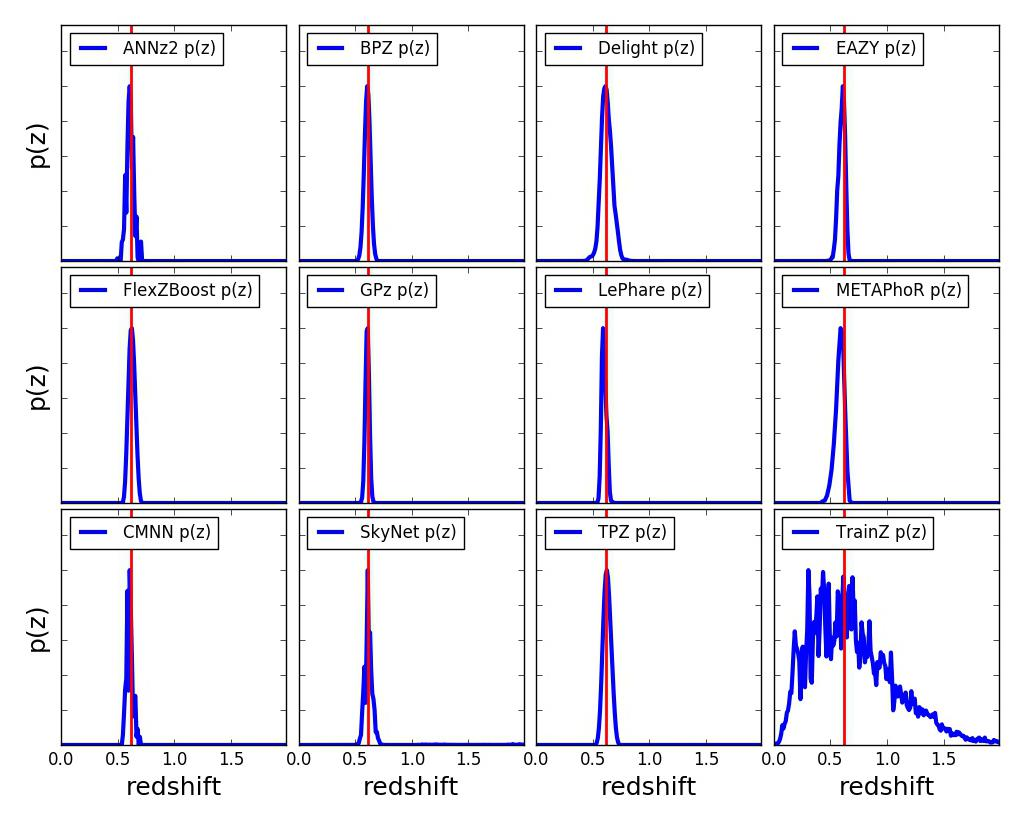
\includegraphics[width=0.49\textwidth]{figures/pzdc1/pz_12codes_261931_noseaborn_crop.jpg}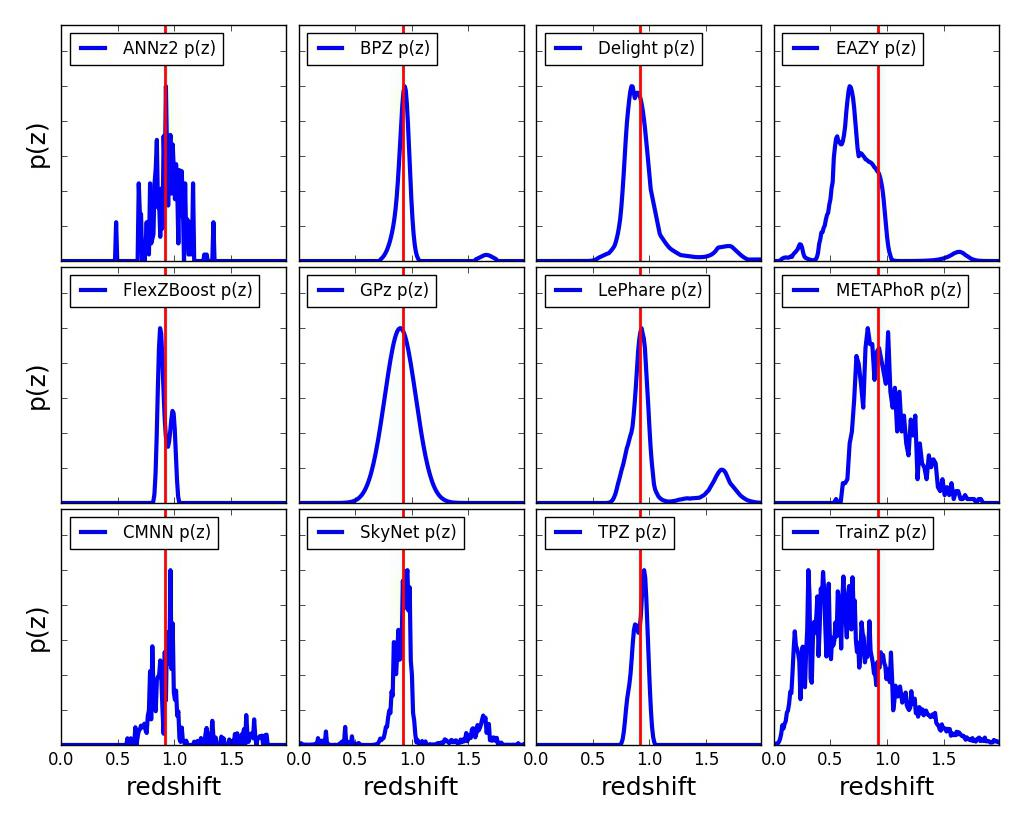
\includegraphics[width=0.49\textwidth]{figures/pzdc1/pz_12codes_471167_noseaborn_crop.jpg}\\
%	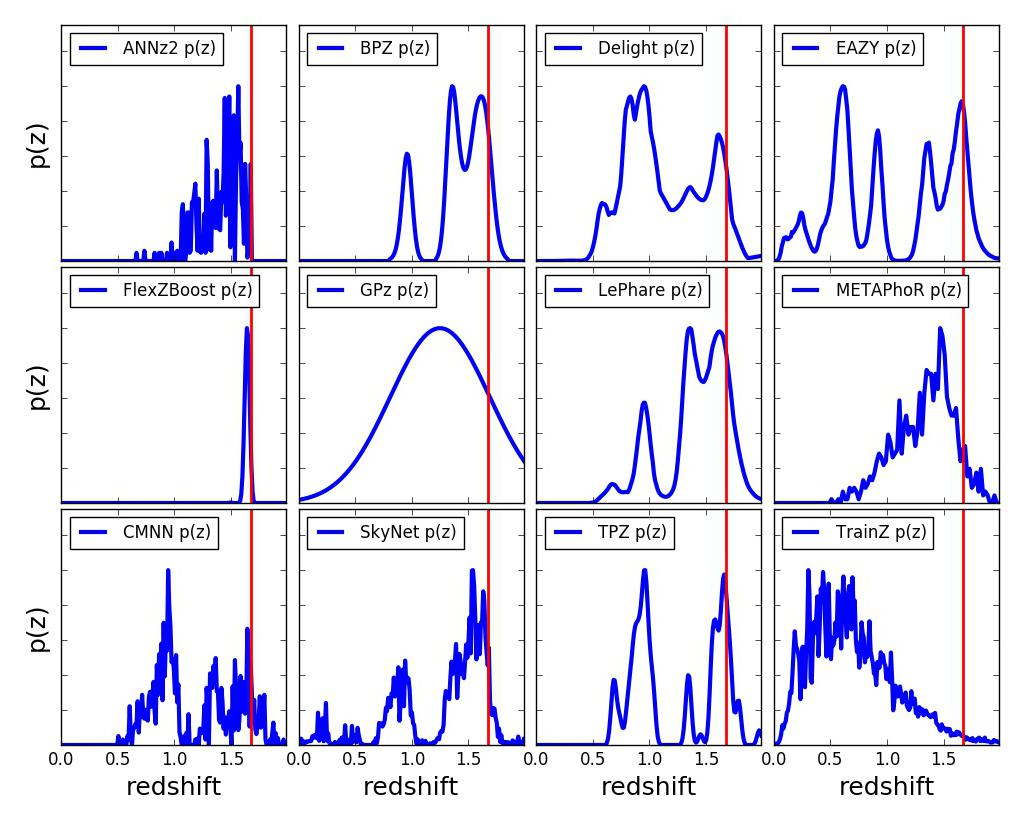
\includegraphics[width=0.49\textwidth]{figures/pzdc1/pz_12codes_713178_noseaborn_crop.jpg}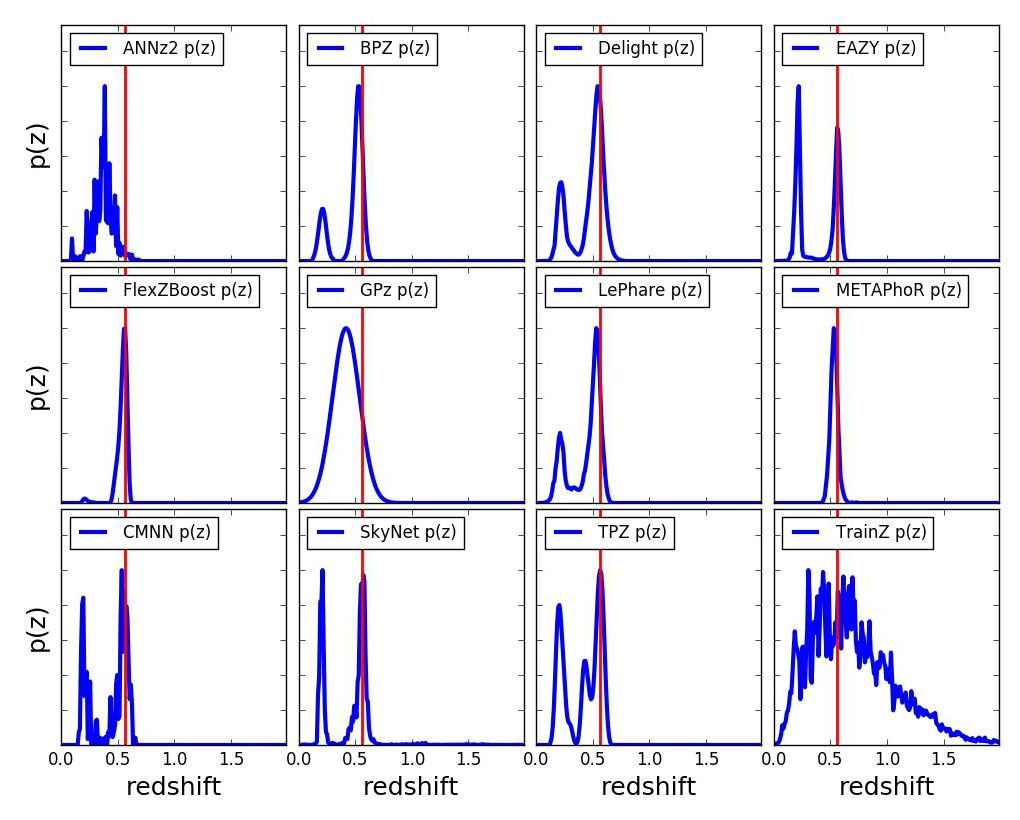
\includegraphics[width=0.49\textwidth]{figures/pzdc1/pz_12codes_982747_noseaborn_crop.jpg}
	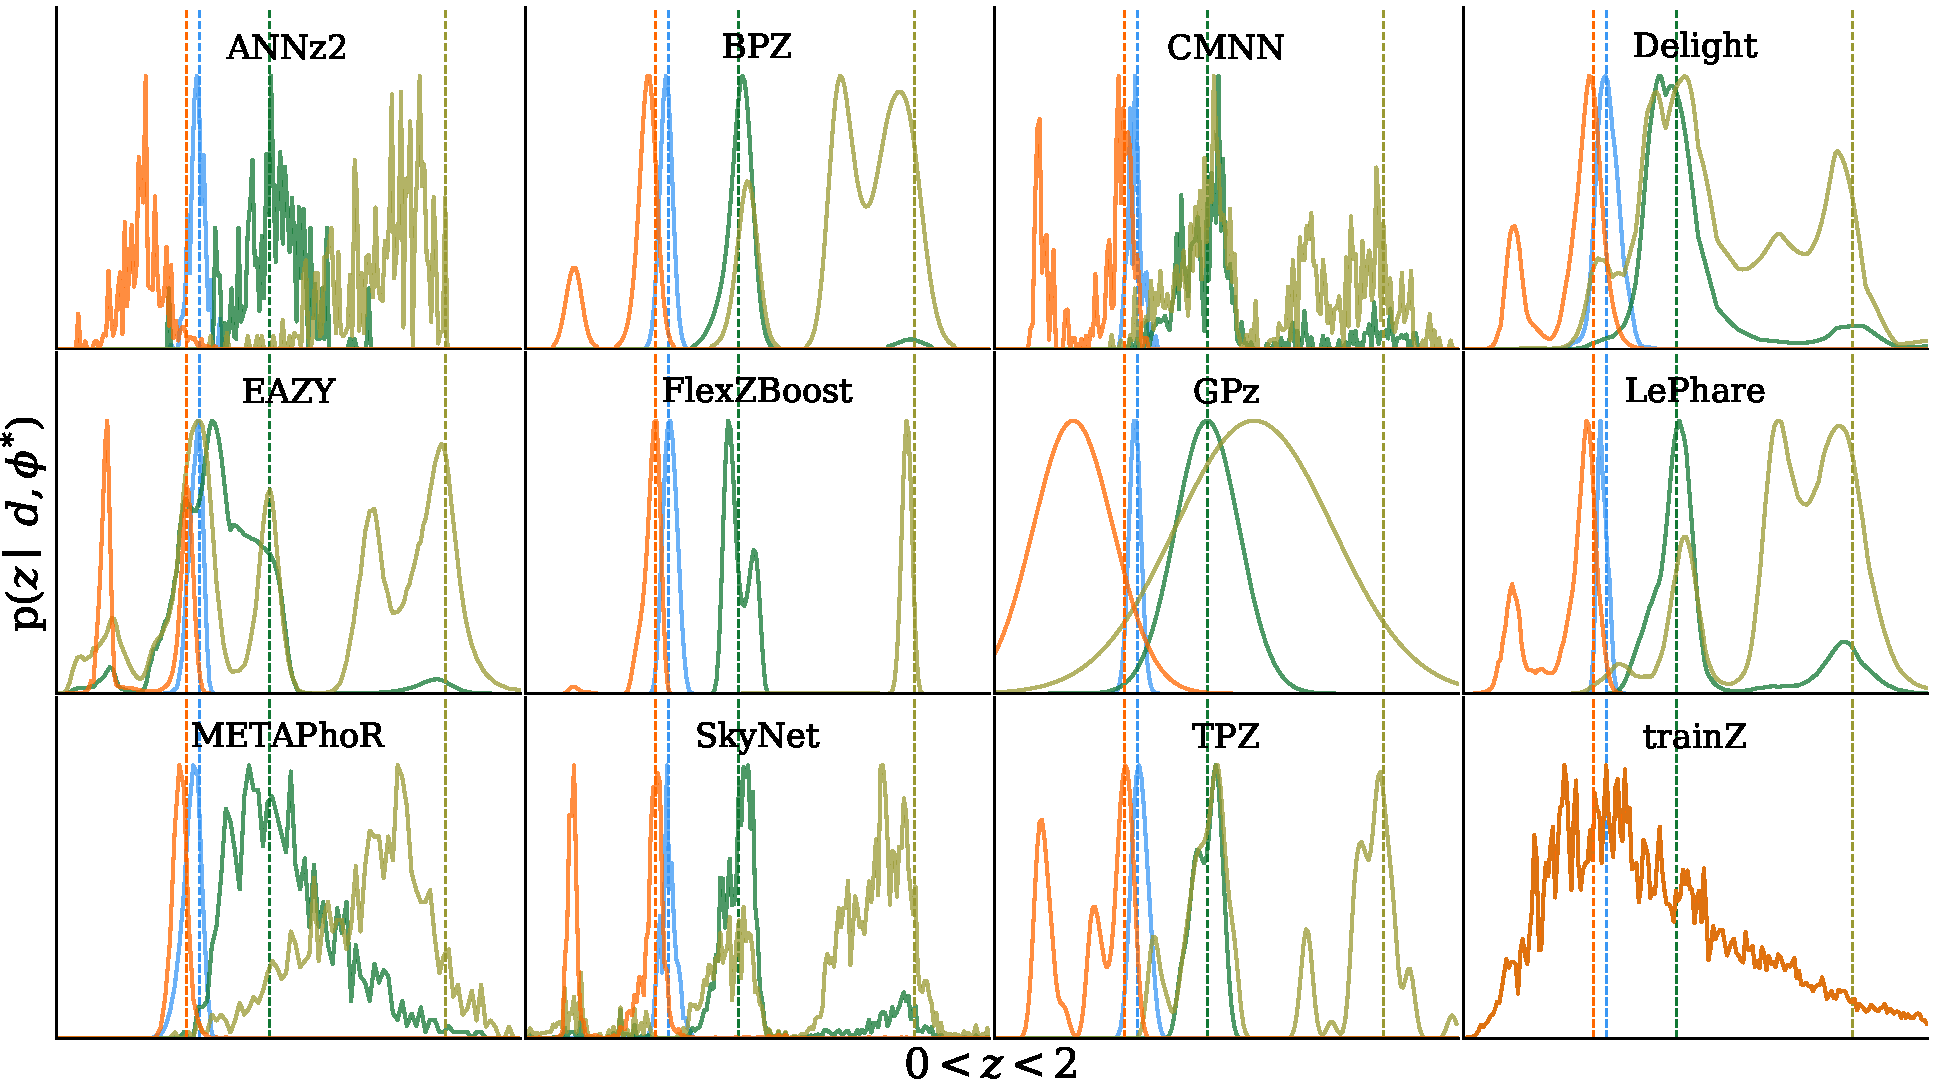
\includegraphics[width=\textwidth]{figures/pzdc1/EXAMPLE_pz_12codes_AIM.pdf}
	\caption{The individual \pzpdf s of four exemplary galaxies (colored curves) produced by the twelve codes (panels) with different true redshifts (vertical lines).
		The \pzpdf s of all codes share some features for the example galaxies due to physical color degeneracies and photometric errors: tight unimodal $p(z)$ (blue), broad unimodal $p(z)$ (green), bimodal $p(z)$ (orange), and complex/multimodal $p(z)$ (yellow).
		The diverse algorithms and implementations induce differences in small-scale structure and sensitivity to physical systematics.}
	\figlabel{fig:pz_examples}
\end{figure*}

The most striking differences between codes are due to small-scale features induced by the interaction between the shared piecewise constant parameterization of $200$ bins $0 < z < 2$ of \Sect{sec:metrics} and the smoothing conditions or lack thereof in each algorithm.
The $\rm{d}z = 0.01$ redshift resolution is sufficient to capture the broad peaks of faint galaxies' \pzpdf s with large photometric errors but is too broad to resolve the narrow peaks for bright galaxies' \pzpdf s with small photometric errors.
This observation is consistent with the findings of \citet[]{malz_approximating_2018} that the piecewise constant parameterization underperforms in the presence of small-scale structures.

However, the shared small-scale features of \annz, \metaphor, \cmnn, and \skynet\ are a result of various weighted sums of the limited number of training set galaxies with colors similar to those of the test set galaxy in question, with behavior closer to classification than regression in the case of \annz.
The settings used on \gpz\ in this work forced broadening of the single Gaussian to cover the multimodal redshift solutions of the other codes.
%Interestingly, while \textsc{ANNz2} shows an abundance of small scale structure in individual $p(z)$ measurements (see Fig.~\ref{fig:pz_examples}), the summed $\hat{N}(z)$ is rather smooth, where the small scale features average out.  This is not the case for the two other codes that show an abundance of substructure in their individual $p(z)$: both \textsc{CMNN} and \textsc{SkyNet} show small scale features both in $p(z)$ and $\hat{N}(z)$.
%In contrast, FlexZBoost, for example, can return estimates on any grid without compression errors as it’s a basis expansion method where only the expansion coefficients need to be stored.
%Codes with a native output format other than the shared piecewise constant binning scheme (or one that can be losslessly converted to it) may suffer from loss of information when converting to it, which could artificially favor some codes over others in a limited number of cases, for example bright galaxies with very narrow $p(z)$ where the true peak falls between grid points.  We will discuss PDF storage in Section~\ref{sec:discussion}.
%Furthermore, the fidelity of photo-$z$ interim posteriors in this format varies with the quality of the photometry.
%Switching to a quantile based parameterization may be more costly computationally, for example template-based codes would need to test more grid point in order to resolve the quantiles for bright galaxies.  However, the computational time for template based codes scales roughly linearly with the number of grid points, so this may be a reasonable thing to implement.
% We will discuss this further in Section~\ref{sec:discussion}.
% \red{someone review this statement to make sure that I'm saying this correctly!}

\subsection{Performance on \pzpdf\ ensembles}
\sectlabel{sec:pitqq}

The histogram of PIT values, QQ plot, and QQ difference plot relative to the ideal diagonal are provided in \Fig{fig:pitqq}, showcasing the biases and trends in the average accuracy of the \pzpdf s for each code.
The high QQ values (more high than low PIT values) of \bpz, \cmnn, \delight, \eazy, and \gpz\ indicate \pzpdf s biased low, and the low QQ values (more low than high PIT values) of \skynet\ and \tpz\ indicate \pzpdf s biased high.

\begin{figure*}
	\centering
	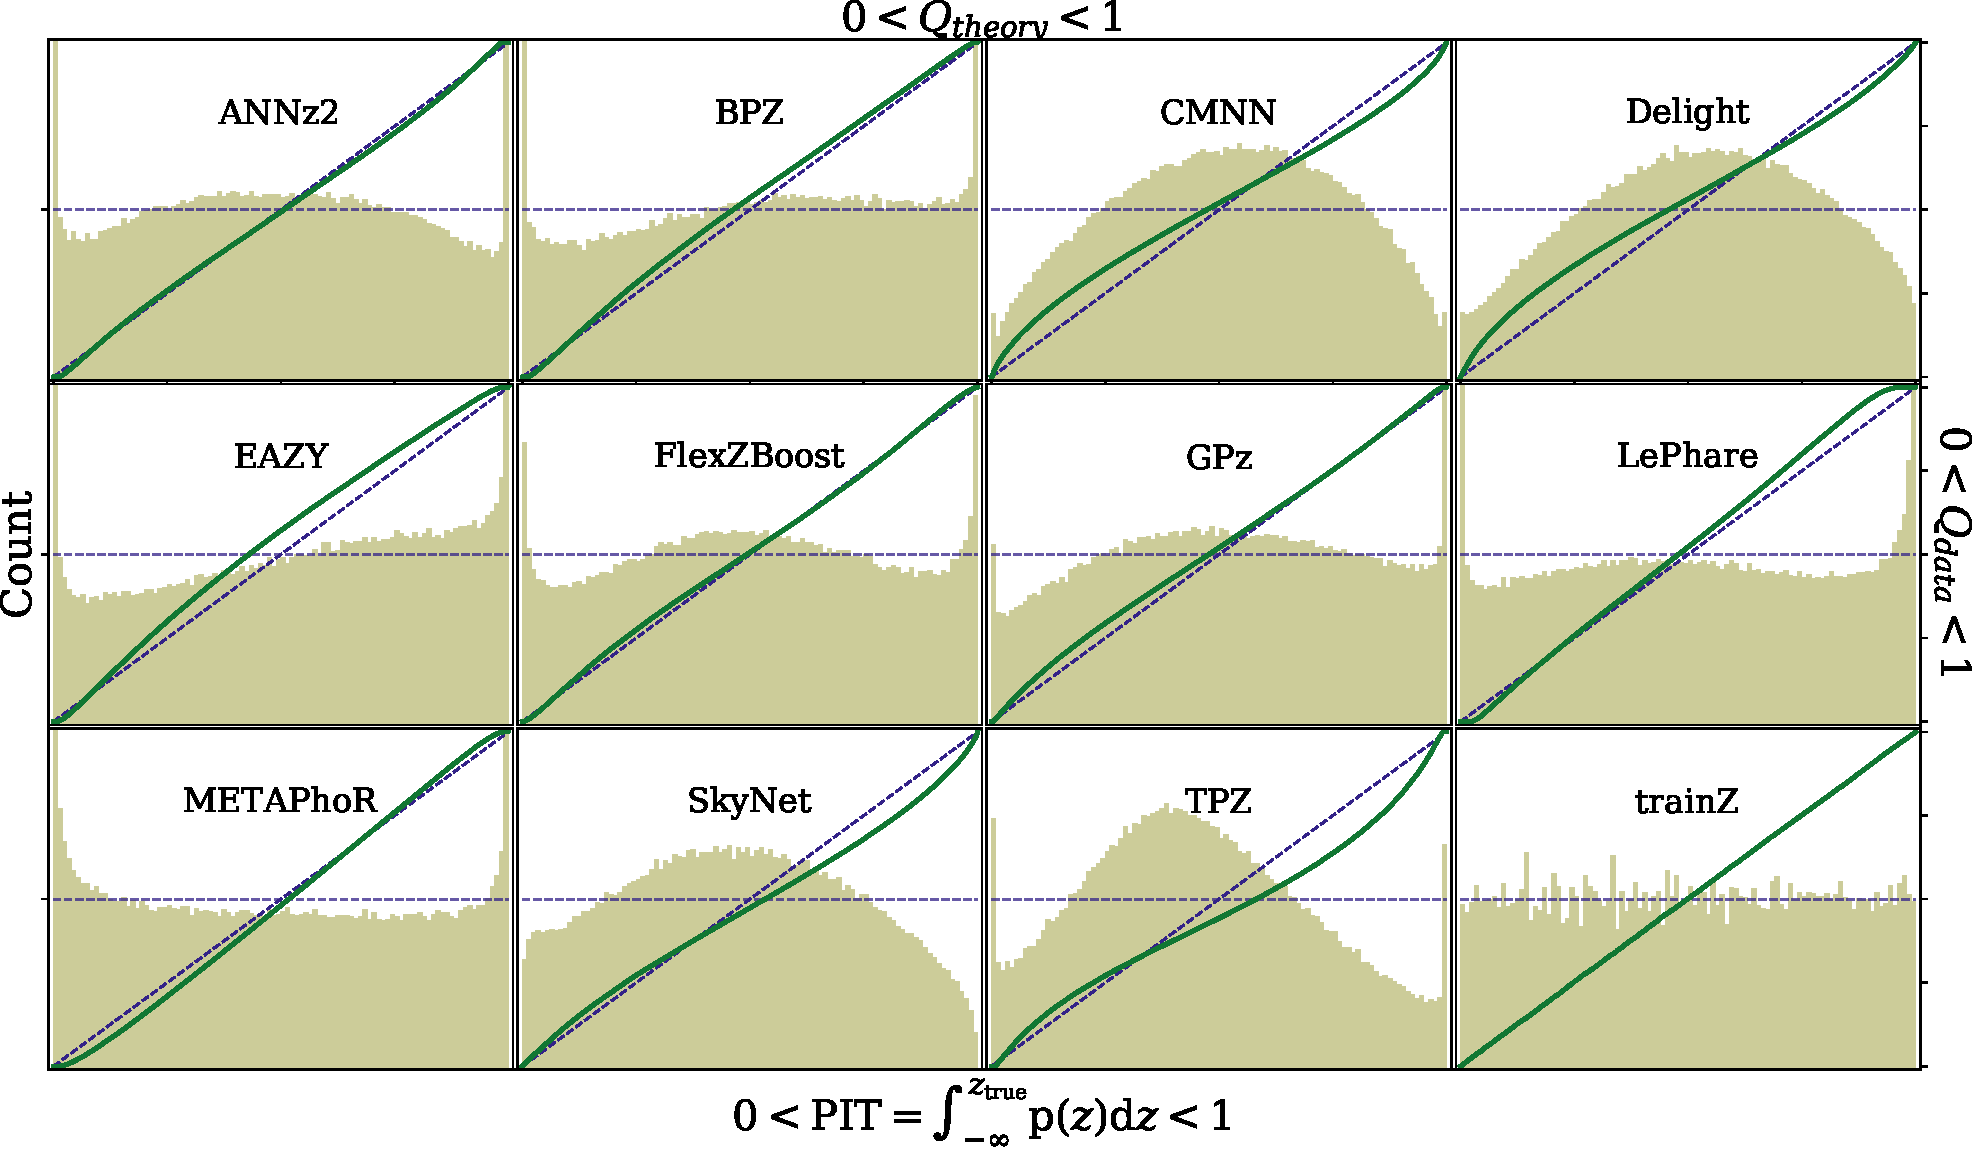
\includegraphics[width=\textwidth]{figures/pzdc1/PITQQcombo_12codes_AIM.pdf}
	\caption{The QQ plot (green curve) and PIT histogram (yellow bars) of the \pzpdf\ codes (panels) along with the ideal QQ (purple dashed diagonal) and ideal PIT (purple dashed horizontal) curves.
%		\aim{Add back the difference of the QQ from the ideal diagonal.}
		The twelve codes exhibit varying degrees of four deviations from perfection: an overabundance of PIT values at the centre of the distribution indicate a catalogue of overly broad \pzpdf s, an excess of PIT values at the extrema indicates a catalogue of overly narrow \pzpdf s, catastrophic outliers manifest as overabundances at PIT values of 0 and 1, and asymmetry indicates systematic bias, a form of model misspecification.}
	\figlabel{fig:pitqq}
\end{figure*}

The PIT histograms of \delight, \cmnn, \skynet, and \tpz\ feature an underrepresentation of extreme values, indicative of overly broad \pzpdf s, while the overrepresentation of extreme values for for \metaphor indicate overly narrow \pzpdf s.
These five codes in particular have a free parameter for bandwidth, which may be responsible for this vulnerability, in spite of the opportunity for fine-tuning with perfect prior information.
\flexzboost's ``sharpening'' parameter (described in \Sect{sec:flexzboost}) played a key role in diagonalizing the QQ plot, indicating a common avenue for improvement in the approaches that share this type of parameter.
On the other hand, the three purely template-based codes, \bpz, \eazy, and \lephare, do not exhibit much systematic broadening or narrowing, which may indicate that complete template coverage effectively defends from these effects.

\begin{table}
	\setlength{\tabcolsep}{2pt}
	\centering
	\caption{The catastrophic outlier rate as defined by extreme PIT values.
		We expect a value of 0.0002 for a proper Uniform distribution.
		An excess over this small value indicates true redshifts that fall outside the non-zero support of the $p(z)$.}
	\tablabel{tab:pitoutlier}
	\begin{tabular}{lc}
		\hline
		\hline
		\Pz\ Code & fraction PIT$<10^{-4}$ or $>$0.9999\\
		\hline
		\annz       & 0.0265\\
		\bpz        & 0.0192\\
		\delight    & 0.0006\\
		\eazy       & 0.0154\\
		\flexzboost & 0.0202\\
		\gpz        & 0.0058\\
		\lephare    & 0.0486\\
		\metaphor   & 0.0229\\
		\cmnn       & 0.0034\\
		\skynet     & 0.0001\\
		\tpz        & 0.0130\\
		\hline
		\trainz     & 0.0002
	\end{tabular}
\end{table}

Though the spikes in the first and last bin of the PIT histogram were cut off in \Fig{fig:pitqq} for visualization, the catastrophic outlier rates are provided in \Tab{tab:pitoutlier}.
As expected, \trainz\ achieves precisely the 0.0002 value expected of an ideal PIT distribution.
\annz, \flexzboost, \lephare, and \metaphor\ have notably high catastrophic outlier rates $> 0.02$, exceeding 100 times the ideal PIT rate, meriting further investigation.

\begin{figure*}
	\centering
	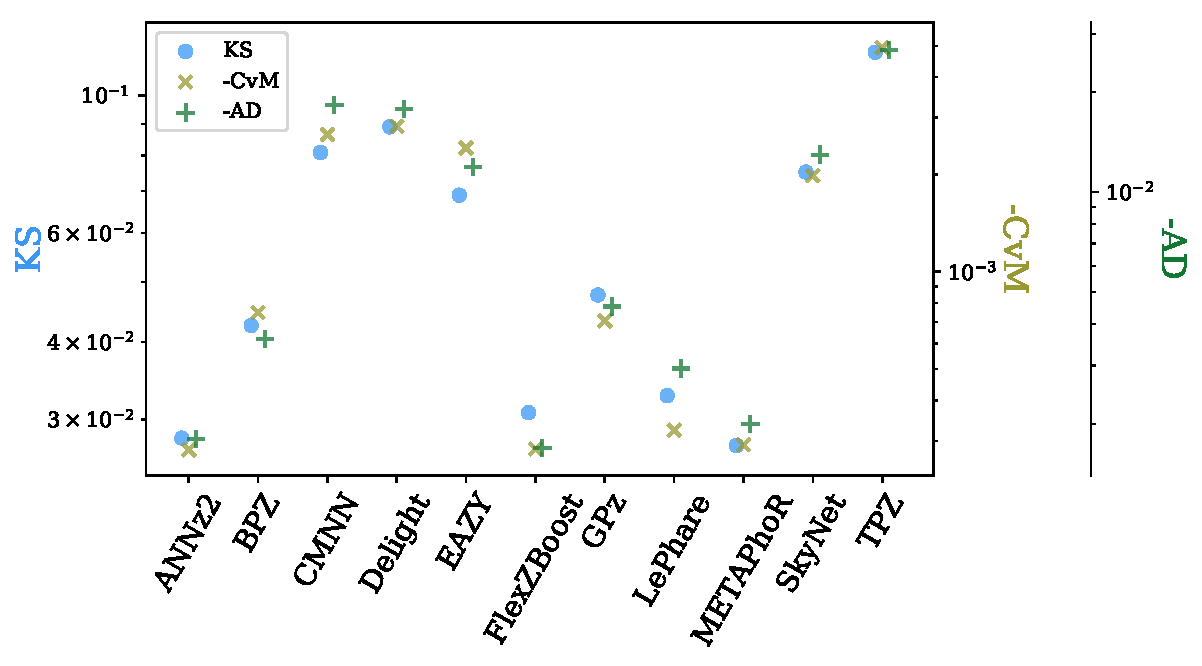
\includegraphics[width=0.74\textwidth]{figures/pzdc1/KSvsCvMvsAD_PIT.pdf}
	\caption{A visualization of the Kolmogorov-Smirnoff (KS, blue $\bullet$), Cramer-von Mises (CvM, yellow $\times$), and Anderson-Darling (AD, green $+$) statistics for the PIT distributions.
		There is generally good agreement between these statistics, with differences corresponding to the codes with outstanding catastrophic outlier rates, a reflection in the differences in how each statistic weights the tails of the distribution.}
	\figlabel{fig:pit_stats}
\end{figure*}

\Fig{fig:pit_stats} displays the values of the KS, CvM, and AD test statistics between the PIT distribution and a uniform distribution $U(0, 1)$, highlighting the relative rather than absolute numbers.
%\red{Can p-values be supplied for each statistic? The statistics themselves are difficult to interpret, other than ``lower is better'' (p-value in skgof was broken, having trouble finding 1-sample KS calculation for uniform distribution)}
\metaphor\ and \lephare\ perform well under the AD but poorly under the KS and CvM due to their high catastrophic outlier rates.
\annz\ and \flexzboost\  are the top scorers under these metrics of the PIT distribution.
\annz's strong performance can be attributed to an aspect of the training process in which training set galaxies with a PIT that more closely matches the percentiles of the DC1 training set's redshift distribution are upweighted; in effect, these quantile-based metrics were part of the algorithm itself that may or may not serve it well under more realistic experimental conditions.

\subsection{Performance on individual \pzpdf s}
\sectlabel{sec:cdelossresults}

The values of the CDE loss statistic of individual \pzpdf\ accuracy are provided in \Tab{tab:cdeloss}.
It is worth noting that strong performance on the CDE loss should imply strong performance on the other metrics, though the inverse is not necessarily true.
Thus the CDE loss is the most effective metric for generic science cases.

\begin{table}  %%% DATA TABLE %%%
	\centering
	\caption{CDE loss statistic of the individual \pzpdf s for each code.
		A lower value of the CDE loss indicates more accurate individual \pzpdf s, with \cmnn\ and \flexzboost\ performing best under this metric.}
	\tablabel{tab:cdeloss}
	\begin{tabular}{lr}
		\hline
		Photo-$z$ Code & CDE Loss \\
		\hline
		\annz 	    & $-6.88$ \\
		\bpz 		    & $-7.82$ \\
		%\textsc{Delight} 	& $-4.06$ \\
		\delight    & $-8.33$\\
		%\textsc{EAZY} 		& $-7.97$ \\
		\eazy       & $-7.07$ \\
		%\textsc{FlexZBoost} & $-11.51$ \\
		\flexzboost & $-10.60$\\
		\gpz		    & $-9.93$ \\
		\lephare 	  & $-1.66$ \\
		\metaphor 	& $-6.28$ \\
		%\textsc{CMNN} 		& $-$ \\
		\cmnn       & $-10.43$ \\
		\skynet 	  & $-7.89$ \\
		\tpz 		    & $-9.55$ \\
		\hline
		\trainz		  & $-0.83$ \\
		%\textsc{Frankenz}	& $-$  \\
		%\hline
	\end{tabular}
\end{table}

This metric is the only one that can appropriately penalize \trainz\ and indicates strong performance for \cmnn\ and \flexzboost, the latter of which is optimized for this metric.
%Empirically, we have found that PIT RMSE is not as closely correlated to CDE loss as it is to the $N(z)$ statistics.

\section{Discussion \& Future Directions}
\sectlabel{sec:discussion}
%(Sam Schmidt, Ofer Lahav, Jeff Newman, Alex Malz, Eve Kovacs, Tony Tyson, Tina Peters)

% If methods can not reach the goals on idealized data, then they will almost surely not meet those same goals when the more complex problems that we expect to arise from real LSST data are included.
% The results presented in this paper enable an evaluation of which algorithms are the most promising moving forward, and potentially point to avenues for improvement.

In contrast with other \pzpdf\ comparison papers that have aimed to identify the ``best'' code for a given survey, we have focused on the somewhat more philosophical questions of how to assess \pzpdf\ methods and how to interpret differences between codes in terms of \pzpdf\ performance.
In \Sect{sec:caution}, we reframe the strong performance of our pathological \pzpdf\ technique, \trainz, as a cautionary tale about the importance of choosing appropriate comparison metrics.
In \Sect{sec:futureexperiments}, we outline the experiments we intend to build upon this study
In \Sect{sec:futuredata}, we discuss the enhancements of the mock data set that will be necessary to enable the future experiments.

\subsection{Interpretation of metrics}
\sectlabel{sec:caution}
%(Alex Malz, Sam Schmidt)

We remind the reader that contributed codes were given a goal of obtaining accurate \pzpdf s, not an accurate stacked estimator of the redshift distribution, so we do not expect the same codes to necessarily perform well for both classes of metrics.
Indeed, the codes were optimized for their interpretation of our request for ``accurate \pzpdf s,'' and we expect that the implementations would have been adjusted had we requested optimization of the traditional metrics of \Sect{sec:moments} and \Sect{sec:pointmetrics}.

Furthermore, our metrics are not necessarily able to assess the fidelity of individual \pzpdf s relative to true posteriors.
Metric-specific performance implies that we may need multiple \pzpdf\ approaches tuned to each metric in order to maximize returns over all science cases in large upcoming surveys.

The \trainz\ estimator of \Sect{sec:trainz}, which assigns every galaxy a \pzpdf\ equal to $N(z)$ of the training set, is introduced as an experimental control or null test to demonstrate this point via \textit{reductio ad absurdum}.
Because our training set is perfectly representative of the test set, $N(z)$ should be identical for both sets down to statistical noise.
\textit{We make the alarming observation that \trainz\ outperforms all codes on the PIT-based metrics, and all but one code on the $N(z)$ based statistics.}
%\textit{Explain the connection between \trainz\ and these metrics.}

The CDE loss and point estimate metrics appropriately penalize \trainz's naivete.
As shown in \Sect{sec:pointmetrics}, \trainz ~has identical $ZPEAK$ and $ZWEIGHT$ values for every galaxy, and thus the \pz\ point estimats are constant as a function of true redshift, i.e. a horizontal line at the mode and mean of the training set distribution respectively.
The explicit dependence on the individual posteriors in the calculation of the CDE loss, described in \Sect{sec:cdelossresults}, distinguishes this metric from those of the \pzpdf\ ensemble and stacked estimator of the redshift distribution, despite their prevalence in the \pz\ literature.

% While looking at one, or even most of our metrics would have given the impression that this estimator was nearly optimal, red flags in CDE loss and point estimates reveal the problems.
%[more caution on over-reliance on metrics, and making sure that metrics test all of what you want] \red{this definitely still needs work}
In summary, context is crucial to defending against deceptively strong performers such as \trainz; \textbf{the best \pzpdf\ method is the one that most effectively achieves our science goals}, not the one that performs best on a metric that does not reflect those goals.
In the absence of a single scientific motivation or the information necessary for a principled metric definition, we must consider many metrics and be critical of the information transmitted by each.
% As stated earlier, science applications may be sensitive to individual \pzpdf s, \pzpdf\ ensembles, \pz\ point estimates, or science-specific statistics like $\hat{N}(z)$.
% We must be aware of that the optimal method for one is not necessarily optimal for the other, and in fact several photo-$z$ algorithms may be necessary in the final cosmological analysis in order to satisfy the requirements of all science use cases.
% The example of the simple \trainz\ estimator described in Section~\ref{sec:caution} shows a simple model with a $p(z)$ that is unrealistic for individual objects can still score very well on many of our metrics.
% It is important to look at {\it all} metrics, and keep in mind what information each metric conveys.
%\aim{[reiterate the meaning of $p(z)$ and the goal -- emphasize finding ``best'' code in terms of impact of assumptions underlying the method \textit{or} establishing methodology for the realistic case of biased prior information and other science goals]}
%\red{[the challenges faced in this project]}
%\red{mention z$<$2, missing some important degeneracies, new sim will go to higher z}
%\red{no quality cuts included, could identify outliers, but could also induce biases}
%\red{[how optimization defined has impact, here we optimized p(z), not n(z), could be science-case specific if stringent requirements are needed, though that may be a computational/storage challenge if too many use cases needed.]}
%\red{some discussion of output parameterization, limitations of 200 point fixed grid, in future switch to something like quantiles (cite qp paper)}

\subsection{Extensions to the experimental design}
\sectlabel{sec:futureexperiments}

%\begin{enumerate}
%\item \red{the combination of codes}
%\item \red{$p(z,\alpha)$}
%\item \red{tomographic analysis later on}
%\red{this paper deals with training, future papers will also explore calibration via cross-correlation methods}
%\end{enumerate}
%\red{mention the SRM once again, say that the plans are extensive, but we do have a plan and a rough timeline.}

The work presented in this paper is only a first step in assessing \pzpdf\ approaches and moving toward an improved photometric redshift estimator.
Here we discuss the next steps for subsequent investigations.

This initial paper explored code performance in idealized conditions with perfect catalog-based photometry and representative training data.
A top priority for a follow-up study is to test realistic forms of incomplete, erroneous, and non-representative template libraries and training sets as well as the impact of other forms of external priors that must be ingested by the codes, major concerns in \citet{Newman:2015, Masters:2017}.
We plan to perform a full sensitivity analysis on a realistically incomplete training set of spectroscopic galaxies, modeling the performance of spectrographs, emission-line properties, and expected signal-to-noise to determine which potential training set galaxies are most likely to be excluded.
In addition to outright redshift failures we will model the inclusion of a small number of high-confidence yet false redshifts due to emission line misidentification or noise spikes.

\Sect{sec:moments} only addresses the stacked estimator of the redshift distribution of the entire galaxy catalogue rather than subsets in bins, tomographic or otherwise.
The effects of tomographic binning scheme will be explored in a dedicated future paper, including propagation of redshift uncertainties in a set of fiducial tomographic redshift bins in order to estimate impact on cosmological parameter estimation.

%\red{[are there any references for this?  I remember Gary Bernstein talking about this at a photo-z workshop in Japan, but I don't know that it was published.  I believe Michael Troxel has discussed this as well.]}
%\item \red{cosmological parameters in DC2}
%\item \red{mention z$<$2, missing some important degeneracies, new sim will go to higher z}
%\red{no quality cuts included, could identify outliers, but could also induce biases}

Sequels to this study will also address some shortcomings of our experimental procedure.
The fixed redshift grid shared between the codes may have unfairly penalized codes with a different native parameterization, as precision is lost when converting between formats.
Performance on sharply peaked \pzpdf s may have been suppressed across all codes due to the insufficient resolution of the redshift grid.
In light of the results of \citet[]{malz_approximating_2018}, in future analyses we plan to switch from a fixed grid to the quantile parameterization or to permit each code to use its native storage format under a shared number of parameters.

\subsection{Realistic mock data}
\sectlabel{sec:futuredata}

To make optimal use of the \lsst\ data for cosmological and other astrophysical analyses of the Science Roadmap, future investigations that build upon this one will require a more sophisticated set of galaxy photometry and redshifts.
%\item \red{inclusion of photometric errors, image based effects, blending, lensing, sky, mask, etc...}
This initial paper explored a data set that was constructed at the catalog level, with no inclusion of the complications that come from measuring photometry from images.
Future data challenges will move to catalogs constructed from mock images, including the complications of deblending, sensor inefficiencies, and heterogeneous observing conditions, all anticipated to affect the measured colours of \lsst's galaxy sample \citep{Dawson:2016}.

The DC1 galaxy SEDs were linear combinations of just five basis SED templates, but a next generation of data for \pzpdf\ investigations must include a broader range of physical properties.
Though we only considered $z < 2$ here, \lsst\ 10-year data will contain $z > 2$ galaxies, plagued by fainter apparent magnitudes and anomalous colours due to stellar evolution.
A subsequent study must also have a data set that includes low-level active galactic nuclei (AGN) features in the SEDs, which perturb colours and other host galaxy properties.
An observational degeneracy between the Lyman break of a $z \sim 2-3$ galaxy from the Balmer break of a $z \sim 0.2-0.3$ galaxy is a known source of catastrophic outliers \citep{Massarotti:2001} that was not effectively included in this study.
To gauge the sensitivity of \pzpdf\ estimators to catastrophic outliers, our data set must include realistic high-redshift galaxy populations.

% In this study we have not accounted for the presence of Active Galactic Nuclei (AGN) contributions to galaxy fluxes.
% In some cases, AGN will be easily identified from the colors and morphologies, i.e. the case of the brightest quasars where the nuclear activity outshines the host galaxy, and numerous studies have utilized color selection to create large samples of quasars \citep[e.g.][]{Richards:06,Maddox:08,Richards:15}.
% In current deep fields, similar in depth to what we expect from \lsst, variability information and multi-wavelength data have been critical to not only identify AGN dominated galaxies, but also obtain more accurate photometric redshifts \citep[e.g][]{Salvato:11}.
%
% In addition to AGN dominated galaxies, those with lower levels of nuclear activity present a more insidious problem, where AGN features may not be apparent, but the colours and other host galaxy properties are perturbed relative to galaxies with an inactive nucleus.
% In such cases, the presence of the AGN may induce a bias if the template SEDs or empirical datasets do not include low-level AGN counterparts.
% For LSST, we will need to identify and obtain accurate photometric redshifts of all types of AGN for a range of science goals, whether it is to eliminate such objects from cosmology experiments, or to use them with confidence, all the way through to understanding galaxy evolution and the role that AGN may play in influencing galaxy properties over cosmic time.

% A promising route to classifying and obtaining accurate photometric redshifts for the AGN population is by combining machine learning with template-fitting techniques, as has recently been demonstrated by \citet{Duncan:18} for radio-selected AGN.
% This is because AGN are relatively easy to obtain spectroscopic redshifts for over all redshifts due to the strong emission lines that they exhibit, allowing very good training sets for machine learning algorithms to use.
% Whereas for those galaxies where the AGN is sub-dominant the galaxy templates are still adequate for obtaining reasonable photometric redshifts.

% In addition to these improvements, the \lsstdesc \Pz\ Working Group plans to look at all potential methods to combine the results from multiple \pzpdf\ codes to improve accuracy, similar to the work presented in \citet{Dahlen:13,Carrascokind:14,Duncan:18}.
% Taking advantage of multiple algorithms that use observables in slightly different ways has shown promise, however we must be very conscious of whether a potential combination properly treats the covariance between the methods, given that they are estimating quantities based on the same underlying observables.
% Several science cases wish to estimate physical quantities along with redshift, for example galaxy stellar mass and star formation rate.
% Proper joint estimation of redshift and physical quantities requires an in depth understanding of galaxy evolution, and progress on accurate bivariate redshift probability distributions will go hand in had with progress on understanding galaxies themselves.
% Parameterization and storage of a complex 2-dimensional probability surface for potentially billions of galaxies (or even subsets of hundreds of thousand of particular interest) pose a potential challenge.
% These issues will be examined in another future paper.

% Finally, while this paper and future papers discussed above focus on photometric redshift codes and estimating accurate \pzpdf s from training data, we plan a separate, but complementary, project to examine calibration of the resultant redshifts via spatial cross-correlations \citep{Newman:2008}, which will be explored in a separate series of future papers.
The overarching plan describing everything laid out in this section is described in more detail in the \desc\ Science Roadmap\footref{lsstdesc_srm}).

\section{Conclusion}
\sectlabel{sec:conclusion}
%(Sam Schmidt, Ofer Lahav, Jeff Newman, Alex Malz, Eve Kovacs, Tony Tyson, Tina Peters)

This paper compares twelve \pzpdf\ codes under controlled experimental conditions of representative and complete prior information to set a baseline for an upcoming sensitivity analysis.
This work isolates the impact on metrics of \pzpdf\ accuracy due to the estimation technique as opposed to the complications of realistic physical systematics of the photometry.
Though the mock data set of this investigation did not include true \pz\ posteriors for comparison, \textbf{we interpret deviations from perfect results given perfect prior information as the imprint of the implicit assumptions underlying the estimation approach}.

We evaluate the twelve codes under science-agnostic metrics both established and emerging to stress-test the ensemble properties of \pzpdf\ catalogues derived by each method.
In appendices, we also present metrics of point estimates and a prevalent summary statistic of \pzpdf\ catalogues used in cosmological analyses to enable the reader to relate this work to studies of similar scope.
We observe that no one code dominates in all metrics, and that the standard metrics of \pzpdf s and the stacked estimator of the redshift distribution can be gamed by a vacuously wrong procedure that asserts the prior over the data.
We emphasize to the \pz\ community that \textbf{metrics used to vet \pzpdf\ methods must be scrutinized to ensure they correspond to the quantities that matter to our science}.

\section*{Appendices}
\addcontentsline{toc}{section}{Appendices}
\renewcommand{\thesubsection}{\Alph{subsection}}

\subsection{Evaluation of the redshift distribution}
\label{sec:moments}
%(Alex Malz)

Perhaps the most popular application of \pzpdf s is the estimation of the overall redshift distribution $N(z)$, a quantity that enters some cosmological calculations and the true value of which is known for the DC1 data set and will be denoted as $\tilde{N}(z)$.
In terms of the prior information provided to each method, the true redshift distribution satisfies the tautology $\tilde{N}(z) = p(z \vert I_{D})$ due to our experimental set-up; because the DC1 training and template sets are representative and complete, $I_{D}$ represents a prior that is also equal to the truth.
In this ideal case of complete and representative prior information, the method that would give the best approximation to $\hat{N}(z)$ would be one that neglects all the information contained in the photometry $\{d_{i}\}_{N_{tot}}$ and gives every galaxy the same \pzpdf\ $\hat{p}_{i}(z) = \tilde{N}(z)$ for all $i$; the inclusion of any information from the photometry would only introduce noise to the optimal result of returning the prior.
This is the exact estimator, \trainz, that we have described in \Sect{sec:trainz}, and which will serve as an experimental control.

\subsubsection{Metrics of the stacked estimator of the redshift distribution}
\label{sec:stackedmetrics}

Though alternatives exist \citep{Malz:chippr}, ``stacking'' according to
\begin{equation}
\label{eq:stacked}
\hat{N}^{H}(z) \equiv \frac{1}{N_{tot}}\ \sum_{i}^{N_{tot}}\ \hat{p}^{H}_{i}(z)
\end{equation}
is the most widely accepted method for obtaining $\hat{N}^{H}(z)$ as an estimator of the redshift distribution from \pzpdf s derived by a method $H$.
Though we do not endorse the use of the stacked estimator of the redshift distribution, we use it under the untested assumption that the response of our metrics of $\hat{N}^{H}(z)$ will be analogous to the same metrics applied to a principled estimator of the redshift distribution.

As $N(z)$ is itself a univariate PDF, we apply the metrics of the previous sections to it as well.
We additionaly calculate the first three moments
\begin{equation}
\eqlabel{eq:moment}
\langle z^{m}\rangle \equiv \int_{-\infty}^{\infty} z^{m} N(z) dz
\end{equation}
of the estimated redshift distribution $\hat{N}^{H}(z)$ for each code and compare them to the moments of the true redshift distribution $\tilde{N}(z)$.
Under the assumption that the stacked estimator is unbiased, a superior method minimizes the difference between the true and estimated moments.

\subsubsection{Performance on the stacked estimator of the redshift distribution}
\label{sec:stackedmetrics_results}

\Fig{fig:nz} shows the stacked estimator $\hat{N}(z)$ of the redshift distribution for each code compared to the true redshift distribution $\tilde{N}(z)$, where the stacked estimator has been smoothed for each code in the plot using a kernel density estimate (KDE) with a bandwidth chosen by Scott's Rule \citep{Scott:1992} in order to minimize visual differences in small-scale features; the quantiative statistics, however, are calculated using the empirical CDF which is not smoothed.

\begin{figure*}
	\centering
	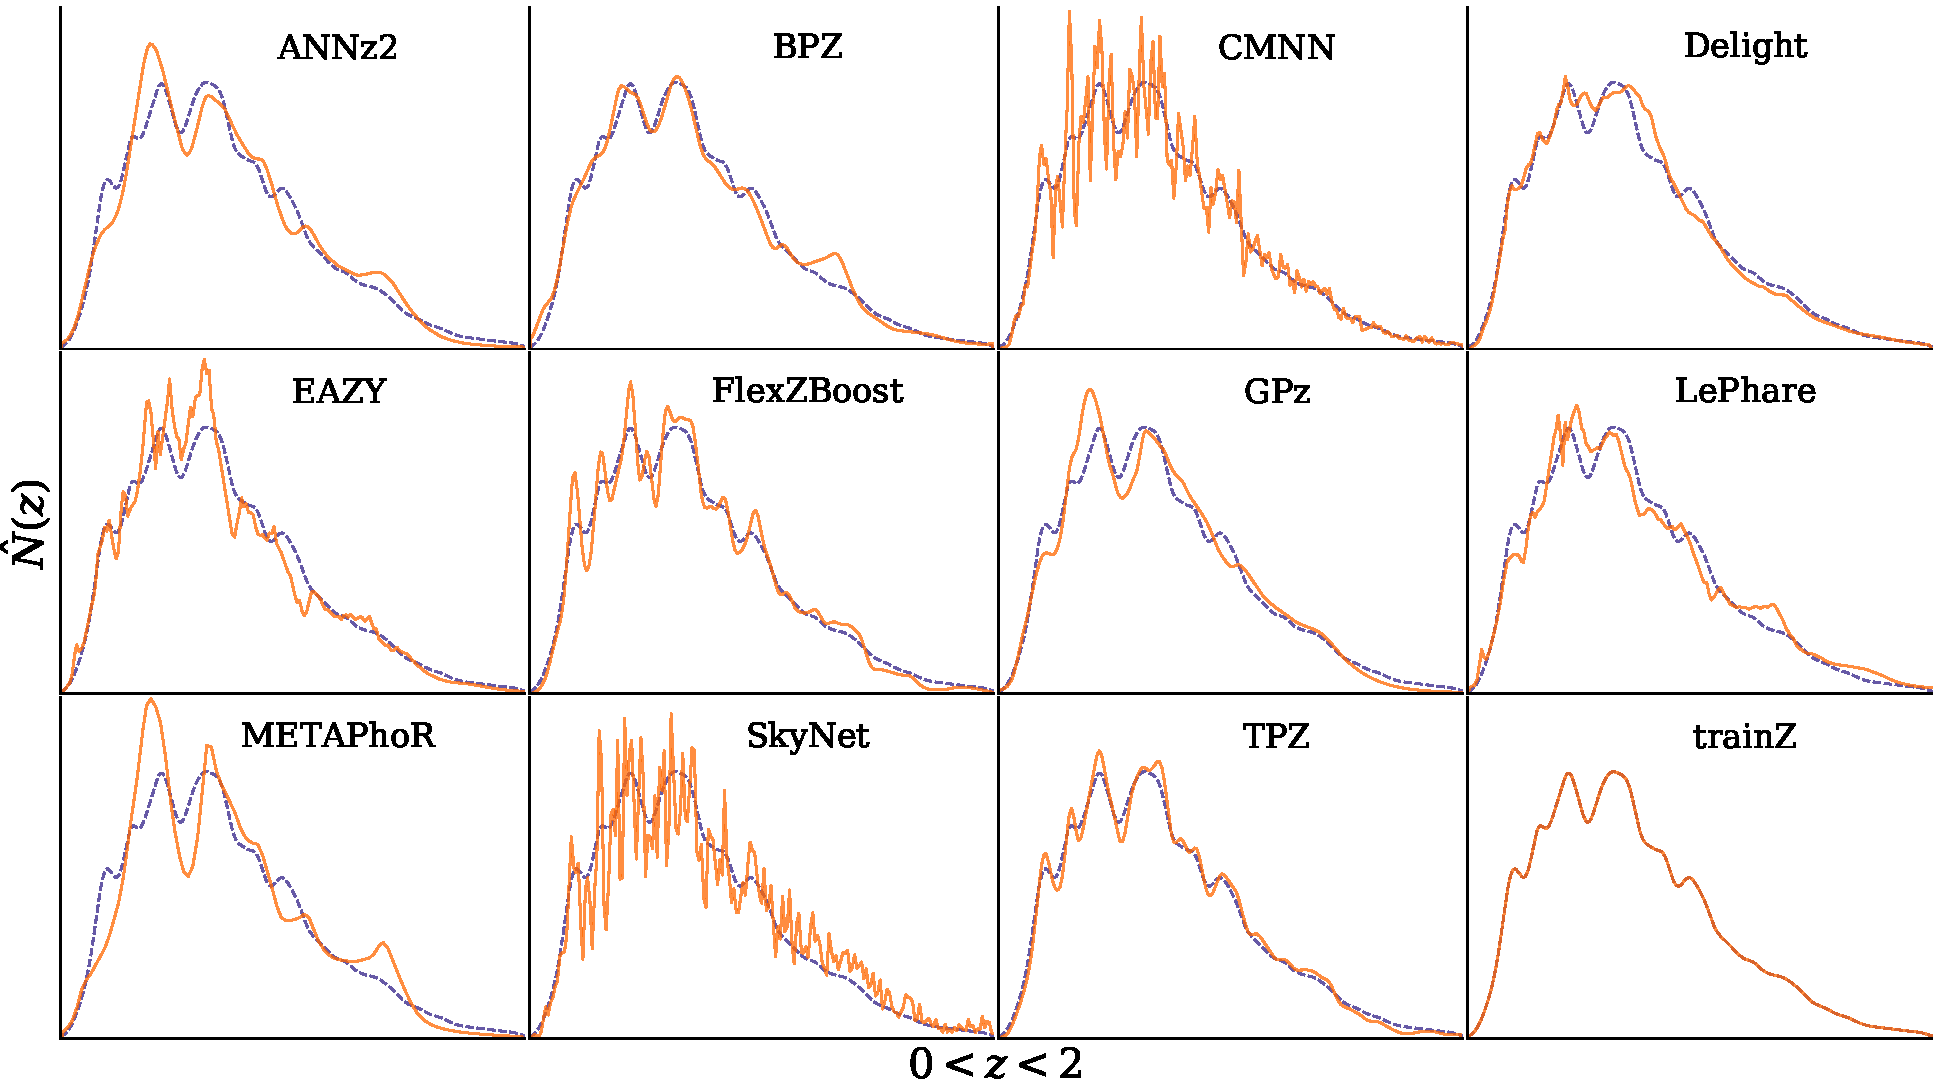
\includegraphics[width=\textwidth]{figures/pzdc1/NZsumplot_AIM.pdf}
	\caption{The smoothed stacked estimator $\hat{N}(z)$ of the redshift distribution (orange) produced by each code (panels) compared to the true redshift distribution $\tilde{N}(z)$ (purple dashed).
		Varying levels of agreement are seen among the codes, with the smallest deviations for \cmnn, \flexzboost, \tpz, and \trainz.}
	\figlabel{fig:nz}
	%\aim{Arguably this could also be clarified by showing the true $n'(z)$ once and then differences from it for each cod's stacked estimator\dots}\scc{what if we plot the difference between true and stacked rather than soverposing the two lines? Sam please do not hate me.}
\end{figure*}

Many of the codes, including all the model-fitting approaches and \annz, \gpz, \metaphor, and \skynet\ from the data-driven camp, overestimate the redshift density at $z \sim 1.4$.
This behavior is a consequence of the $4000 \rm{\AA}$ break passing through the gap between the $z$ and $y$ filters, which induces a genuine discontinuity in the $z - y$ colour as a function of redshift that can sway the \pzpdf\ estimates in the absence of bluer spectral features.

\annz, \gpz, and \metaphor\ show signs of overtraining, estimating enhanced peaks and diminished troughs relative to the training set, an obstacle that may be overcome with adjustment of the implementation.

As expected, \trainz\ perfectly recovers the true redshift distribution: as the training sample is selected from the same underlying distribution as the test set, the redshift distributions are identical, up to Poisson fluctuations due to the finite number of sample galaxies.
\cmnn\ is also in excellent agreement for similar reasons: with a representative training sample of galaxies spanning the colour-space, the sum of the colour-matched neighbour redshifts should return the true redshift distribution.
\flexzboost\ and \tpz\ also perform superb recovery of the true redshift distribution, with only a slight deviation at $z \sim 1.4$.
Our metrics, however, cannot discern whether these four approaches, as well as \delight, are spared the $z \sim 1.4$ degeneracy in $\hat{N}(z)$ because they have more effectively used information in the data or if the impact is simply washed out by the stacked estimator's effective average over the test set galaxy sample.
See \Sect{sec:pointmetrics} for further discussion of the $z \sim 1.4$ issue.

\Fig{fig:nz_stats} shows the quantitative Kolmogorov-Smirnoff (KS), Cramer-Von Mises (CvM), and Anderson Darling (AD) test statistics for each of the codes for the $\hat{N}(z)$ based measures.
%\red{Can p-values be supplied for each statistic? The statistics themselves are difficult to interpret, other than ``lower is better'' (no, p-values are very difficult to compute for non-uniform distributions)}
The stacked estimators of the redshift distribution for \cmnn\ and \trainz\ best estimate $\tilde{N}(z)$ under these metrics, and the only codes that do especially poorly are \eazy, \lephare, \metaphor, and \skynet.
It is unsurprising that \cmnn\ scores well, as with a near perfectly representative training set means that choosing neighbouring points in color/magnitude space should lead to excellent agreement in the final $\hat{N}(z)$ estimate.

\begin{figure*}
	\centering
	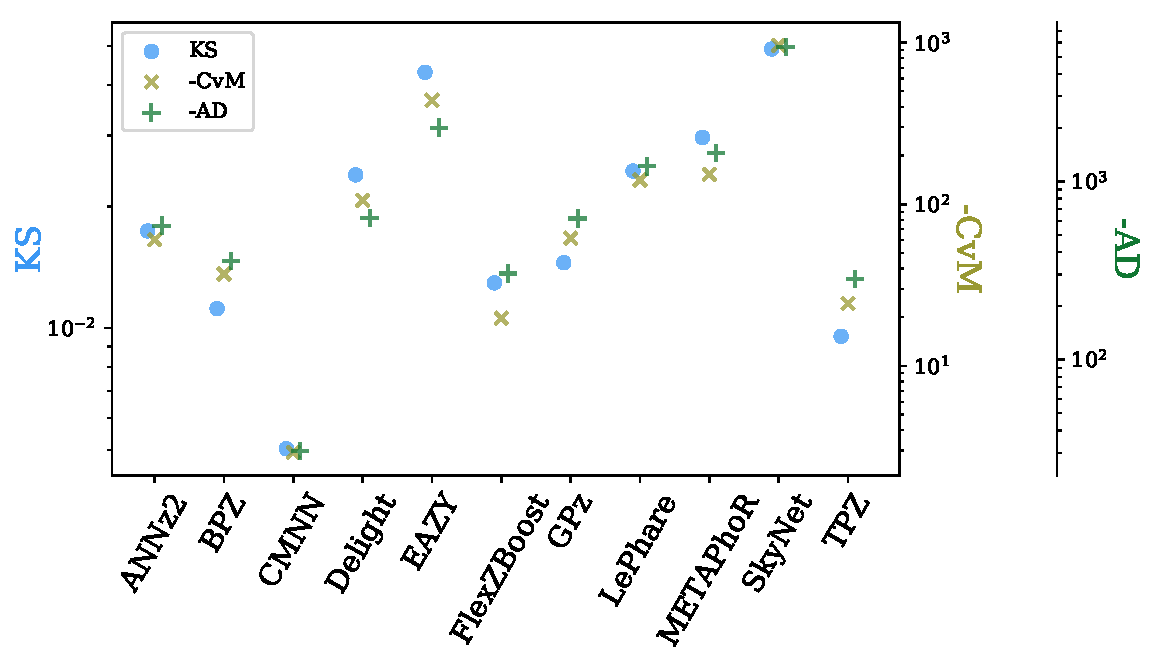
\includegraphics[width=0.74\textwidth]{figures/pzdc1/KSvsCvMvsAD_Nz.pdf}
	\caption{A visualization of the Kolmogorov-Smirnoff (KS, blue $\bullet$), Cramer-von Mises (CvM, yellow $\times$), and Anderson-Darling (AD, green $+$) statistics for the $\hat{N}(z)$ distributions.
		We make the reassuring observation that these related statistics do not disagree significantly with one another.
		\cmnn\ performs comparably well to \trainz, the control case, while \skynet\ scores poorly due to an overall bias in its redshift predictions.}
	\figlabel{fig:nz_stats}
\end{figure*}

It is, however, surprising that \tpz\ does well on $\hat{N}(z)$ given its poor performance on the ensemble \pzpdf s, especially knowing that \tpz\ was optimized for \pzpdf\ ensemble metrics rather than the stacked estimator of the redshift distribution.
A possible explanation is the choice of smoothing parameter chosen during validation, which affects \pzpdf\ widths as well as overall redshift bias and could be modified to improve performance under the \pzpdf\ metrics.

The first three moments of the stacked $\hat{N}(z)$ distribution relative to the empirical estimate of the truth distribution are given in \Tab{tab:moments}.
Accuracy of the moments varies widely between codes, raising concerns about the propagation to cosmological analyses.
%\red{[mention that we are calculating moments for the entire sample, will look at fiducial tomographic bins in a follow-up paper (unless group and reviewers realy think we should include in this paper.]}
%\red{FlexZBoost has some of the best $n(z)$ statistics, but the moments are not good.  Why is this?  Is it the over/underprediction of the high redshift part of the distribution?  Discuss this after talking with Rafael.}

\begin{table}
	\begin{center}
	\setlength{\tabcolsep}{2pt}
	\caption{Moments of the stacked estimator $\hat{N}(z)$ of the redshift distribution.
		Most of the codes considered recover the moments of $\tilde{N}(z)$}
	\tablabel{tab:moments}
	\begin{tabular}{lccc}
		\hline
		\hline
		\multicolumn{4}{l}{Moments of $\hat{N}(z)$} \\
		\hline
		Estimator  & mean       & variance    & skewness \\
		Empirical ``truth'' & 0.701 & 0.630 & 0.671  \\
		\hline
		\annz       & 0.702      & 0.625      & 0.653    \\
		\bpz        & 0.699      & 0.629      & 0.671    \\
		\delight    & 0.692      & 0.609      & 0.638    \\
		\eazy       & 0.681      & 0.595      & 0.619    \\
		\flexzboost & 0.694      & 0.610      & 0.631    \\
		\gpz        & 0.696      & 0.615      & 0.639    \\
		\lephare    & 0.718      & 0.668      & 0.741    \\
		\metaphor   & 0.705      & 0.628      & 0.657    \\
		\cmnn       & 0.701      & 0.628      & 0.667    \\
		\skynet     & 0.743      & 0.708      & 0.797    \\
		\tpz        & 0.700      & 0.619      & 0.643    \\
		\hline
		\trainz	    & 0.699 		 & 0.627 	    & 0.666 \\
	\end{tabular}
\end{center}
\end{table}

\skynet\ exhibits redshift bias in \Fig{fig:nz} and is a clear outlier in the first moment of $\hat{N}(z)$ in \Tab{tab:moments}.
The \skynet\ algorithm employs a random subsampling of the training set without testing that the subset is representative of the full population, and the implementation used here does not upweight rarer low- and high-redshift galaxies, as in \citet{bonnett_using_2015}, suggesting a possible cause that may be addressed in future work.

\subsection{\Pz\ point estimation and metrics}
\label{sec:allpointmetrics}

While this work assumes that science applications value the information of the full \pzpdf, we present conventional metrics of \pz\ point estimates as a quick and dirty diagnostic tool and to facilitate direct comparisons to historical studies.

\subsubsection{Reduction of \pzpdf s to point estimates}
\label{sec:pointest}

Though we acknowledge that many of the codes can also return a native \pz\ point estimate, we put all codes on equal footing by considering two generic \pz\ point estimators, the mode $z_{PEAK}$ and main-peak-mean $z_{WEIGHT}$ \citep{Dahlen:13}, a weighted mean within the bounds of the main peak, as identified by the roots of $p(z) - 0.05 \times z_{PEAK}$.
Though $z_{WEIGHT}$ neglects information in a secondary peak of a, say, bimodal distribution, it avoids the pitfall of reducing the \pzpdf\ to a redshift between peaks where there is low probability.

\subsubsection{Metrics of \pz\ point estimates}
\sectlabel{sec:pointmetrics}

We calculate the commonly used point estimate metrics of the overall intrinsic scatter, bias, and catastrophic outlier rate, defined in terms of the standard error $e_{z} \equiv (z_{PEAK} - z_{\rm true}) / (1 + z_{\rm true})$.
Because the standard deviation of the \pz\ residuals is sensitive to outliers, we define the scatter in terms of the Interquartile Range (IQR), the difference between the 75th and 25th percentiles of the distribution of $e_{z}$, imposing the scaling $\sigma_{\rm IQR} = \rm{IQR} / 1.349$ to ensure that the area within $\sigma_{\rm IQR}$ is the same as that within one standard deviation from a standard Normal distribution.
We also resist the effect of catastrophic outliers by defining the bias $b_{z}$ as the median rather than mean value of $e_{z}$.
The catastrophic outlier rate $f_{\rm out}$ is defined as the fraction of galaxies with $e_{z}$ greater than $\max(3 \sigma_{\rm IQR}, 0.06)$.
For reference, Section 3.8 of the \lsst\ Science Book \citep{Abell:09} uses the standard definitions of these parameters, given in Table~\ref{intro:tab:tab:lsstsrd}.
%\begin{itemize}
%	\item RMS scatter $\sigma < 0.02 (1 + z_{\rm true})$
%	%\scc{actually the SB reports in page 75 that the goal of 0.02 is for the RMS of $\frac{\sigma_{z}}{(1+z)}$ while we are using IQR}
%	\item bias $b_{z} < 0.003$ %\scc{in page 518 of the SB is clearly reported that the mean is expected to be less than 0.003 in our case we have defined as bias the median and not the mean }
%	\item catastrophic outlier rate $f_{\rm out} < 10\%$ %\scc{clearly the number of outliers since are defined above $3\sigma$ strictly depends on the sigma definition, in the science book it seems to refer to the RMS of the $e_z$ distribution even ef it could be the standard deviation, but again I don't think it refers to IQR, therefore we could not consider exactly this numbers as reference.}
%	%\red{I am going off of conversations with Zeljko and how we {\it actually} computed the metrics in the Science Book (I have the scripts).  You are correct that several of these are slightly different than actually stated in the Science Book, or where the Science Book does not use very precise language as to what was done to compute the RMS or define the bias.  We can also cut out those specifics, or maybe say Ivezic private communication, maybe?  Also $\sigma_{z}$ defined in terms of IQR is exactly equivalent to the standard deviation when scaled by 1.349 for a Gaussian distribution, so the numbers are appropriate to cite in this context.  IQR is just a more robust way of calculating sigma for a distribution with outliers.--SJS }
%	%\scc{I am very sorry I am not saying that IQR is not fine, I want to keep the IQR my concerns are related to the notation and the \textit{reader understanding}, if I wrote $\sigma$ somewhere in a table the reader will understand for sure that is the traditional standard deviation (a lot of people skips the indicators definition for the \textit{obvious} ones), I am suggesting to replace the notation $\sigma$ with the notation $\sigma_{IQR}$ (or something like this) to avoid any confusion, and also to change from $bias$ to $median$ for the same reason. I agree that say Ivezic private communication could be better.}
%	.
%\end{itemize}

\subsubsection{Comparison of \pz\ point estimate metrics}
\label{sec:pointmetrics_results}

\Fig{fig:pz_pointestimates} shows both point estimates forall codes  both $z_{PEAK}$ and $z_{WEIGHT}$.
Point density is shown with mixed contours to emphasize that most of the galaxies do fall close to the $z_{phot} = z_{spec}$ line, while points trace the details of the catastrophic outlier populations.

\begin{figure*}
	\centering
	\includegraphics[width=0.49\textwidth]{figures/pzdc1/ZPEAK_szpz_threecolumn_12codes_navy_lowalpha.jpg}
	\includegraphics[width=0.49\textwidth]{figures/pzdc1/ZWEIGHT_szpz_threecolumn_12codes_navy_lowalpha.jpg}
	\caption{The density of \pz\ point estimates (contours) reduced from the \pzpdf s with outliers (blue) beyond the outlier cutoff (red dashed lines), via the mode ($z_{PEAK}$, left panel) and main-peak-mean ($z_{WEIGHT}$, right panel).
		The \trainz\ estimator (lower right sub-panels) has a shared $z_{PEAK}$ and $z_{WEIGHT}$ for the entire test set galaxy sample.
%	\aim{Overhaul these plots for readability.}
}
	\figlabel{fig:pz_pointestimates}
\end{figure*}

The finite grid spacing of the \pzpdf s induces some discretization in $z_{PEAK}$.%, particularly for \skynet.
The features perpendicular to the $z_{phot} = z_{spec}$ line are due to the $4000 \rm{\AA}$ break passing through the gaps between adjacent filters.% and logically are more prominent for template-based codes
Even the strongest codes feature populations far from the $z_{phot} = z_{spec}$ line representing a degeneracy in the space of colours and redshifts.
% While use of the full information available via $p(z)$ mitigates their impact, a full understanding of the outlier population is critical for LSST science, particularly in tomographic applications.
%\red{I forget what exactly I was trying to say here, if someone else wants to take a crack at this it might be helpful --SJS}
%\scc{may be worth to say that the usage of further bands could mitigate this effect by removing the degeneration  usually induced from emission lines moving across different filters?}

\begin{table*}
	\begin{center}
		\caption{\Pz\ point estimate statistics}\tablabel{tab:pointestimates}
		\begin{tabular}{lcccccc}
			\hline
			\hline
			&            & $Z_{PEAK}$  &          &  & $Z_{WEIGHT}$          &\\
			\hline
			\Pzpdf\ Code       & $\frac{\sigma_{IQR}}{(1+z)}$ & median  & \multicolumn{1}{|p{0.75cm}|}{\centering outlier \\fraction} & $\frac{\sigma_{IQR}}{(1+z)}$ & median & \multicolumn{1}{|p{0.75cm}|}{\centering outlier \\fraction}\\
			\hline
			\annz     & 0.0270  &  0.00063  & 0.044      & 0.0244  &  0.000307  & 0.047  \\
			\bpz       & 0.0215  & -0.00175  & 0.035      & 0.0215  & -0.002005  & 0.032 \\
			\delight   & 0.0212  & -0.00185  & 0.038      & 0.0216  & -0.002158  & 0.038 \\
			\eazy      & 0.0225  & -0.00218  & 0.034      & 0.0226  & -0.003765  & 0.029 \\
			\flexzboost& 0.0154  & -0.00027  & 0.020      & 0.0148  & -0.000211  & 0.017 \\
			\gpz       & 0.0197  & -0.00000  & 0.052      & 0.0195  &  0.000113  & 0.051 \\
			\lephare   & 0.0236  & -0.00161  & 0.058      & 0.0239  & -0.002007  & 0.056 \\
			\metaphor  & 0.0264  &  0.00000  & 0.037      & 0.0262  &  0.001333  & 0.048 \\
			\cmnn        & 0.0184  & -0.00132  & 0.035      & 0.0170  & -0.001049  & 0.034 \\
			\skynet    & 0.0219  & -0.00167  & 0.036      & 0.0218  &  0.000174  & 0.037 \\
			\tpz       & 0.0161  &  0.00309  & 0.033      & 0.0166  &  0.003048  & 0.031 \\
			\hline
			\trainz	   & 0.1808  &  -0.2086  & 0.000	  & 0.2335  & 0.022135  & 0.000\\
		\end{tabular}
	\end{center}
\end{table*}

The intrinsic scatter, bias, and catastrophic outlier rate are given in \Tab{tab:pointestimates}.
Perhaps unsurprisingly, performance under these metrics largely tracks that of the metrics of \Sect{sec:metrics} of the \pzpdf s from which the point estimates were derived.
All twelve codes perform at or near the goals of the \lsst\ Science Requirements Document\footnote{available at: \url{http://ls.st/srd}} and \citet{Graham:17}, which is encouraging if not unexpected for $i < 25$.
% But, it is still an encouraging sign, given an updated mock galaxy simulation and the expanded set of photo-$z$ codes tested.
%\red{maybe say consistent with expectations, and a reference to Melissa's paper in here?  What else to say about nearly meeting point goals?}

\section*{Chapter acknowledgements}

At the time I joined \desc\ in early 2016, the experimental design had already been set by Ofer Lahav (UCL), Jeff Newman (Pitt), Sam Schmidt (UC Davis), and Tony Tyson (UC Davis).
The mock data set had been produced by Alex Abate (Dia\&Co), Sam Schmidt (UC Davis), Eve Kovacs (Argonne), Joe DeRose (Stanford), Risa Wechsler (Stanford).
The data set was being validated by Sam Schmidt (UC Davis), Jeff Newman (Pitt), and Tina Peters (Toronto).

By late 2016, the data set had been distributed to the teams representing different \pzpdf\ codes, including Ibrahim Almosallam (King Abdulaziz City for Science and Technology), Massimo Brescia (INAF-Capodimonte), Stefano Cavuoti (University Federico II), Johann Cohen-Tanugi (Universit\'e de Montpellier),  Andy Connolly (UW), Peter Freeman (CMU), Melissa Graham (UW), Rafael Izbicki (Federal University of Sao Carlos), Matt Jarvis (Oxford; University of the Western Cape), Ann Lee (CMU), Giuseppe Longo (University Federico II), Erfan Nourbakhsh (UC Davis), Eric Nuss (Universit\'e de Montpellier), Taylor Pospisil (CMU), Cecile Roucelle (U Clermont-Ferrand), and Hugo Tranin (Universit\'e de Montpellier).
The final results of the codes became available to the \pzwg\ in late 2017.

I also express gratitude for the helpful comments of the paper's \desc\ internal reviewers, Mike Troxel (Duke), Markus Michael Rau (CMU), and Daniel Gruen (Stanford).

%I chose the metrics to test with input from Jeff Newman (Pitt) and Ann Lee (CMU).
%I worked together with Rongpu Zhou (Pitt), Bryce Kalmbach (UW), Kartheik Iyer (Rutgers), Sam Schmidt (UC Davis), and Chris Morrison (UW) to implement the comparison metrics and run them on the results of different \pzpdf\ codes.
%The \pzpdf\ codes themselves were written and/or run by Ibrahim Almosallam (King Abdulaziz City for Science and Technology), Massimo Brescia (INAF-Capodimonte), Stefano Cavuoti (University Federico II), Johann Cohen-Tanugi (Universit\'e de Montpellier),  Andy Connolly (UW), Peter Freeman (CMU), Melissa Graham (UW), Rafael Izbicki (Federal University of Sao Carlos), Matt Jarvis (Oxford; University of the Western Cape), Ann Lee (CMU), Giuseppe Longo (University Federico II), Erfan Nourbakhsh (UC Davis), Eric Nuss (Universit\'e de Montpellier), Taylor Pospisil (CMU), Cecile Roucelle (U Clermont-Ferrand), and Hugo Tranin (Universit\'e de Montpellier).
%The paper is intended for submission to MNRAS but is still under internal review by \desc\ members Mike Troxel (Duke), Markus Michael Rau (CMU), and Daniel Gruen (Stanford).
\renewcommand{\chapid}{qp}

% Chapter specific commands:
\newcommand{\mgdata}{bright\xspace}
\newcommand{\Mgdata}{Bright\xspace}
\newcommand{\ssdata}{faint\xspace}
\newcommand{\Ssdata}{Faint\xspace}

% LSST-DESC
\newcommand*\patchAmsMathEnvironmentForLineno[1]{%
	\expandafter\let\csname old#1\expandafter\endcsname\csname #1\endcsname
	\expandafter\let\csname oldend#1\expandafter\endcsname\csname end#1\endcsname
	\renewenvironment{#1}%
	{\linenomath\csname old#1\endcsname}%
	{\csname oldend#1\endcsname\endlinenomath}}%
\newcommand*\patchBothAmsMathEnvironmentsForLineno[1]{%
	\patchAmsMathEnvironmentForLineno{#1}%
	\patchAmsMathEnvironmentForLineno{#1*}}%
%\AtBeginDocument{%
%	\patchBothAmsMathEnvironmentsForLineno{equation}%
%	\patchBothAmsMathEnvironmentsForLineno{align}%
%	\patchBothAmsMathEnvironmentsForLineno{flalign}%
%	\patchBothAmsMathEnvironmentsForLineno{alignat}%
%	\patchBothAmsMathEnvironmentsForLineno{gather}%
%	\patchBothAmsMathEnvironmentsForLineno{multline}%
%}

\chapter{Approximating \pzpdf s for large surveys\chaplabel{qp}}

This \paper\ represents joint work with Phil Marshall (SLAC), published in AJ as \citet{malz_approximating_2018}.
I thank Sam Schmidt (UC Davis), Melissa Graham (UW), Joe DeRose (Stanford), and Risa Wechsler (Stanford) for their contributions to the preparation of a suitable mock data set for the study, as well as Chad Schafer (CMU), Boris Leistedt (NYU), and Chris Morrison (UW) for serving as \desc\ internal reviewers.

\section*{Chapter abstract}

Modern galaxy surveys produce redshift probability distribution functions 
(PDFs) in addition to traditional photometric redshift (photo-$z$) point 
estimates.
However, the storage of \pz s may present a challenge with increasingly large 
catalogs, as we face a trade-off between the accuracy of subsequent science 
measurements and the limitation of finite storage resources.
This paper presents \qp, a Python package for manipulating parametrizations of 
1-dimensional PDFs, as suitable for \pz\ compression.
We use \qp\ to investigate the performance of three simple PDF storage formats 
(quantiles, samples, and step functions) as a function of the number of stored 
parameters on two realistic mock datasets, representative of upcoming surveys 
with different data qualities.
We propose some best practices for choosing a \pz\ approximation scheme and 
demonstrate the approach on a science case using performance metrics on both 
ensembles of individual \pz s and an estimator of the overall redshift 
distribution function.
We show that the properties of the set of PDFs we wish to approximate and the 
fidelity metric(s) chosen both affect the optimal parametrization.
Additionally, we find that quantiles and samples outperform step functions and 
encourage further consideration of these formats for PDF approximation.

%[expand those sections into subsections to give all the thorough background content that belongs in a thesis but not in a paper]
\section{Introduction}
\sectlabel{sec:intro}


Upcoming wide-field imaging surveys such as the Large Synoptic Survey Telescope 
(LSST)\footnote{\url{https://www.lsst.org/}}\citep{ivezic_lsst:_2008} will 
observe tens of billions of galaxies photometrically, without follow-up 
spectroscopy.
Over the past decade, the Kilo-Degree 
Survey\footnote{\url{http://kids.strw.leidenuniv.nl/}}, Hyper Suprime-Cam 
Subaru Strategic Program\footnote{\url{http://hsc.mtk.nao.ac.jp/ssp/}}, and 
Dark Energy Survey\footnote{\url{https://www.darkenergysurvey.org/}} have paved 
the way for LSST via similar survey strategies on tens of millions of galaxies.
Studies of precision cosmology and galaxy evolution with the anticipated data 
will thus rely almost exclusively on the method of photometric redshift 
(photo-$z$) estimation.
Photo-$z$s are subject to a number of systematic errors, some caused by the 
estimation procedures and others intrinsic to the data itself.
For the purpose of producing public photo-$z$ catalogs, the redshift estimation 
community has thus come to favor methods that provide a photo-$z$ probability 
distribution function (PDF) conveying the potential for such systematic errors 
for each galaxy in the survey \citep{tanaka_photometric_2017, 
	de_jong_third_2017, sheldon_photometric_2012}.

Given that the \pz\ catalogs of ongoing surveys already include $\sim10^{7}$ 
galaxies, and that those of upcoming surveys will include $\sim10^{10}$ 
galaxies, storage of these probability distributions must balance of accuracy 
of the catalog against limited storage resources.
For example, the public catalog that LSST will release will be limited to 
$\sim100$ floating point numbers per galaxy for all redshift information 
\citep[Section 4.2.2]{juric_data_2017}, with plans to store \pz s derived by 
multiple methods.
Furthermore, the problem of storing PDFs is not unique to galaxy surveys.
Gaia\footnote{\url{https://www.gaia-eso.eu/}}, for example, has committed to 
providing a catalog of PDFs of stellar properties including velocities, so an 
approach to optimizing the choice of PDF storage parametrization could benefit 
astronomy more broadly.

\citet{carrasco_kind_sparse_2014} first addressed the question of approximating 
\pz s in the context of a single galaxy survey and metrics applicable to 
deterministic, not probabilistic, data products.
However, we expect the optimal choice of \pz\ storage approximation to depend 
on the intended science applications and their requirements on \pz\ accuracy 
and the properties of the anticipated \pz s.
Different science cases will need different metrics, and different formats may 
be appropriate for different datasets.
In this paper, we address the question of \textit{how} these choices should be 
made, by providing the publicly available \qp\ Python 
package\footnote{\url{https://github.com/aimalz/qp}} enabling each survey to 
optimize their \pz\ approximation via mathematically motivated and 
science-driven metrics.
We demonstrate this approach on two sets of realistic mock data in the context 
of LSST.

In Section~\ref{sec:methods}, we outline how \qp\ can be used to optimize the 
choice of \pz\ parametrization.
In Section~\ref{sec:data}, we describe the mock datasets on which we 
demonstrate such an analysis.
We present the results of this procedure in Section~\ref{sec:results} and make 
recommendations for the use of \qp\ by the photo-$z$ community in 
Section~\ref{sec:conclusions}.

\section{Methods}
\sectlabel{sec:methods}


We have developed the \qp\ Python package to facilitate the approximation of 
one-dimensional PDFs, including \pz s, and comparisons between approximations.
A \texttt{qp.PDF} object is associated with sets of parameters for each 
approximation considered.
Conversions between approximations are facilitated by the 
\texttt{numpy}\footnote{\url{http://www.numpy.org/}}, \texttt{scipy} 
\footnote{\url{https://www.scipy.org/}}, and 
\texttt{scikit-learn}\footnote{\url{http://scikit-learn.org}} 
\citep{pedregosa_scikit-learn:_2011} tools.
The currently supported parametrizations are described in 
Section~\ref{sec:approx}.

The \qp\ package also provides a few built-in metrics for the accuracy of a 
representation of a PDF relative to a given reference representation.
Built-in plots are made using 
\texttt{matplotlib}\footnote{\url{https://matplotlib.org/}}.
A subset of the included metrics are described in Section~\ref{sec:metric}.

Catalog-level manipulations are performed using the \texttt{qp.Ensemble} class 
that serves as a wrapper for operations over collections of \texttt{qp.PDF} 
objects.
Parallelization is facilitated by the \texttt{pathos} 
\footnote{\noindent\url{http://trac.mystic.cacr.caltech.edu/project/pathos/wiki.
		html}} \citep{mckerns_building_2012, mckerns_pathos:_2010} package.

\subsection{Approximation Methods}
\sectlabel{sec:approx}

First, we establish a vocabulary for the approximations.
Each \textit{parametrization} of a \pz\ is defined in terms of the 
\textit{parameters} $\vec{c}$ unique to its catalog entry, the 
\textit{metaparameters} $\vec{C}$ shared over the whole catalog, and the 
\textit{format} function $\mathcal{F}$ that reconstructs a PDF from its 
parameters and metaparameters.
A parametrization in turn corresponds to a \textit{representation}
\begin{align}
\eqlabel{eq:definition}
\hat{p}^{\mathcal{F}, \vec{C}, \vec{c}}(z) &\equiv \mathcal{F}_{\vec{C}}(z; 
\vec{c})
\end{align}
of the approximated \pz, denoted as $\hat{p}(z)$ for brevity.
The \textit{dimensionality} of $\vec{c}$ is the number $N_{f}$ of stored 
parameters per \pz, which are presumed to be scalar numbers unless otherwise 
specified.
The number of elements of $\vec{C}$ is of little importance so long as the 
metaparameters can be stored outside the catalog entries.

\qp\ currently supports conversion of \pz\ approximations between five formats: 
step functions, samples, quantiles, evaluations, and mixtures of 
\texttt{scipy.rv\_continuous} objects.
When the format function is not specified by the approximation, we refer to a 
generic interpolator function $F_{\vec{C}'}(z; \vec{c}, \mathcal{F}_{\vec{C}})$ 
with its own metaparameters $\vec{C}'$, which must be chosen by the researcher.
\qp\ supports numerous interpolation schemes, including several from the 
popular \texttt{scipy.interpolate} library.

In this work we consider special cases of three of these formats as candidates 
for large survey \pz\ catalog storage: regular binning 
(Section~\ref{sec:bins}), random samples (Section~\ref{sec:samples}), and 
regular quantiles (Section~\ref{sec:quantiles}).
Step functions and samples have been used in published analyses, and we 
introduce the quantile format because of its favorable statistical properties.
We do not consider the function evaluation format because it is statistically 
very similar to step functions, and we exclude at this time the mixture model 
format because it is only appropriate when the underlying PDFs are actually 
mixture models, which we do not guarantee in this study.
The three formats we investigate are illustrated on a multimodal PDF in 
\Fig{fig:qp}.
\begin{figure}
	\begin{center}
		\includegraphics[width=0.75\columnwidth]{figures/qp/demo_pz.pdf}
		\caption{\qp\ approximation of a continuous 1-dimensional PDF (thick, solid 
			gray line) using: the step function (orange dotted line), samples (green 
			dash-dotted line), and quantile formats (purple dashed line) with the same 
			number of stored parameters ($N_{f}=7$ in this case).
			\figlabel{fig:qp}}
	\end{center}
\end{figure}

In spite of its impressive compression properties, we have not yet included the 
\texttt{SparsePz}\footnote{\url{https://github.com/mgckind/SparsePz}} sparse 
basis representation of \citet{carrasco_kind_sparse_2014}, in which the 
parameters are the integer identifiers of $N_{f}$ mixture model components from 
a library of $\sim10^{4}$ functions.
We omit this format because decomposition with \texttt{SparsePZ} does not 
enforce the condition that the representation be a probability distribution in 
the mathematical sense of nonnegativity and integration to unity.
While normalizing the integral of a positive semidefinite function is always 
possible (if the endpoints of integration are specified), one can motivate 
multiple schemes for enforcing nonnegativity that result in different 
reconstructions $\hat{p}(z)$.
We postpone to future work the exploration of adaptations of non-positive 
semidefinite representations and inclusion of the sparse basis representation 
in \qp.

%For each format, we address the following questions:
%\begin{itemize}[partopsep=0pt, parsep=0pt, itemsep=5pt]
%	% \setlength{\itemsep}{5pt}
%	% \setlength{\parskip}{0pt}
%	% \setlength{\parsep}{0pt}
%	\item When/where has the format appeared as a published catalog format, 
%	native \pzpdf\ code output format, and science application input format?
%	\item What exactly is stored under the format, per galaxy (the parameters) 
%	and per catalog (the metaparameters)?
%	\item What are the a priori strengths and weaknesses of the format?
%	% \vspace*{-\baselineskip}
%\end{itemize}

\subsubsection{Regular Binning}
\sectlabel{sec:bins}

By far the most popular format for approximating and storing \pz s is the 
piecewise constant step function, also called a histogram binning.
It is the native output of a number of \pz\ codes 
\citep{carrasco_kind_somz:_2014, sadeh_annz2:_2016, cavuoti_metaphor:_2017} and 
the only format that has been used for public release of \pz\ catalogs 
\citep{sheldon_photometric_2012, tanaka_photometric_2017, de_jong_third_2017}.

The metaparameters of the binned parametrization are the ordered list of 
redshifts $\vec{C} = (z_{1}, z_{2}, \dots, z_{N_{f}}, z_{N_{f}+1})$ serving as 
bin endpoints shared by all galaxies in the catalog, each adjacent pair of 
which is associated with a parameter $c_{i} = \int_{C_{i}}^{C_{i+1}} p(z) dz / 
(C_{i+1} - C_{i})$.
The \qp\ histogram format assumes $p(z)=0$ when $z<C_{1}$ or $z\geq 
C_{N_{f}+1}$ and enforces the normalization condition\footnote{
	Note that this is not generally equivalent to the heuristic normalization 
	condition $\sum_{i} c_{i} = 1$ commonly enforced in public catalogs, such as 
	the Sloan Digital Sky Survey's Data Release 8 \citep{sheldon_photometric_2012}.
	Unless redshift is treated as a discrete variable, the oversimplified 
	normalization condition only holds if $C_{N_{f}+1} - C_{1} = N_{f} (C_{i+1} - 
	C_{i})$ for all $i$ (under a regular binning).
}
$\sum_{i} c_{i} (C_{i+1} - C_{i}) = 1$.
The histogram format function $\mathcal{F}^{h}$ is thus the sum of a set of 
$N_{f}$ step functions, making the reconstructed estimator of the \pz
\begin{align}
\eqlabel{eq:binned}
\hat{p}^{h}(z) &= \sum_{i=1}^{N_{f}}\ c_{i}\ H(z - C_{i})\ H(C_{i+1} - z)
\end{align}
in terms of the Heaviside step function $H$ as the interpolating function $F$.
Though \qp\ supports arbitrary bin ends, here we only consider a regular 
binning, with $C_{i+1} = C_{i} + \delta$ for a constant $\delta = (C_{N_{f}+1} 
- C_{1}) / N_{f}$, as no irregular binning has yet been used for a public 
catalog of \pz s.

In terms of performance as a \pz\ storage format, we should anticipate the 
regular histogram format to be wasteful in terms of information content; a \pz\ 
with a very broad or compact probability distribution may have many parameters 
taking the same value $c_{i} \approx (C_{N_{f}+1} - C_{1}) / \delta$ or $c_{i} 
\approx 0$, for broad and compact PDFs respectively, that are redundant in 
storage.
Additionally, we should expect the fidelity of $\hat{p}^{h}(z)$ to depend 
strongly on the bin widths relative to the sizes of and distances between 
features in the \pz s.

\subsubsection{Random Samples}
\sectlabel{sec:samples}

Samples are often the native output format of machine learning algorithms due 
to the discrete nature of training sets \citep{de_vicente_dnf_2016}.
Such approaches by default typically produce large numbers of samples, far more 
than can realistically be stored by any survey, so are commonly compressed by 
subsampling \citep{hoyle_dark_2017}.
Samples are easy to use in standard science applications developed for redshift 
point estimates, so they have an established presence in the literature\citep 
{bonnett_redshift_2016}.
The samples format of PDF storage appears elsewhere in astronomy, including the 
Gaia-ESO Survey's commitment to provide multi-dimensional PDFs of stellar 
parameters in the samples format \citep{bailer-jones_gaia_2013}.

The parameters of the samples format are the $N_{f}$ samples $\vec{c}=(z_{1}, 
z_{2}, \dots, z_{N_{f}-1}, z_{N_{f}})$, where $C=N_{f}$ is an implicit 
metaparameter.
Though it is possible to construct a catalog where $N_{f}$ is not uniform over 
the catalog, but is instead somehow optimized for each galaxy, we leave its 
investigation to future work, as it has not yet appeared in the literature.
The format function $\mathcal{F}^{s}$ that turns samples into a representation 
of the \pz\ is simply the interpolator $F$.
In the tests presented here, we use the Gaussian kernel density estimate (KDE) 
of \texttt{scipy.stats.gaussian\_kde}.
The samples representation is then
\begin{align}
\eqlabel{eq:sampled}
\hat{p}^{s}(z) &= \mathrm{KDE}_{C'}(z; \vec{c}).
\end{align}

Though samples are an obvious choice for \pz s with narrow features of high 
amplitude, we expect that using a small number of samples from a broad \pz\ may 
increase the variance of any ensemble metrics, as the sampling introduces 
additional shot noise.
The researcher must also choose an interpolation method to reconstruct a \pz\ 
from samples.

\subsubsection{Regular Quantiles}
\sectlabel{sec:quantiles}

One parametrization that has not previously been investigated in the context of 
photometric redshifts is that of quantiles, though they have appeared elsewhere 
in the astronomy literature \citep{sun_star_2015, pizzocaro_results_2016, 
	laycock_x-ray_2017}.
The quantiles are defined in terms of the cumulative distribution function 
(CDF), which is the antiderivative of the PDF.

Under the quantile format, a \pz\ catalog shares $N_{f}$ ordered CDFs $\vec{C} 
= (q_{1}, q_{2}, \dots, q_{N_{f}-1}, q_{N_{f}})$ where $0 < q_{i} < 1$ for all 
$i$.
Each galaxy's catalog entry is the vector of redshifts $\vec{c} = (z_{1}, 
z_{2}, \dots, z_{N_{f}-1}, z_{N_{f}})$ satisfying $\mathrm{CDF}(c_{i}) = 
C_{i}$, so the quantile format function $\mathcal{F}^{q}$ is the derivative of 
an interpolation $F$ of the CDF.
As with the samples representation, an interpolation function $F$ must be 
chosen for reconstructing the \pz\ from the stored parameters.
\qp\ includes support for numerous \texttt{scipy.interpolate} options as well 
as straightforward linear interpolation.

Our interpolator $F$ in the tests presented here is the derivative of a spline 
function at $z_{1} \leq z \leq z_{N_{f}}$ and linear extrapolation subject to 
consistency with the definition of the CDF.
The quantile representation implemented in this paper is thus
\begin{align}
\eqlabel{eq:quantiles}
\hat{p}^{q}(z) &=
\left\{
\begin{tabular}{cc}
$\frac{d}{dz} \left[F(z; \vec{c}
%, \mathcal{F}^{q}_{\vec{C}}
)\right]$ & $c_{1} \leq z \leq c_{N_{f}}$ \\
$\hat{p}^{q}(c_{1})\left(\frac{\hat{p}^{q}(c_{1})}{2C_{1}} z - 1\right)$ & $z 
< c_{1}$ \\
$\hat{p}^{q}(c_{N_{f}})\left(1 - \frac{\hat{p}^{q}(c_{N_{f}})}{2(1 - 
	C_{N_{f}})} z\right)$ & $z > c_{N_{f}+1}$
\end{tabular}
\right\}.
\end{align}
In this study, we also restrict ourselves to regular quantiles $C_{i} \equiv i 
/ (N_{f} + 1)$, though \qp\ supports arbitrary quantile spacing.


The quantile parametrization (the namesake of the \qp\ code) is expected to be 
an efficient approximation for \pz s because it allocates storage evenly in the 
space of probability density.
In contrast, the histogram format stores information evenly spaced in redshift, 
and the samples format stores information randomly in probability density.
Depending on the native \pz\ output format, converting to the quantile format 
may require $N_{f}$ numerical optimizations.
We accelerate these optimizations by initializing at rough, approximate 
quantiles based on CDF evaluations on a grid.





\subsection{Comparison Metrics}
\sectlabel{sec:metric}

We aim to probe how closely \pz s reconstructed from limited set of stored 
parameters approximate the original, high-resolution representation 
$\hat{p}^{r}(z)$ of the reference catalog.
This is done without reference to a galaxy's true redshift; there is, in fact, 
no notion of a true redshift in our analysis.
(For a demonstration of how one might approach the distinct problem of 
evaluating the accuracy of a \pz\ relative to a true redshift, see 
\citet{polsterer_uncertain_2016}, Schmidt, et al.\ in preparation.)


We consider as a metric the loss of information incurred when using an 
approximation of the PDF $\hat{P}(z)$ instead of the best possible 
representation of the  PDF $P(z)$, given by the Kullback-Leibler divergence 
(KLD), which is defined as
\begin{align}
\eqlabel{eq:kld}
\mathrm{KLD}[\hat{P}(z) | P(z)] &= \int_{-\infty}^{\infty}\ P(z)\ 
\log\left[\frac{P(z)}{\hat{P}(z)}\right]\ dz,
\end{align}
where $\log$ is the natural logarithm throughout this paper unless indicated 
otherwise, such that the KLD is measured in nats (base $e$ digits, analogous to 
base 2 bits).
Because there is in general no closed-form expression for the KLD, we calculate 
the discrete KLD
\begin{align}
\eqlabel{eq:kld_approx}
\mathrm{KLD}[\hat{P}(z) | P(z)] &\approx 
\delta_{ff}\sum_{z=z_{1}}^{z_{N_{ff}}}\ P(z)\ 
\log\left[\frac{P(z)}{\hat{P}(z)}\right]
\end{align}
using evaluations of the PDF under each format on a very fine, regular grid 
$(z_{1}, z_{2}, \dots, z_{N_{ff}-1}, z_{N_{ff}})$ with resolution $\delta_{ff} 
= (z_{N_{ff}} -z_{1}) / N_{ff}$ for $N_{ff} \gg N_{f}$.

The most important feature of the KLD is its asymmetry: it is not a distance, 
like the root mean square error, that is the same from $P(z)$ to $\hat{P}(z)$ 
as it is from $\hat{P}(z)$ to $P(z)$.
It is a \textit{divergence} of the information lost when using $\hat{P}(z)$ to 
approximate $P(z)$.
The KLD requires that both functions $P(z)$ and $\hat{P}(z)$ be probability 
distributions (always positive semidefinite and integrating to unity); this may 
need to be explicitly enforced for some approximation formats.
The KLD is always positive, and a smaller value indicates better agreement 
between the approximate representation $\hat{p}^{\mathcal{F}}(z)$ and the 
reference representation $p^{r}(z)$.
In the Appendix, we review the properties of the KLD and provide some intuition 
for it.

Additionally, we consider the percent error
\begin{align}
\eqlabel{eq:percent_error}
\Delta_{m}[\hat{P} | P] &= \frac{M_{m}[P] - 
	M_{m}[\hat{P}]}{M_{m}[P]}\times100\%
\end{align}
of the $m^{\mathrm{th}}$ moment
\begin{align}
\eqlabel{eq:moment}
M_{m}[P] &= \int_{-\infty}^{\infty} z^{m}\ P(z)\ dz\ \approx\  
\delta_{ff}\sum_{z=z_{1}}^{z_{N_{ff}}}\ z^{m}\ P(z)
\end{align}
of a PDF.
We note that $M_{0}[P]=1$ for all properly normalized probability 
distributions, $M_{1}[P]=\bar{z}$ is the \textit{mean}, $M_{2}[P]$ is the 
\textit{variance}, and $M_{3}[P]$ is the \textit{skewness}.
Though the first few moments are not in general sufficient to characterize a 
highly structured probability distribution, they are included in this analysis 
because they can prove useful in setting ballpark estimates of the influence of 
different systematics in various science cases.

The metrics considered in this paper are among a subset of those included in 
the \qp\ package and are specific to this investigation; different metrics may 
be more appropriate for other science applications and indeed could lead to 
different format preferences.

\subsubsection{Individual \pz\ metrics}
\sectlabel{sec:individual_metric}

Some science applications rely on the recovery of individual galaxy \pz s that, 
for example, may be used as the basis for constraining the masses of 
\citep{applegate_weighing_2014} or finding \citep{radovich_searching_2017} 
galaxy clusters.
For this purpose, we calculate the KLD of each individual \pz\ in our catalogs 
and then characterize the distribution of KLD values (which is itself a PDF) by 
its $m=1,\ 2,\ 3$ moments.
We also calculate the percent error on the $m=1,\ 2,\ 3$ moments of each \pz\ 
under all parametrizations and use the median and interquartile range of the 
moment percent error distribution $p(M_{m}[\hat{p}_{i}])$ of the ensemble.
We use these aggregate statistics to observe the fidelity of individual \pz\ 
approximations for each dataset as a function of parametrization.

\subsubsection{Stacked $\hat{n}(z)$ estimator}
\sectlabel{sec:stacked_metric}

In addition to considering how the choice of storage parametrization affects 
the recovery of individual \pz s, we also demonstrate how one might use 
\texttt{qp} to choose the best parametrization for a particular science case.
We encourage \texttt{qp} users to develop a metric around their own \pz\ use 
cases, as the optimal parametrization may not be shared among all science 
applications of \pz s.

In cosmology, \pz s have thus far been used almost exclusively to estimate the 
redshift distribution function $n(z)$ necessary for calculating the correlation 
functions used by many cosmological probes \citep{clampitt_galaxygalaxy_2017, 
	hildebrandt_kids-450:_2017}.
The most common way to estimate the redshift distribution function for a sample 
of $N_{g}$ galaxies is to average the \pz s according to
\begin{align}
\eqlabel{eq:nz}
\hat{n}(z) &\equiv \frac{1}{N_{g}}\ \sum_{k=1}^{N_{g}}\ \hat{p}_{k}(z),
\end{align}
a procedure producing what we call the stacked estimator $\hat{n}(z)$ of the 
redshift distribution function \citep{harnois-deraps_kids-450:_2017, 
	hoyle_dark_2017}.\footnote{
	\Eq{eq:nz} is sometimes modified by weights specific to each galaxy 
	based on the relative prevalence of galaxies with similar photometry in a 
	reference population \citep{sheldon_photometric_2012, 
		troster_cross-correlation_2017}
}
Note that to avoid introducing any preferred treatment between formats, 
\Eq{eq:nz} uses the representation $\hat{p}(z)$ reconstructed from 
the stored parameters even when a given format may have a more efficient or 
principled way to obtain such an ensemble estimator directly from the stored 
parameters, e.g. adding the histogram components or combining all samples.
While we do not recommend the approach of \Eq{eq:nz} to estimate the 
redshift distribution (see \citet{choi_cfhtlens_2016} for justification and 
Malz et al., in preparation for alternative methods), we use it here to 
generically demonstrate how one would optimize the choice of \pz\ 
parametrization in the context of a familiar science application.

As the stacked estimator is normalized so that it, too, is a PDF, the KLD 
\textit{from} the stacked estimator of a catalog of evaluations of 
reconstructed \pz s \textit{to} the stacked estimator of a catalog of 
evaluations of the original, high-resolution \pz s serves as a metric for a 
specific science use case of \pz s.
Because the accuracy of lower-order moments of the redshift distribution 
function dominates the weak lensing error budget, we also compare the percent 
error on the $m=1,\ 2,\ 3$ moments of $\hat{n}(z)$.
However, this information may be less relevant due to the broad range of 
redshifts and small number of galaxies considered in each instantiation.
Furthermore, we note that the dominance of the first few moments of 
$\hat{n}(z)$ may not always hold true as the methodology of \pz\ usage in 
cosmology evolves.


\section{Photo-z Test Data}
\sectlabel{sec:data}

With the expectation that the optimal parametrization for approximating \pz s 
may differ according to the properties of the original photometric data, we 
demonstrate a procedure for vetting \pz\ parametrizations on a pair of mock 
datasets, each intended to be realistic predictions of subsets of the 
anticipated LSST \pz s.
All \pz s were fit to LSST 10-year $ugrizy$ magnitudes and errors 
\citep{ivezic_lsst:_2008} using the publicly available Bayesian Photometric 
Redshift (BPZ) code \citep{benitez_bayesian_2000}, which employs fitting to a 
library of spectral energy distribution (SED) templates.
The choice of \pz\ estimation method, however, is not relevant to this study; 
so long as the mock \pz s are \textit{realistically complex}, meaning they take 
shapes similar to those we expect to see in \pz s from real datasets with 
similar photometric properties, it does not matter whether the \pz s produced 
by BPZ are accurate redshift posteriors.
We seek only to optimize the fidelity of the stored \pz\ relative to the 
original \pz\ from a representative \pz\ fitting code.
\citep[See][Schmidt, et al.\ in preparation for other work comparing the 
accuracy of \pz s produced by different methods.]{tanaka_photometric_2017, 
	de_jong_third_2017, amaro_metaphor:_2016}
As BPZ is a widely used and well established method, we assume that the \pz s 
produced by it are of representative complexity.
The default format of BPZ is a $N_{ff}>200$ gridded parametrization with 
resolution exceeding the available storage for an LSST-like survey.
Because we believe that each galaxy has an underlying redshift interim 
posterior probability distribution that is a continuous function, to which the 
output of BPZ is itself a high-resolution approximation in the form of 
evaluations on a grid, we fit each gridded \pz\ with a Gaussian mixture model 
that we designate as the reference representation $p^{r}(z)$ for our tests.
The number of components of the mixture model is set to the $99^{\mathrm{th}}$ 
percentile of the modality distribution of the \pz\ catalog in question.

\begin{figure*}
	\begin{center}
		\includegraphics[width=0.49\columnwidth]{figures/qp/graham_pzs.pdf}
		\includegraphics[width=0.49\columnwidth]{figures/qp/schmidt_pzs.pdf}
		\caption{
			Example \pz s from the two mock LSST datasets.
			Left panel: The \mgdata mock photometry yields largely narrow, unimodal \pz s.
			Right panel: The \ssdata mock photometry contains a higher proportion of broad 
			and/or multimodal \pz s.
			\figlabel{fig:example_pzs}}
	\end{center}
\end{figure*}

\subsection{\Mgdata data mock catalog}
\sectlabel{sec:graham}

Our first dataset is an $N_{g} = 10^{5}$ object subset of the 
\citet{graham_photometric_2017} simulated galaxy catalog used for LSST 
photometric redshift experiments.
The data builds on the Millennium simulation of large-scale structure 
\citep{springel_simulations_2005}, the galaxy formation models of 
\citet{gonzalez-perez_how_2014}, and the lightcone construction techniques of 
\citet{merson_lightcone_2013}.
The apparent $ugrizy$ magnitudes are derived from the true magnitudes using the 
aforementioned 10-year LSST errors using the software of 
\citet{connolly_end--end_2014}.
The sample is limited to galaxies with a catalog $i$-band magnitude of $i<25$ 
and true redshifts $z<3.5$, omitting any magnitudes fainter than the predicted 
10-year limiting magnitudes in each filter ($u<26.1$, $g<27.4$, $r<27.5$, 
$z<26.1$, and $y<24.9$) to realistically simulate non-detections.

The \pz\ estimates for this simulated catalog use BPZ templates based on the 
VIsible MultiObject Spectrograph Very Large Telescope Deep Survey set of 
spectra \citep{fevre_vimos_2005}, as in \citet{ilbert_accurate_2006}.
This catalog also uses the default parameter settings for BPZ with the two 
additions of a photometric redshift maximum of 3.5 and an $i$-band magnitude 
prior.
The \pz s from BPZ are in the form of $N_{ff} = 351$ evaluations of the 
probability density on a regular grid of redshifts $0.01 < z < 3.51$, a 
subsample of which are shown in the left panel of \Fig{fig:example_pzs}.
As the figure shows, the \pz s from this dataset tend to be unimodal and 
sharply peaked, as if coming from brighter photometric data due to the 
conservative cuts in photometric magnitudes of this dataset.
The brighter catalog reference \pz s are three-component Gaussian mixtures fit 
to this data.

\subsection{\Ssdata data mock catalog}
\sectlabel{sec:schmidt}

Our second dataset is an independent simulation of the expected LSST galaxy 
sample, the Buzzard-highres-v1.0 mock galaxy catalog of deRose, et al.\ in 
preparation of galaxies with SEDs drawn from an empirical library of 
$\sim5\times10^{5}$ SEDs from the Sloan Digital Sky Survey (SDSS).
Given an SED, redshift, and absolute $r$-band magnitude for each galaxy, the 
$ugrizy$ magnitudes are derived from the aforementioned 10-year LSST errors.
The catalog contains $N_{g} \approx 10^{5}$ galaxies $z<2.105$ to a depth of 
$i<26.9$, 1.5 magnitudes deeper than the expected LSST gold sample of galaxies 
\citep{ScienceBook}, that will have $S/N \gtrsim 30$ in multiple bands.

We use a custom BPZ prior using a subset of the Buzzard-highres-v1.0 catalog 
and a spanning template set via a simple k-means clustering algorithm based on 
$100$ of the SDSS SEDs used to create the Buzzard catalog.
BPZ produces \pz s in the format of probability density evaluations on a 
regular grid of $N_{ff}=211$ redshifts $0.005\leq z\leq2.105$, a subsample of 
which are plotted in the right panel of \Fig{fig:example_pzs}.
The exceptional depth and known degeneracies (e.~g.~the Lyman/Balmer break 
degeneracy) lead us to expect the presence of multimodal \pz s observed in the 
figure.
The fainter catalog reference \pz s are five-component Gaussian mixtures fit to 
this data.


\section{Results \& Discussion}
\sectlabel{sec:results}

We evaluate the metrics of Section~\ref{sec:metric} on 10 random instantiations 
of catalogs of $N_{g}=100$ galaxies drawn randomly from each of the datasets 
discussed in Section~\ref{sec:data} and with each of $N_{f}=3,\ 10,\ 30,\ 100$ 
stored parameters for the three formats of Section~\ref{sec:approx}.
We then illustrate how our results could be used to choose an appropriate 
parametrization for each dataset given constraints on the distribution of KLDs 
or moment percent errors of individual \pz s, the KLD or moment percent error 
of a science metric ($\hat{n}(z)$ in this case), or the available storage 
capacity.


\subsection{Individual \pz s}
\sectlabel{sec:individual_results}

We compare our three formats on the basis of the distributions of the KLD 
calculated for every \pz\ in the dataset.
An example of an individual \pz\ KLD distribution for the \mgdata dataset with 
$N_{f}=10$ is shown in \Fig{fig:individual}.
\begin{figure}
	\begin{center}
		\includegraphics[width=0.49\columnwidth]{figures/qp/individual_kld.pdf}
		\caption{The distribution of log-KLD values for $N_{g}=100$ \pz s from the 
			\mgdata dataset with $N_{f}=10$ over the quantiles (purple with dashed border), 
			samples (green with dash-dotted border), and histogram (orange with dotted 
			border) formats.
			In this instantiation, the samples format has a lower median KLD than the 
			quantiles format, which has a lower median KLD than the piecewise constant 
			format.
			Note that the distributions are over log-KLD, so the ordering of the 
			formats by the breadth of the log-KLD distribution is the same as the order by 
			the median.
			\figlabel{fig:individual}}
	\end{center}
\end{figure}

To distill what is observed in the ten instantiations of plots like 
\Fig{fig:individual} for both datasets and all parametrizations, we 
compare the moments of the distributions of metric values for the distribution 
of the KLDs of individual \pz s under each parametrization, summarized in 
\Fig{fig:kld_moments}.
While it is obvious that one would like the mean (first moment) of the KLD 
distribution to be low, interpretation of higher-order moments is less clear.
To meaningfully interpret the KLDs of individual \pz s, it will be necessary 
for those using \pz s in their science to calculate the requirements on the 
acceptable degree of information loss.
\begin{figure*}
	\begin{center}
		\includegraphics[width=0.49\columnwidth]{figures/qp/graham_pz_kld.pdf}
		\includegraphics[width=0.49\columnwidth]{figures/qp/schmidt_pz_kld.pdf}
		\caption{
			The means of the mean ($\pentagon$), variance ($\bigstar$), and skewness 
			($\APLstar$) of the log-KLD distributions for each dataset as a function of the 
			number $N_{f}$ of stored parameters for the quantile (dashed purple line), 
			samples (dash-dotted green line), and histogram (dotted orange line) formats 
			with $1\sigma$ Gaussian error bars based on 10 instantiations of 100 galaxies, 
			which are offset about $N_{f}$ to improve readability.
			Left panel: The distribution of individual \pz\ KLD values of the \mgdata 
			mock catalog is most well-behaved when they are stored as samples, except at 
			large $N_{f}$.
			Right panel: The \ssdata mock catalog achieves equivalence of the formats 
			in the moments of the log-KLD distributions at a much lower $N_{f}$, ultimately 
			showing the histogram format is most well-behaved at all but the smallest 
			$N_{f}$.
			\figlabel{fig:kld_moments}}
	\end{center}
\end{figure*}

\Fig{fig:kld_moments} is rich in information.
For both datasets, the behavior of the first three log-moments of the log-KLD 
distribution is highly correlated for a given format and number of parameters.
The error bars on the log-KLD log-moments increase at high $N_{f}$ for all 
formats on both datasets beyond what one would expect simply based on the log 
scaling.

The \mgdata dataset has higher log-KLD log-moments than the \ssdata dataset at 
all $N_{f}$ and across all formats, meaning information loss is enhanced for 
more strongly featured data; this observation is not surprising because the 
narrow, unimodal \pz s of the \mgdata dataset have long tails of very low 
probability that are emphasized by the KLD.
The \ssdata dataset shows almost no change in the log-KLD log-moments between 
$N_{f}=3$ and $N_{f}=10$ parameters, but both datasets otherwise exhibit a 
steady decrease in all moments for the quantile and samples formats as $N_{f}$ 
increases.

The log-KLD log-moments are higher for quantiles than for samples for both 
datasets, except at $N_{f}=100$ for the \mgdata dataset; this is not an 
unexpected result because our choice of PDF reconstruction method for the 
quantile format is most susceptible to error in the tails of the distribution, 
where the KLD has the highest sensitivity.
The histogram format's log-KLD log-moments are higher than for other formats at 
the lowest $N_{f}$ and steadily decrease in a manner similar to the other 
formats, except at the highest $N_{f}$ values where the histogram format's 
log-KLD log-moments decrease much more quickly.

In \Fig{fig:pz_moment_errs}, we also examine the percent error on the 
first three moments of the \pz s under each approximation, using the base-10 
log for interpretability.
Because the distribution of moment percent errors is highly non-Gaussian due to 
a small number ($<1\%$) of truly extreme outliers for both datasets, across all 
$N_{f}$ and all formats, we substitute the interquartile range for traditional 
$1\sigma$ Gaussian error bars.
\begin{figure*}
	\begin{center}
		\includegraphics[width=0.49\columnwidth]{figures/qp/graham_pz_err.pdf}
		\includegraphics[width=0.49\columnwidth]{figures/qp/schmidt_pz_err.pdf}
		\caption{
			The median $\log_{10}$-percent errors on the mean ($\pentagon$), variance 
			($\bigstar$), and skewness ($\APLstar$) of the \pz s for each dataset as a 
			function of the number $N_{f}$ of stored parameters per \pz\ for the quantile 
			(dashed purple line), samples (dash-dotted green line), and histogram (dotted 
			orange line) formats with interquartile range error bars based on 10 
			instantiations of 100 galaxies, where the $\log_{10}$-percent errors and their 
			interquartile ranges are offset around $N_{f}$ to improve readability.
			Left panel: The \mgdata \pz\ ensemble's moment percent errors are minimized 
			by the quantile format at all $N_{f}$.
			Right panel: The \ssdata \pz\ ensemble's moment percent errors are high for 
			all formats at low $N_{f}$ but distinct at high $N_{f}$, with the quantile 
			format overall outperforming the samples and histogram formats.
			\figlabel{fig:pz_moment_errs}}
	\end{center}
\end{figure*}

Though the $\log_{10}$-percent error of the moments of individual \pz s also 
exhibits significant correlation between the moments for a given 
parametrization, the behavior is otherwise markedly different from that of the 
log-moments of the \pz\ ensemble's log-KLD distribution.
The percent errors of the moments of the approximate \pz s are overall lower in 
the \mgdata dataset than the \ssdata dataset over the same range of number of 
stored parameters; this is expected because there is simply less information to 
capture in the \mgdata dataset.

For the \mgdata dataset, the quantile format enables sub-percent errors in \pz\ 
moments at the lowest $N_{f}$, a level that cannot be achieved until $N_{f}>30$ 
parameters for the histogram format and $N_{f}>100$ for the samples format.
Furthermore, for the \mgdata dataset, the quantile format minimizes the percent 
error at all $N_{f}$, whereas the samples format outperforms the histogram 
format at low $N_{f}$ but the histogram format is outperforms the samples 
format at high $N_{f}$.
Again, this behavior is expected of the narrow, unimodal \pz s of the \mgdata 
dataset because large histogram bins are ineffective at capturing small-scale 
structure and including more samples does not significantly improve 
preservation of such features.

The ordering of the moment percent error of all formats is the same for the 
\ssdata dataset is the same as that of the \mgdata dataset at $N_{f}=3$.
In the \ssdata dataset, the inclusion of $N_{f}=30$ parameters decreases the 
moment percent error of the histogram format more significantly than the 
quantile or samples formats, to the point that the histogram and quantile 
formats have comparable moment percent errors.
At higher $N_{f}$ in the \ssdata dataset, the quantile and histogram formats 
continue to improve faster than the samples format, with the percent errors on 
the \pz\ moments being consistently lower for the quantile format than for the 
histogram format.
The broad, multimodal \pz s of the \ssdata dataset enable achievement of 
sub-percent accuracy in the moments only with $N_{f}\geq30$ under the quantile 
format and $N_{f}=100$ with the histogram format.

\subsection{Stacked $\hat{n}(z)$ estimator}
\sectlabel{sec:stacked_results}

\Fig{fig:stacked} shows an example of $\hat{n}(z)$ of \pz s 
reconstructed from just $N_{f}=10$ parameters under each of our three 
approximation formats, evaluated on the same fine grid as the input \pz s.
The strong features in the curve are due to the very small sample size of $100$ 
galaxies.
As expected, the stacked histogram is quite coarse because of the step function 
interpolation, while the stacked estimator of the redshift distribution based 
on \pz\ representations that are interpolations of stored samples and quantiles 
are much closer to the stacked estimator of the original, high-resolution \pz s.
The KLD for each format is also included in the plot; in this instance, the KLD 
is lowest for the quantile format and highest for the histogram format.

\begin{figure}
	\begin{center}
		\includegraphics[width=0.49\columnwidth]{figures/qp/stacked.pdf}
		\caption{An example of the stacked estimator of the redshift distribution, 
			for a subsample of $N_{g}=100$ galaxies drawn from the \ssdata data mock 
			catalog and with $N_{f}=10$ parameters used for each \pz; the small-scale 
			features are due to the small number of galaxies in the sample.
			The most striking characteristic of $\hat{n}(z)$ with a relatively small 
			number of parameters on a small number of galaxies is the coarseness of the 
			histogram format (orange dotted line) relative to the quantile (purple dashed 
			line) and samples (green dash-dotted line) formats, both of which are fairly 
			close to $\hat{n}(z)$ derived from evaluating the original, high-resolution \pz 
			s (thick gray line).
			\figlabel{fig:stacked}}
	\end{center}
\end{figure}

Again, due to the variation between $N_{g}=100$ galaxy subsamples, we repeat 
the procedure that produced \Fig{fig:stacked} 10 times to generate a 
distribution over the KLD of the stacked estimator of the redshift distribution 
for each format for each dataset.
The $\hat{n}(z)$ KLD values for each parametrization on both mock datasets are 
collected and plotted in \Fig{fig:kld}, with error regions based on the 
variance between the 10 instantiations.
\begin{figure*}
	\begin{center}
		\includegraphics[width=0.49\columnwidth]{figures/qp/graham_nz_kld.pdf}    
		\includegraphics[width=0.49\columnwidth]{figures/qp/schmidt_nz_kld.pdf}
		\caption{The KLD between $\hat{n}(z)$ derived from approximate \pz\ 
			representations and $\hat{n}(z)$ derived from the original, high-resolution \pz 
			s, as a function of number $N_{f}$ of stored parameters, for the quantiles 
			(purple dashed line), samples (green dash-dotted line), and histogram (orange 
			dotted line) formats.
			Shaded regions indicate the $1\sigma$ Gaussian errors derived from 10 
			subsamples of 100 galaxies and lines indicate the mean of the distribution.
			Left panel: The \mgdata \pz\ catalog's KLD of $\hat{n}(z)$ is minimized by 
			the quantile format at all $N_{f}$.
			Right panel: The \ssdata \pz\ catalog's KLD of $\hat{n}(z)$ is minimized by 
			the quantile format at all $N_{f}$, though the samples format also has a 
			comparably low KLD.
			\figlabel{fig:kld}}
	\end{center}
\end{figure*}
\Fig{fig:kld} shows that the two datasets clearly share some features:
\begin{enumerate}
	\item As expected, the KLD drops as the number of stored parameters increases, 
	for all formats.
	\item The quantile format minimizes the KLD at all numbers of stored parameters 
	considered.  (Note that the appearance of a larger error region is due to the 
	log scaling.)
	\item The histogram format leads to substantial loss of information relative to 
	the other formats except at large numbers of stored parameters where it is 
	comparable with the samples format.
\end{enumerate}
However, there are also ways in which the behavior of the KLD on $\hat{n}$ 
differs due to the data quality's significant impact on the behavior of this 
metric:
\begin{enumerate}
	\item The \ssdata dataset enables the achievement of lower KLD values than the 
	\mgdata dataset for all formats at all values of $N_{f}$ considered, likely a 
	consequence of the strong features present in $\hat{n}(z)$ for the \mgdata 
	dataset in our subsamples of 100 galaxies.
	\item The rate at which the KLD of $\hat{n}(z)$ improves with increasing $N_{f} 
	$ is overall slower for the \mgdata dataset than for the \ssdata dataset; in 
	other words, saving more parameters has a greater marginal benefit for the 
	\ssdata dataset than for the \mgdata dataset.
	\item The $\hat{n}(z)$ KLD for the samples format is not substantially higher 
	than for the quantile format in the \ssdata dataset but is for the \mgdata 
	dataset, which may reflect the subjectivity of the reconstruction scheme used 
	for those two formats.
\end{enumerate}

We also address the relative, marginal, and absolute performance and 
consistency thereof of the KLD on $\hat{n}(z)$ for each parametrization as a 
function of format and $N_{f}$ for each dataset.
To guide this process, we interpret \Fig{fig:kld} in the context of 
constraints on storage allocation imposed by the survey and constraints on the 
acceptable degree of information loss imposed by the science requirements, 
which we anticipate establishing in the future.

A constraint on storage resources corresponds to a vertical line at a given 
$N_{f, \mathrm{lim}}$ in \Fig{fig:kld}; the best format would be the one 
that achieves the lowest KLD at $N_{f, \mathrm{lim}}$.
For example, if $N_{f, \mathrm{lim}}=10$ stored parameters, the quantile format 
would be optimal for the \mgdata dataset because it has the lowest KLD value by 
a large margin compared to other formats.
If the \ssdata dataset were subject to the same constraint, the quantile and 
samples formats would both be good candidates for a storage parametrization, 
with the quantile format opening the possibility of a lower KLD.
If there is some flexibility in the allocation of storage for \pz s, as is the 
case for LSST, it may be best to examine the asymptotic behavior of the KLD as 
a function of the number of stored parameters for each format considered; if 
the KLD can be significantly reduced with a slightly larger $N_{f}$, it may be 
possible to request additional storage capacity for the survey's \pz s.

A constraint on the acceptable loss of information due to compression and 
reconstruction of \pz s corresponds to a horizontal line at some 
$\mathrm{KLD}_{\mathrm{lim}}$ in \Fig{fig:kld}; the best parametrization 
would correspond to the format that achieves $\mathrm{KLD}_{\mathrm{lim}}$ at 
the lowest $N_{f}$.
For example, if the brighter dataset has $\mathrm{KLD}_{\mathrm{lim}}=10^{-2}$ 
nats, the quantile parametrization with $N_{f}=3$ would be optimal due to the 
slow marginal improvement of the $\hat{n}(z)$ KLD of the quantiles and samples 
format and the high KLD for the histogram format.
If the \ssdata dataset were subject to the same constraint, the quantile 
parametrization with $N_{f}=10$ achieves $\mathrm{KLD}_{\mathrm{lim}}$ at the 
lowest $N_{f}$.



We also calculate the percent error on the moments of the stacked estimator of 
the redshift distribution, as these may be more useful for understanding error 
propagation in cosmology due to \pz\ storage parametrization than the KLD, for 
which no such infrastructure yet exists.
The percent error on the first three moments of the stacked estimator of the 
redshift distribution function is shown in \Fig{fig:nz_moment_errs}.
Because the distribution of moment percent errors is highly non-Gaussian due to 
the small number of instantiations considered, we substitute the interquartile 
range for traditional $1\sigma$ Gaussian error bars.
\begin{figure*}
	\begin{center}
		\includegraphics[width=0.49\columnwidth]{figures/qp/graham_nz_err.pdf}    
		\includegraphics[width=0.49\columnwidth]{figures/qp/schmidt_nz_err.pdf}
		\caption{
			The percent error on the mean ($\pentagon$), variance ($\bigstar$), and 
			skewness ($\APLstar$) of the stacked estimator $hat{n}(z)$ of the redshift 
			distribution for each dataset as a function of the number $N_{f}$ of stored 
			parameters for the quantile (dashed purple line), samples (dash-dotted 
			greenline), and histogram (dotted orangeline) formats with interquartile range 
			error bars based on 10 instantiations of 100 galaxies, where the percent errors 
			and their interquartile ranges are offset about $N_{f}$ to improve readability.
			Left panel: The \mgdata dataset shows evolution with $N_{f}$ of the 
			$\hat{n}(z)$ moment percent errors for the histogram format but none for the 
			samples and quantile formats.
			Right panel: The \ssdata dataset shows qualitatively different evolution 
			with $N_{f}$ of the $\hat{n}(z)$ moment percent errors for the three formats 
			and for each moment.
			\figlabel{fig:nz_moment_errs}}
	\end{center}
\end{figure*}
In this metric, the significant impact of data properties is quite apparent.
To explain this, we draw the reader's attention to \Fig{fig:stacked} and 
note that the actual redshift distribution for both datasets is similar, but 
the redshift range over which they are defined is larger for the \mgdata 
dataset than the \ssdata dataset.

In the \mgdata dataset, the evolution of the $\hat{n}(z)$ moment errors with 
$N_{f}$ differs for the histogram format relative to the samples and quantile 
formats.
While the samples and quantile formats exhibit essentially no evolution in 
excess of the error bars between instantiations, the histogram format 
significantly underestimates the moments at low $N_{f}$, effectively 
approximates the moment errors at intermediate $N_{f}$, and overestimates them 
at high $N_{f}$.
For $N_{f}=3$, the moments are grossly underestimated because most of the 
probability density of $\hat{n}^{r}(z)$ falls into the lowest single redshift 
bin (explaining the higher moments), and the lowest redshift bin has most of 
the probability density of $\hat{n}^{r}(z)$ above the middle of the bin 
(explaining the mean).
When the bins are too small, at $N_{f}=100$, those at high redshifts have most 
of their probability density below the middle of the bin, leading to slightly 
overestimated moments.
Because the \pz s in the \mgdata dataset are so narrow and unimodal overall, 
the reconstructions of the samples and quantile parametrizations are highly 
accurate where most of the probability density is, even with low $N_{f}$, so 
the reference representation moments are consistently recovered to within 
$<1\%$.

In the \ssdata dataset, the issues are different because the redshift range of 
the original \pz s is smaller and the \pz s themselves are broader.
The samples format has no significant evolution in moment errors with $N_{f}$, 
the histogram format severely overestimates the higher moments at low $N_{f}$, 
and the quantiles format severely underestimates the moments at low $N_{f}$, 
severely overestimates them at intermediate $N_{f}$, and moderately 
overestimates them at high $N_{f}$.
The samples format may suffer from shot noise for broad, multimodal \pz s, but 
the result is just spikier \pz s that produce narrow features in $\hat{n}(z)$ 
that do not significantly affect the moments.
The histogram format's overestimation of higher moments at low $N_{f}$ in the 
\ssdata dataset is caused by the bulk of the probability density of 
$\hat{n}^{r}(z)$ falling almost evenly into the two low redshift bins with far 
less probability in the highest bin.
As was hinted at in \Fig{fig:kld_moments}, the quantile 
parametrization's \pz\ KLD distribution has large moments, and the KLD is most 
sensitive to a poor approximation of the tails of the distribution.
Both the underestimation of the $\hat{n}(z)$ moments at low $N_{f}$ and the 
overestimation of the $\hat{n}(z)$ moments at intermediate $N_{f}$ are due to 
the choice of a suboptimal reconstruction scheme for quantiles that could 
doubtlessly be improved in the future.
The quantile format's overestimation of the moments even at high $N_{f}$ can be 
explained by the fact that it is not limited to the redshift range over which 
the original \pz s were defined, a possible oversight of the \qp\ 
implementation.
A broad \pz\ may be reconstructed with probability density outside the redshift 
range of the original \pz s and then truncated and normalized prior to 
calculating the KLD.
Because broad \pz s are more likely to occur at high redshift, this excess 
probability is more likely to be at high redshift, slightly but consistently 
inflating the moments.


\section{Conclusions \& Future Directions}
\sectlabel{sec:conclusions}

This work develops a principled, systematic approach to choosing a 
parametrization for storing a catalog of \pz s from a survey of known data 
properties with a goal of balancing the available storage resources against the 
accuracy of the \pz s and science products thereof reconstructed from the 
stored parameters.
We demonstrate the recommended method on two realistic mock datasets 
representative of upcoming \pz\ catalogs and draw the following conclusions:
\begin{itemize}
	\item Some general trends are shared among the datasets we used in our tests, 
	but much of the qualitative and quantitative behavior is different.
	The properties of the \pz\ catalog influence the optimal compression scheme.
	\item The parametrization that best approximates individual \pz s may differ 
	from the parametrization that optimizes a given science metric.
	The science goals must motivate the metric that guides the choice of 
	parametrization.
	\item In our LSST-like examples with metrics motivated by gravitational 
	lensing probes of cosmology, we confirm the expectation that regular binning 
	and uniform sampling in the space of probability is more effective than regular 
	binning in redshift.
	This trend can only be enhanced as the quantile and sample reconstruction 
	schemes improve.
\end{itemize}
To be clear, we do not advocate for a one-size-fits-all solution to the problem 
of compressing \pz\ catalogs and emphasize that any decision should account for 
the absolute, relative, and marginal behavior of the formats considered as a 
function of the number of stored parameters.

For the case of LSST, though the histogram format has the strongest presence in 
the \pz\ literature, it exhibits a higher loss of information and moment 
percent error of the reconstructed \pz s, except when a very large number of 
parameters are stored, so we do not recommend its use for LSST's \pz\ catalog.
Given the constraint that LSST will be able to store only $\sim100$ numbers to 
describe the redshift of each galaxy and intends to include the output of 
several \pz\ codes, we can safely say that LSST can store the output of more 
than one \pz\ code without risk of significant loss of information.
Had our results indicated a significant improvement in our metrics for a small 
increase in the number of stored parameters, we would present to 
decision-makers within the collaboration evidence in support of increasing that 
allocation.

Furthermore, though we discussed the previous use of each format in science 
calculations, we do not endorse the preference of any format on the basis of 
existing infrastructure for its use.
Rather, we anticipate great advances in the development of analysis techniques 
that best make use of the information in \pz s and encourage the community to 
then choose parametrizations that most effectively serve the needs of those 
intended practices.
Future analyses may also consider options we did not, such as additional 
formats, new metrics, variable $N_{f}$ over the PDF ensemble, and improved 
samples and quantile reconstruction procedures.

So that decisions of this kind can be optimized for all future surveys, the 
\qp\ Python package developed for this project is made public on GitHub as a 
tool for use by the broader community.
We invite contributions of formats, metrics, and reconstruction schemes to the 
public GitHub repository.


\section*{Appendix}
\sectlabel{sec:kld}

We develop some intuition for the Kullback-Leibler Divergence by contrasting it 
with the familiar metric of the root-mean-square error (RMSE)
\begin{align}
\eqlabel{eq:rmse}
\mathrm{RMSE} &= \sqrt{\int (P(z) - \hat{P}(z))^{2} dz}.
\end{align}
Consider the simple example of a Gaussian $P(z) = \mathcal{N}(\mu_{0}, 
\sigma_{0}^{2})$ being approximated by a Gaussian $\hat{P}(z) = 
\mathcal{N}(\mu, \sigma^{2})$, whose KLD is
\begin{align}
\eqlabel{eq:gaussian}
\mathrm{KLD} &= 
\frac{1}{2}\left(\log\left[\frac{\sigma^{2}}{\sigma_{0}^{2}}\right] + 
\frac{\sigma_{0}^{2}}{\sigma^{2}} + \frac{(\mu-\mu_{0})^{2}}{\sigma^{2}} - 
1\right)
\end{align}
To get a sense of the units of information, we can calculate the KLD and RMSE 
in some limiting cases.
If $\sigma=\sigma_{0}$ but $\mu=\mu_{0}+1$, we obtain 
$\mathrm{KLD}=\frac{1}{2}$ nat -- if the mean of the approximation is wrong by 
an additive factor of $\sigma$, half a nat of information is lost.
If $\mu=\mu_{0}$ but $\sigma=\sqrt{2\pi}\sigma_{0}$, we find 
$\mathrm{KLD}\approx\frac{1}{2}$ nat -- half a nat of information is also lost 
if the variance of the approximation is off by a multiplicative factor of 
$2\pi$.

We can use the KLD to identify notions of imprecision and inaccuracy.
Intuitively, precision must be related to how close $\sigma$ is to $\sigma_{0}$ 
and accuracy must be related to how close $\mu$ is to $\mu_{0}$.

\begin{figure}
	\begin{center}
		\includegraphics[width=0.74\columnwidth]{figures/qp/precision.pdf}
		\caption{The KLD and RMSE as a function of the root variance ratio $r$ for 
			a simple Gaussian example.
			The KLD (solid line) rises sharply at $\sigma<\sigma_{0}$ and is 
			proportional to the log of the inverse precision $r$ for $\sigma>\sigma_{0}$, 
			behavior that is qualitatively similar to that of the RMSE (dotted line).
			\figlabel{fig:precision}}
	\end{center}
\end{figure}

If $\mu\approx\mu_{0}$, we can say $\mathrm{KLD}\sim\log[r] + \frac{1}{2}r^{-2} 
- \frac{1}{2}$ where $r^{-1}\equiv\frac{\sigma_{0}}{\sigma}$ is a measure of 
\textit{precision}, whose behavior is illustrated in 
\Fig{fig:precision}, alongside that of the RMSE.  We observe that an 
overestimated variance increases the KLD as the log of the square root of the 
ratio of the estimated variance to the true variance.

\begin{figure}
	\begin{center}
		\includegraphics[width=0.74\columnwidth]{figures/qp/tension.pdf}
		\caption{The KLD and RMSE as a function of the tension $t$ for a simple 
			Gaussian example.
			The KLD (solid lines) is equal to the square of the tension $t$, with a 
			small offset when $r\neq1$, whereas the RMSE (dotted lines) is relatively 
			insensitive to tension past a certain point but more sensitive to $r\neq1$.
			\figlabel{fig:tension}}
	\end{center}
\end{figure}

When $\sigma\approx\sigma_{0}$, $\mathrm{KLD}\sim t^{2}$ in terms of the 
\textit{tension} $t\equiv\frac{(\mu-\mu_{0})^{2}}{\sigma^{2}}$, whose 
concordance is illustrated in \Fig{fig:tension}.
There is some limiting tension $t_{\mathrm{lim}}\approx2$ below which the RMSE 
is more sensitive than the KLD and above which the KLD is more sensitive than 
the RMSE.
This behavior hints at the KLD's reputation for sensitivity to the tails of the 
reference distribution.
The notion of tension may be more important for cosmological applications of 
\pz s, indicating the KLD may be a more appropriate metric for coarser 
approximations and the RMSE may be a more appropriate metric for less coarse 
approximations.

\section*{Chapter acknowledgements}

%I express gratitude to
%[helpful people here]
%for their contributions to this work.

This work was incubated at the 2016 LSST-DESC Hack Week hosted by Carnegie 
Mellon University.
AIM is advised by David Hogg and was supported by National Science Foundation 
grant AST-1517237.
The work of AIM was also supported by the U.S. Department of Energy, Office of 
Science, Office of Workforce Development for Teachers and Scientists, Office of 
Science Graduate Student Research (SCGSR) program, administered by the Oak 
Ridge Institute for Science and Education for the DOE under contract number 
DE‐SC0014664.
The work of PJM was supported by the U.S. Department of Energy under contract 
number DE-AC02-76SF00515.
SJS was partially supported by the National Science Foundation under grant 
N56981CC.

We would like to thank Chad Schafer, Chris Morrison, Boris Leistedt, Stefano 
Cavuoti, Maciej Bilicki, Johann Cohen-Tanugi, Eric Gawiser, and Daniel Gruen 
for helpful feedback in the preparation of this paper.
AIM thanks Coryn Bailer-Jones, Eric Ford, and Morgan Fouesneau for helping to 
provide context for this work outside cosmology.


% Conclusion
\chapter*{Conclusion}\addcontentsline{toc}{chapter}{Conclusion}

This dissertation concerns the use of probabilistic \pz\ estimates in inference (\Chap{chippr}) and more generically (\Chap{qp}), as well as the evaluation of the performance of \pzpdf s (\Chap{pzdc1}).
\aim{Expand this into a one-paragraph outline of all the chapters.}

\aim{Add a one-paragraph synopsis of each chapter including conclusions and what to do next, emphasizing the context of the problem and the scope of the results in the chapter.}

\aim{Summarize my overall research program, how this work fits into the field as a whole, what broadly remains to be done, and my vision for where the field is going.
\begin{itemize}
	\item use every part of the animal, don't throw away data
	\item must be careful and correct, or we will only get out what we put in
	\item how we make decisions about what's good and what's bad makes a difference, must \textit{design} metrics appropriate to our goals even when inconvenient
\end{itemize}}











% %%%%% Appendices start %%%%%%%%%%%%%%%%
% %% Comment out the following line if your thesis has no appendix
% \appendix
% \chapter{One more comment\label{chap:append}}

This is an appendix.

% %% Note: If your thesis has more than one appendix, NYU requires a "list of
% %% appendices" page before the body of the thesis. I don't provide the tools
% %% to create that here, so you're on your own for that one... Sorry.
% %\input{app2}

%%%% Bibliography %%%%%%%%%%%%%%%
\clearpage
\addcontentsline{toc}{chapter}{Bibliography}
\bibliography{thesis,lsstdesc,zPDF,pzdc1}


\end{document}
